\documentclass[11pt,a4paper]{article}
\usepackage[utf8]{inputenc}
\usepackage[expansion=false]{microtype}
\usepackage[margin=28mm]{geometry}
\usepackage{amsmath,amssymb,amsthm,mathtools,booktabs,longtable,array}
\usepackage{graphicx}
\usepackage[hidelinks]{hyperref}
\usepackage{enumitem}
\renewcommand{\labelitemi}{$\bullet$}
\setlist{itemsep=3pt,topsep=5pt}
\setlength{\emergencystretch}{2em}
\newcommand{\workbenchurl}{https://github.com/KokunoYumeto/geometric-complexity-theory-workbench}
\newcommand{\recordurl}{https://github.com/KokunoYumeto/mathematics-workbenches}
\newcommand{\C}{\mathbb C}
\newcommand{\R}{\mathbb R}
\newcommand{\N}{\mathbb N}
\newcommand{\Z}{\mathbb Z}
\newcommand{\F}{\mathbb F}
\newcommand{\kk}{\Bbbk}
\newcommand{\eps}{\varepsilon}
\newcommand{\GL}{\operatorname{GL}}
\newcommand{\rk}{\operatorname{rk}}
\newcommand{\perm}{\operatorname{perm}}
\newcommand{\dc}{\operatorname{dc}}
\newcommand{\bdc}{\underline{\operatorname{dc}}}
\newcommand{\cat}{\operatorname{CAT}(0)}
\newcommand{\GHZ}{\operatorname{GHZ}}
\newcommand{\Spec}{\operatorname{Spec}}
\newcommand{\VP}{\mathrm{VP}}
\newcommand{\VNP}{\mathrm{VNP}}
\newcommand{\Price}{\mathcal P}
\newcommand{\wire}[3]{\langle #1\rangle_{#2#3}}
\newcommand{\len}{\operatorname{len}}
\newtheorem{theorem}{Theorem}[section]
\newtheorem{proposition}[theorem]{Proposition}
\newtheorem{lemma}[theorem]{Lemma}
\newtheorem{corollary}[theorem]{Corollary}
\newtheorem{claim}[theorem]{Claim}
\theoremstyle{definition}
\newtheorem{definition}[theorem]{Definition}
\newtheorem{question}[theorem]{Question}
\newtheorem{example}[theorem]{Example}
\theoremstyle{remark}
\newtheorem{remark}[theorem]{Remark}
\title{Valiant's conjecture after the Anthropic and OpenAI preprints:\\
the Euclidean square as a price, strict shortenings,\\
and the padded permanent\\[6pt]
\large Tree prices, strict shortening, and the Hurwitz exponent dichotomy}
\author{}
\date{25 November 2026}
\begin{document}
\maketitle
\begin{abstract}
The preprints of Claude at Anthropic and of OpenAI claim
superpolynomial arithmetic circuit lower bounds over every field
through tensor-network identities and spectral geometry.
We study their unresolved question of whether a Euclidean square
is a price, meaning a limit of scaled spectral wire metrics.
Assuming the Anthropic price-space theorem, either every finite
price is a tree pseudometric or every finite Euclidean planar metric is
a price. Thus any strict violation of the tree four-point rule
already answers the square question positively.
The square and the square with its centre are equivalent tests.
More generally, a Euclidean cross-polytope is a price exactly
when every finite configuration in that dimension is a price,
and exactly when no strict shortening exists in that dimension.
With spectral cover duality, the asymptotic exponent of
partial-transpose crossing rank always exists and is either
$1$ or $\sqrt2$: the square is a price exactly in the second case.
Over the complex numbers the same dichotomy holds for
Hurwitz's bilinear sum-of-squares problem, and its exponent can
be tested in a Temperley--Lieb centralizer with only a polynomial
rank overhead in the number of tensor factors. An elementary weight-block
restriction preserves the exponent over every field.
Using Strassen duality and the terminal-selector argument of
the Anthropic preprint, we prove that every finite failure of
the price property has a finite algebraic certificate with a
strict length gap. We show that price cones depend only on
characteristic and that a finite complex nonprice remains a
nonprice in all but finitely many characteristics.
We classify the wire metrics of specified spectral families,
exclude the ordered crossing-cut quantum expression even after
tensor-power regularization, and prove
that homogeneous linear inequalities cannot exclude any
Euclidean metric.
Thus failure of flatness is equivalent to strict shortening,
and implies contraction if the Anthropic alternative is granted.
Contraction itself is equivalent to the failure of one specified
finite square-root-rank metric to be a price.
We compare the two direct exponent calculations within their
specified accounting rules and give explicit conditional
reductions to the padded-permanent problem.
The square-price question and the implication from contraction
to strict shortening remain open.
The mathematics and text were produced by GPT-6 Astra (ChatGPT Pro mode);
the recorded checks are by the same model, and no human has checked them.
\end{abstract}

\section{Valiant's question and the geometric question}
\label{sec:intro}

Valiant's algebraic complexity programme asks whether the permanent can
be computed by arithmetic circuits of polynomial size
\cite[Section 1, pp.~249--250]{Valiant1979}. His conjecture
$\VP\ne\VNP$ concerns formal polynomials and does not identify arithmetic
computation with Boolean computation.
Mulmuley and Sohoni reformulated a border version as an orbit-closure
question: can a permanent, padded by a power of a variable, belong to
the orbit closure of a determinant of polynomially bounded size
\cite[Section 1]{MulmuleySohoni2001}?

Two November 2026 preprints claim bounds that imply these separations.
We treat their main results as claims, not as conclusions independently
verified by this paper. Claude's Theorems 1.1 and 1.4 assert bounds
$m^{c(\log_2m)^{1/3}}$ for exact and approximating circuits for the
Hamiltonian cycle polynomial over every field, and for the permanent
outside characteristic two, for sufficiently large $m$ in each
characteristic \cite[pp.~2--3]{Anthropic2026}.
OpenAI's Theorem 1.1 and Corollary 1.2 claim
$\exp(\Omega((\log m)^{5/4}))$ for border computation and its
determinantal consequences \cite{OpenAI2026}.
The Anthropic release states a Lean formalization of both circuit
claims, with its determinantal consequence excepted.
OpenAI's scope note describes an exact superpolynomial separation.
We have not rerun either complete Lean development.

Both arguments compare directly joining terminals by wires with routing
them through auxiliary parties, called hubs.
A wire of dimension $q$ carries $\log_2q$ bits. A spectral point
assigns it the value $q^{d(u,v)}$, giving logarithmic cost
$d(u,v)\log_2q$. The function $d$ is a pseudometric.
Tensor restrictions thus give length comparisons, but they do not make
every metric a spectral metric.
Euclidean length is the boundary tested by both preprints.
Under flatness it gives the stated direct lower bounds; an identity
that strictly lowers the geometric cost gives access to the stronger
branch. The two branches are alternatives that cover all fields in
the Anthropic claim, not alternatives proved to be mutually exclusive.

\begin{figure}[ht]
\centering
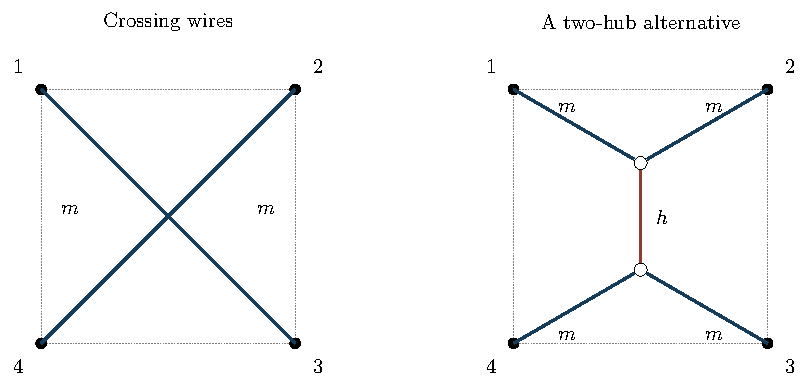
\includegraphics[width=.90\linewidth]{wire_networks.pdf}
\caption{The four black points are terminals; the two white points
are hubs. Labels on wires are their bit widths. A crossing identity
expresses the tensor on the left as a sum of alternatives of the
form on the right, possibly using the other adjacent pairing.
Choosing a summand also has a communication cost. The dotted
outline only locates the square.}
\label{fig:wires}
\end{figure}

Let $e$ be the metric on the cyclically ordered vertices $1,2,3,4$ of
a unit square: adjacent distances are $1$ and opposite distances are
$\sqrt2$. Let $e'$ also include the centre $0$, at distance $1/\sqrt2$
from each vertex.

\begin{question}\label{q:square}
Over $\C$, are $e$ and $e'$ prices in the sense of
Definition~\ref{def:price}?
\end{question}

\begin{theorem}[A non-tree price forces planar flatness]
\label{thm:intro-tree-alternative}
Fix a field $\kk$ and assume
\cite[Proposition C.3, p.~28]{Anthropic2026}.
Exactly one of the following alternatives holds:
\begin{enumerate}
\item every price on every finite party set is a tree pseudometric;
\item every finite Euclidean planar metric is a price.
\end{enumerate}
The second alternative holds if and only if some four-party price
$d$ satisfies
\[
d_{13}+d_{24}>
\max\{d_{12}+d_{34},d_{14}+d_{23}\}.
\]
Over $\C$, the first alternative makes the finite price family
equal to the family of all tree pseudometrics.
\end{theorem}

Here a tree pseudometric is a distance table obtained from points
in a real tree, allowing different labels to have distance zero.
Theorem~\ref{thm:tree-price-dichotomy} proves the statement.
The geometric ingredient is classical: a non-tree CAT(0) space
has finite planar Euclidean configurations as limits of rescaled
finite subsets, by its spaces of directions and tangent cones.
The essential source input is that Proposition C.3 realizes a
price inside a CAT(0) space whose \emph{every} finite subset is
a price. One strict four-point violation therefore suffices;
one need not prescribe the square's six distances in advance.
No such witness is constructed here over $\C$ or in
characteristic two.

\begin{theorem}[The square and planar flatness]\label{thm:introplanar}
Fix a field $\kk$ and assume the price-space embedding theorem of
\cite[Proposition C.3, p.~28]{Anthropic2026} over $\kk$.
The following are equivalent:
\begin{enumerate}
\item the unit-square metric $e$ is a price;
\item the square-with-centre metric $e'$ is a price;
\item every finite subset of the Euclidean plane is a price.
\end{enumerate}
The square can be replaced by any nondegenerate Euclidean rectangle.
\end{theorem}

Adjoining the centre therefore introduces no separate obstruction once
the geometric theorem is granted. A single planar Euclidean configuration
that is not a price excludes the square. This does not decide either
alternative and does not assert flatness in all dimensions.

The higher-dimensional statement also settles the comparison with
the OpenAI shortening condition.

\begin{theorem}[Finite flatness and strict shortening]
\label{thm:intro-flat-shortening}
Fix a field $\kk$ and an integer $D\geq2$, and assume the
price-space embedding theorem of
\cite[Proposition C.3, p.~28]{Anthropic2026}.
Let $X_D=\{\pm e_1,\ldots,\pm e_D\}\subset\mathbb R^D$,
where the $e_i$ are the standard unit vectors.
The following are equivalent:
\begin{enumerate}
\item the Euclidean metric of $X_D$ is a price;
\item the Euclidean metric of $X_D\cup\{0\}$ is a price;
\item every finite Euclidean configuration in $\mathbb R^D$ is a price;
\item no strict shortening in dimension $D$ exists over $\kk$.
\end{enumerate}
If these conditions fail, a strict shortening can be chosen
whose alternative networks use only the $2D$ terminals and
wires between nonantipodal pairs of terminals.
\end{theorem}

The proof combines Theorem~\ref{thm:cross-polytope-price-flat}
with Theorem~\ref{thm:crosspolytope-shortening}.
In particular, failure of the full flat hypothesis is equivalent
to the existence of a strict shortening in some finite dimension.
For the unit square it is enough to search for identities on
four terminals whose alternative wires run along the four sides.
This equivalence gives an exact reduction of the open question;
it does not exhibit a shortening.

The planar question also has a formulation without tensor spectra.
Let $\sigma_\C(q)$ be the least number of complex bilinear forms
$f_\nu(x,y)$ in two blocks of $q$ variables for which
\[
 \left(\sum_{i=1}^q x_i^2\right)
 \left(\sum_{j=1}^q y_j^2\right)=\sum_\nu f_\nu(x,y)^2.
\]
This is the complex form of Hurwitz's composition problem.
The crossing construction already gives
$\sigma_\C(q)\leq q^{\sqrt2+o(1)}$
\cite[Corollary 3]{Khoruzhii2026}.

\begin{theorem}[The square and the Hurwitz exponent dichotomy]
\label{thm:intro-hurwitz-dichotomy}
Assume the complex price-space theorem and spectral cover duality
of \cite[Proposition C.3 and Theorem A.6]{Anthropic2026}.
The following limit exists, with exactly the indicated alternatives:
\[
 \lim_{q\to\infty}\frac{\log\sigma_\C(q)}{\log q}
 =
 \begin{cases}
 1,&\text{if $e$ and $e'$ are not prices},\\
 \sqrt2,&\text{if $e$ and $e'$ are prices}.
 \end{cases}
\]
\end{theorem}

The proof is Corollary~\ref{cor:hurwitz-exponent-dichotomy}.
Theorem~\ref{thm:crossing-exponent-dichotomy} gives the same
alternative over every field for partial-transpose crossing rank.
A fixed improvement below the known upper exponent $\sqrt2$
would force a near-linear asymptotic construction and a strict
shortening. Conversely, any fixed superlinear lower exponent
along an unbounded sequence would force the square to be a
price and the exponent to equal $\sqrt2$. Neither bound is proved
here.

The matrix search in this criterion can be restricted by symmetry.
For clarity, the following statement defines the restricted quantity
without requiring a diagram convention.

\begin{theorem}[The structured complex crossing dichotomy]
\label{thm:intro-centralizer-dichotomy}
For $k\geq1$ put $U=(\mathbb C^2)^{\otimes k}$,
$J=\left(\begin{smallmatrix}0&1\\-1&0\end{smallmatrix}\right)^{\otimes k}$,
and $\Gamma_J=\operatorname{id}\otimes(Y\mapsto J^{-1}Y^{\mathsf T}J)$
on $\operatorname{End}(U\otimes U)$.
Let $P_{\mathrm{TL}}(k)$ be the minimum of
$\operatorname{rank}M+\operatorname{rank}N$ subject to
$I=M+\Gamma_JN$, with $M,N$ commuting with the diagonal
$\mathrm{SL}_2(\mathbb C)$ action on all $2k$ spinor factors.
Assume the complex price-space theorem and spectral cover duality
of \cite[Proposition C.3 and Theorem A.6]{Anthropic2026}.
The following limit exists and has the indicated value:
\[
 \lim_{k\to\infty}\frac{\log_2P_{\mathrm{TL}}(k)}{k}
 =\begin{cases}
 1,&\text{if the square and its centred version are not prices},\\
 \sqrt2,&\text{if both are prices}.
 \end{cases}
\]
\end{theorem}

Proposition~\ref{prop:temperley-lieb-gate} proves that the restricted
cost differs from the unrestricted partial-transpose cost by at most
$\binom{4k+3}{3}$. Its base-two logarithm divided by $k$ tends to
zero, so Theorem~\ref{thm:crossing-exponent-dichotomy} gives both
limits in the statement. The commuting operators are linear combinations
of Temperley--Lieb noncrossing pairing operators. This converts the
unrestricted problem into a structured invariant-theory problem;
the multiplicity spaces are still large, and no required rank saving
is established.

\subsection{The other principal results}

The following statements specify the algebraic and geometric
scope of the reductions. Their proofs are given in the indicated
sections; none assumes either claimed circuit separation.

\paragraph{Finite certificates.}
For a finite party set $V$, write $E=\binom V2$ and let $G_u$
be the product of binary wires with nonnegative integer load
$u\in\N^E$. A tensor is covered by other tensors when it is a
sum of their local linear restrictions.
Over any field, a nonnegative function $e$ on $E$ fails to be
a price if and only if there are loads $u,v_1,\ldots,v_r$,
integers $N,M\geq1$, and a spanning tree $T$ on $V$, such that
$G_u^N$ is covered by $M$ products of $N$ factors chosen from
the $G_{v_j}$, and
\[
 N\bigl(\langle u,e\rangle-\max_j\langle v_j,e\rangle\bigr)
   >\left(\sum_{ab\in T}e_{ab}\right)\log_2M .
\]
One can take $r\leq2|E|$.
This is Theorem~\ref{thm:finitecertificate}.
Every nonzero finite price is, moreover, exactly a positive
multiple of the wire metric of an ordinary normalized spectral
point, not merely a limit of such multiples
(Corollary~\ref{cor:price-attained}).
Strassen's spectral extension theorem applies to the semiring
of direct sums and products of wires with its inherited
restriction preorder. Verifying that preorder is the remaining
compatibility problem.

\paragraph{Named spectral families and their limitation.}
Over $\C$, the closure of scaled wire metrics of singleton
quantum functionals after arbitrary grouping is precisely the
finite union of clustered-star cones in
Theorem~\ref{thm:grouped-stars}.
The laminar extensions of Botero, Christandl, Fraser, Leigh and
Nieuwboer give precisely tree pseudometrics on wires
(Theorem~\ref{thm:laminar-tree}).
For both the square and the square with its centre, the exact
sup-norm distance to each of these families is
$(\sqrt2-1)/2$.
This is a classification of named constructions, not of all
spectral points. The generalized lower and ordered upper
quantum candidates suggested by the square's cut decomposition
fail the spectral axioms. More precisely, for any four-party cut
weights with at least two positive crossing cuts, choose two matching
wires whose internal cut is not applied first. The ordered upper
expression attains the full ambient entropy bound on their product
and strictly exceeds the product of its values on the two wires.
This exact formula holds at every wire dimension, so positive powers
and both limsup and liminf tensor-power regularizations retain the
failure of multiplicativity
(Proposition~\ref{prop:upper-matching-wires} and
Corollaries~\ref{cor:upper-power-regularization-fails}--\ref{cor:centred-upper-power-fails}).
It excludes those constructions, not a different spectral point
with the same individual-wire values.

Bug\'ar--Vrana operator geometric means offer a different construction.
Section~\ref{sec:locc-boundary} proves their exact GHZ normalization
for means supported on the three two-versus-two cuts, and gives a
sufficient criterion involving just the two diagonals of the square.
Their combined value need only exceed the tree four-point bound
as the scalar order tends to zero. With two equally weighted
crossing cuts, a fixed positive improvement over the tree
threshold suffices; the logarithmic loss from the separate
diagonal ceiling need only be strictly less than one
(Corollary~\ref{cor:binary-mean-square-sufficient}).
The equivalent lower bound must hold uniformly under GHZ factors
and tensor powers. That estimate remains open for small positive
scalar order. Exact attainment of the ceiling additionally fixes
all six distances at the prescribed normalized scale.

On the other hand every finite Euclidean metric is a
nonnegative combination of cut metrics.
Thus no homogeneous linear inequality valid on all prices
can exclude a Euclidean configuration
(Proposition~\ref{prop:no-linear-euclidean-obstruction}).

\paragraph{Shortening and characteristic.}
Over every field, a strict shortening in dimension $D$ excludes
some finite Euclidean price in that same dimension
(Theorem~\ref{thm:shortening-nonflat}).
Together with the Anthropic alternative this implies
contraction. The converse from nonflatness follows from the
price-space theorem by Theorem~\ref{thm:intro-flat-shortening}.
The implication from contraction to strict shortening remains
unresolved: the Anthropic alternative does not assert that
its two hypotheses are disjoint.
More precisely, assuming the price-space theorem, contraction
holds if and only if, for some integer $\mu\geq3$, the finite metric
\[
 \rho_\mu(A,B)=\sqrt{\operatorname{rank}(A-B)}
 \quad\text{on }\operatorname{Mat}_\mu(\mathbb F_2)
\]
is not a price over the coefficient field
(Proposition~\ref{prop:rank-price-contraction-gate}).
The binary field here labels the matrices; it need not be the
coefficient field. This metric embeds in a CAT(0) subspace complex,
so its curvature alone cannot exclude it. In any CAT(0) realization
all full-rank diameters have one common centre; a hypothetical
spectral realization therefore fixes the full edge functional on
every one of those three-party lines.
The price cone is invariant under every field extension and
therefore depends only on the characteristic
(Theorem~\ref{thm:price-characteristic}).
If a fixed finite metric is not a price over $\C$, there is a
positive integer $D_0$ such that it is not a price over any
field of characteristic $p\nmid D_0$
(Theorem~\ref{thm:nonprice-specializes}).
The integer comes from a finite certificate; its prime divisors
cannot be listed before such a certificate is found.
In particular the square question remains open here in
characteristic two as well as in characteristic zero.

\paragraph{The direct exponents.}
For the quadratic hub-displacement argument with one label
for every balanced cut and local bit budget $m\Delta\leq L$,
orthogonal edge directions with origin-to-terminal selectors
give optimal logarithmic exponent $5/4$.
The oriented-coordinate placement with the Anthropic cube
selector estimate gives optimal exponent $4/3$ under that
charged estimate. Bounded-degree expanders attain both
respective exponents; complete graphs also attain the second.
Propositions~\ref{prop:parameter-exponent}
and~\ref{prop:accounting-optimal} give the hypotheses,
parameter formula, and matching ceilings.
These are limits of the stated estimates, not of every
possible geometric circuit argument.

\paragraph{The padded permanent.}
Let the algebraically closed ground field have characteristic
different from two. Suppose, as a cited claim, that border
circuits for $\perm_m$ require more than
$B(m)=2^{a(\log_2m)^\beta}$ gates for $m\geq m_0$, where
$a>0$ and $\beta>1$.
For $N>m$ with $m^2+1\leq N^2$ and $8N^4\leq B(m)$,
the independently padded form
$z^{N-m}\perm_m$ lies outside
$\overline{\GL_{N^2}\cdot\det_N}$.
The corresponding statement for $N=m$ uses no extra variable.
This is Theorem~\ref{thm:conditional-gct}.
The claimed Anthropic and OpenAI bounds give $\beta=4/3$
and $\beta=5/4$, respectively, and imply the
Mulmuley--Sohoni conjecture for every fixed polynomial padding
exponent once $m$ exceeds the threshold written in
Corollary~\ref{cor:fixed-padding}.
Over $\C$ there is then a homogeneous highest weight equation
vanishing on the determinant cone and nonzero at some translate
of the padded permanent. The conclusion does not supply an
occurrence or multiplicity obstruction.
If the square is not a price, the claimed OpenAI stretch theorem
gives a stronger conditional conclusion: after an explicit
polynomial projection to the permanent, there are $c,\tau>0$
for which all $m\leq N\leq2^{c m^\tau/8}$ are excluded for
sufficiently large $m$.
Corollary~\ref{cor:nonflat-stretched-gct} states the constants
and onset in terms of the projection and the cited stretch theorem.

\subsection{Sources and nearby developments}

Strassen's asymptotic spectrum provides the duality and
extension framework \cite{Strassen1988,wz-spectra}.
Christandl, Vrana and Zuiddam construct the quantum functionals
\cite{cvz-universal}. Their wire values are computed here from
the definitions.
The recent equality of support and quantum functionals
\cite[Theorem I.1]{sdw-support} expands the applicable domain
of the support calculation but leaves those wire values unchanged.
The higher-party results of \cite{bcfln-quantum,alp-edge}
require a wider discussion than singleton functionals alone;
their explicitly prescribed wire metrics and their
nonconstructive extensions are distinguished below.
Bug\'ar and Vrana's operator geometric means give subadditive,
submultiplicative monotones for local operations and classical
communication (LOCC) and a spectral regularization theorem
\cite{BugarVrana2025}. Their exact flat-marginal evaluation applies
for scalar order at least one half; the boundary argument below
states the additional estimate needed to approach order zero.
The flat-rectangle argument uses the nonpositive-curvature
results of Bruhat and Tits and the standard CAT(0) literature
\cite{BT1972,BH1999,BN2008}.
The selector idea is already present in
\cite[Lemma E.7, p.~35]{Anthropic2026};
we use its sharp terminal form to obtain normalization,
finite certificates, and the shortening implication.
The geometric consequences for the permanent use the
programme of Mulmuley and Sohoni, while their
representation-theoretic scope is consistent with the
no-occurrence theorem of B\"urgisser, Ikenmeyer and Panova
\cite{MulmuleySohoni2001,BurgisserIkenmeyerPanova2019}.

The neighbouring works of Li on semidirect sums and Zhou on
weighted graph tensors provide further identity tests,
and Liu applies the Anthropic geometry to asymptotic rank
\cite{Li2026,Zhou2026,Liu2026}.
The calculations below state where these inputs constrain
normalization and where they leave an entire price ray possible.
Rossman and Zhu's partial-transpose rank
\cite[Definition 3.4]{RossmanZhu2026} gives the algebraic
form of the square obstruction.
Hrube\v{s}'s subquadratic Hurwitz construction and Khoruzhii's
subsequent $\sqrt2$ crossing bound supply its upper-bound
context \cite{Hrubes2026,Khoruzhii2026}.
Liu's two-crossing-cut argument already gives the sharp complex
Hurwitz exponent $\sqrt2$ when planar strict shortenings do not
exist \cite[Section 2, Two crossing cuts, p.~3]{Liu2026noncommutative}.
The price and tree equivalences below connect that alternative
to square-price existence and identify the complementary
exponent-one branch.

\subsection*{Reading map}
The main geometric and algebraic reductions can be read without the
later searches in particular tensor families.
\begin{center}
\begin{tabular}{p{0.34\linewidth}p{0.59\linewidth}}
Main equivalences and their inputs &
Sections~\ref{sec:foundations}--\ref{sec:planar},
\ref{sec:selectors}--\ref{sec:two-hub-cost}, and
\ref{sec:crossing-rank}--\ref{sec:field}\\[3pt]
Spectral constructions and contraction &
Sections~\ref{sec:explicit-spectrum}--\ref{sec:mixed-lines} and
\ref{sec:euclidean-contraction}\\[3pt]
Circuit and permanent consequences &
Sections~\ref{sec:graph-exponents}--\ref{sec:gct}\\[3pt]
Structured construction attempts &
Sections~\ref{sec:weight-block-gate}--\ref{sec:one-particle-digits}\\[3pt]
Concrete identities and remaining scope &
Sections~\ref{sec:identity-catalogue}--\ref{sec:open}
\end{tabular}
\end{center}

\section{Proof overview}

The sharper planar alternative comes from looking at a price
space at small scales. If a CAT(0) space is not a real tree,
two geodesics somewhere make an angle strictly between zero and
$\pi$. The completed tangent cone then contains a Euclidean
sector. Every finite planar configuration fits in that sector
after translation and is approximated by rescaled finite subsets
of the original space. The price-space theorem keeps all those
subsets inside the price family, whose closure keeps their limit.
Consequently a negative answer for the square forces every
price to be a tree pseudometric. Its four-point rule is stronger
than the CAT(0) quadrilateral inequality. Spectral cover duality
turns that rule into side-wire products with total width twice
the crossing width and only a subexponential number of terms.
Each such product has small rank across one of the two adjacent
cuts, giving crossing exponent one. The positive branch instead
forces the known exponent $\sqrt2$ to be sharp.

A finite sum identity first gives an additive term $\log_2A$, where
$A$ is the number of summands. Scaling the spectral metric also scales
this term, so it cannot simply be erased in a limit.
We retain the scale in the elementary inequality and examine when
selectors or families of identities make the comparison homogeneous.
The terminal selector also converts each relaxed spectral point
into a power of an ordinary additive one.
Compactness then replaces a limiting finite price by an exact
spectral realization. To exclude such a realization, a closed-cone
separation argument supplies finitely many integer linear forms.
Their maximum, rather than a single linear form, is needed
because Euclidean metrics already lie in the cut cone.
Strassen duality turns the separating inequality into an
asymptotic cover, and the selector turns a sufficiently large
member of that family into one finite certificate.
For the four-side normal form, every side crosses exactly one
of the two adjacent-pair cuts. Each alternative therefore has
rank at most the exponential of half its total width across
one of those cuts. Grouping by that cut yields an improved
partial-transpose exponent. Conversely, an improved exponent
routes two summands through hubs with a fixed geometric saving,
which pays for their constant selector cost for large wire dimensions.
Polarizing a bilinear sum-of-squares identity compares the two
algebraic quantities within a fixed multiplicative factor.
To impose diagonal symmetry, average each decomposition over a
compact orthogonal or spinor group. The entries of its conjugation
operator have degree linear in the number of copies but use a fixed
number of variables. Its linear span consequently has polynomial
dimension. The average is an exact linear combination of that many
rank-preserving conjugations, which bounds its rank overhead.
For spinors an explicit change in the transpose convention makes
the average compatible with the partial-transpose equation.

The exact Euclidean realizations use rigidity in nonpositive curvature.
The Euclidean diagonal lengths force the geodesics filling a rectangle
to have Euclidean distances. Filling in two directions yields an
isometric square, which contains a scaled copy of every finite planar
configuration. The field enters through the price-space theorem.
For a cross-polytope, the pairwise flat squares give orthogonal
lines in a tangent cone. Parallel-set splitting puts those lines
in a common Euclidean flat, and the Kirszbraun extension theorem
lifts the convex hull into the original space.
For the converse shortening argument, normalize all
nonantipodal distances to be at most one. The CAT(0)
quadrilateral inequality makes the Euclidean cross-polytope
the unique maximizer of the sum of antipodal distances.
If that metric is absent from the closed price cone,
compactness gives a strict gap. Cover duality converts the gap
into side-wire alternatives with a subexponential number of
selectors, which the strict geometric saving pays for.
In contrast, the characteristic result uses finite algebra:
specialize the coefficients of a certificate to a finite field
extension, descend its tensor powers, and let the fixed
extension-degree overhead be absorbed by the strict gap.

The ordered quantum obstruction is representation-theoretic.
A square Young diagram gives a one-dimensional determinant factor at
each party and a self-conjugate symmetric-group representation.
Its sign pairings have nonzero mutual overlaps, so successive crossing
projectors keep a nonzero vector even at their largest possible
entropies. Two separate wires cannot simultaneously account for that
value. In the operator-mean construction a single product tests
whether one dominated spectral point exceeds the tree bound
on the diagonal sum. The non-tree criterion then supplies a
square price. If the diagonal values attain their ceilings,
the quadrilateral inequality also fixes the individual sides.
Exact GHZ normalization follows by measuring one party when only
two-versus-two cuts occur. More generally, the growth exponent on GHZ
tensors normalizes a power-regularized upper functional.
Compactness at scalar order zero removes the norm costs of arbitrary
local linear maps.

For geometric complexity theory, dehomogenization and homogenization
of an affine matrix provide continuous maps that respect border
limits. A division-free determinant circuit translates a border
circuit bound into orbit-closure exclusion. The subsequent
representation-theoretic argument requires characteristic zero and
does not itself give an occurrence or multiplicity obstruction.

\section{Wire exponents and the scale in a sum identity}
\label{sec:foundations}

This section records the elementary algebra needed to interpret a
wire identity as an inequality of distances. We follow
\cite[Definitions A.1 and A.4, pp.~19--20]{Anthropic2026}.
A tensor on a finite nonempty set $I$ of parties belongs to
$\bigotimes_{v\in I}\kk^{n_v}$, with each $n_v\ge1$.
Products group indices by party. A restriction has the form
$s=(\bigotimes_v A_v)t$ for linear maps $A_v$.
A cover of $s$ by $t_1,\ldots,t_A$ is an equality
$s=\sum_j s_j$ with each $s_j$ a restriction of $t_j$.
The empty sum is allowed and is a cover of the zero tensor.

\begin{definition}\label{def:price}
A spectral point is a nonnegative function $\phi$ on tensors with
$\phi(1)=1$, $\phi(st)=\phi(s)\phi(t)$, and
$\phi(s)\le\sum_j\phi(t_j)$ for every cover.
For distinct parties $u,v$, the wire $\langle q\rangle_{uv}$
is a rank-$q$ identity matrix, with one-dimensional indices elsewhere.
Its exponent is defined by
$\phi(\langle q\rangle_{uv})=q^{d_\phi(u,v)}$.
A price is a pointwise limit of functions $c\,d_\phi$, with $c\ge0$.
On an infinite set, every pullback to a finite set must be a price.
\end{definition}

\begin{lemma}[Wire exponents]\label{lem:wire}
The exponents exist, belong to $[0,1]$, and, with
$d_\phi(u,u)=0$, define a pseudometric.
For every nonempty $P\subseteq I$, the diagonal tensor
$\langle q\rangle_P=\sum_{i=1}^q\bigotimes_{v\in P}e_i$
has value $q^{g_\phi(P)}$ with $g_\phi(P)\in[0,1]$.
For every tree $T$ on $P$,
$g_\phi(P)\le\sum_{\{u,v\}\in E(T)}d_\phi(u,v)$.
\end{lemma}

\begin{proof}
This is \cite[Lemma A.2, p.~19]{Anthropic2026}; we give its
normalization details. The function $f(q)=\phi(\langle q\rangle_P)$
is multiplicative and nondecreasing on positive integers, by the
product and restriction identities for diagonal tensors.
It is at least $1$, since every nonzero tensor restricts to $1$.
For integers $a,b>1$, set $r_n=\lfloor n\log a/\log b\rfloor$.
The inequalities $b^{r_n}\le a^n<b^{r_n+1}$ give
$r_n\log f(b)\le n\log f(a)\le(r_n+1)\log f(b)$.
Dividing by $n$ and taking the limit shows that
$\log f(a)/\log a$ is independent of $a$. Covering the diagonal
tensor by $q$ rank-one tensors bounds the exponent by $1$.

Contracting the middle indices of
$\langle q\rangle_{uv}\langle q\rangle_{vw}$ by the equality
functional produces $\langle q\rangle_{uw}$.
Restriction monotonicity gives the triangle inequality; symmetry
is immediate. For a tree, each vertex keeps only equal incident
indices and outputs their common value. Connectedness makes all
surviving indices equal, so the resulting tensor is
$\langle q\rangle_P$. This proves the tree bound.
A singleton diagonal tensor is equivalent to the nonzero scalar
tensor, so its exponent is $0$.
\end{proof}

We also write $U_q(P)=\langle q\rangle_P$ for the diagonal, or GHZ,
tensor, and $U_q=U_q(I)$ when the party set is understood.
When a distinction is needed, we call a point from
Definition~\ref{def:price} \emph{relaxed}. An \emph{ordinary normalized
spectral point} is such a point that is additive under local direct
sums and satisfies $\psi(U_q(I))=q$ for every positive integer $q$.
Theorem~\ref{thm:normalization} explains the relation between the two
notions.

For a wire product $T=\prod_e\langle q_e\rangle_{u_ev_e}$ put
$L_d(T)=\sum_e(\log_2q_e)d(u_e,v_e)$. Its load vector $w(T)$
has coordinate $\sum_{e:\{u_e,v_e\}=\{u,v\}}\log_2q_e$
at the unordered pair $\{u,v\}$.
Thus $\log_2\phi(T)=L_{d_\phi}(T)=\langle w(T),d_\phi\rangle$.

\begin{proposition}[Finite-cover inequality]\label{prop:cover}
If a wire product $S$ is covered by $T_1,\ldots,T_A$, with $A\ge1$,
then
\[
 2^{L_{d_\phi}(S)}\le\sum_{j=1}^A2^{L_{d_\phi}(T_j)},\qquad
 L_{d_\phi}(S)\le\max_j L_{d_\phi}(T_j)+\log_2A.
\]
If $c\,d_\phi=e$, with $c>0$, and
$\Delta=L_e(S)-\max_jL_e(T_j)>0$, then
$\Delta\le c\log_2A$.
Writing instead $d_\phi=\lambda e$ gives
$\lambda\Delta\le\log_2A$.
\end{proposition}

\begin{proof}
Use the cover axiom, multiplicativity, and the bound of a sum by
$A$ times its largest summand. Take logarithms and then scale.
\end{proof}

The multiplying scale $c$ is bounded below by $\Delta/\log_2A$,
whereas $\lambda$ in $d_\phi=\lambda e$ is bounded above by
$\log_2A/\Delta$. For $A=1$, positive saving is impossible.
For $A>1$, an additive $\log_2A$ cannot simply be discarded in a
limit defining a price.

\begin{lemma}[Homogeneous families of covers]\label{lem:homogeneous}
Suppose $S_n$ is covered by $T_{n,1},\ldots,T_{n,A_n}$ on a fixed
finite party set. Let $b_n\to\infty$, $\log_2A_n=o(b_n)$, and
$b_n^{-1}w(S_n)\to w$.
If the normalized loads of all $T_{n,j}$ approach, uniformly in
$j$, a fixed finite set $\{v_1,\ldots,v_r\}$, then every price $d$
satisfies
\[
 \langle w,d\rangle\le\max_{\beta\le r}\langle v_\beta,d\rangle.
\]
\end{lemma}

\begin{proof}
Fix a spectral point, divide the finite-cover inequality by $b_n$,
and take the limit. Uniform approximation of the loads justifies
the maximum. The resulting inequality is continuous and homogeneous,
so it passes to nonnegative multiples and pointwise limits.
The limit in $n$ precedes the limit defining the price.
\end{proof}

\begin{example}\label{ex:tensor-power-selector}
The $n$th power of an $A$-term cover has saving $n\Delta$ and at
most $A^n$ summands. The elementary inequality remains
$\lambda\Delta\le\log_2A$. Taking powers alone, without organizing
the summands or introducing another identity, does not satisfy
the subexponential hypothesis of Lemma~\ref{lem:homogeneous}.
\end{example}

\section{Non-tree curvature forces planar limits}
\label{sec:nontree-planar}

The geometric input in this section is a classical consequence of
Alexandrov angles and tangent cones.  Kleiner's dimension theorem gives
a broader account of Euclidean balls arising as rescaled subset limits
\cite[Theorem A(3), p.~2 of the author preprint]{Kleiner1999}.
We give the two-dimensional argument needed here, using the first
variation formula and the completed tangent-cone theorem of
\cite[II.3.6, II.3.18--3.19, pp.~185, 190--192]{BH1999}.
An $\mathbb R$-tree is a geodesic metric space in which every geodesic
triangle is a tripod.

\begin{lemma}\label{lem:nontree-angle}
If a $\cat$ space $X$ is not an $\mathbb R$-tree, some two nonconstant
geodesic segments with a common initial point have Alexandrov angle
strictly between $0$ and $\pi$.
\end{lemma}

\begin{proof}
Suppose instead that every such angle is $0$ or $\pi$.
Fix a unit-speed geodesic $\gamma:[0,L]\longrightarrow X$ and a point
$z$ outside its image.  The function
$f(t)=d(z,\gamma(t))$ is convex and $1$-Lipschitz.
For $0\le t<L$, the first variation formula gives
\[
 f'_+(t)=-\cos\angle_{\gamma(t)}(z,\gamma(L))\in\{-1,1\}.
\]
The right derivative of a convex function is nondecreasing.
It can therefore change from $-1$ to $1$ at most once.  Since $f$ is
Lipschitz and hence absolutely continuous, integration gives
\[
 f(t)=h+|t-a|\qquad(0\le t\le L)
\]
for some $a\in[0,L]$ and $h=f(a)\ge0$; the everywhere increasing and
everywhere decreasing cases correspond to $a=0$ and $a=L$.
Put $p=\gamma(a)$.  For every $t$ we have
\[
 d(z,\gamma(t))=d(z,p)+d(p,\gamma(t)).
\]
The uniqueness of geodesics in $X$ implies that $p$ lies on
$[z,\gamma(t)]$.  In particular the triangle with vertices
$z,\gamma(0),\gamma(L)$ is a tripod.  If $z$ lies on the original
segment, that conclusion is immediate.  Thus every geodesic triangle
is a tripod, proving the contrapositive.
\end{proof}

\begin{theorem}\label{thm:nontree-planar-limit}
Let $X$ be a $\cat$ space that is not an $\mathbb R$-tree.
For every finite tuple $z_1,\ldots,z_m\in\mathbb R^2$, there are
positive numbers $c_n$ and points $x_{1,n},\ldots,x_{m,n}\in X$ such
that
\begin{equation}\label{eq:nontree-planar-limit}
 \lim_{n\to\infty}c_n d_X(x_{i,n},x_{j,n})
   =\|z_i-z_j\|_2\qquad(1\le i,j\le m).
\end{equation}
No properness, local compactness, geodesic completeness, or finite
dimension is assumed.
\end{theorem}

\begin{proof}
By Lemma~\ref{lem:nontree-angle}, there are a point $p\in X$ and two
geodesic directions at $p$ whose angle is $\theta\in(0,\pi)$.
Let $\Sigma_pX$ be the completed space of directions.
The tangent-cone theorem says that $\Sigma_pX$ is $\mathrm{CAT}(1)$
and that its Euclidean cone is the completed $\cat$ tangent cone
$T_pX$ \cite[II.3.19, p.~191]{BH1999}.
The two directions are joined in $\Sigma_pX$ by a geodesic arc of
length $\theta$.  Distances on this arc agree with their parameter
differences.  Consequently its cone has distance formula
\[
 d\bigl((r,s),(r',s')\bigr)^2
 =r^2+(r')^2-2rr'\cos|s-s'|,
 \qquad s,s'\in[0,\theta],
\]
and is an isometrically embedded Euclidean sector of angle $\theta$.
Every finite planar set fits in this sector: a disk containing the
set can be translated sufficiently far along the sector's bisector.
We may therefore regard the given tuple as points
$v_1,\ldots,v_m\in T_pX$ with the same pairwise distances.

We next verify explicitly the finite approximation property of the
completed tangent cone.  Fix $\varepsilon>0$.  The cone of actual
geodesic germs is dense in $T_pX$, so choose germ vectors $w_i$ with
$d_{T_pX}(v_i,w_i)<\varepsilon$.
Represent each $w_i$ by a constant-speed geodesic
$\gamma_i:[0,t_0]\longrightarrow X$ starting at $p$, after shortening
their finitely many domains to one common interval.
The zero vector can be represented by the constant geodesic.
The definition of the Alexandrov angle, together with the Euclidean
comparison cosine law, gives
\[
 \lim_{t\downarrow0}\frac{d_X(\gamma_i(t),\gamma_j(t))}{t}
   =d_{T_pX}(w_i,w_j).
\]
Because there are only finitely many pairs, a single $t>0$ makes
each of these errors smaller than $\varepsilon$.
The triangle inequality in the tangent cone now gives
\[
 \left|\frac{d_X(\gamma_i(t),\gamma_j(t))}{t}
       -d_{T_pX}(v_i,v_j)\right|<3\varepsilon
 \qquad\text{for every }i,j.
\]
Apply this construction with $\varepsilon\downarrow0$, putting
$c_n=1/t_n$ and $x_{i,n}=\gamma_{i,n}(t_n)$.
This proves~\eqref{eq:nontree-planar-limit}.
The argument approximates only finitely many distance entries at a
time, so it does not require compactness of metric balls.
\end{proof}

\begin{corollary}\label{cor:closed-metric-planar-family}
Let $\mathcal M$ be a collection of finite pseudometrics closed under
restriction, positive rescaling, and pointwise limits on each fixed
finite label set.  If every finite subset of a non-tree $\cat$ space
has its metric in $\mathcal M$, then every finite Euclidean planar
metric belongs to $\mathcal M$.
\end{corollary}

\begin{proof}
Each rescaled finite distance table in
Theorem~\ref{thm:nontree-planar-limit} belongs to $\mathcal M$.
Its pointwise limit does as well.
\end{proof}

The conclusion concerns limits of rescaled finite configurations.
It does not assert that $X$ itself contains a flat square: a
hyperbolic plane, for example, is a non-tree $\cat$ space whose small
rescaled configurations approach Euclidean ones.  In the application
to prices, the remaining input is a $\cat$ realization whose entire
metric is a price on every finite subset.

\section{A non-tree price already forces the square}
\label{sec:tree-prices}

The price-space theorem has a stronger consequence than an embedding
into a space of nonpositive curvature.  The space it constructs has
a price on every finite subset.  Combining that assertion with the
preceding finite tangent-cone limits makes a strict four-point
inequality an exact test for planar flatness.

A \emph{tree pseudometric} is a pseudometric whose quotient by zero
distances embeds isometrically in an $\mathbb R$-tree.  A finite
configuration in such a tree has a finite spanning subtree.  Its
four-point distances obey the familiar rule that the two largest
of the three matching sums are equal.
The scale-free ratio of one matching sum to the larger of the
other two is the quadrilateral constant studied by Dragomir and
Nicas \cite[definition on p.~1042; Theorem 4.1 and Corollary 4.1,
p.~1053]{DragomirNicas2021}. Their CAT(0) upper bound is $\sqrt2$.
Here the price-space realization and finite-limit closure supply
the connection from a strict tree violation to a square price.

\begin{theorem}[A strict non-tree witness is sufficient]
\label{thm:tree-price-dichotomy}
Fix a field $\kk$ and assume
\cite[Proposition C.3, p.~28]{Anthropic2026}.
The following are equivalent:
\begin{enumerate}
\item the unit-square metric is a price over $\kk$;
\item some finite price over $\kk$ is not a tree pseudometric;
\item a four-party price $d$, after relabeling its parties, satisfies
\begin{equation}\label{eq:strict-tree-price-witness}
d_{13}+d_{24}>
\max\{d_{12}+d_{34},d_{14}+d_{23}\};
\end{equation}
\item an ordinary normalized spectral point $\psi$ on four parties satisfies
\begin{equation}\label{eq:strict-tree-spectral-witness}
\psi(\langle2\rangle_{13}\langle2\rangle_{24})>
\max\{\psi(\langle2\rangle_{12}\langle2\rangle_{34}),
       \psi(\langle2\rangle_{14}\langle2\rangle_{23})\}.
\end{equation}
\end{enumerate}
If these conditions fail, every price on every finite party set is a
tree pseudometric.  Over $\C$, that negative branch makes the entire
finite price family equal to the tree pseudometric family.
\end{theorem}

\begin{proof}
For a unit square the three matching sums are $2\sqrt2,2,2$.
It is therefore enough to justify the tree rule, the implication
from a non-tree price to a square price, and the spectral formulation.

For four points in a real tree, take their finite spanning subtree.
After allowing pendant edges of length zero, its shape consists of
four pendant edges and one central connecting segment; the central
segment may also have length zero.  If the pendant lengths sum to
$p$ and the central length is $b$, the three matching sums are
$p,p+2b,p+2b$ in some order.  This follows by counting how often each
edge lies on the two paths in a matching.  The two largest sums are
equal, including when points coincide.  Thus a strict inequality
as in~\eqref{eq:strict-tree-price-witness} is impossible in a tree.

Now let $d$ be a finite price that is not a tree pseudometric.
Proposition C.3 realizes it as a pullback of the metric of a
\emph{price space}.  The unnumbered definition in
\cite[Section C.4, p.~28]{Anthropic2026} requires such a space to be
complete and $\cat$, with its metric a price on every finite subset.
This last requirement is essential here.  The realizing space $X$
cannot be an $\mathbb R$-tree, since $d$ would then be a tree
pseudometric.  Corollary~\ref{cor:closed-metric-planar-family}
applies to the family of prices, which is closed under restrictions,
positive rescaling, and finite pointwise limits.  It shows that
every finite Euclidean planar metric, and in particular the unit
square, is a price.

Finally, Corollary~\ref{cor:price-attained} writes a nonzero finite
price as $d=c\,d_\psi$ for an ordinary normalized spectral point
and $c>0$.  Divide~\eqref{eq:strict-tree-price-witness} by $c$,
exponentiate to base two, and use multiplicativity on the two wires.
This gives~\eqref{eq:strict-tree-spectral-witness}.  Conversely the
wire metric of such a point is itself a price and satisfies the
strict four-point inequality.  The square supplies the witness
for the other direction.

If no square price exists, the implication just proved excludes
every non-tree finite price.  Over $\C$, the converse inclusion of
all tree pseudometrics in the price family is
Theorem~\ref{thm:laminar-tree}.  This last assertion uses that complex
spectral construction; no realization of all trees over an arbitrary
field is needed for the preceding equivalences.
\end{proof}

\begin{corollary}[The diagonal objective has only two values]
\label{cor:tree-price-objective}
Under the same price-space hypothesis, define
\[
R_\square(\kk)=
\max_{\substack{d\in\Price_\kk(\{1,2,3,4\})\\
d_{12},d_{23},d_{34},d_{41}\le1}}(d_{13}+d_{24}).
\]
Then
\[
R_\square(\kk)=
\begin{cases}
2,&\text{if the square is not a price},\\
2\sqrt2,&\text{if the square is a price}.
\end{cases}
\]
\end{corollary}

\begin{proof}
The maximum exists: the defining set is closed, and the triangle
inequality bounds both diagonals by two.  The quadrilateral
inequality~\eqref{eq:price-quad-square} and Cauchy's inequality give
$d_{13}+d_{24}\le2\sqrt2$.  The square realizes equality when it is
a price.

Otherwise Theorem~\ref{thm:tree-price-dichotomy} makes every
admissible $d$ a tree pseudometric.  Its matching sums satisfy
\[
d_{13}+d_{24}\le
\max\{d_{12}+d_{34},d_{14}+d_{23}\}\le2.
\]
The cut metric of $\{1,2\}\mid\{3,4\}$ is a flattening price over
every field.  Its four side values are $0,1,0,1$, and both diagonal
values are one.  It realizes the lower endpoint.
\end{proof}

The theorem changes the positive construction problem.  One need
not prescribe all six distances of a square: any strict violation
of the tree four-point rule by a price suffices.  The strict
inequality is stable under a small perturbation of its six entries.
Neither such a witness nor a proof that every price is a tree
pseudometric is established here.


\section{A square price is equivalent to planar flatness}
\label{sec:planar}

This section proves Theorem~\ref{thm:introplanar}, assuming
\cite[Proposition C.3, p.~28]{Anthropic2026}: every price is the
pullback of the metric of a complete $\cat$ space whose metric is
itself a price. The geometric rigidity below is classical
\cite[II.2.11]{BH1999}. We write out the polarization argument of
\cite[Lemma C.4(f), pp.~29, 65]{Anthropic2026}, based on the
quadrilateral inequality \cite{BN2008}.

\begin{lemma}[Flat rectangle]\label{lem:rectangle}
In a $\cat$ space suppose
\[
 d(x,y)=d(u,v)=a,\quad d(x,u)=d(y,v)=b,\quad
 d(x,v)^2=d(y,u)^2=a^2+b^2.
\]
If $p_s\in[x,u]$ and $q_t\in[y,v]$ occur at proportions
$s,t\in[0,1]$, then
$d(p_s,q_t)^2=a^2+b^2(s-t)^2$.
\end{lemma}

\begin{proof}
Define
\[
 B(p,p';r,r')=
 d(p,r')^2+d(p',r)^2-d(p,r)^2-d(p',r')^2.
\]
The quadrilateral inequality is
$B(p,p';r,r')\le2d(p,p')d(r,r')$.
Splitting both segments at $p_s,q_t$ expresses
$B(x,u;y,v)$ as a telescoping sum of four expressions.
Their upper bounds sum to $2b^2$, which is already
$B(x,u;y,v)$ by hypothesis. Hence each is an equality, including
\begin{equation}\label{eq:rectanglepolar}
 d(x,q_t)^2+d(y,p_s)^2-a^2-d(p_s,q_t)^2=2stb^2.
\end{equation}
For $t=s$, a second quadrilateral inequality bounds the first two
terms by $2s^2b^2+2a\,d(p_s,q_s)$. Thus
$(d(p_s,q_s)-a)^2\le0$ and $d(p_s,q_s)=a$.
Strong convexity of squared distance along a geodesic bounds each
of $d(x,q_s)^2$ and $d(y,p_s)^2$ by $a^2+s^2b^2$.
Their sum attains that bound, so both equalities hold.
Renaming $s$ as $t$ in the first and substituting into
\eqref{eq:rectanglepolar} gives the claim.
\end{proof}

\begin{proof}[Proof of Theorem~\ref{thm:introplanar}]
The third assertion implies the second, which implies the first
by restriction. Embed a square price in a price space and name
its vertices $x,y,v,u$ in cyclic order.
Let $l_t,r_t$ be proportion-$t$ points on its left and right
vertical edges. The lemma gives
\[
 d(l_t,r_{t'})^2=1+(t-t')^2,\qquad
 d(l_t,l_{t'})=d(r_t,r_{t'})=|t-t'|.
\]
Let $F(s,t)$ be the proportion-$s$ point on $[l_t,r_t]$.
For $t\ne t'$, the four endpoints
$l_t,r_t,r_{t'},l_{t'}$ form a rectangle with sides $1$ and
$|t-t'|$. Apply the lemma along its horizontal edges:
\[
 d(F(s,t),F(s',t'))^2=(s-s')^2+(t-t')^2.
\]
When $t=t'$, the same formula is the constant-speed geodesic
formula. Therefore the whole unit square embeds isometrically.
Every finite planar set can be translated and scaled into it.
Pullback and rescaling preserve prices, proving the third assertion.
The same construction fills any rectangle with positive area,
and every finite planar set fits in a homothetic copy of it.
\end{proof}

\begin{corollary}\label{cor:planarobstruction}
Assuming the price-space embedding theorem, the existence of any
finite planar Euclidean configuration that is not a price is
equivalent to the square not being a price.
If \cite[Theorem D.2, pp.~30--31]{Anthropic2026} also holds,
either failure implies the contracting hypothesis.
\end{corollary}

\begin{proof}
The equivalence is the contrapositive of
Theorem~\ref{thm:introplanar}. A failed planar instance refutes
the full flat hypothesis, so Theorem D.2 gives the contracting one.
\end{proof}

\subsection{Cross-polytopes detect flatness in every fixed dimension}

The four vertices of a square are the two-dimensional instance of a
more general rigid configuration. Write
\[
 X_D=\{e_1,-e_1,\ldots,e_D,-e_D\}\subset\mathbb R^D,
 \qquad C_D=\operatorname{conv}(X_D)
           =\{x:\textstyle\sum_i|x_i|\le1\}.
\]
The next statement is classical metric geometry in the sense that its
inputs are the flat-square theorem, the parallel-set splitting theorem,
the tangent-cone theorem and the Kirszbraun--Lang--Schroeder extension
theorem. We give the argument because a collection of pairwise flat
coordinate squares does not, without an additional argument, justify
the existence of a higher-dimensional flat.

\begin{lemma}[Cross-polytope rigidity]\label{lem:cross-polytope-flat}
Let $D\ge1$ and let $f:X_D\longrightarrow X$ be an isometric embedding
into a complete $\cat$ space. There is an isometric embedding
$F:C_D\longrightarrow X$ extending $f$. Its image is precisely the
closed convex hull of $f(X_D)$. In particular that hull contains an
isometric Euclidean $D$-ball of radius $1/\sqrt D$.
\end{lemma}

\begin{proof}
For $D=1$ use the geodesic between the two vertices. Suppose $D\ge2$.
Every two antipodal pairs have the metric of a Euclidean square, so
Lemma~\ref{lem:rectangle} and its filling argument give an isometric
filled square. The two diagonals in each such square have the same
midpoint. Consequently all $D$ antipodal segments have one common
midpoint, denoted by $o$.

Let $T$ be the completed tangent cone of $X$ at $o$. It is a complete
$\cat$ space by \cite[II.3.19, p.~191]{BH1999}. The logarithm map
$\log_o:X\longrightarrow T$, sending a point to its distance and
initial direction from $o$, is $1$-Lipschitz: comparison angles at $o$
are at least the Alexandrov angle, which gives
\[
 d_T(\log_o x,\log_o y)^2
 \le d_X(x,y)^2.
\]
On each filled square through $o$ it preserves Euclidean distances.
The cone over the directions of that square therefore contains a full
Euclidean plane. It follows that $T$ contains $D$ geodesic lines
$L_1,\ldots,L_D$ through its vertex, with each pair forming the
coordinate axes of an isometrically embedded Euclidean plane.

We now justify that these lines lie in one Euclidean $D$-flat. More
generally, this is true in any complete $\cat$ space with the stated
configuration of complete lines. Induct on $D$. The parallel set of
$L_1$ is convex and splits as $Y\times\mathbb R$, where the second
coordinate is projection onto $L_1$;
see \cite[II.2.14, p.~183]{BH1999}. If necessary pass to its closure,
which is the product of the completion of $Y$ with $\mathbb R$; this
closure remains a convex subspace of the given complete space. The
plane formed by $L_1$ and $L_j$ shows that $L_j$ is contained in this
parallel set and has second coordinate zero. For $j,k>1$, the entire
plane formed by $L_j$ and $L_k$ is the convex hull of those two entire
lines: a point with coordinates $(a,b)$ is the midpoint of $(2a,0)$
and $(0,2b)$. Hence this plane is in the parallel set. Its
$\mathbb R$ coordinate is zero because that coordinate is affine on
geodesics. The completed factor $Y$ thus contains $D-1$ lines with
the same pairwise-plane property. Induction gives a Euclidean
$(D-1)$-flat in that factor, and its product with $\mathbb R$ gives
the required $D$-flat. No local compactness or geodesic completeness
of $X$ has been assumed.

Identify this flat with $\mathbb R^D$ so that
$\log_o f(\pm e_i)=\pm e_i$. In particular $C_D$ is a closed convex
subset of $T$. The Kirszbraun--Lang--Schroeder theorem
\cite{LangSchroeder1997}, in the form
\cite[Theorem~10.14, p.~160]{AKP2023}, extends the vertex map $f$ to a
$1$-Lipschitz map $F:\mathbb R^D\longrightarrow X$. Here the source
is complete with curvature bounded below by zero and the target is
complete with curvature bounded above by zero, so the extension
theorem has no radius restriction. Restrict $F$ to $C_D$ and let
$P:T\longrightarrow C_D$ be nearest-point projection. Projection
onto a complete convex subset of a $\cat$ space is $1$-Lipschitz
\cite[II.2.4]{BH1999}. Thus
\[
 G=P\circ\log_o\circ F:C_D\longrightarrow C_D
\]
is $1$-Lipschitz and fixes every vertex.

The fixed set of a $1$-Lipschitz self-map of a uniquely geodesic space
is convex. Indeed, if $a,b$ are fixed and $p\in[a,b]$, the inequalities
$d(a,Gp)\le d(a,p)$ and $d(Gp,b)\le d(p,b)$ have total upper bound
$d(a,b)$, so both are equalities and uniqueness of the geodesic gives
$Gp=p$. Therefore $G$ fixes the convex hull of its vertices, namely
all of $C_D$. For $p,q\in C_D$ we consequently have
\[
 \|p-q\|=d_T(Gp,Gq)
 \le d_T(\log_o Fp,\log_o Fq)
 \le d_X(Fp,Fq)\le\|p-q\|.
\]
Every inequality is an equality, proving that $F|_{C_D}$ is isometric.
Its image is convex by uniqueness of geodesics, is closed by
compactness, and is generated by the images of the vertices under
finite convex combinations. It is therefore their closed convex
hull. Finally $\sum_i|x_i|\le\sqrt D\|x\|$ shows that $C_D$ contains
the claimed ball.
\end{proof}

A recent, stronger variance-rigidity statement also implies this
lemma: \cite[Proposition~1.4 and Section~13.1]{Lytchak2026geometry}
states that equality in the $\cat$ variance inequality forces the
closed convex hull of the measure's support to be a convex subset of
a Hilbert space. For the uniform measure on $f(X_D)$, the midpoint
inequality for each antipodal pair gives
\[
 \frac1{2D}\sum_{v\in X_D}d(z,f(v))^2\ge1+d(z,o)^2,
 \qquad
 \frac1{(2D)^2}\sum_{u,v\in X_D}d(f(u),f(v))^2=2.
\]
Thus $o$ is its barycentre with variance $1$, and equality holds in
that criterion. The preceding proof uses the classical extension and
splitting theorems directly and does not require the newer preprint.

\begin{theorem}[A finite test for flatness in dimension $D$]
\label{thm:cross-polytope-price-flat}
Fix a field and $D\ge1$. Assume
\cite[Proposition~C.3, p.~28]{Anthropic2026}, including that every
finite subset of its complete $\cat$ price space is a price. The
following conditions are equivalent:
\begin{enumerate}
\item the Euclidean metric of $X_D$ is a price;
\item the Euclidean metric of $X_D\cup\{0\}$ is a price;
\item every finite subset of $\mathbb R^D$ has its Euclidean metric
as a price.
\end{enumerate}
\end{theorem}

\begin{proof}
The third condition implies the second and the second implies the
first by restriction. Under the first condition, embed $X_D$ into a
complete $\cat$ price space using Proposition~C.3. The embedding is
injective because the vertex distances are positive. By
Lemma~\ref{lem:cross-polytope-flat}, this space contains a Euclidean
$D$-ball of positive radius. Any finite subset of $\mathbb R^D$ can
be translated and scaled into that ball. Its image has a price
metric, and pullback followed by inverse rescaling preserves prices.
This proves the third condition.
\end{proof}

In dimension two, $X_2$ is a rotated square of side $\sqrt2$;
Theorem~\ref{thm:cross-polytope-price-flat} therefore recovers
Theorem~\ref{thm:introplanar}. In higher dimensions it supplies the
geometric step needed to compare a shortening of the $D$ coordinate
diameters with failure of flatness in that same dimension.

\IfFileExists{explicit_spectrum.tex}{\section{The explicit spectral families on wire networks}
\label{sec:explicit-spectrum}
This section computes the wire metrics of the standard explicit spectral points, including the points obtained by grouping parties, and of the more recent laminar extensions.  The distinction between these families and the whole asymptotic spectrum is essential.

Let $V$ be a finite set with at least two elements.  A split of $V$ is an unordered bipartition $S\mid V\setminus S$ into nonempty parts.  Its cut pseudometric is
\[
 \delta_S(u,v)=\begin{cases}1&\text{if exactly one of $u,v$ belongs to $S$,}\\0&\text{otherwise.}\end{cases}
\]
For a loopless multigraph $G$ on $V$, with an integer $q_e\geq1$ assigned to each edge, write
\[
 W_G=\mathop{\bigotimes}_{e=uv\in E(G)}\langle q_e\rangle_{uv},
 \qquad
 r_S(G)=\prod_{\substack{e=uv\in E(G)\\\delta_S(u,v)=1}}q_e.
\]
The tensor products here are taken party by party.  Parallel edges may be combined by multiplying their dimensions. We write $F_\theta=2^{E_\theta}$ for the lower quantum functional and its logarithm; the entropy definition is recalled in the proof below.

\begin{proposition}[Flattenings and entropy on wire products]
\label{prop:wire-evaluations}
Over any field, the matrix flattening of $W_G$ across a split $S\mid V\setminus S$ has rank $r_S(G)$.  Over $\mathbb C$, if $\theta$ is a probability distribution on the splits, the lower quantum functional satisfies
\begin{equation}
 E_\theta(W_G)=\sum_S\theta_S\log_2 r_S(G),
 \qquad
 F_\theta(W_G)=\prod_{e=uv}q_e^{\sum_S\theta_S\delta_S(u,v)}.
 \label{eq:wire-cut-entropy}
\end{equation}
In particular, for singleton weights $\theta_v\geq0$ with $\sum_v\theta_v=1$,
\begin{equation}
 F_\theta(W_G)=\prod_{e=uv}q_e^{\theta_u+\theta_v}.
 \label{eq:wire-star}
\end{equation}
Equation~\eqref{eq:wire-cut-entropy} evaluates a functional.  It does not assert that the functional for an arbitrary split distribution is a spectral point.
\end{proposition}

\begin{proof}
Choose the usual bases on the wire spaces.  A wire crossing the split contributes an identity matrix of rank $q_e$ to the flattening.  A wire wholly on either side contributes a nonzero vector on that side and hence a factor of rank one.  Matrix rank is multiplicative under a Kronecker product, proving the first assertion over every field.

For the entropy assertion, normalize each wire to
$q_e^{-1/2}\sum_{a=1}^{q_e}e_a\otimes e_a$.  The normalized tensor $W_G$ is their tensor product.  Its marginal on $S$ is a tensor product of pure states from internal wires and maximally mixed states from the crossing wires.  Its nonzero spectrum is therefore uniform on $r_S(G)$ entries, with entropy $\log_2 r_S(G)$.

The lower quantum functional is, by Christandl--Vrana--Zuiddam's Definition~3.16 in Section~3.2 of the arXiv version~\cite{cvz-universal}, the supremum of the weighted marginal entropies after invertible maps at the individual parties.  Such maps preserve every flattening rank.  A density matrix of rank $r$ has entropy at most $\log_2 r$: if its positive eigenvalues are $p_1,\ldots,p_r$, this follows from
$\sum_i p_i\log_2(p_i/(1/r))\geq0$.
Consequently every summand in the defining entropy expression is at most $\log_2 r_S(G)$.  The normalized wire tensor simultaneously attains every one of these bounds.  This proves~\eqref{eq:wire-cut-entropy}.  Each edge $uv$ crosses precisely the singleton splits at $u$ and $v$, giving~\eqref{eq:wire-star}.  For two parties the two singleton weights refer to the same split; their sum is one, so the formula still applies.
\end{proof}

The singleton functional is a universal spectral point by Christandl--Vrana--Zuiddam, Theorem~3.30 and Corollary~3.31; its moment-polytope expression is their equation~(25), p.~27 of the arXiv version.  The proposition identifies a simultaneous maximizing spectrum, so no uncomputed moment polytope is needed for these evaluations.  The distinction in its last sentence is substantive: Botero--Christandl--Fraser--Leigh--Nieuwboer prove in Theorem~3.14 of~\cite{bcfln-quantum} that, for at least four parties, every nonsingleton-supported lower quantum functional fails to be a universal spectral point.  Grouping parties before applying a singleton functional is a different operation.

\begin{proposition}[Support functionals on wire products]
\label{prop:wire-support}
For every field and every probability vector $\theta$ on $V$, both Strassen support functionals satisfy
\[
 \zeta^\theta(W_G)=\zeta_\theta(W_G)
     =\prod_{e=uv}q_e^{\theta_u+\theta_v}.
\]
\end{proposition}
\begin{proof}
We use the upper and lower support definitions in Sections~2.1--2.2 of~\cite{cvz-universal}: the logarithmic upper functional minimizes, over bases, the maximum of the weighted marginal Shannon entropies on the support; the lower one maximizes the same entropy quantity on the maximal elements of the support.  We also use their Theorem~2.15, namely $\rho_\theta\leq\rho^\theta$.

Give each edge an orientation and give distinct edges distinct nonnegative integers $j(e)$.  Choose an integer $B$ larger than twice the greatest edge dimension.  At a vertex $v$, for the local tuple $(a_e)_{e\ni v}$ with $0\leq a_e<q_e$, put
\[
 \alpha_v((a_e))=\sum_{e\ni v}\sigma(v,e)B^{j(e)}a_e,
\]
where $\sigma(v,e)$ is $1$ at one endpoint of $e$ and $-1$ at the other.  This is injective: in a nonzero difference of two local tuples, its term of largest exponent has absolute value at least $B^j$, whereas the sum of all smaller terms has absolute value less than $B^j$ by the choice of $B$.
Order the local basis by increasing $\alpha_v$.  On every support tuple of $W_G$, the sum of these labels over the vertices is zero.  Two different support tuples consequently cannot be comparable in the product order.  Thus the support is an antichain and every support element is maximal.

Choose all edge labels independently and uniformly.  At vertex $v$ the marginal is uniform on $\prod_{e\ni v}q_e$ local labels.  The lower functional is therefore at least
$\sum_v\theta_v\sum_{e\ni v}\log_2 q_e$ in logarithmic form.  The upper functional is at most the same number, since no local marginal entropy exceeds the logarithm of the local dimension, and the standard support is one of its permitted choices of basis.  The inequality $\rho_\theta\leq\rho^\theta$ makes both bounds equalities.  Exponentiating proves the claim.
\end{proof}

For complex tensors the upper support functional is now known to equal the singleton quantum functional on all tensors, by Sakabe--Do\u gan--Walter, Theorem~I.1 of~\cite{sdw-support}.  Over arbitrary fields, Alman--Li--Pratt prove universality of the three-party edge support functionals in Theorem~1.1 of~\cite{alp-edge}.  These developments extend the scope of the global spectral points; their values on wire products remain the values in Proposition~\ref{prop:wire-support}.

\subsection{Grouping parties and the closed family of clustered stars}
The next result includes all singleton quantum points obtained after grouping several of the original parties.

Let $\pi$ be a partition of $V$ into at least two nonempty blocks.  Regard a $V$-tensor as a tensor whose parties are the blocks, and apply a singleton quantum functional with probability weights $\theta_B$ on those blocks.  Grouping respects products, direct sums up to zero ambient coordinates, and restrictions.  This composition is therefore a universal spectral point.  Denote the collection of these points, for all $\pi$, by $\mathcal Q_V$.

\begin{theorem}[The scaled metrics of grouped singleton functionals]
\label{thm:grouped-stars}
The scaled wire metrics of $\mathcal Q_V$ form exactly the following set:
choose a partition $\pi$ of $V$ into at least two blocks and nonnegative numbers $a_B$, and set
\begin{equation}
 d(u,v)=\begin{cases}
 0,&B(u)=B(v),\\
 a_{B(u)}+a_{B(v)},&B(u)\ne B(v).
 \end{cases}
 \label{eq:clustered-star}
\end{equation}
This is a closed finite union of polyhedral cones.  For three labels it is the whole pseudometric cone.
\end{theorem}
\begin{proof}
A wire whose endpoints are in the same block becomes a nonzero simple tensor in the grouped system and has value one.  A wire joining different blocks becomes a bipartite wire between those blocks.  Proposition~\ref{prop:wire-evaluations} gives exponent $\theta_{B(u)}+\theta_{B(v)}$.  Scaling by $c\geq0$ gives~\eqref{eq:clustered-star} with $a_B=c\theta_B$.
Conversely, when $c=\sum_Ba_B>0$, choose $\theta_B=a_B/c$.  When all $a_B$ vanish the zero scale realizes the zero metric.

For a fixed partition the cone is the nonnegative span of its finitely many block-cut metrics $\delta_B$ and is therefore polyhedral and closed.  There are only finitely many partitions of $V$.  Finally, for three labels $1,2,3$, every pseudometric is a star with
\[
 a_1=\frac{d_{12}+d_{13}-d_{23}}2,\quad
 a_2=\frac{d_{12}+d_{23}-d_{13}}2,\quad
 a_3=\frac{d_{13}+d_{23}-d_{12}}2.
\]
The triangle inequalities make these numbers nonnegative, and substitution gives the prescribed distances.
\end{proof}

\subsection{Laminar extensions and tree metrics}
The 2026 laminar extension theorem supplies more global spectral points, although it gives their extension by existence rather than by an explicit formula on every tensor.  Its wire values admit a complete geometric description.

Two splits are \emph{compatible} if at least one of their four pairwise intersections is empty.  A split distribution is \emph{laminar} if all splits with positive weight are pairwise compatible.  Botero--Christandl--Fraser--Leigh--Nieuwboer's Proposition~4.3~\cite{bcfln-quantum}, using Strassen's extension theorem, extends the common upper and lower laminar quantum functional from their semiring of laminar-quantum-robust tensors to a universal spectral point.  Wire products belong to this semiring, by their Proposition~4.12 and closure under products.  Let $\mathcal L_V$ be the collection of all these extensions.

\begin{theorem}[The wire metrics of laminar extensions]
\label{thm:laminar-tree}
The scaled wire metrics of $\mathcal L_V$ are exactly the pseudometrics obtained by mapping $V$ into a finite tree with nonnegative edge lengths.  Their set is closed.  For three labels it is one cone with three pendant-edge generators; for four labels it is the union of the three binary-tree cones, each with five edge generators; for five labels it is the union of the fifteen binary-tree cones, each with seven edge generators.  Zero edge lengths include all degeneracies.
\end{theorem}
\begin{proof}
By Proposition~\ref{prop:wire-evaluations}, an extension associated with $\theta$ has wire metric $\sum_S\theta_S\delta_S$.  Scaling removes the normalization $\sum_S\theta_S=1$.  We show directly that the nonnegative sums of compatible cut metrics are precisely the tree pseudometrics.

Deleting any edge of a tree separates its labels into two parts, and the distance between two labels is the sum of the lengths of the edges separating them.  The resulting edge splits are pairwise compatible.  Edges with no label on one side may be removed, and labels at internal vertices may be given pendant edges of length zero.

Conversely, choose a distinguished label $r\in V$.  Represent each compatible split by the side not containing $r$.  These subsets form a laminar collection: any two are disjoint, or one contains the other.  Add $V$ and all singletons, assigning zero length to subsets not already present.  Make a vertex for each of these subsets.  Join each proper subset to the smallest strictly larger subset in the collection that contains it.  The parent is unique, since two candidate parents intersect and are therefore nested.  The resulting connected graph is a tree: every vertex except $V$ has one parent, and inclusion strictly increases along every parent edge.  Give the edge from $S$ to its parent the coefficient of $\delta_S$, or zero when $S$ was added.  Put label $v$ at vertex $\{v\}$.  The edge from $S$ to its parent separates precisely the labels in $S$ from the others, so its distance function is the required cut sum.

There are finitely many possible compatible split families on a fixed finite label set, and each determines a finitely generated closed cone.  Their union is closed.  Any nonbinary tree may be resolved into a binary tree by adding edges of length zero.  There is one binary unrooted shape with three labelled leaves, three with four, and fifteen with five: a four-leaf binary tree is determined by its $2\mid2$ split; a five-leaf binary tree is determined by choosing the middle leaf in five ways and partitioning the other four labels into its two unordered cherries in three ways.  A binary tree with $n$ leaves has $2n-3$ edges, by the degree sum and Euler's formula.  This gives the stated counts of generators.
\end{proof}

\begin{theorem}[Exact distance from the square]
\label{thm:square-tree-gap}
Let $e$ be the metric of a unit square, labelled cyclically $1,2,3,4$, and let $e'$ include its centre $0$.  In the supremum norm on unordered pairs,
\[
 \operatorname{dist}(e,\{c\,d_F:F\in\mathcal Q_V,\ c\geq0\})
 =\operatorname{dist}(e,\{c\,d_F:F\in\mathcal L_V,\ c\geq0\})
 =\frac{\sqrt2-1}{2}.
\]
The same two equalities hold for $e'$ on its five labels.
\end{theorem}
\begin{proof}
For any four points in a tree, the two largest of
\[
 d_{12}+d_{34},\qquad d_{13}+d_{24},\qquad d_{14}+d_{23}
\]
are equal.  Indeed, after pruning and suppressing unlabelled degree-two vertices, the minimal subtree connecting the points has either one central vertex, in which case all three sums agree, or a central path separating two pairs.  Each sum contains every pendant segment once.  The pairing within the two sides omits the central path, and each of the other pairings contains it twice.  Zero lengths and coincident labels follow by the same formula.

For the square the three sums are $2,2\sqrt2,2$.  If a tree pseudometric $d$ is within $\varepsilon$ of $e$, its middle-labelled sum is at least $2\sqrt2-2\varepsilon$, while the other two sums are at most $2+2\varepsilon$.  If $\varepsilon<(\sqrt2-1)/2$, the middle-labelled sum would be strictly larger than both others, contradicting the tree property.  Restricting a tree metric on the square and centre to the four corners gives the same lower bound for $e'$.

For the matching upper bound, put four labelled leaves on a star, each with pendant length
\[
 a=\frac{1+\sqrt2}{4}.
\]
Every distance between corners is $2a=(1+\sqrt2)/2$, whose deviations from $1$ and $\sqrt2$ are both $(\sqrt2-1)/2$.  For $e'$, add a fifth leaf labelled $0$, of pendant length
\[
 a_0=\frac{\sqrt2-1}{4}.
\]
Then its distance to each corner is $a_0+a=\sqrt2/2$, exactly the required radial distance.  These stars belong to $\mathcal Q_V$ after scale by Theorem~\ref{thm:grouped-stars}; they also belong to $\mathcal L_V$.  Finally every clustered star is itself a tree pseudometric, so the lower bound applies to both families.
\end{proof}

Theorem~\ref{thm:square-tree-gap} excludes these spectral constructions, including their pointwise limits.  It does not exclude the square from the price cone.  In particular it is not a classification of all spectral points, and the existence of other higher-party spectral points is already proved in~\cite{alp-edge,bcfln-quantum}.

\begin{corollary}[Cross-polytope configurations]
\label{cor:cross-polytope-tree-gap}
For $D\geq2$, give $X_D=\{\pm e_1,\ldots,\pm e_D\}$ its Euclidean metric, with or without the centre $0$.  Its exact distance in the sup norm to both the scaled grouped-singleton family and the scaled laminar-tree family is
\[
 1-\frac1{\sqrt2}.
\]
For $D=1$ the distance is zero.
\end{corollary}
\begin{proof}
Two antipodal pairs form a square with side $\sqrt2$ and diagonals two.  The four-point argument in Theorem~\ref{thm:square-tree-gap} therefore gives the lower bound $\sqrt2(\sqrt2-1)/2=1-1/\sqrt2$.  For the upper bound take a star whose terminal pendant edges all have length $(2+\sqrt2)/4$.  Every terminal distance is $(2+\sqrt2)/2$, at exactly the asserted error from either possible Euclidean distance, $\sqrt2$ or two.  If the centre is included, give it a pendant edge of length $(2-\sqrt2)/4$; all its terminal distances are then exactly one.  These are singleton star metrics.  The configurations for $D=1$ lie on a line and are already tree metrics.
\end{proof}

\begin{corollary}[Extra parties do not remove this gap]
\label{cor:tree-pullbacks}
Starting with any of the tree metrics of Theorem~\ref{thm:laminar-tree}, adding finitely many parties, pulling back along maps of label sets, and taking pointwise limits cannot produce the square or the square with its centre.
\end{corollary}
\begin{proof}
A pullback is obtained by composing the map into the same weighted tree with a map of label sets.  It is again a tree pseudometric.  The tree-pseudometric cone on the final finite label set is closed, and Theorem~\ref{thm:square-tree-gap} gives a positive distance from it.
\end{proof}

\subsection{An exact formal candidate and its missing extension}
The following calculation records why excluding trees alone leaves the main problem open.
Put $a=1-\sqrt2/2$ and $b=\sqrt2-1$.  On the four corners,
\begin{equation}
 e=a\sum_{i=1}^{4}\delta_{\{i\}}
       +b\bigl(\delta_{\{1,2\}}+\delta_{\{1,4\}}\bigr).
 \label{eq:square-cut-decomposition}
\end{equation}
A side crosses one of the two displayed $2\mid2$ cuts and two singleton cuts, so its value is $2a+b=1$.  A diagonal crosses both of those cuts and two singleton cuts, so its value is $2a+2b=\sqrt2$.  The total cut weight is $4a+2b=2$.  The two nonsingleton splits are incompatible.
For the square and centre, set $t=(\sqrt2-1)/2$.  Then
\begin{equation}
 e'=a\sum_{i=1}^{4}\delta_{\{i\}}
       +t\bigl(\delta_{\{1,2\}}+\delta_{\{2,3\}}
                 +\delta_{\{3,4\}}+\delta_{\{4,1\}}\bigr).
 \label{eq:centred-square-cut-decomposition}
\end{equation}
Here a side has value $2a+2t=1$, a diagonal has value $2a+4t=\sqrt2$, and a radial pair has value $a+2t=\sqrt2/2$.  Again the weights sum to two.

Thus the lower quantum functionals for half of the weights in~\eqref{eq:square-cut-decomposition} and~\eqref{eq:centred-square-cut-decomposition} have exactly the wire metrics $e/2$ and $e'/2$.  Theorem~3.14 of~\cite{bcfln-quantum} rules out using these lower functionals themselves as universal spectral points.  A universal spectral point agreeing with them on wire products, if one exists, must be obtained by a further extension argument.  The laminar extension theorem does not supply that argument, because the required cuts cross.  This is a precise obstruction to the proposed entropy construction, not a proof of nonexistence of the desired spectral point.

\subsection{Why singleton-anchor interpolation cannot create a flat square}
The obstruction also applies to interpolation from an arbitrary price, not merely from the families classified above.  This uses the quadrilateral inequality for prices proved through the CAT$(0)$ embedding theorem.

\begin{proposition}[The square has no positive pendant summand]
\label{prop:square-no-pendant}
Assume that every price $d$ satisfies
\begin{equation}
 d_{13}^2+d_{24}^2
 \leq d_{12}^2+d_{23}^2+d_{34}^2+d_{41}^2.
 \label{eq:price-quadrilateral}
\end{equation}
If $a_1,\ldots,a_4\geq0$ and the off-diagonal function
$d_{ij}=e_{ij}-a_i-a_j$ is a price, then every $a_i$ is zero.  For the square with centre, the same conclusion holds for $a_0,\ldots,a_4\geq0$ and $d_{ij}=e'_{ij}-a_i-a_j$.
\end{proposition}
\begin{proof}
Put $t=1-\sqrt2/2>0$ and $s=a_1+a_2+a_3+a_4$.  The triangle inequality for the triple consisting of $i$ and its two cyclic neighbours gives
\[
 0\leq d_{i-1,i}+d_{i,i+1}-d_{i-1,i+1}
       =2-\sqrt2-2a_i.
\]
Thus $0\leq a_i\leq t$ for every corner.  Let $D(d)$ be the left side of~\eqref{eq:price-quadrilateral} minus its right side.  Direct expansion gives
\[
 D(d)=4ts-\sum_i a_i^2
       +2(a_1a_3+a_2a_4)
       -2(a_1a_2+a_2a_3+a_3a_4+a_4a_1).
\]
Since $a_i^2\leq ta_i$ and $2a_ia_j\leq t(a_i+a_j)$, the two negative sums have total absolute value at most $ts+2ts=3ts$.  The opposite-pair contribution is nonnegative.  Hence $D(d)\geq ts$.  The assumed quadrilateral inequality forces $s=0$ and therefore every corner coefficient vanishes.

For five labels, restriction to the corners gives the same conclusion.  In fact, regardless of the corner coefficients, the triangle inequality along either diameter through the centre gives
\[
 0\leq d_{10}+d_{03}-d_{13}=-2a_0,
\]
so $a_0=0$ as well.
\end{proof}

Wigderson--Zuiddam's graph-spectrum interpolation theorem is log-star-convexity toward a single-party flattening; see Section~12.7, Theorem~12.23 in the author version of~\cite{wz-spectra}.  In wire exponents this is interpolation $d\mapsto(1-\lambda)d+\lambda\delta_{\{v\}}$.  Proposition~\ref{prop:square-no-pendant} shows that no finite succession of such interpolations with a positive final pendant contribution can give either square configuration, even if the starting price is arbitrary.  Local changes of tensor bases give no additional freedom: restriction monotonicity in both directions makes every spectral point invariant under invertible maps at the parties.  The symmetric-space and moment-polytope descriptions may still lead to other constructions, but neither coordinate changes nor these known anchor interpolations supply one.

\subsection{Every crossing four-party upper quantum expression fails}
The formal cut decomposition does not become a spectral point by replacing the lower quantum functional with the ordered upper quantum functional.  In fact every four-party weighting with crossing split support fails already on the rank-two unit tensor.  This strengthens the crossing-projector example in Appendix~D of Botero--Christandl--Fraser--Leigh--Nieuwboer~\cite{bcfln-quantum} by allowing arbitrary singleton weights and all three nonsingleton splits.

For clarity, the ordered upper expression uses a different definition.
For a partition $\lambda\vdash n$, let $H(\lambda/n)$ be the base-two
Shannon entropy of its normalized row lengths, and let
$P^{(b)}_\lambda$ be the Schur--Weyl isotypic projector for the grouped
cut $b$, on the globally symmetric subspace of the $n$ tensor copies.
For a nonzero tensor $T$ and an ordering $b_1,\ldots,b_s$ of the
positive-weight cuts, the definition in
\cite[Definition 3.3]{cvz-universal} is
\[
 E^\theta(T)=\sup\left\{
   \sum_{j=1}^s\theta(b_j)H(\lambda_j/n):
   n\geq1,\ \lambda_j\vdash n,\quad
   P^{(b_s)}_{\lambda_s}\cdots P^{(b_1)}_{\lambda_1}
   T^{\otimes n}\ne0\right\}.
\]
We put $F^\theta(T)=2^{E^\theta(T)}$ and $F^\theta(0)=0$.
The order is part of the expression when the cut projectors do not
commute. Thus any one nonzero ordered projector tuple proves the
corresponding entropy lower bound.

\begin{proposition}[Failure of crossing upper quantum functionals]
\label{prop:square-upper-fails}
Let $\theta$ be a probability distribution on the bipartitions of four parties, with at least two positive weights on the three $2\mid2$ splits.  List those positive-weight splits in the order in which their projectors are applied, as $b_1,\ldots,b_r$, where $r\in\{2,3\}$.  For the ordered upper quantum functional and the unnormalised unit tensor $U_2=\sum_{i=0}^{1}e_i^{\otimes4}$,
\begin{equation}
 E^\theta(U_2)\geq 1+\sum_{j=2}^r\theta(b_j)>1.
 \label{eq:upper-square-failure}
\end{equation}
Thus $F^\theta$ fails even the cover inequality for relaxed spectral points.  For the square weights in~\eqref{eq:square-cut-decomposition}, divided by two, either order gives
\[
 E^\theta(U_2)\geq\frac{1+\sqrt2}{2}>1.
\]
\end{proposition}
\begin{proof}
We use four tensor copies.  Assign Young shape $(2,2)$ to every singleton split and to $b_1$, and shape $(1,1,1,1)$ to every subsequent $2\mid2$ split.  We prove that the corresponding ordered projector product on $U_2^{\otimes4}$ is nonzero.  The normalized shapes have entropies $1$ and $2$, respectively; nonvanishing therefore gives precisely~\eqref{eq:upper-square-failure}.

Singleton projectors commute with all cut projectors.  At one party the weight-two subspace of $(\mathbb C^2)^{\otimes4}$ has orthonormal basis $e_X$, indexed by the two-element subsets of $\{1,2,3,4\}$.  Choose
\[
 X_1=\{1,2\},\qquad X_2=\{1,3\},\qquad X_3=\{1,4\},
\]
one representative from each complementary pair, and put
\[
 u_r=\frac{e_{X_r}+e_{X_r^c}}{\sqrt2},\qquad
 q_r=u_r-\frac{u_1+u_2+u_3}{3}.
\]
The span $E$ of the $q_r$ is the two-dimensional irreducible $S_4$-module $[2,2]$.  Indeed the complementary-pair sums form the permutation representation on three objects, whose nonconstant subspace is $[2,2]$.  All other Hamming-weight sectors have only $[4]$ and $[3,1]$, so the singleton $[2,2]$ projectors kill them.  Since $P_{22}e_{X_r}=P_{22}e_{X_r^c}=q_r/\sqrt2$, the product of all four singleton projectors sends $U_2^{\otimes4}$ to
\[
 T_0=\frac12\sum_{r=1}^3q_r^{\otimes4}.
\]
The vectors $q_r$ have squared norm $2/3$ and pairwise inner product $-1/3$.  In an orthonormal basis $f_1,f_2$ of $E$ they can be taken as
\[
 q_1=(\sqrt{2/3},0),\quad
 q_2=(-1/\sqrt6,1/\sqrt2),\quad
 q_3=(-1/\sqrt6,-1/\sqrt2).
\]
A direct expansion gives
\begin{equation}
 T_0=\frac1{12}(I_1+I_2+I_3),
 \label{eq:fourth-moment-pairings}
\end{equation}
where the three pairing tensors have coordinates
\[
 (I_1)_{abcd}=\delta_{ab}\delta_{cd},\qquad
 (I_2)_{abcd}=\delta_{ac}\delta_{bd},\qquad
 (I_3)_{abcd}=\delta_{ad}\delta_{bc}.
\]
Here each of $a,b,c,d$ ranges over $\{1,2\}$.

On $E\otimes E$, the decomposition is
\[
 [2,2]\otimes[2,2]=[4]\oplus[2,2]\oplus[1,1,1,1].
\]
The three summands are respectively the scalar symmetric tensors, the traceless symmetric tensors, and the antisymmetric tensors.  This follows either from the $S_4$ characters or from the standard two-dimensional representation of $S_3$ through which $[2,2]$ factors.  Consequently the $22$ projector takes the symmetric part and subtracts its trace, while the $1111$ projector takes the antisymmetric part.

For two crossing cuts we may relabel the parties so that $b_1=AD\mid BC$ and $b_2=AB\mid CD$.  Represent the first projector on $BC$ and the second on $AB$.  Applying the traceless-symmetric $BC$ projector to~\eqref{eq:fourth-moment-pairings} gives
\[
 T_1=\frac1{12}(I_1+I_2-I_3).
\]
Antisymmetrizing its $AB$ factors then gives
\[
 T_2=\frac1{12}(I_2-I_3)\ne0.
\]
For three cuts, every ordering can similarly be relabeled to $BC\mid AD$, $AC\mid BD$, $AB\mid CD$.  After the same first step, antisymmetrizing $AC$ gives $(I_1-I_3)/12$, and antisymmetrizing $AB$ gives
\[
 T_3=\frac1{24}(I_2-I_3)\ne0.
\]
Party relabelings induce every permutation of the three $2\mid2$ splits, covering all orders.

These calculations also cover zero singleton weights.  If a singleton cut has zero weight, its projector is absent from the definition.  A nonzero result after applying the additional commuting singleton projectors implies nonvanishing before those additional projections.  All intermediate tensors are invariant under simultaneous permutations of the four copies; hence the total symmetrizers in Definition~3.3 of~\cite{cvz-universal} make no further change.

Each simple nonzero tensor has upper functional one, since its surviving Young shapes have only one row.  But $U_2$ is the sum of two such tensors, whereas~\eqref{eq:upper-square-failure} gives $F^\theta(U_2)>2$.  This violates the cover inequality.  The square has both nonsingleton weights $(\sqrt2-1)/2$, giving the displayed special case.
\end{proof}

For additional exact checks, $\|I_j\|^2=4$ and $\langle I_i,I_j\rangle=2$ for $i\ne j$.  Thus $\|T_2\|^2=1/36$ and $\|T_3\|^2=1/144$.  At the basis coordinate $(X_1,X_3,X_3,X_1)$ their coefficients are $-1/144$ and $-1/288$.  The exact character-projector program \emph{Quantum crossing projectors} in the \href{\workbenchurl}{workbench} reproduces these values, checks every cut ordering, and includes a second contraction using the three pairing tensors.  This excludes the indicated upper expressions on all tensors; a different universal point could still agree with the formal cut expression on wire products.

\begin{corollary}[The centred-square upper expression also fails]
\label{cor:centred-square-upper-fails}
Let $\theta$ be half of the cut weights in~\eqref{eq:centred-square-cut-decomposition}.  For every ordering of its four adjacent-pair cut projectors, the upper quantum functional on five parties satisfies
\[
 E^\theta(U_2(\{0,1,2,3,4\}))\geq\frac{1+\sqrt2}{2}>1.
\]
In particular this upper expression is not a relaxed spectral point.
\end{corollary}
\begin{proof}
Use four copies, shape $22$ at the four corners, and an additional shape $4$ projector at the centre, whose weight is zero.  On the weight-two subspace the centre projector takes every basis word to
\[
 s=\frac16\sum_{|X|=2}e_X\ne0.
\]
The same calculation as in the preceding proof therefore sends the five-party unit tensor's fourth power to $T_0\otimes s$, with $T_0$ given by~\eqref{eq:fourth-moment-pairings}.  The extra centre projector commutes with every listed projector, since the adjacent-pair representatives contain only corners.  It is enough to prove nonvanishing after this additional projection.

On the globally invariant four-corner subspace, complementary cuts have equal isotypic projectors.  Thus the four adjacent-pair cuts act as two families: $12$ and $34$ give one family, and $23$ and $41$ the other.  Assign shape $22$ to the initial consecutive block in the first family encountered, and shape $1111$ to every later cut.  The initial block has length one or two and its repeated projector is idempotent.  At the first change of family the preceding proof gives a nonzero antisymmetric pairing tensor.  Subsequent $1111$ projectors cannot kill it.  Indeed the antisymmetric lines for the two families are spanned, up to sign and permutation, by $I_2-I_3$ and $I_1-I_2$; their squared norms are four and their mutual inner product is $-2$.  Projection from either line to the other multiplies by a nonzero scalar, while projection onto the same line leaves it unchanged.  This proves nonvanishing for every cut order.

Write $w=(\sqrt2-1)/4$ for each of the four adjacent-pair weights.  Every positive-weight cut has entropy at least one in this witness, and at least two of the adjacent-pair cuts have entropy two.  Since the weights sum to one, the resulting entropy is at least $1+2w=(1+\sqrt2)/2$.  The rank-two unit tensor is a sum of two simple tensors, so its upper functional again violates the cover inequality.
\end{proof}

\subsection{Tensor-power regularization does not repair the crossing expression}

A positive power can reduce an excessive value on a unit tensor.
The preceding cover obstruction alone therefore does not exclude
all powers of the ordered upper expression. Its failure of
multiplicativity is stronger, and persists at every wire dimension.
Here $F^\theta$ always denotes the fixed-order expression from
\cite[Definition~3.3]{cvz-universal}; no submultiplicativity property
is assumed outside that source's noncrossing hypotheses.

\begin{proposition}[Exact upper value on two matching wires]
\label{prop:upper-matching-wires}
Let $\theta$ be a probability distribution on the bipartitions of
four parties. Write $s$ for its total singleton weight and $c$
for its total $2\mid2$ weight. Suppose at least two $2\mid2$
cuts have positive weight, and list them as $b_1,\ldots,b_r$
in the order in which their projectors act, where $r\in\{2,3\}$.
Fix $j>1$. For $q\ge2$, let $W_q=X_qY_q$ be the product of
one dimension-$q$ wire on each pair of the matching $b_j$.
Then
\begin{align}
 F^\theta(W_q)&=q^{s+2c},\label{eq:upper-matching-value}\\
 F^\theta(X_q)F^\theta(Y_q)
   &=q^{s+2(c-\theta(b_j))}<F^\theta(W_q).
 \label{eq:upper-matching-gap}
\end{align}
Arbitrary singleton weights and every order of their commuting
projectors are allowed.
\end{proposition}
\begin{proof}
Each local space of $W_q$ has dimension $q$. A singleton Young
shape therefore has at most $q$ rows, and a two-party shape
has at most $q^2$ rows. The ambient entropy bound gives
$E^\theta(W_q)\le(s+2c)\log_2q$. This uses dimensions, not
flattening ranks after noncommuting projections.

For equality take $n=q^2$ copies. Assign the square partition
$\lambda=(q^q)$ to every singleton and the sign partition
$(1^n)$ to every $2\mid2$ cut. Since $b_1\ne b_j$, the tensor
$W_q$ is maximally entangled of dimension $q^2$ across $b_1$.
The first sign projector is consequently nonzero on $W_q^{\otimes n}$
and leaves a product of the two top exterior vectors across that cut.
The representation
\[
 \bigwedge^{q^2}(\mathbb C^q\otimes\mathbb C^q)
\]
transforms as $\det^q$ on each factor. Thus the singleton Schur
shape is $\lambda$ at every party, its general-linear-group
factor is one-dimensional, and the remaining symmetric-group
factor is $E=[\lambda]$.

The square partition is self-conjugate. Hence the sign
representation occurs with multiplicity one in $E\otimes E$.
Choose a real orthogonal realization of $E$ and let $J$ represent
this sign pairing. Schur's lemma permits the normalization
\[
 J^{\mathsf T}J=I,\qquad J^{\mathsf T}=\varepsilon J,
 \qquad J^2=\varepsilon I,\qquad \varepsilon\in\{1,-1\}.
\]
For completeness, a nonzero real sign intertwiner exists because
$[\lambda]\otimes\operatorname{sgn}\cong[\lambda]$.
Its positive operator $J^{\mathsf T}J$ is scalar; after normalizing
it, $J^2$ is scalar and orthogonal, giving the displayed signs.
Put $d=\dim E$.

On the globally permutation-invariant part of $E^{\otimes4}$,
the sign range for a pair cut is the line of its two $J$-pairings.
The three lines have representatives
\[
 J_{ab}J_{cd},\qquad J_{ac}J_{bd},\qquad J_{ad}J_{bc}.
\]
Each has squared norm $d^2$, and every two distinct representatives
have inner product $d$ or $\varepsilon d$, up to orientation signs.
For example,
\[
 \sum_{a,b,c,d}J_{ab}J_{cd}J_{ad}J_{bc}
   =\sum_{b,c}J_{cb}J_{bc}=\operatorname{tr}(J^2)
   =\varepsilon d\ne0.
\]
The other overlaps follow by exchanging indices. Therefore every
later sign projector retains a nonzero vector. The singleton
projectors commute with all cut projectors and fix these vectors,
so they can be inserted in their prescribed positions. The
surviving shapes have entropies $\log_2q$ and $2\log_2q$,
which attain the ambient bound and prove
\eqref{eq:upper-matching-value}.

For a single wire, cuts separating its endpoints carry the same
nontrivial Young shape; every other cut has a one-row shape.
Its upper value is consequently $q$ raised to the total weight
of separating cuts. The four singleton weights contribute $s$
to the product of the two wire values. The internal matching cut
contributes zero, and each other $2\mid2$ cut separates both
wires and contributes twice its weight. This proves
\eqref{eq:upper-matching-gap}.
\end{proof}

\begin{corollary}[Positive powers and tensor-power limits still fail]
\label{cor:upper-power-regularization-fails}
For the crossing distribution in
Proposition~\ref{prop:upper-matching-wires}, define
\[
 \overline F(T)=\limsup_{m\to\infty}
                  F^\theta(T^{\otimes m})^{1/m},\qquad
 \underline F(T)=\liminf_{m\to\infty}
                  F^\theta(T^{\otimes m})^{1/m}.
\]
Both are finite, and neither is multiplicative. Every positive
power of $F^\theta$, $\overline F$, or $\underline F$ fails
multiplicativity as well. In particular, if the ordinary
tensor-power limit exists on all tensors, it is not a relaxed
spectral point after any positive power.
\end{corollary}
\begin{proof}
The ambient entropy bound scales linearly with $m$, proving
finiteness. Grouped tensor powers satisfy
$W_q^{\otimes m}\cong W_{q^m}$, with the same identities for
each separate wire. Equations~\eqref{eq:upper-matching-value}
and~\eqref{eq:upper-matching-gap} therefore hold at every power.
On these three tensors, the limsup and liminf equal the original
values exactly. Their strict multiplicativity gap survives every
positive power.
\end{proof}

\begin{corollary}[The same obstruction for the centred square]
\label{cor:centred-upper-power-fails}
Use the centred-square weights of
Corollary~\ref{cor:centred-square-upper-fails}, and give the centre
party a one-dimensional factor. For every order of the four
adjacent-pair cuts, choose $W_q=X_qY_q$ from the matching family
which is not applied first. Then
\[
 F^\theta(W_q)=q^{\sqrt2},\qquad
 F^\theta(X_q)F^\theta(Y_q)=q.
\]
Thus all the tensor-power and positive-power conclusions of
Corollary~\ref{cor:upper-power-regularization-fails} hold for this
five-party expression.
\end{corollary}
\begin{proof}
On globally permutation-invariant corner tensors, the cuts $12$
and $34$ give the same projector, as do $23$ and $41$.
The centre factor changes neither equality. Choose the matching
from the family other than the first one. The proof of
Proposition~\ref{prop:upper-matching-wires} applies with sign
shapes at every pair cut. Repetitions of a family are idempotent;
switching families has nonzero pairing overlap. The singleton
weights sum to $s=2-\sqrt2$ and the pair weights to $c=\sqrt2-1$,
so the full upper exponent is $s+2c=\sqrt2$.
The two internal-family weights sum to $(\sqrt2-1)/2$,
leaving exponent one in the product of the individual-wire
values. The same identities hold after replacing $q$ by $q^m$.
\end{proof}

These results concern the ordered projector expression and the
specified tensor-power regularizations. A different spectral
extension or envelope might change its values on products of
wires while retaining individual-wire exponents. Such a
construction is not excluded here. In particular, the abstract
regularization theorems for upper functionals require genuine
subadditivity and submultiplicativity as hypotheses
\cite[arXiv version~2, Definitions~3.1 and~3.13]{BugarVrana2025}; the crossing
expression above already fails the latter.

\subsection{Collinear triples force edge support functionals}
The new edge-support classification gives a different necessary condition on a hypothetical square price.  It determines the spectral values of every tensor on either diameter and its midpoint, not merely the three wire values.

\begin{proposition}[Spectral rigidity on a collinear triple]
\label{prop:collinear-edge-point}
Let $\phi$ be a relaxed spectral point over any field on a finite party set $V$.  Suppose distinct parties $x,z,y$ satisfy
\[
 d_\phi(x,y)=d_\phi(x,z)+d_\phi(z,y)=g>0.
\]
For every tensor $T$ supported on $\{x,z,y\}$,
\begin{equation}
 \phi(T)=\bigl(\zeta^{(\rho,1-\rho,0)}(T)\bigr)^g,
 \qquad \rho=\frac{d_\phi(x,z)}{g},
 \label{eq:collinear-edge-value}
\end{equation}
where the three slots on the right are ordered $(x,y,z)$ and $\zeta$ is the edge support functional of Alman--Li--Pratt.
\end{proposition}
\begin{proof}
Put $P=\{x,z,y\}$ and let $g_P$ be defined by $\phi(U_q(P))=q^{g_P}$.  Applying the linear functional that takes every basis vector to one at $z$ restricts $U_q(P)$ to $\langle q\rangle_{xy}$, so $g_P\geq d_\phi(x,y)$.  Conversely $U_q(P)$ is a restriction of
$\langle q\rangle_{xz}\langle q\rangle_{zy}$: at $z$, send $e_i\otimes e_j$ to $e_i$ when $i=j$ and to zero otherwise.  Hence
\[
 d_\phi(x,y)\leq g_P\leq d_\phi(x,z)+d_\phi(z,y).
\]
The collinearity assumption forces $g_P=g$.

Restriction of $\phi$ to tensors supported on $P$ is a relaxed spectral point.  By Theorem~\ref{thm:normalization}, its $1/g$ power is an ordinary normalized spectral point $\eta$ on three parties.  It satisfies
$\eta(\langle q\rangle_{xy})=q$ for every $q\geq1$.
Corollary~8.10 of~\cite[page 53]{alp-edge} therefore makes $\eta$ the edge support functional $\zeta^{(\rho,1-\rho,0)}$ for some $\rho\in[0,1]$, in the party order $(x,y,z)$.  Proposition~\ref{prop:wire-support} identifies its $xz$ wire exponent as $\rho$, giving the value in~\eqref{eq:collinear-edge-value}.
\end{proof}

\begin{corollary}[Two prescribed three-party restrictions]
\label{cor:square-edge-restrictions}
If the square with its centre is a price over $\mathbb C$, there are an ordinary normalized five-party spectral point $\psi$ and $c>0$ with $e'=c\,d_\psi$.  Write $g=\sqrt2/c$.  On each of the triples $\{1,0,3\}$ and $\{2,0,4\}$ its restriction is
\[
 T\longmapsto\bigl(\zeta^{(1/2,1/2,0)}(T)\bigr)^g,
\]
with the centre in the zero-weight slot.  In addition, its four adjacent-corner wire exponents are all $g/\sqrt2$, its two diagonal exponents are $g$, and its four radial exponents are $g/2$.
\end{corollary}
\begin{proof}
Corollary~\ref{cor:price-attained} supplies $c,\psi$.  Each diameter has its centre as an exact midpoint.  Apply Proposition~\ref{prop:collinear-edge-point} to the two diameter triples; the remaining exponents are the prescribed distances divided by $c$.
\end{proof}

The two three-party restrictions alone are compatible.  For example the singleton quantum point with centre weight zero and each corner weight $1/4$ has both of these restrictions with $g=1/2$, but its adjacent and diagonal exponents are equal.  Thus the extension problem in Corollary~\ref{cor:square-edge-restrictions} includes the four additional adjacent-wire values.  Proving or excluding a common extension with adjacent-to-diagonal ratio $1/\sqrt2$ remains a concrete form of the square question.  The corollary establishes necessary spectral values on two full three-party tensor semirings; it does not assert that the prescriptions cannot coexist.

\begin{proposition}[A saturated wire forces a line metric]
\label{prop:saturated-wire-line}
Assume the price-space theorem, namely that every finite price is induced by a map into a CAT$(0)$ space.  Let $\psi$ be an ordinary normalized spectral point on $V$.  If $d_\psi(x,y)=1$ for some pair $x,y$, then
\begin{equation}
 d_\psi(z,w)=\bigl|d_\psi(x,z)-d_\psi(x,w)\bigr|
 \quad\text{for all }z,w\in V.
 \label{eq:saturated-line}
\end{equation}
In particular its wire pseudometric is induced by a map into the unit interval.
\end{proposition}
\begin{proof}
Fix $z\notin\{x,y\}$ and let $g_P$ be the unit-tensor exponent on $P=\{x,y,z\}$.  The restriction of $U_q(P)$ to the $xy$ wire gives $g_P\geq1$.  Contracting the factors outside $P$ restricts $U_q(V)$ to $U_q(P)$, and normalization of $\psi$ gives $g_P\leq1$.  Thus $g_P=1$, and Theorem~\ref{thm:normalization} makes the restriction of $\psi$ to $P$ an ordinary normalized three-party point.  Alman--Li--Pratt's Corollary~8.10 identifies it as $\zeta^{(\rho,1-\rho,0)}$, in the order $(x,y,z)$.  Evaluation on its other two wires yields
\[
 d_\psi(x,z)+d_\psi(z,y)=1=d_\psi(x,y).
\]
In a CAT$(0)$ realization, this triangle equality puts the image of $z$ on the unique geodesic segment from the image of $x$ to that of $y$.  Indeed the concatenation of the two geodesic segments through $z$ has length equal to the distance between the endpoints, hence is a geodesic; geodesic uniqueness identifies it with that segment.  This holds for every $z$.  Arc length along the segment is precisely the coordinate $d_\psi(x,z)$, proving~\eqref{eq:saturated-line}.
\end{proof}

This applies in particular to the higher-order points used by Alman--Li--Pratt to characterize asymptotic multilinear commutative rank.  Their Section~3.2.2 takes points $\psi$ dominating $\widetilde{\mathrm{CR}}_{1,2}$ on every tensor.  On the $12$ wire of dimension $q$, this rank is $q$.  Hence $\psi(\langle q\rangle_{12})\geq q$, while normalization and tensor-rank monotonicity give the reverse inequality.  Proposition~\ref{prop:saturated-wire-line} therefore makes all their wire metrics line metrics.  Theorem~3.22 of that paper still proves that some of these full tensor functionals lie outside the grouped quantum family; a new full functional need not give a new class of wire metrics.  This conclusion is conditioned on the price-space theorem, not part of the cited rank theorem.

Finally, if $e=c\,d_\psi$ or $e'=c\,d_\psi$, the bound $d_\psi\leq1$ gives $c\geq\sqrt2$.  Equality would saturate a diagonal wire and force a line metric by Proposition~\ref{prop:saturated-wire-line}, which neither configuration is.  Thus $c>\sqrt2$.  This is a restriction on normalized scale, and does not exclude either metric ray from the price cone.

\subsection{Preserving the full spectral point while adjoining midpoints}
The extension statement in the Anthropic preprint can be strengthened from preservation of one tensor to preservation of every old tensor.  The strengthening is existential: it selects suitable extensions, rather than imposing a property on arbitrary spectral extensions.

\begin{proposition}[Normalized extension with all old values fixed]
\label{prop:full-normalized-extension}
Assume Proposition~A.7 of~\cite[page 21]{Anthropic2026}.  Let $I\subseteq I'$ be finite party sets with $|I|\geq2$, let $\pi_j:I'\to I$ be finitely many retractions, and let $\theta_j\geq0$ sum to one.  If $\psi$ is an ordinary normalized spectral point on $I$, there is an ordinary normalized spectral point $\psi'$ on $I'$ such that
\begin{align}
 \psi'(T)&=\psi(T)&&\text{for every tensor supported on }I,\\
 \psi'(T')&\leq\prod_j\psi(\pi_jT')^{\theta_j}
     &&\text{for every }I'\text{-tensor }T'.
 \label{eq:full-normalized-extension}
\end{align}
Here $\pi_jT'$ groups the tensor factors over each fibre of $\pi_j$, and an old tensor is embedded by adjoining one-dimensional factors.
\end{proposition}
\begin{proof}
Fix finitely many nonzero old tensors $T_1,\ldots,T_N$ and apply Proposition~A.7 to
\[
 C=U_2(I)\prod_{a=1}^N T_a.
\]
It gives a relaxed point $\phi'$ bounded above by the product in~\eqref{eq:full-normalized-extension}, with $\phi'(C)=\psi(C)$.  On each old tensor $T$ the upper bound is $\psi(T)$, since every retraction fixes $I$.  Each factor in $C$ has positive spectral value.  Multiplicativity, equality on $C$, and the individual upper bounds therefore force equality on $U_2(I)$ and every $T_a$.

In particular $\phi'(U_2(I))=2$.  Since $U_2(I)$ is a restriction of $U_2(I')$, whose tensor rank is two, we have
\[
 2\leq\phi'(U_2(I'))\leq2.
\]
The normalization exponent on $I'$ is one.  Theorem~\ref{thm:normalization} consequently makes $\phi'$ an ordinary normalized point.

The normalized spectrum on $I'$ is compact in the topology of pointwise convergence, as in the proof of Corollary~\ref{cor:price-attained}.  The displayed upper bounds and the equalities on any specified old tensors are closed conditions.  The preceding construction shows the finite intersection property for the conditions fixing all old values.  Compactness supplies a single normalized point satisfying all of them.  Zero tensors require no additional condition, since every spectral point takes value zero there.
\end{proof}

\begin{theorem}[A coherent normalized point on the whole square]
\label{thm:coherent-square-spectrum}
Assume Proposition~\ref{prop:full-normalized-extension} and the price-space and flat-rectangle results.  Put $K=[0,1]^2$ and let $V$ be its four corners.  Suppose a normalized point $\psi_V$ has $d_{\psi_V}(x,y)=\lambda\|x-y\|$ on $V$, with $\lambda>0$.  There is a family of ordinary normalized points $\psi_F$, one for every finite $V\subseteq F\subseteq K$, such that
\[
 d_{\psi_F}(x,y)=\lambda\|x-y\|\quad(x,y\in F),
 \qquad
 \psi_F(T)=\psi_E(T)\quad(V\subseteq E\subseteq F)
\]
for every tensor $T$ supported on $E$.  The given point on $V$ is preserved.  In particular the centre can be adjoined at the same normalized scale $\lambda$.
\end{theorem}
\begin{proof}
First suppose a finite $F$ with the indicated metric and point is already given, and adjoin the midpoint $m$ of two distinct old points $x,y$.  If $m$ is already present there is nothing to do.  Otherwise apply Proposition~\ref{prop:full-normalized-extension} to the two retractions sending $m$ to $x$ or $y$, each with weight $1/2$.  The new wire distances satisfy
\[
 d(m,x),d(m,y)\leq\tfrac12d(x,y).
\]
The triangle inequality forces equality, so $m$ is the metric midpoint of $x,y$.

We justify that its distances to every old point are the Euclidean ones.  Realize the extended price in a CAT$(0)$ space.  The four corners bound an isometrically embedded Euclidean square of side $\lambda$ by the flat-rectangle result.  Every old point is pinned to its specified position in this square by its four corner distances.  Indeed, for $p=(s,t)\in K$ put
\[
 (w_1,w_2,w_3,w_4)=((1-s)(1-t),s(1-t),st,(1-s)t)
\]
in cyclic corner order.  Twice applying the CAT$(0)$ squared-distance convexity inequality, first along horizontal sides and then along the vertical segment through $p$, gives for any ambient point $u$
\[
 d(u,p)^2\leq\sum_{i=1}^4w_i d(u,v_i)^2
                  -\lambda^2\bigl(s(1-s)+t(1-t)\bigr).
\]
If the corner distances of $u$ are those of the Euclidean point $p$, the right side is zero by direct expansion.  Thus $u=p$.  The old endpoints $x,y$ therefore lie in that flat square in their prescribed positions, and uniqueness of the CAT$(0)$ midpoint puts $m$ at their Euclidean midpoint.  All new distances are exact, while every old tensor value is preserved.

Iterating this construction over successive finite dyadic grids gives compatible normalized points on all such grids.  Restrictions to finite subsets containing $V$ remain ordinary normalized: the old unit tensor $U_2(V)$ has value two, and it is a restriction of the unit tensor on any larger subset.  We obtain a coherent family on every finite subset of the dyadic points containing $V$.

To pass to arbitrary points of $K$, fix a finite set $H\supseteq V$.  Choose injective maps from $H$ into the dyadic points that fix $H$'s dyadic points and converge pointwise to the identity.  Pulling back the already constructed points by these relabelings gives normalized points on $H$.  Compactness supplies a limit with the required Euclidean wire values and with all tensor values on $H$'s dyadic subset preserved.  Finally take the product of the compact normalized spectra over all finite $H\supseteq V$.  Impose the closed wire-value and restriction-consistency conditions.  Any finite collection of them is satisfied by constructing a point on the union of the finitely many label sets involved and restricting it.  The finite intersection property therefore supplies one coherent family for all finite subsets of $K$.
\end{proof}

Combining this theorem with Proposition~\ref{prop:collinear-edge-point} fixes the full spectral functional on every collinear triple in the square, with one common scale.  If $z$ lies between $x$ and $y$, then
\[
 \psi_F(T)=\left(\zeta^{(\rho,1-\rho,0)}(T)\right)^{\lambda\|x-y\|},
 \qquad \rho=\frac{\|x-z\|}{\|x-y\|},
\]
for every tensor supported on that triple, with slots ordered $(x,y,z)$.  Consequently an identity involving products of such line-supported tensors imposes a computable constraint on the same spectral point.  For example, if $P_j$ is a product of such tensors and
\[
 L_j=\sum_{T\text{ a factor of }P_j}\|x_T-y_T\|
       \log_2\zeta^{(\rho_T,1-\rho_T,0)}(T),
\]
then a cover of $U_{q_0}(F)P_0$ by restrictions of the tensors $U_{q_j}(F)P_j$ forces
\[
 q_0\,2^{\lambda L_0}\leq\sum_j q_j\,2^{\lambda L_j}.
\]
The theorem selects one coherent extension preserving every old tensor value.  Corollary~\ref{cor:unit-geodesic-insertion} gives a further statement for arbitrary normalized points: adjoining a party at a prescribed point of a geodesic between two old parties does not increase the unit exponent of a subset containing those endpoints.  Thus this equality holds for every extension with that geodesic placement, although arbitrary placements are outside its scope.  No contradiction among the resulting mixed-line constraints has been established here.

\subsection{The crossing projectors have a communication cost}

The nonzero projector products above cannot be inserted as free local
operations in a wire-network identity. The following exact calculation
quantifies that issue on the very sector used in the witness.

\begin{proposition}\label{prop:crossing-projector-cost}
On the two-dimensional local $[22]$ module, the operator Schmidt ranks
of the antisymmetric-line projector and of the symmetric-traceless
projector on the tensor square are respectively $4$ and $2$.
If the two input and output ports are located at points $x,y$ of a
Euclidean space, the least cable cost of a single exact implementation
of these entire operators is respectively $2\|x-y\|$ and $\|x-y\|$.
For tensor powers of these fixed operators, both costs multiply by the
number of powers.
\end{proposition}

\begin{proof}
Choose an orthonormal basis of the module and put
$J=\left(\begin{smallmatrix}0&-1\\1&0\end{smallmatrix}\right)$.
The symmetric-traceless projector is
$(I\otimes I-J\otimes J)/2$, which has operator Schmidt rank two
because $I,J$ are linearly independent. The antisymmetric projector
is $|\varepsilon\rangle\langle\varepsilon|/2$, where
$\varepsilon=e_1\otimes e_2-e_2\otimes e_1$. Its coefficient matrix
across the two sites, after grouping each input with its output, is
the tensor product of two invertible matrices, up to permutations
and a nonzero scalar. Its rank is therefore four.

Vectorization identifies a bipartite operator of operator Schmidt
rank $r$ with a two-party tensor of matrix rank $r$. A dimension-$r$
wire realizes it by local linear maps. Conversely the cut-rank
integration in Proposition~\ref{prop:single-layout} bounds every
single realization, including ones with extra hubs, by
$\log_2(r)\|x-y\|$. Matrix rank multiplies under tensor product,
which proves the tensor-power assertion.
\end{proof}

This bound is for implementing the whole operator on arbitrary inputs.
Its value on one special input may be cheaper. A sum of implementations
or a different collective projector on a larger copy block is also
outside the statement. Thus the calculation explains a cost that must
be addressed before the upper-functional counterexample could become
a universal spectral inequality; it is not itself a square nonprice
certificate.
}{}
\section{A two-wire boundary construction and its remaining estimate}
\label{sec:locc-boundary}

The failure of the ordered upper expression does not exclude other
interpolations between cut functionals. Bug\'ar and Vrana construct
upper functionals from standard operator geometric means\footnote{The
published Definition~2.1(G6), p.~2791, prints the convex-direction
inequality. For the standard scalar mean $G(a,b)=\sqrt{ab}$, the inputs
$(1,4)$ and $(4,1)$ at $t=1/2$ instead give $5/2>2$.
We use the usual concave geometric means, consistently with
Remark~2.2(iv) and the compression inequality in the proof of
Proposition~4.8, equation~(117), p.~2816. This is a local correction
of the printed direction.}
\cite[Theorem~4.5, Proposition~4.8 and Example~4.10]{BugarVrana2025}.
Here are the observables and moment used below. Put
\(\mathcal H=\bigotimes_{j=1}^k\mathcal H_j\) and
\(\mathcal H_S=\bigotimes_{j\in S}\mathcal H_j\).
For a cut \(b=S\mid S^c\), let \(P_\lambda^{\mathcal H_S}\) be
the Schur--Weyl isotypical projection indexed by the partition
\(\lambda\vdash n\) on \(\mathcal H_S^{\otimes n}\). If
\(H(\lambda/n)\) is the base-two Shannon entropy of its normalized
row lengths, define
\[
A_{b,n}=
\left.
\sum_{\lambda\vdash n}2^{nH(\lambda/n)}
P_\lambda^{\mathcal H_S}\otimes P_\lambda^{\mathcal H_{S^c}}
\right|_{\operatorname{Sym}^n(\mathcal H)}.
\]
These are the positive-definite observables of
\cite[equation~(118), p.~2817]{BugarVrana2025}.
Combining its defining equations~(1) and~(120), with
\(p=(1-\alpha)/\alpha\), gives
\[
g_\alpha(T)=
\lim_{n\to\infty}
\left\langle T^{\otimes n},
\mathbb G((A_{b,n}^p)_b)T^{\otimes n}
\right\rangle^{\alpha/n}.
\]
Thus the moment operator is
\(\mathbb G((A_{b,n}^p)_b)\).\footnote{Published equation~(121), p.~2817,
retains an additional outer \(1/p\) power. The powers cancel in the
defining equations~(1) and~(120); the proof of Proposition~5.1,
equation~(128), p.~2819, also uses the canceled expression.
This is a local displayed-formula correction.}
A choice of three paired cuts is exactly GHZ-normalized for every
\(0<\alpha<1\). Under the price-space theorem of
\cite[Proposition~C.3, p.~28]{Anthropic2026}, it suffices that the
spectral value of the two diagonal wires exceed the tree bound.
The resulting sufficient estimate allows a fixed positive deficit;
exact attainment remains a stronger special case that preserves
the prescribed normalized scale. We prove these criteria and the
normalization and limiting results behind them.
The required two-wire lower estimate remains open here.

All tensors in this section are over \(\mathbb C\), with a fixed number
\(k\geq2\) of parties and orthogonal local direct sums.
An abstract upper functional means the monotone, subadditive and
submultiplicative map of \cite[Definition~3.1]{BugarVrana2025}, with
\(g(0)=0\) and \(g(1)=1\). Normalization additionally means \(g(U_r)=r\)
for every \(r\). A normalized LOCC spectral point is additive,
multiplicative, and monotone under trace-nonincreasing LOCC.
Exact scalar order \(\alpha\) means
\(g(\sqrt p\,T)=p^\alpha g(T)\) for every \(p>0\).
We do not claim the stronger local-projection sum axiom of
\cite[Definition~4.1]{BugarVrana2025} for the growth-normalized upper
functional constructed below.
For a normalized upper functional $g$, write $\widetilde g$ for its
natural-number spectral regularization: it is the largest value at each
tensor attained by a normalized LOCC spectral point dominated by $g$.
Its precise formula is given in \eqref{eq:locc-regularization}.
The zero-order compactness lemma and the uniform-lower-bound criterion
are proved below before the detailed binary-mean calculations.

\subsection{The square candidate}

For convex cut weights \(\theta\), write \(g_\alpha=F^{\alpha,\mathbb G}\)
and \(d_\theta(x,y)=\sum_{b\text{ separating }x,y}\theta(b)\).

\begin{lemma}[Exact values on individual wires]
\label{lem:operator-mean-single-wire}
For every dimension-$q$ wire $X_{xy}^{(q)}$, with all unused parties
one-dimensional, and every $0<\alpha<1$,
\begin{equation}\label{eq:operator-mean-wire-value}
 g_\alpha(X_{xy}^{(q)})
 =q^{\alpha+(1-\alpha)d_\theta(x,y)}.
\end{equation}
\end{lemma}
\begin{proof}
Write $d=d_\theta(x,y)$ and $p=(1-\alpha)/\alpha$.
On the global symmetric $n$-copy space, every separating cut has the
same bipartite entropy observable $B_n$. Every nonseparating cut has a
one-dimensional side, so only the one-row partition occurs and its
observable is $I$. All the arguments of the mean therefore commute;
the scalar-weight property gives $G((A_n^{(b)})^p:b)=B_n^{pd}$.
Consequently
\[
 g_\alpha(X)=\lim_{n\to\infty}
    \langle X^{\otimes n},B_n^{pd}X^{\otimes n}\rangle^{\alpha/n}.
\]
For $d=0$, this is $\|X\|^{2\alpha}=q^\alpha$.
For $d>0$, put
$\beta=\alpha/(\alpha+(1-\alpha)d)$. Then
$(1-\beta)/\beta=pd$, so the same moment defines the bipartite
$\beta$-functional with exponent $\beta/n$.
Its value on the unnormalized $q$-wire is $q$
\cite[Lemma~4.6 and equation~(119)]{BugarVrana2025}.
Raising this limit to $\alpha/\beta$ gives the stated formula.
\end{proof}

\begin{lemma}[Paired cuts normalize GHZ tensors]\label{lem:paired-cut-ghz-normalization}
Suppose the four-party cut weights are supported on the three \(2|2\)
bipartitions.  For every standard operator geometric mean with these
weights and every \(0<\alpha<1\),
\[
 F^{\alpha,\mathbb G}(U_r)=r\qquad(r\geq1).
\]
\end{lemma}
\begin{proof}
Measure party four of \(U_r\) in the Fourier basis and correct the
outcome-dependent phase at party one.  This deterministic LOCC protocol
produces the three-party \(U_r\), with unchanged norm, and resets party
four to a one-dimensional space.  Every \(2|2\) cut then becomes a
nontrivial singleton cut on three parties.

The singleton Schur observables commute, so their mean is the weighted
product.  Their value on \(U_r\) is \(r\) for every positive \(\alpha\).
Here is a direct verification.  For fixed \(r\) and \(\delta>0\),
project each singleton onto Schur partitions whose entropy is at least
\(\log_2r-\delta\).  Its normalized \(n\)-copy marginal is \(r^{-n}I\).
The Schur--Weyl dimension bounds show that the probability discarded at
each singleton is at most a polynomial in \(n\) times \(2^{-n\delta}\).
The singleton projectors commute; hence their intersection has
probability \(1-o(1)\).  On that intersection the weighted product of
the observables raised to \(p=(1-\alpha)/\alpha\) is at least
\(2^{np(\log_2r-\delta)}\).
The defining moment, including \(\|U_r^{\otimes n}\|^2=r^n\), gives
\[
 F^{\alpha,\mathbb G}(U_r)
 \geq r^\alpha 2^{(1-\alpha)(\log_2r-\delta)}.
\]
Let \(\delta\downarrow0\).  Subadditivity gives the reverse bound \(r\).
LOCC monotonicity now bounds the four-party value below by the
three-party value \(r\), while subadditivity again bounds it above by \(r\).
\end{proof}

\begin{proposition}[Exact values on three-party wire products]
\label{prop:three-party-graph-locc}
Use any convex weights on the three four-party $2|2$ cuts and any
standard operator geometric mean with those weights. Let $G$ be a
product of wires, with edge dimensions $q_e$, supported on at most
three parties, and put
\[
 B_\alpha(G)=\prod_{e}q_e^{\alpha+(1-\alpha)d_\theta(e)}.
\]
For every $0<\alpha<1$ and integers $r,n\geq1$,
\begin{equation}\label{eq:three-party-graph-locc}
 g_\alpha(U_r\otimes G^{\otimes n})=r B_\alpha(G)^n,
 \qquad \widetilde g_\alpha(G)=B_\alpha(G).
\end{equation}
One dominated normalized LOCC spectral point attains all the
constituent wire ceilings for any fixed such $G$.
\end{proposition}
\begin{proof}
Choose a party outside the support of $G$. Fourier measurement of
its GHZ flag, followed by phase correction at another party, gives
the three-party $U_r\otimes G^{\otimes n}$ by deterministic LOCC
with unchanged norm. Every paired cut becomes a singleton cut, so
its Schur observables commute. The squared norm is
$r\prod_e q_e^n$, and the normalized marginal rank at cut $b$ is
$r\prod_{e\text{ crossing }b}q_e^n$. All these marginals are flat.
The simultaneous typical-Schur projection argument from the preceding
lemma, together with the matching bipartite-product upper bound
\cite[Proposition~5.1]{BugarVrana2025}, gives the exact output value
\[
 \left(r\prod_e q_e^n\right)^\alpha
 \prod_b\left(r\prod_{e\text{ crossing }b}q_e^n
         \right)^{(1-\alpha)\theta(b)}
 =r B_\alpha(G)^n.
\]
LOCC monotonicity gives the lower bound for the original tensor.
Paired-cut GHZ normalization, submultiplicativity, and the
individual-wire formula give the reverse bound.
The regularization formula~\eqref{eq:locc-regularization} now gives
$\widetilde g_\alpha(G)=B_\alpha(G)$.
A dominated maximizer at $G$ attains each constituent ceiling:
its product value equals the product of these ceilings, and each
individual logarithmic deficit is nonnegative.
\end{proof}

\begin{corollary}[A uniform baseline for the binary mean]
\label{cor:binary-uniform-baseline}
For the equal mean on $12|34$ and $14|23$, with
$W_q=\langle q\rangle_{13}\langle q\rangle_{24}$, one has
\begin{equation}\label{eq:binary-uniform-baseline}
 g_\alpha(U_r\otimes W_q)\geq r q^{1+\alpha},
 \qquad
 \widetilde g_\alpha(W_2)\geq2^{1+\alpha}
 \quad(r,q\geq1,\ 0<\alpha<1).
\end{equation}
\end{corollary}
\begin{proof}
Erasing the $24$ wire by Fourier measurement and phase correction
converts $W_q$ to $\sqrt q\,\langle q\rangle_{13}$ with unchanged
norm, while leaving the GHZ factor untouched. The preceding
proposition gives
$g_\alpha(U_r\otimes\langle q\rangle_{13})=rq$.
The scalar law gives the first inequality. Set $q=2^n$ and apply
\eqref{eq:locc-regularization} to obtain the second.
\end{proof}

The exponent surplus $\alpha$ in this baseline vanishes at the
zero-order boundary. The three-party equality does not extend here
to the four-party matching or to arbitrary three-party tensors.

\begin{corollary}[The baseline is optimal after removing a party]
\label{cor:inactive-party-output}
For the equal binary mean, if $S$ is an LOCC output of
$U_r\otimes W_q$ with one party one-dimensional, then
\[
 g_\alpha(S)\leq r q^{1+\alpha}.
\]
This bound is attained by such an output.
\end{corollary}
\begin{proof}
On $S$ the two paired cuts become two singleton cuts.
Proposition~5.1 of \cite{BugarVrana2025} bounds $g_\alpha(S)$ by
the geometric mean of their bipartite $\alpha$-functionals.
Each is LOCC-monotone. On the input, every singleton marginal is
flat of rank $rq$ and the squared norm is $rq^2$, so each such
functional has value
$(rq^2)^\alpha(rq)^{1-\alpha}=rq^{1+\alpha}$.
For equality, erase the $24$ wire and the fourth GHZ flag by the
Fourier protocols. The output is the three-party
$\sqrt q\,U_r\otimes\langle q\rangle_{13}$, whose value is
$q^\alpha rq$ by Proposition~\ref{prop:three-party-graph-locc}.
\end{proof}

This restriction on the preceding LOCC conversion is essential.
The corollary does not upper-bound the raw four-party functional.

\begin{proposition}[Exceeding the tree bound is sufficient]
\label{prop:locc-nontree-criterion}
Assume the price-space theorem of
\cite[Proposition~C.3]{Anthropic2026}.
Let \(H_i\) be normalized abstract upper functionals on the four-party
LOCC semiring, of positive exact scalar orders \(\eta_i\to0\).
Suppose, for some \(a\geq0\), that each cyclic side \(s\) satisfies
\[
 \limsup_i\log_2 H_i(\langle2\rangle_s)\leq a.
\]
Put \(W=\langle2\rangle_{13}\langle2\rangle_{24}\).
If
\[
 \liminf_i\log_2\widetilde H_i(W)>2a,
\]
then the unit square is a price.
\end{proposition}
\begin{proof}
Choose a dominated normalized LOCC spectral point \(h_i\leq H_i\)
attaining \(\widetilde H_i(W)\), using
\cite[Theorem~3.23]{BugarVrana2025}.
Reciprocal scalar tensors force its scalar order to be \(\eta_i\).
Lemma~\ref{lem:locc-zero-boundary} supplies a pointwise subnet limit
in the ordinary restriction spectrum.
Every side distance in its metric is at most \(a\).
Multiplicativity and the strict lower limit give
\[
 d_{13}+d_{24}>2a
 \geq\max\{d_{12}+d_{34},d_{14}+d_{23}\}.
\]
The limiting price is not a tree pseudometric. Apply
Theorem~\ref{thm:tree-price-dichotomy}.
\end{proof}

\begin{corollary}[Two equally weighted crossing cuts suffice]
\label{cor:binary-mean-square-sufficient}
Assume the complex price-space theorem of
\cite[Proposition C.3]{Anthropic2026}.
Use only the cuts \(12\mid34\) and \(14\mid23\), with weight
\(1/2\) each, in the operator geometric-mean construction, and
write its upper functional as \(g_\alpha\), \(0<\alpha<1\).
Put \(W=\langle2\rangle_{13}\langle2\rangle_{24}\).
If there are \(\alpha_i\to0\) and a fixed \(\delta>0\) such that
\begin{equation}\label{eq:binary-mean-positive-target}
g_{\alpha_i}(U_r\otimes W^{\otimes n})
\ge r\,2^{(1+\delta)n}
\qquad\text{for all integers }r,n\ge1,
\end{equation}
then the square is a price over \(\C\).
Equivalently, it suffices to replace the right side by
\(r4^n2^{-\varepsilon_i n}\) for nonnegative losses with
\(\limsup_i\varepsilon_i<1\), after discarding finitely many
indices.
\end{corollary}
\begin{proof}
Lemma~\ref{lem:paired-cut-ghz-normalization} gives
\(g_\alpha(U_r)=r\). A side is separated by exactly one of the
two cuts and a diagonal by both. Thus the binary side-wire
logarithms are \((1+\alpha)/2\), while each diagonal-wire
logarithm equals one. The product of the separate diagonal
values is consequently four.
By the regularization formula~\eqref{eq:locc-regularization},
\eqref{eq:binary-mean-positive-target} gives
\(\log_2\widetilde g_{\alpha_i}(W)\ge1+\delta\).
Proposition~\ref{prop:locc-nontree-criterion} applies with
\(a=1/2\).
For the loss formulation, choose
\(0<\delta<1-\limsup_i\varepsilon_i\) and omit an initial
finite segment; the converse uses the constant loss
\(\varepsilon_i=1-\delta\), reducing \(\delta\) first if
necessary. The two sufficient targets are therefore equivalent.
\end{proof}

The upper wire values in this two-cut construction do not form
a Euclidean square. The strict non-tree criterion does not
require them all to be attained. The unresolved estimate is
\eqref{eq:binary-mean-positive-target}, including its uniformity
in both the GHZ factor and the tensor power.

\begin{corollary}[A positive-deficit target for the paired-cut construction]
\label{cor:paired-cut-positive-deficit}
Assume the price-space theorem of
\cite[Proposition~C.3]{Anthropic2026}.
Label the square cyclically and put weight \(\sqrt2-1\) on each of
\(12|34\) and \(14|23\), and \(3-2\sqrt2\) on \(13|24\).
These convex cut weights have \(d_\theta=c e\), where
\(c=2-\sqrt2\).
For \(g_\alpha=F^{\alpha,\mathbb G}\), let
\[
 W=\langle2\rangle_{13}\langle2\rangle_{24},\qquad
 B_{\mathrm{diag},\alpha}
   =2^{\,2\alpha+2\sqrt2c(1-\alpha)}.
\]
If there are \(\alpha_i\to0\) and nonnegative \(\varepsilon_i\) with
\begin{equation}\label{eq:paired-cut-positive-deficit}
 \limsup_i\varepsilon_i<6\sqrt2-8
\end{equation}
such that
\[
 g_{\alpha_i}(U_r\otimes W^{\otimes n})
 \geq r B_{\mathrm{diag},\alpha_i}^{\,n}2^{-\varepsilon_i n}
 \qquad(r,n\geq1),
\]
then the square is a price.
The losses need not tend to zero; the endpoint in
\eqref{eq:paired-cut-positive-deficit} is not asserted.
\end{corollary}
\begin{proof}
A side is separated by cuts of total weight \(c\), and a diagonal
by cuts of total weight \(\sqrt2c=2\sqrt2-2\).
The exact single-wire formula gives the side logarithm
\(\alpha+c(1-\alpha)\), and \(B_{\mathrm{diag},\alpha}\)
is the product of the two diagonal wire values.
Lemma~\ref{lem:paired-cut-ghz-normalization} supplies raw normalization.
By Proposition~\ref{prop:locc-uniform-lower-bound}, the displayed
uniform estimate implies
\[
 \log_2\widetilde g_{\alpha_i}(W)
 \geq2\alpha_i+2\sqrt2c(1-\alpha_i)-\varepsilon_i.
\]
Since \(2c(\sqrt2-1)=6\sqrt2-8\), the lower limit exceeds \(2c\).
Apply Proposition~\ref{prop:locc-nontree-criterion} with \(a=c\).
No such uniform estimate is proved here.
\end{proof}

\begin{proposition}[Exact attainment preserves the normalized scale]\label{prop:diagonal-locc-criterion}
Assume the quadrilateral inequality for restriction-price metrics from
\cite[Proposition~C.3]{Anthropic2026}.
Let \(H_j\) be normalized abstract upper functionals on the four-party
LOCC semiring, of exact scalar orders \(\eta_j\to0\), whose binary-wire
values converge to \(2^{\lambda e_{xy}}\), with \(\lambda>0\) and \(e\)
the unit-side square metric.  Put
\(W=\langle2\rangle_{13}\langle2\rangle_{24}\).
If
\[
 \log_2\widetilde H_j(W)\longrightarrow2\sqrt2\,\lambda,
\]
then \(\lambda e\) is realized by one ordinary restriction spectral point.
\end{proposition}
\begin{proof}
Choose a dominated spectral point \(h_j\leq H_j\) attaining
\(\widetilde H_j(W)\), by \cite[Theorem~3.23]{BugarVrana2025}.
The exact scalar order is \(\eta_j\), by testing reciprocal scalar tensors.
The sum of the two diagonal wire logarithms tends to the sum of their
ceilings, so both nonnegative individual ceiling deficits tend to zero.
Lemma~\ref{lem:locc-zero-boundary} supplies a pointwise subnet limit
\(h_0\) in the restriction spectrum.  Its metric has both diagonals
\(\sqrt2\lambda\), and each side is at most \(\lambda\).
Apply the quadrilateral inequality only to this limiting restriction point:
\[
 4\lambda^2=d_{13}^2+d_{24}^2
 \leq d_{12}^2+d_{23}^2+d_{34}^2+d_{41}^2
 \leq4\lambda^2.
\]
Every side therefore equals \(\lambda\).
For a five-party centred square with the corresponding ten ceilings,
the same argument fixes the four corners; triangle equality on each
diameter then fixes both centre radii as well.
\end{proof}

\begin{corollary}[The exact-attainment special case]\label{cor:paired-cut-square-sufficient}
Use the family and notation of
Corollary~\ref{cor:paired-cut-positive-deficit}, with the same price-space
input.
If there are \(\alpha_i\downarrow0\) and \(\varepsilon_i\downarrow0\)
such that
\[
 g_{\alpha_i}(U_r\otimes W^{\otimes n})
 \geq r B_{\mathrm{diag},\alpha_i}^{\,n}2^{-\varepsilon_i n}
 \qquad(r,n\geq1),
\]
then the square metric is a price.
\end{corollary}
\begin{proof}
This is a special case of Corollary~\ref{cor:paired-cut-positive-deficit}.
For the stronger normalized conclusion, the raw normalized criterion of
Proposition~\ref{prop:locc-uniform-lower-bound}, applied to \(W\),
makes its spectral regularization approach the two-diagonal ceiling.
Proposition~\ref{prop:diagonal-locc-criterion} then applies with
\(\lambda=c\).
\end{proof}

\subsection{The zero-order limit and simultaneous values}

\begin{lemma}[The zero-order boundary]\label{lem:locc-zero-boundary}
Let $h_i$ be normalized LOCC spectral points with scalar orders
$0<\alpha_i\leq1$ tending to zero. There is a subnet converging pointwise
on all finite-dimensional $k$-party tensors to an ordinary normalized
restriction spectral point. Every pointwise cluster limit has this property.
\end{lemma}
\begin{proof}
Choose a set of representatives of finite Hilbert-space tensors. For each
nonzero tensor $T$, a finite rank decomposition supplies local maps $L_j$
with $T=(\bigotimes_jL_j)U_R$. Put
$c_j=\max\{1,\|L_j\|\}$ and $c=\prod_jc_j$. The maps $L_j/c_j$ are
contractions, so
\[
 h_i(T)\leq c^{2\alpha_i}R\leq c^2R.
\]
These coordinate bounds place the points in a product of compact intervals.
Tychonoff compactness gives a pointwise-convergent subnet, with limit $h_0$.
The additive and multiplicative identities and $h_0(U_r)=r$ pass to the
limit.

If $S=(\bigotimes_jA_j)T$, put
$d=\prod_j\max\{1,\|A_j\|\}$. Rescaling these maps to contractions gives
\[
 h_i(S)\leq d^{2\alpha_i}h_i(T).
\]
Hence $h_0(S)\leq h_0(T)$. This proves monotonicity under arbitrary
algebraic restrictions. A product-coordinate contraction extracts some
nonzero coefficient $z$ from each nonzero $T$, so
$h_i(T)\geq |z|^{2\alpha_i}$ and consequently $h_0(T)\geq1$.
Thus the limit is an ordinary normalized restriction spectral point.
An ordinary subsequence on the entire uncountable tensor semiring is
neither needed nor asserted.
\end{proof}

For a normalized upper functional $g$ on the LOCC semiring, let
$\widetilde g$ denote its $\mathbb N$-regularization in the sense of
\cite[Definition~3.13]{BugarVrana2025}. This is distinct from simply taking
roots of the values on tensor powers. The source proves
\begin{equation}\label{eq:locc-regularization}
 \widetilde g(T)
 =\lim_{n\to\infty}\inf_{r\geq1}
   \left(\frac{g(U_r\otimes T^{\otimes n})}{r}\right)^{1/n}
 =\max_{h\leq g}h(T),
\end{equation}
where the maximum is over normalized LOCC spectral points
\cite[Proposition~3.15, p.~2798, and Theorem~3.23, p.~2803]{BugarVrana2025}.
In particular this set of points is nonempty. The maximizer may depend on
$T$.

\begin{proposition}[A joint regularization deficit]
\label{prop:joint-locc-deficit}
For parameters $\alpha>0$ accumulating at zero, let $g_\alpha$ be LOCC
upper functionals of scalar order $\alpha$, normalized by
$g_\alpha(U_r)=r$ for every $r\geq1$. Fix nonzero tensors
$X_1,\ldots,X_\ell$, positive integers $m_1,\ldots,m_\ell$, and ceilings
\[
 g_\alpha(X_j)\leq a_{\alpha,j},\qquad
 a_{\alpha,j}\longrightarrow a_j>0.
\]
Set
\[
 Z=\bigotimes_{j=1}^{\ell}X_j^{\otimes m_j},\qquad
 B_\alpha=\prod_{j=1}^{\ell}a_{\alpha,j}^{m_j},\qquad
 \Delta_\alpha=\log_2B_\alpha-
                   \log_2\widetilde g_\alpha(Z).
\]
Then $\Delta_\alpha\geq0$. The condition
$\liminf_{\alpha\to0}\Delta_\alpha=0$ is equivalent to the existence of
$\alpha_i\to0$ and normalized LOCC spectral points
$h_i\leq g_{\alpha_i}$ such that $h_i(X_j)\to a_j$ for every $j$.
Either condition supplies a normalized restriction spectral point
$h_0$ with $h_0(X_j)=a_j$ simultaneously for all $j$.
\end{proposition}
\begin{proof}
Submultiplicativity gives $\widetilde g_\alpha(Z)\leq B_\alpha$.
By \eqref{eq:locc-regularization}, choose $h_\alpha\leq g_\alpha$ attaining
the value of $\widetilde g_\alpha$ on the single tensor $Z$. Then
\[
 \Delta_\alpha
 =\sum_jm_j\bigl(\log_2a_{\alpha,j}-\log_2h_\alpha(X_j)\bigr).
\]
Every summand is nonnegative. Thus
\[
 a_{\alpha,j}2^{-\Delta_\alpha/m_j}
 \leq h_\alpha(X_j)\leq a_{\alpha,j}.
\]
Along a sequence with $\Delta_\alpha\to0$, all the prescribed values
therefore converge together. Conversely any such choices satisfy
\[
 0\leq\Delta_{\alpha_i}
 \leq\sum_jm_j
       \bigl(\log_2a_{\alpha_i,j}-\log_2h_i(X_j)\bigr)
 \longrightarrow0.
\]

Every dominated point has scalar order exactly $\alpha$. Indeed domination
on $\sqrt p\,U_1$ and $p^{-1/2}U_1$, together with multiplicativity and
$h(U_1)=1$, gives
\[
 h(\sqrt p\,U_1)=p^\alpha.
\]
Multiplying by any tensor gives the required scalar law. The last conclusion
now follows from Lemma~\ref{lem:locc-zero-boundary}. Separate maximizers on
the $X_j$ would not establish this conclusion; the product $Z$ is essential.
\end{proof}

\begin{proposition}[The uniform normalized lower bound]
\label{prop:locc-uniform-lower-bound}
Under the hypotheses of Proposition~\ref{prop:joint-locc-deficit},
\(\Delta_\alpha\leq\varepsilon\) is equivalent to
\begin{equation}\label{eq:locc-uniform-lower-bound}
 g_\alpha(U_r\otimes Z^{\otimes n})
 \geq r B_\alpha^n2^{-\varepsilon n}\qquad(r,n\geq1).
\end{equation}
\end{proposition}
\begin{proof}
The sequence \(d_n=\inf_{r\geq1}g_\alpha(U_rZ^{\otimes n})/r\)
is positive, by any dominated normalized point, and submultiplicative,
using \(U_rU_s=U_{rs}\). Hence \eqref{eq:locc-regularization} equals
\[
 \widetilde g_\alpha(Z)=\inf_{n,r\geq1}
   \left(\frac{g_\alpha(U_rZ^{\otimes n})}{r}\right)^{1/n}.
\]
Comparing this infimum with \(B_\alpha2^{-\varepsilon}\) gives exactly
the stated condition.
\end{proof}


\subsection{A Schur complement for the equal two-cut mean}
\label{subsec:binary-mean}

For the equal-weight binary operator mean there is a useful elementary
block formula. We use the usual positive geometric mean
\[
 A\#B=A^{1/2}(A^{-1/2}BA^{-1/2})^{1/2}A^{1/2},
\]
as in \cite[Remark~2.2(ii), equation~(39)]{BugarVrana2025}.
The following is a block-matrix consequence of its classical defining
identities, rather than an additional asymptotic assertion.

\begin{lemma}[An involution and the geometric mean]
\label{lem:binary-mean-schur}
Let $A$ be a positive-definite operator on a finite-dimensional complex
Hilbert space, and let $R=R^*=R^{-1}$. Relative to the orthogonal
decomposition into the two eigenspaces of $R$, write
\[
 A=\begin{pmatrix}a&b\\b^*&c\end{pmatrix},
 \qquad S=a-bc^{-1}b^*.
\]
Then $A\#(RAR)$ commutes with $R$, and its block on the $+1$
eigenspace is
\begin{equation}\label{eq:binary-mean-schur}
 \bigl(A\#(RAR)\bigr)_+=a\#S.
\end{equation}
In particular, for $Rw=w$ its quadratic form on $w$ is
$\langle w,(a\#S)w\rangle$. If one eigenspace is zero-dimensional,
the corresponding one-block formula applies.
\end{lemma}
\begin{proof}
Put $B=RAR$ and $C=A\#B$. Symmetry and unitary covariance of the
geometric mean give $RCR=B\#A=C$, so $C=\operatorname{diag}(X,Y)$.
The geometric mean is the unique positive solution of
$CA^{-1}C=B$, as follows directly from its defining square root.
The block inverse formula gives $(A^{-1})_+=S^{-1}$. Taking the
$+1$ block in that equation yields
\[
 XS^{-1}X=a.
\]
The same characterization gives $X=S\#a=a\#S$.
No commutation of $a$ with $S$ is required.
\end{proof}

For the two-cut construction, put
$T=U_r\otimes\langle q\rangle_{13}\otimes\langle q\rangle_{24}$,
with each local Hilbert space identified with
$\mathbb C^r\otimes\mathbb C^q$.
On the global symmetric $n$-copy space, exchanging parties $2$ and $4$
is an orthogonal involution $R$ that fixes $T^{\otimes n}$ and
interchanges the Schur observables for $12|34$ and $14|23$.
For $p=(1-\alpha)/\alpha>0$, set
$A=(A_{12|34,n})^p$ and form its blocks as above.
Equation~\eqref{eq:binary-mean-schur} then rewrites the exact defining
moment as
\[
 \left\langle T^{\otimes n},
  \bigl((A_{12|34,n})^p\#(A_{14|23,n})^p\bigr)T^{\otimes n}\right\rangle
 =\left\langle T^{\otimes n},(a\#S)T^{\otimes n}\right\rangle.
\]
The Schur complement may be substantially smaller than $a$.
This formula supplies no lower estimate uniform in $r,n$ or
as $\alpha\to0$; the positive-deficit target remains a separate problem.

\subsection{A raw two-cut estimate from determinant polynomials}
\label{subsec:binary-raw-surplus}

The two-cut functional has a concrete lower bound on an individual
matching tensor. The estimate below concerns the raw upper functional;
it does not pass either of the two infima in its spectral regularization.
Its operator step is the common-vector lower bound of
\cite[Section~2.4, equation~(41)]{BugarVrana2025}; the determinant
polynomials provide a particular simultaneous Schur-support witness.

\begin{proposition}[A determinant-product witness]
\label{prop:binary-raw-surplus}
Let $g_\alpha$ be the Bug\'ar--Vrana upper functional obtained from
the equal-weight binary geometric mean of the observables for
$12|34$ and $14|23$, where $0<\alpha<1$. For $q\geq2$, put
\[
 W_q=\langle q\rangle_{13}\langle q\rangle_{24},\qquad d=q^2,
 \qquad
 h_d=H\left(\frac{d+1}{2d},\frac1{2d},\ldots,\frac1{2d}\right),
\]
where there are $d-1$ small coordinates and entropy has base two.
Then
\begin{equation}\label{eq:binary-raw-surplus}
 g_\alpha(W_q)\geq2^{(1-\alpha)h_d}.
\end{equation}
In particular,
\[
 \liminf_{\alpha\to0}\log_2g_\alpha(W_2)
 \geq h_4=3-\frac58\log_2 5>1.
\]
\end{proposition}
\begin{proof}
Put \(\mathcal H=(\mathbb C^q)^{\otimes4}\).
Let $D_0$ and $D_1$ be the determinant polynomials of the two
$d$ by $d$ adjacent flattenings. They have degree $d$ and take
values $\pm1$ on $W_q$. In the convention
$D_b(z)=\langle u_b,z^{\otimes d}\rangle$, their symmetric
coefficient vectors have norm one. Indeed, there are $d!$
distinct monomials and $d!$ distinct orderings of each, with
coefficients $\pm1/d!$ in the symmetric tensor.

For $m\geq1$, let $v_m$ represent $(D_0D_1)^m$ and put $N=2dm$.
Orthogonal symmetrization of $u_0^{\otimes m}\otimes u_1^{\otimes m}$
gives
\[
 \|v_m\|\leq1,\qquad
 |\langle v_m,W_q^{\otimes N}\rangle|=1.
\]
For either adjacent cut, multiplication by $D_b^m$ twists both
$\operatorname{GL}_d$ representations by the $m$th determinant
character. Thus each degree-$dm$ Schur partition $\mu$ in the
other factor is shifted to
$\lambda=\mu+(m,\ldots,m)$, with $d$ entries.
Every partition in $v_m$ therefore satisfies $\lambda_i\geq m$
and $|\lambda|=N$. The probability vector defining $h_d$
majorizes every probability vector whose $d$ coordinates are
at least $1/(2d)$. Hence all these Schur entropies are at least
$h_d$, simultaneously for both cuts.

Set $p=(1-\alpha)/\alpha$, and let $A,B$ be the $p$th powers
of the two Schur observables on $\operatorname{Sym}^N(\mathcal H)$.
They are at least $I$. If $P_m$ is the rank-one orthogonal
projection onto $v_m$, the common high-entropy support gives
\[
 A,B\ \geq\ I+(2^{Nph_d}-1)P_m.
\]
Monotonicity and idempotence of the geometric mean imply
$A\#B\geq2^{Nph_d}P_m$. Consequently
\[
 \langle W_q^{\otimes N},(A\#B)W_q^{\otimes N}\rangle
 \geq\frac{2^{Nph_d}}{\|v_m\|^2}
 \geq2^{Nph_d}.
\]
Taking the $\alpha/N$ power and then the defining limit along
$N=2dm$ proves \eqref{eq:binary-raw-surplus}.
\end{proof}

There are two separate limitations. First,
\[
 h_d=\log_2(2d)-\frac{d+1}{2d}\log_2(d+1),
 \qquad h_{4^n}=n+1+o(1).
\]
Since $W_2^{\otimes n}$ is locally equivalent to $W_{2^n}$,
the estimate supplies no fixed positive excess over the tree
threshold per binary matching copy. Power-multiplicativity of
$g_\alpha$ has not been proved. Second, it does not supply the
lower bound uniform in the independent GHZ factor $U_r$.
Thus the strict lower bound for the raw value at $W_2$ alone
does not establish a square price.

\begin{corollary}[A necessary loss under spectral regularization]
\label{cor:binary-regularization-loss}
Assume the price-space theorem of
\cite[Proposition~C.3]{Anthropic2026}, and let
$\widetilde g_\alpha$ be the $\mathbb N$-regularization of the
equal binary-cut functional above. Then
\[
 \limsup_{\alpha\to0}\log_2\widetilde g_\alpha(W_2)\leq\sqrt2,
 \qquad
 \liminf_{\alpha\to0}
 \left(\log_2g_\alpha(W_2)-\log_2\widetilde g_\alpha(W_2)\right)
 \geq h_4-\sqrt2>0.
\]
If the square is not a price, the first upper bound improves to $1$
and the second lower bound improves to $h_4-1$.
\end{corollary}
\begin{proof}
Choose a sequence $\alpha_i\to0$ approaching the upper limit in
the first assertion. Theorem~3.23 of \cite{BugarVrana2025} supplies
dominated normalized LOCC spectral points $f_i\leq g_{\alpha_i}$
with $f_i(W_2)=\widetilde g_{\alpha_i}(W_2)$.
Their scalar orders are $\alpha_i$, by testing reciprocal scalar
tensors. By Lemma~\ref{lem:locc-zero-boundary}, a pointwise subnet
converges to an ordinary normalized restriction spectral point $f$.
The individual-wire formula~\eqref{eq:operator-mean-wire-value}
implies that each cyclic side in its price metric has length at most
$1/2$. Multiplicativity gives the limiting objective $d_{13}+d_{24}$.
The CAT(0) quadrilateral inequality gives
\[
 (d_{13}+d_{24})^2
 \leq2(d_{13}^2+d_{24}^2)
 \leq2(d_{12}^2+d_{23}^2+d_{34}^2+d_{41}^2)
 \leq2.
\]
If the square is not a price, Theorem~\ref{thm:tree-price-dichotomy}
makes this a tree pseudometric, whose four-point condition instead
gives
$d_{13}+d_{24}\leq\max\{d_{12}+d_{34},d_{14}+d_{23}\}\leq1$.
Combine these upper limits with Proposition~\ref{prop:binary-raw-surplus}.
Finally, $5^5<2^{12}$ implies $h_4>3/2>\sqrt2$.
\end{proof}

This loss is forced even without deciding whether the square is a
price. The conclusion does not determine whether the loss occurs
in the tensor-power infimum, in the GHZ-factor infimum, or in both.


We use the \emph{asymptotic subrank}
$\widetilde Q(T)=\lim_{n\to\infty}Q(T^{\otimes n})^{1/n}$,
where $Q(T)$ is the largest $q$ for which the unit tensor $U_q$
is a restriction of $T$ on the same party set. Its value is bounded
above by every ordinary normalized spectral value of $T$.
The required four-cycle calculation is proved in
Lemma~\ref{lem:cycle4-subrank}.

\begin{corollary}[The graph-subrank face and its exact baseline]
\label{cor:binary-graph-face}
Every ordinary normalized four-party spectral point whose four cyclic
side distances are at most $1/2$ has all four sides equal to $1/2$,
and satisfies
\[
 d_{13}+d_{24}\geq1.
\]
Equality holds precisely when its finite wire metric is the star with
pendant lengths $(a,b,a,b)$ for $a,b\geq0$, $a+b=1/2$.
For the equal binary-cut mean,
\begin{equation}\label{eq:binary-graph-boundary}
 \liminf_{\alpha\to0}\log_2\widetilde g_\alpha(W_2)\geq1.
\end{equation}
Assuming the price-space theorem, if the square is not a price,
this is an actual limit equal to one.
\end{corollary}
\begin{proof}
Lemma~\ref{lem:cycle4-subrank} gives asymptotic subrank $4$ for the
binary four-cycle. Its spectral value is two raised to the sum of
its four edge distances. Applying this to cycle $1234$ forces all
four cyclic sides to equal $1/2$. Apply the same lemma to the
relabeled cycle $1243$. Its edge sum is
\[
 d_{12}+d_{24}+d_{43}+d_{31}=1+d_{13}+d_{24}\geq2,
\]
which proves the diagonal lower bound.
If equality holds, set $a=d_{13}/2$ and $b=d_{24}/2$.
The star with pendants $(a,b,a,b)$ has exactly the given six distances.
Conversely such a star has diagonal sum one.

Choose dominated maximizers for the binary mean along a sequence
approaching the lower limiting objective. Every zero-order compactness
limit has side ceilings $1/2$, so the preceding argument bounds its
diagonal sum below by one. Multiplicativity identifies that sum with
the corresponding limit of $\log_2\widetilde g_\alpha(W_2)$.
This proves \eqref{eq:binary-graph-boundary}.
If the square is not a price, Theorem~\ref{thm:tree-price-dichotomy}
makes each limiting metric a tree. Its four-point rule bounds the
same diagonal sum above by one. The bounded objectives therefore
have only one accumulation value, giving the complete limit.
\end{proof}

This argument uses only the two four-cycle subrank inequalities;
no geodesic extension is needed for the baseline or its equality case.
It does not classify the spectral point on other tensors or provide
any strict surplus above one.

\subsection{General normalization by unit growth}

\begin{proposition}[Normalization by unit growth]\label{prop:ghz-growth-normalization}
Let \(g\) be a finite LOCC-monotone upper functional, positive on nonzero tensors, with \(g(1)=1\), \(g(0)=0\), and exact scalar order \(\alpha\in(0,1]\).  Define
\[
 \beta=\lim_{r\longrightarrow\infty}
       \frac{\log g(U_r)}{\log r}.
\]
The limit exists, \(\alpha\leq\beta\leq1\), and
\begin{equation}\label{eq:ghz-growth-normalization}
 H(T)=\left(\lim_{m\longrightarrow\infty}g(T^{\otimes m})^{1/m}\right)^{1/\beta}.
\end{equation}
is a normalized upper functional on the LOCC preordered semiring, of exact scalar order \(\alpha/\beta\).  In particular, \(H(U_r)=r\).
For the operator-mean family with cut weights \(\theta\), put
\(a_{xy}=\alpha+(1-\alpha)d_\theta(x,y)\).  Then
\[
 H(\langle q\rangle_{xy})=q^{a_{xy}/\beta},
 \qquad \beta\geq\max_{x\ne y}a_{xy}.
\]
\end{proposition}
\begin{proof}
Write \(a_r=g(U_r)\).  Restriction by local contractions makes \(a_r\) nondecreasing.  Submultiplicativity gives \(a_{rs}\leq a_ra_s\).  Subadditivity gives \(a_r\leq r\), whereas deterministic LOCC erasure \(U_r\to\sqrt r\,1\) gives \(a_r\geq r^\alpha\).  Set
\(\beta_*=\inf_{r\geq2}\log a_r/\log r\).
For fixed \(r\geq2\) and \(r^k\leq N<r^{k+1}\),
\(a_N\leq a_r^{k+1}\).  Hence the upper limit of
\(\log a_N/\log N\) is at most \(\log a_r/\log r\).  Taking the infimum proves existence of the limit and equality with \(\beta_*\).

Submultiplicativity and Fekete's lemma give
\(F(T)=\lim_m g(T^{\otimes m})^{1/m}\).
Extracting a nonzero product coefficient \(z\) by local contractions shows
\(g(T^{\otimes m})\geq |z|^{2\alpha m}\); thus \(F(T)>0\) for nonzero \(T\).
Monotonicity and submultiplicativity pass to \(F\).  Its scalar order is \(\alpha\), and
\(F(U_r)=r^\beta\).

It remains to check subadditivity after raising \(F\) to \(1/\beta\).
Fix \(p>\beta\), \(a>F(S)\), and \(b>F(T)\).  There are finite constants
\(C,C_S,C_T\) such that, for all integers \(\ell\geq1\) and \(j\geq0\),
\[
 g(U_\ell)\leq C\ell^p,\qquad
 g(S^{\otimes j})\leq C_Sa^j,\qquad
 g(T^{\otimes j})\leq C_Tb^j.
\]
The direct-sum binomial expansion therefore gives
\[
 g((S\oplus T)^{\otimes m})
 \leq CC_SC_T\sum_{j=0}^m\binom mj^p a^jb^{m-j}
 \leq CC_SC_T(m+1)(a^{1/p}+b^{1/p})^{pm}.
\]
The last inequality bounds each summand using the ordinary binomial theorem.
Take \(m\)-th roots and limits, then let \(a\downarrow F(S)\),
\(b\downarrow F(T)\), and \(p\downarrow\beta\).  This proves
\(F(S\oplus T)^{1/\beta}\leq F(S)^{1/\beta}+F(T)^{1/\beta}\).
The zero cases are immediate.  The other upper-functional axioms and the scalar order now follow.

The exact wire evaluation from Lemma~\ref{lem:operator-mean-single-wire}
holds for every grouped tensor power, since
\(\langle q\rangle_{xy}^{\otimes m}\cong\langle q^m\rangle_{xy}\).
This proves the displayed value of \(H\).
Finally \(U_q\to\langle q\rangle_{xy}\) is a deterministic LOCC conversion,
so \(g(U_q)\geq q^{a_{xy}}\); its growth limit gives the bound on \(\beta\).
\end{proof}

\begin{proposition}[The raw lower bound after normalization]\label{prop:raw-locc-deficit}
Use Proposition~\ref{prop:ghz-growth-normalization}.  Let \(X_1,\ldots,X_s\)
be wires, let \(Z=\bigotimes_jX_j\), and let \(B=\prod_jg(X_j)\).
Let \(\widetilde H\) be the spectral regularization of the normalized upper functional \(H\), and put
\[
 \Delta=\log_2 B-\beta\log_2\widetilde H(Z)\geq0.
\]
For every \(\varepsilon\geq0\), the inequality \(\Delta\leq\varepsilon\)
is equivalent to
\begin{equation}\label{eq:raw-locc-uniform}
 g(U_r\otimes Z^{\otimes n})
 \geq r^\beta B^n2^{-\varepsilon n}
 \qquad\text{for all integers }r,n\geq1.
\end{equation}
Its \(n=0\) version is automatic.
For the operator-mean family with fixed nonzero cut metric, suppose in
addition that the list contains a binary wire for every unordered pair.
If \(\alpha_i\to0\) and \(\Delta_i\to0\), a subnet of jointly maximizing
dominated spectral points converges to an ordinary restriction spectral
point with wire metric \(d_\theta/\beta_0\), where a subsequence has
\(\beta_i\to\beta_0\in[d_{\max},1]\).
\end{proposition}
\begin{proof}
By \cite[Proposition~3.15 and Theorem~3.23]{BugarVrana2025},
\[
 \widetilde H(Z)
 =\inf_{n\geq1}\inf_{r\geq1}
       \left(\frac{H(U_r\otimes Z^{\otimes n})}{r}\right)^{1/n}.
\]
The limit in the source formula equals this infimum because the
GHZ-assisted sequence is submultiplicative.
Also \(H(W)\leq g(W)^{1/\beta}\).
Consequently \(\Delta\leq\varepsilon\) implies
\[
 g(U_rZ^n)\geq H(U_rZ^n)^\beta
 \geq r^\beta\widetilde H(Z)^{\beta n}
 \geq r^\beta B^n2^{-\varepsilon n}.
\]
Conversely apply \eqref{eq:raw-locc-uniform} with \(r^m,nm\) and take the
\(1/(\beta m)\)-th power and the limit.  Since
\((U_rZ^n)^{\otimes m}\cong U_{r^m}Z^{nm}\), this gives
\(H(U_rZ^n)\geq rB^{n/\beta}2^{-\varepsilon n/\beta}\).
The regularization formula gives \(\Delta\leq\varepsilon\).
For \(n=0\), the assertion follows from
\(g(U_r)\geq r^\beta\), the infimum characterization of \(\beta\).

For this last assertion, the exact normalized wire ceilings are
\(g(X_j)^{1/\beta}\).
The one-product maximization argument of
Proposition~\ref{prop:joint-locc-deficit} supplies dominated points
simultaneously approaching them when \(\Delta\to0\).
Since \(\beta\geq\alpha+(1-\alpha)d_{\max}\) and \(d_{\max}>0\),
the scalar orders \(\alpha/\beta\) tend to zero.
Lemma~\ref{lem:locc-zero-boundary} then applies, and the wire exponents
converge to \(d_\theta/\beta_0\).
\end{proof}

\begin{lemma}[Unit factors after power regularization]\label{lem:power-upper-unit-regularization}
Let \(H\) be a normalized abstract upper functional on a semiring with a
Strassen preorder. Suppose \(H(y^n)=H(y)^n\) for every semiring element
\(y\) and every \(n\geq1\). Then, for every \(x\),
\[
 \widetilde H(x)=\inf_{r\geq1}\frac{H(rx)}r
 =\lim_{r\longrightarrow\infty}\frac{H(rx)}r.
\]
Consequently the raw bound in \eqref{eq:raw-locc-uniform} is equivalently
tested only on
\[
 g(U_{r^n}Z^{\otimes n})
 \geq r^{\beta n}B^n2^{-\varepsilon n}
 \qquad(r,n\geq1).
\]
The tolerance must remain uniform in \(r\).
\end{lemma}
\begin{proof}
For each \(n\), subadditivity gives
\(L_n=\lim_{r\to\infty}H(rx^n)/r=\inf_rH(rx^n)/r\).
Along \(r=s^n\), power multiplicativity gives
\(H(s^nx^n)/s^n=(H(sx)/s)^n\), so \(L_n=L_1^n\).
The formula in \cite[Proposition~3.15]{BugarVrana2025} gives
\(\widetilde H(x)=L_1\).
The growth-normalized \(H\) is power-multiplicative by its defining limit.
For fixed \(r\), Fekete's lemma gives
\[
 H(U_rZ)^\beta=\inf_{n\geq1}
             g(U_{r^n}Z^{\otimes n})^{1/n}.
\]
Insert this in the displayed unit-factor formula.
This argument does not assume that the raw \(g\) is power-multiplicative.
\end{proof}


For a general operator-mean square ray \(d_\theta=c e\), apply the
growth-normalized \(H_\alpha\) to \(W=\langle2\rangle_{13}\langle2\rangle_{24}\).
Its two-diagonal deficit is
\[
 \Delta_{\mathrm{diag},\alpha}
 =2\alpha+2\sqrt2c(1-\alpha)
       -\beta_\alpha\log_2\widetilde H_\alpha(W).
\]
The raw criterion of Proposition~\ref{prop:raw-locc-deficit}, with
\(Z=W\) and \(B_\alpha=2^{2\alpha+2\sqrt2c(1-\alpha)}\), is exact.
If this deficit tends to zero with \(\alpha\), a subsequence
\(\beta_\alpha\to\beta_0>0\) gives scalar order
\(\alpha/\beta_\alpha\to0\) and scale \(c/\beta_0\) in
Proposition~\ref{prop:diagonal-locc-criterion}.

The established flat-marginal evaluation in
\cite[Corollary~5.5, p.~2821]{BugarVrana2025} supplies equality for
GHZ tensors, graph tensors and their products only for
\(\alpha\in[1/2,1)\). Its extension theorem gives global dominated
LOCC points preserving that generated subsemiring
\cite[Corollary~3.24, p.~2805]{BugarVrana2025}.
This parameter range does not approach zero.
Our normalization results remove a separate unit-normalization
prerequisite; they do not establish the required positive-\(n\)
two-wire estimate. Individual-wire values or finite-copy raw lower
bounds do not, by themselves, control the spectral regularization.

\section{A limitation of contracting two diameter tensors at the centre}
\label{sec:mixed-lines}

The exact edge functionals on the two diameters give more information
than the wire exponents alone. They also permit a direct test of one
class of mixed identities. The result below excludes every sum formed
by contracting one tensor on each diameter at their shared centre,
when the desired output is the two adjacent wires. It does not test
the opposite-wire crossing used in the main question.

\begin{lemma}[The zero-weight flattening is controlled by edge support]
\label{lem:edge-centre-rank}
Let $T$ be a three-party tensor over any field, and let $r_3(T)$
be its matrix rank across the third party versus the first two.
For the upper support functional with weights $(1/2,1/2,0)$,
\[
 F(T):=\zeta^{(1/2,1/2,0)}(T)\geq\sqrt{r_3(T)}.
\]
\end{lemma}
\begin{proof}
The zero tensor is immediate. In any choice of bases, let $R$ be the
number of distinct pairs of first and second coordinates that occur
in the support. These pairs are precisely the nonzero rows of the
third-party flattening, so $R\geq r_3(T)$. For each pair choose one
supported third coordinate, and give the resulting $R$ support
triples equal probability. The joint entropy of the first two
coordinates is $\log_2 R$. Entropy subadditivity gives
\[
 \tfrac12H(P_1)+\tfrac12H(P_2)
 \geq\tfrac12H(P_{12})=\tfrac12\log_2 R.
\]
For completeness, subadditivity is the nonnegativity of
$\sum_{i,j}p_{ij}\log_2(p_{ij}/(p_i p_j))$.
The maximum over all support distributions is therefore at least
$\tfrac12\log_2 r_3(T)$ in every basis. Taking the minimum over bases
in the support definition, recalled in \cite[equation (3), p.~3]{alp-edge},
and then exponentiating proves the claim.
\end{proof}

\begin{proposition}[Every sum of two-diameter contractions obeys the test]
\label{prop:mixed-diameter-sums}
On the five parties $1,2,3,4,0$, put
$S_q=\langle q\rangle_{12}\langle q\rangle_{34}$, with a
one-dimensional factor at the centre $0$. Suppose $S_q$ is in the
geometric Zariski closure of sums of restrictions of the fixed resources
\[
 T_i(1,3,0)\,U_i(2,4,0),\qquad 1\leq i\leq A.
\]
Here the centre is the zero-weight slot when $F$ is evaluated.
Then
\begin{equation}\label{eq:mixed-diameter-cost}
 \sum_{i=1}^A F(T_i)F(U_i)\geq q^2.
\end{equation}
In particular, let a hypothetical normalized spectral point on the
centred square have diagonal exponent $g>0$, adjacent exponent
$g/\sqrt2$, and restriction $F^g$ on each diameter triple, as in
Corollary~\ref{cor:square-edge-restrictions}. For every such candidate
cover its prescribed values satisfy
\[
 \sum_{i=1}^A\bigl(F(T_i)F(U_i)\bigr)^g
 \geq q^{2g}\geq q^{\sqrt2g}=\psi(S_q).
\]
Thus this class of identities cannot contradict the prescribed values,
for any number of summands or at any permitted scale.
\end{proposition}
\begin{proof}
Let $r_i$ and $s_i$ be the centre flattening ranks of $T_i$ and
$U_i$. After the local maps at the four corners, regard each tensor
as a linear map from its centre factor to the tensor product of its
two endpoint spaces. A centre contraction pairs those two factors.
Consequently the output matrix across $13\mid24$ has rank at most
$\min(r_i,s_i)$. This conclusion also follows by writing the output
as a product of the two centre-flattening matrices and the matrix
of the contracting functional.

Rank subadditivity bounds every sum by
$\sum_i\min(r_i,s_i)$. The locus of matrices of rank at most this
integer is closed, since it is defined by minors, so the same bound
holds in the stated closure. The flattening of $S_q$ across
$13\mid24$ has rank $q^2$. Lemma~\ref{lem:edge-centre-rank} now gives
\[
 q^2\leq\sum_i\min(r_i,s_i)
 \leq\sum_i\sqrt{r_i s_i}
 \leq\sum_iF(T_i)F(U_i),
\]
proving \eqref{eq:mixed-diameter-cost} over the original field and
under geometric base extension alike.

A normalized wire exponent satisfies $0<g\leq1$. For nonnegative
numbers $c_i$ and this range of $g$,
$\sum_i c_i^g\geq(\sum_i c_i)^g$; this follows by applying
$t^g\geq t$ to $t=c_i/\sum_jc_j$, with the zero-sum case immediate.
Use $c_i=F(T_i)F(U_i)$ and \eqref{eq:mixed-diameter-cost}. Finally,
the two adjacent wires each have exponent $g/\sqrt2$, so their
product has value $q^{\sqrt2g}$. This proves the last assertion
directly for the exact sum, without replacing it by the number of
terms times the largest term.
\end{proof}

The opposite-wire crossing
$\langle q\rangle_{13}\langle q\rangle_{24}$ has rank one across
$13\mid24$. The proof therefore gives no useful obstruction for
that output. Identities with other intermediate tensors, additional
line directions, or a different pattern of local operations also
remain outside the proposition.

\IfFileExists{shortening.tex}{\section{Selectors remove the scale in a sum identity}\label{sec:selectors}
This section converts finite tensor identities into homogeneous inequalities for prices. Anthropic already proves the coarse terminal-selector estimate in Lemma E.7, page 35, by grouping tensor-power words by their multiplicities \cite{Anthropic2026}; the OpenAI preprint uses the same grouping for selector layouts \cite[Section 2, paragraphs after the definition of strict shortening]{OpenAI2026}. We give the version with arbitrary local output restrictions and its sharper sum bound, then derive normalization and the implication from strict shortening to failure of flatness. The resulting price inequality is stronger than the estimate obtained by applying subadditivity once.

Let $I$ be a finite set of parties. Write $U_q(P)=\sum_{i=1}^q\bigotimes_{p\in P}e_i$ for the unit tensor on a nonempty subset $P\subseteq I$, with one-dimensional factors at parties outside $P$. A tensor is \emph{supported on $P$} if those outside factors are one-dimensional. We use the term \emph{relaxed spectral point} for Definition A.1 of \cite{Anthropic2026}: a nonnegative function $\phi$ on $I$-tensors, normalized by $\phi(1)=1$, multiplicative, and subadditive on covers by restrictions. Lemma A.2 of that preprint gives
\[
 \phi(U_q(P))=q^{g_\phi(P)},\qquad 0\leq g_\phi(P)\leq1.
\]
Here and below a zero member of a cover can be discarded. The logarithms are to base two.

\begin{lemma}[A selector on the output parties]\label{lem:terminal-selector}
Suppose that a nonzero tensor $C$ supported on $P$ is covered by nonzero tensors $T_1,\ldots,T_A$ on $I$. Put $a_j=\phi(T_j)$ and $g=g_\phi(P)$. If $g>0$, then
\begin{equation}\label{eq:selector-sharp}
 \phi(C)\leq\left(\sum_{j=1}^A a_j^{1/g}\right)^g.
\end{equation}
If $g=0$, the right side is replaced by $\max_j a_j$. In either case,
\begin{equation}\label{eq:selector-coarse}
 \log\phi(C)\leq\max_j\log\phi(T_j)+g_\phi(P)\log A.
\end{equation}
\end{lemma}
\begin{proof}
Write $C=\sum_j C_j$, where $C_j$ is a restriction of $T_j$ and has the same format as $C$. Fix a positive integer $n$. For a vector of nonnegative multiplicities $\nu=(\nu_1,\ldots,\nu_A)$ with $\sum_j\nu_j=n$, put
\[
 M_\nu=\frac{n!}{\nu_1!\cdots\nu_A!},\qquad
 T_\nu=\prod_{j=1}^A T_j^{\nu_j}.
\]
The sum of the words $C_{j_1}\cdots C_{j_n}$ with these multiplicities is a restriction of $U_{M_\nu}(P)T_\nu$. Indeed, first restrict $T_\nu$ to the product of the $C_j$ in a fixed order. At every output party, the common index of $U_{M_\nu}(P)$ specifies one of the $M_\nu$ words, and the local linear map permutes that party's $n$ tensor factors to the specified order. Summing the common index sums exactly the required words. At parties outside $P$ all output factors are one-dimensional, so no selector is needed there. This construction uses permutation matrices and sums; it is valid over every field.

There are at most $(n+1)^A$ multiplicity vectors. Subadditivity and multiplicativity give
\[
 \phi(C)^n\leq\sum_\nu M_\nu^g\prod_j a_j^{\nu_j}.
\]
For $g>0$, each summand is at most $(\sum_j a_j^{1/g})^{gn}$, by the multinomial theorem. Taking $n$th roots and letting $n$ tend to infinity proves \eqref{eq:selector-sharp}. When $g=0$, each summand is at most $(\max_j a_j)^n$, which proves the asserted limit case. Finally $\sum_j a_j^{1/g}\leq A(\max_j a_j)^{1/g}$ proves \eqref{eq:selector-coarse}.
\end{proof}

\begin{theorem}[Normalization of relaxed spectral points]\label{thm:normalization}
Let $|I|\geq2$. Every nontrivial relaxed spectral point on $I$ has the form $\phi=\psi^g$, where $0<g\leq1$ and $\psi$ is a normalized point of Strassen's asymptotic spectrum: $\psi$ is multiplicative, additive under direct sums, monotone under restrictions, and $\psi(U_q(I))=q$. The only remaining relaxed point is $\phi(0)=0$ and $\phi(T)=1$ for every $T\ne0$. Conversely every such $\psi^g$ is a relaxed point.
\end{theorem}
\begin{proof}
The empty cover gives $\phi(0)=0$. Put $g=g_\phi(I)$. If $g=0$, every nonzero tensor $T$ is a restriction of $U_R(I)$ for some finite tensor rank $R$, and $1$ is a restriction of $T$. Thus $1\leq\phi(T)\leq R^g=1$.

Suppose $g>0$ and put $\psi=\phi^{1/g}$. Lemma~\ref{lem:terminal-selector} with $P=I$ gives subadditivity of $\psi$ on covers. Multiplicativity, restriction monotonicity, and normalization on unit tensors are immediate. A direct sum $S\oplus T$ is covered by $S,T$, so $\psi(S\oplus T)\leq\psi(S)+\psi(T)$.

For the reverse inequality, the expansion of $(S\oplus T)^n$ is, up to local changes of basis, the direct sum of its $2^n$ tensor words. Selecting those with $k$ factors $S$, and permuting factors within each summand, shows that
\[
 U_{\binom nk}(I)S^kT^{n-k}
 \quad\hbox{is a restriction of}\quad(S\oplus T)^n.
\]
Consequently $\psi(S\oplus T)^n\geq\binom nk\psi(S)^k\psi(T)^{n-k}$ for every $k$. The binomial theorem bounds $(\psi(S)+\psi(T))^n$ by $(n+1)$ times the largest of these terms. Taking $n$th roots proves the reverse inequality.

Conversely a sum of restrictions of $T_1,\ldots,T_A$ is a restriction of their direct sum. A normalized spectral point therefore satisfies $\psi(C)\leq\sum_j\psi(T_j)$. The inequality $(\sum_j x_j)^g\leq\sum_jx_j^g$ for $x_j\geq0$ and $0<g\leq1$ proves cover subadditivity for $\psi^g$; its other axioms are immediate.
\end{proof}

\begin{corollary}[Finite prices are attained]\label{cor:price-attained}
Every nonzero price $d$ on a finite set $I$, with $|I|\geq2$, is exactly $d=c\,d_\psi$ for a normalized spectral point $\psi$ and a number $c>0$. For every fixed spanning tree $\tau$ on $I$, one can choose this representation with
\begin{equation}\label{eq:price-scale-bounds}
 \operatorname{diam}(I,d)\leq c\leq\sum_{e\in E(\tau)}d(e).
\end{equation}
\end{corollary}
\begin{proof}
By Theorem~\ref{thm:normalization}, nonzero multiples of relaxed wire metrics are multiples of normalized ones. For a normalized point $\psi$, each wire exponent is at most one. Moreover $U_q(I)$ is a restriction of the product of the dimension-$q$ wires along any spanning tree: each vertex identifies all its incident wire indices. Hence
\[
 1\leq\sum_{e\in E(\tau)}d_\psi(e).
\]
Write a sequence converging to $d$ as $c_n d_{\psi_n}$; terms with zero metric may be discarded. These two inequalities give
\[
 \operatorname{diam}(I,c_nd_{\psi_n})\leq c_n
 \leq\sum_{e\in E(\tau)}c_nd_{\psi_n}(e).
\]
The scales therefore remain in a compact interval with positive lower endpoint after finitely many terms. The normalized spectrum is compact in the topology of pointwise convergence: it is the closed set defined by its axioms in the product of intervals $[0,R(T)]$, one for every tensor $T$ of finite format. Tensor rank $R(T)$ is a finite upper bound for every spectral value. Tychonoff's theorem gives a convergent subnet of $(c_n,\psi_n)$. Its limit $(c,\psi)$ has $c>0$ and $d=c\,d_\psi$, and the displayed inequalities pass to the limit. A subnet, rather than a subsequence, suffices here because the set of tensor coordinates need not be countable.
\end{proof}

\subsection{The homogeneous network inequality}
The selector can be routed through any tree joining the output terminals. If $o$ is another party, then $U_q(P)$ is a restriction of $\prod_{p\in P}\langle q\rangle_{op}$. Thus
\begin{equation}\label{eq:selector-star}
 g_\phi(P)\leq\sum_{p\in P}d_\phi(o,p).
\end{equation}
More generally the same bound holds with the sum over a tree whose vertex set contains $P$ and any additional hubs.

For a wire network $T$ with cables of integral widths $b_e\geq0$, define its cost in a pseudometric $d$ by $L_d(T)=\sum_e b_e d(e)$. Suppose a product of wires $C$, supported on $P$, is a sum of restrictions of wire networks $T_1,\ldots,T_A$ on the common party set $I$. Applying \eqref{eq:selector-coarse} and \eqref{eq:selector-star}, then taking limits of multiples of spectral metrics, gives the following inequality for every price on $I$:
\begin{equation}\label{eq:homogeneous-network}
 L_d(C)\leq\max_jL_d(T_j)+\log A\sum_{p\in P}d(o,p).
\end{equation}
Every term in this inequality has degree one in the distances. Thus it has no unknown scale. For comparison, applying cover subadditivity only once to a spectral metric $d=e/\lambda$ gives merely $L_e(C)\leq\max_jL_e(T_j)+\lambda\log A$. That estimate is correct, but the tensor-power selectors show why it is insufficient to analyze a price.

The tensor in the strict-shortening problem is
\[
 C_{D,m}=\bigotimes_{i=1}^D\langle2^m\rangle_{+e_i,-e_i},
\]
with terminals at the antipodal unit vectors in $\mathbb R^D$.
In the exact-cover form used here, there are $A$ alternative wire
networks, each of Euclidean wire cost at most $w$, whose local
restrictions cover $C_{D,m}$, and the strict-shortening condition is
$w+2D\log_2 A<2Dm$; see \cite[Section 2]{OpenAI2026} for the
layout convention. The closure form is treated immediately after
the theorem.

\begin{theorem}[Strict shortening excludes Euclidean prices]\label{thm:shortening-nonflat}
Over any field, the existence of an OpenAI strict shortening in dimension $D$ implies that some finite subset of $\mathbb R^D$ with its Euclidean metric is not a price. Consequently the flat hypothesis excludes strict shortenings. Conditional on Theorem 2.2 of the Anthropic preprint, a strict shortening implies the contracting hypothesis.
\end{theorem}
\begin{proof}
Let $P=\{\pm e_1,\ldots,\pm e_D\}$ and include the origin $o=0$ and every hub used in the finitely many networks in the party set. Repeated locations can be treated as distinct parties at distance zero. The tensor $C_{D,m}$ has Euclidean wire cost $2Dm$. Every alternative network has cost at most $w$, and the sum of the distances from the origin to the terminals is $2D$. If this finite Euclidean configuration were a price, \eqref{eq:homogeneous-network} would give
\[
 2Dm\leq w+2D\log A,
\]
contrary to the definition of strict shortening. The final assertion is the contrapositive alternative in the cited theorem, not an assertion that its two hypotheses are exclusive.
\end{proof}

\begin{remark}[Closure versions]
The same conclusion applies when $C_{D,m}$ belongs to the Zariski closure of sums on fixed finite layouts, over an algebraically closed field. To justify this without continuity of a spectral point, let $W$ be the fixed ambient output tensor space. The vector $C_{D,m}^{\otimes n}$ lies in the linear span of the $n$th tensor powers of members of those sums: every linear equation vanishing on these powers pulls back to a polynomial equation vanishing on the original set and hence on its closure. This span has dimension at most $\binom{n+\dim W-1}{\dim W-1}$. Choose a spanning expression of that length, expand each power, and apply the preceding selector construction. The extra number of summands is polynomial in $n$, so its logarithm divided by $n$ tends to zero. Scalar coefficients can be absorbed at one terminal. This proves the same homogeneous inequality and checks the closure reduction in \cite[Section 2]{OpenAI2026}.
\end{remark}

\subsection{The converse for the square}
For the square, a compactness argument selects the two diagonal wires as the output of a saving certificate. Thus the prescribed shape of $C_{2,m}$ causes no further loss. The conclusion uses the price-space theorem and cover duality of \cite[Proposition C.3 and Theorem A.6]{Anthropic2026}; it does not decide whether a shortening exists.

\begin{theorem}[Square nonprices are exactly planar strict shortenings]\label{thm:square-shortening-equivalence}
Assume the cited price-space theorem and cover duality. The side-one Euclidean square $e$ is not a price if and only if an OpenAI strict shortening exists in dimension two.

If $e$ is not a price, there is such a shortening whose alternative resource tensors use only wires along the four sides of the same square. Arbitrary local restrictions at a terminal can be implemented there, or at a duplicate-position hub connected by zero-length cables. In particular no positive-length hub cables are needed for this implication.
\end{theorem}
\begin{proof}
Name the square's vertices $1,2,3,4$ in cyclic order. Every four-party price $d$ satisfies
\begin{equation}\label{eq:price-quad-square}
 d(1,3)^2+d(2,4)^2\leq
 d(1,2)^2+d(2,3)^2+d(3,4)^2+d(4,1)^2.
\end{equation}
Here is a derivation from the stated source input. Embed the price into a complete $\cat$ price space, and let $p,q$ be the midpoints of the two diagonal segments. Apply the midpoint inequality first to each of the points $1,3$ and the segment $[2,4]$, and then to $q$ and the segment $[1,3]$. Adding the resulting inequalities gives
\[
 4d(p,q)^2+d(1,3)^2+d(2,4)^2
 \leq\sum_{i=1}^4d(i,i+1)^2,
\]
with cyclic indices, and dropping the first nonnegative term proves \eqref{eq:price-quad-square}.

Let $K$ be the set of all four-party prices with each of the four side distances at most one. This is a nonempty compact set. It is closed by the definition of prices, and the triangle inequalities bound both diagonal distances by two, so it is bounded in its six real coordinates. For $d\in K$, Cauchy's inequality and \eqref{eq:price-quad-square} give
\[
 d(1,3)+d(2,4)\leq2\sqrt2.
\]
Equality is possible only at $d=e$: equality in Cauchy's inequality forces the diagonal distances to agree, equality in the sum-of-squares bound forces both to equal $\sqrt2$, and the sum of the four squared side distances must then be four. Since each side distance is at most one, all four sides equal one.

Suppose now that $e$ is not a price. The continuous objective therefore attains on $K$ a maximum
\[
 r=\max_{d\in K}\bigl(d(1,3)+d(2,4)\bigr)<2\sqrt2.
\]
For every four-party price, scaling by the largest side distance yields the homogeneous inequality
\begin{equation}\label{eq:strict-diagonal-side-gap}
 d(1,3)+d(2,4)\leq
 r\max\{d(1,2),d(2,3),d(3,4),d(4,1)\}.
\end{equation}
If the maximum side distance is zero, the triangle inequalities make every distance zero, and the same inequality still holds.

Choose positive integers $h,m$ such that
\[
 r<h/m<2\sqrt2.
\]
Let $C=\langle2^m\rangle_{13}\langle2^m\rangle_{24}$, and let the four tensors $A_s$ be the single wires $\langle2^h\rangle_s$ on the four sides. At the other parties an $A_s$ has a one-dimensional factor. Applied to the wire metric of any relaxed spectral point, \eqref{eq:strict-diagonal-side-gap} implies
\[
 \log_2\phi(C)=m\bigl(d_\phi(1,3)+d_\phi(2,4)\bigr)
 \leq h\max_s d_\phi(s)=\max_s\log_2\phi(A_s).
\]
Thus $\phi(C)\leq\max_s\phi(A_s)$ for every such point. By cover duality, for every $\varepsilon>0$ and all sufficiently large integers $N$, the tensor $C^N$ is covered by at most $2^{\varepsilon N}$ tensors, each a product of $N$ factors drawn from the four $A_s$.

Place the four parties at $e_1,e_2,-e_1,-e_2$. The output is exactly $C_{2,mN}$, of cost $4mN$. Every alternative uses $N$ side wires of width $h$, and hence has cost $\sqrt2hN$. Local restriction maps are arbitrary local tables and add no length at a terminal, as allowed in the definition of a bit tensor network. Choose
\[
 0<\varepsilon<\frac{4m-\sqrt2h}{4},
\]
which is possible because $h/m<2\sqrt2$. If $A$ is the number of cover terms, the complete cost estimate is
\[
 w+4\log_2 A\leq
 (\sqrt2h+4\varepsilon)N<4mN.
\]
This is a strict shortening of the required form.

Conversely, a strict shortening in dimension two contradicts the price property of the finite planar configuration containing its terminals, hubs, and origin, by Theorem~\ref{thm:shortening-nonflat}. If $e$ were a price, Theorem~\ref{thm:introplanar} would make every finite planar configuration a price. Therefore $e$ is not a price.
\end{proof}

The reduction is quantitative once a separation margin is known. Regard the six pairwise distances as coordinates in $\mathbb R^6$. For every $d\in K$, the elementary inequality $(1-s)^2\leq1-s^2$ for $0\leq s\leq1$, followed by \eqref{eq:price-quad-square}, gives
\begin{align*}
 \|d-e\|_2^2
 &\leq4-\sum_{\text{sides }s}d(s)^2
      +d(1,3)^2+d(2,4)^2+4
      -2\sqrt2\bigl(d(1,3)+d(2,4)\bigr)\\
 &\leq2\sqrt2\bigl(2\sqrt2-d(1,3)-d(2,4)\bigr).
\end{align*}
Consequently, if $\eta$ is the distance from $e$ to the closed four-party price cone, then
\[
 r\leq2\sqrt2-\frac{\eta^2}{2\sqrt2}.
\]
When $\eta>0$, choose any integer $m>4\sqrt2/\eta^2$ and then an integer $h$ with
\[
 r<h/m<2\sqrt2-\frac{\eta^2}{4\sqrt2}.
\]
Such an $h$ exists because the interval has length greater than $1/m$. The geometric margin is at least $m\eta^2/4$, so any $0<\varepsilon<m\eta^2/16$ pays for the selector. The nonprice hypothesis establishes positivity of $\eta$ by closedness; it supplies neither a numerical lower bound for it nor the local maps in the finite cover. Those remain essential data for an explicit shortening certificate.

\subsection{The equivalence in every fixed dimension}
The same extremal argument works for all coordinate diameters at once. Let $X_D=\{+1,-1,\ldots,+D,-D\}$, and let $q_D$ be the metric on these labels with nonantipodal distances one and antipodal distances $\sqrt2$. It is the Euclidean cross-polytope metric rescaled by $1/\sqrt2$.

\begin{theorem}[Cross-polytopes and strict shortening]\label{thm:crosspolytope-shortening}
Assume Anthropic's price-space theorem and cover duality. For every $D\geq2$, the following are equivalent:
\begin{enumerate}
\item $q_D$ is not a price;
\item a strict shortening exists in dimension $D$.
\end{enumerate}
In the first implication the alternative resource tensors can use only nonantipodal wires on $X_D$. Consequently the flat hypothesis is equivalent to the nonexistence of strict shortenings in every dimension.
\end{theorem}
\begin{proof}
Let $K_D$ be the set of prices on $X_D$ whose nonantipodal distances are at most one, and put $\ell_i=d(+i,-i)$. This set is compact: closedness is part of the definition of prices, and every antipodal pair can be joined through another label by two nonantipodal pairs, so its distance is at most two.

For each pair $i<j$, apply \eqref{eq:price-quad-square} to the cyclic quadruple $+i,+j,-i,-j$. Summing these inequalities gives
\begin{equation}\label{eq:crosspolytope-quads}
 (D-1)\sum_{i=1}^D\ell_i^2
 \leq\sum_{\{u,v\}\text{ nonantipodal}}d(u,v)^2
 \leq2D(D-1).
\end{equation}
There are $2D(D-1)$ nonantipodal unordered pairs. Cauchy's inequality now gives
\[
 \sum_{i=1}^D\ell_i\leq D\sqrt2.
\]
Equality forces every $\ell_i=\sqrt2$ and equality at the right endpoint of \eqref{eq:crosspolytope-quads}; hence every nonantipodal distance equals one. Thus equality occurs only at $q_D$.

If $q_D$ is not a price, compactness gives
\[
 r_D=\max_{d\in K_D}\sum_i\ell_i<D\sqrt2.
\]
After scaling, every price satisfies $\sum_i d(+i,-i)\leq r_D\max_{u\ne\pm v}d(u,v)$. If this maximum is zero, all distances are zero by the same two-edge paths, so the inequality remains true.

Choose positive integers $h,m$ with $r_D<h/m<D\sqrt2$. Let $C$ be the product of the $D$ antipodal wires of dimension $2^m$, and take as alternatives the single dimension-$2^h$ wires on all nonantipodal pairs. The last homogeneous inequality gives $\phi(C)\leq\max_{u\ne\pm v}\phi(\langle2^h\rangle_{uv})$ for every relaxed spectral point. Cover duality therefore gives, for every $\varepsilon>0$ and all large $N$, a cover of $C^N$ by at most $2^{\varepsilon N}$ products of $N$ alternatives.

At the unit-ball positions $\pm e_i$, the output is $C_{D,mN}$ and every alternative has cost $\sqrt2hN$. Choosing
\[
 0<\varepsilon<\frac{2Dm-\sqrt2h}{2D}
\]
gives $\sqrt2hN+2D\log_2 A<2DmN$, which is strict shortening. Local output restrictions are implemented at the terminals as in the preceding theorem.

For the converse, if $q_D$ were a price, Theorem~\ref{thm:cross-polytope-price-flat} would make every finite Euclidean $D$-configuration a price. This contradicts Theorem~\ref{thm:shortening-nonflat} for any shortening in dimension $D$.

Finally, failure of the flat hypothesis supplies a finite nonprice in some Euclidean dimension. Every finite subset of the real line is a price: the two-point wire metric is a price, and the price-space theorem supplies a geodesic segment of arbitrary prescribed length whose metric is a price. The dimension may therefore be taken at least two. Theorem~\ref{thm:cross-polytope-price-flat} then implies that $q_D$ is not a price, and the forward implication gives a shortening. The reverse implication is already Theorem~\ref{thm:shortening-nonflat}.
\end{proof}

There is again an explicit stability estimate. On the vector space of distance coordinates define
\[
 \|x\|_D^2=
 \sum_{\{u,v\}\text{ nonantipodal}}x(u,v)^2
 +(D-1)\sum_{i=1}^Dx(+i,-i)^2.
\]
For $d\in K_D$, use $(1-s)^2\leq1-s^2$ on the nonantipodal distances and then \eqref{eq:crosspolytope-quads}. This gives
\[
 \|d-q_D\|_D^2\leq
 2\sqrt2(D-1)\left(D\sqrt2-\sum_i\ell_i\right).
\]
If $\eta$ is the distance from $q_D$ to the closed price cone in this norm, it follows that
\[
 r_D\leq D\sqrt2-\frac{\eta^2}{2\sqrt2(D-1)}.
\]
When $\eta>0$, any integer $m>4\sqrt2(D-1)/\eta^2$ permits an integer $h$ strictly between the required rational endpoints
\[
 r_D<h/m<D\sqrt2-\frac{\eta^2}{4\sqrt2(D-1)}.
\]
The geometric saving is at least $m\eta^2/[4(D-1)]$, and an overhead rate $\varepsilon<m\eta^2/[8D(D-1)]$ pays for the selector. Neither this estimate nor the existence equivalence produces a positive numerical $\eta$ for any $D$.

\section{The exact cost of routing two crossing cables}\label{sec:two-hub-cost}
This section determines the best geometry of the two-hub layouts used with the crossing identity in \cite[Appendix B]{Anthropic2026}. The calculation separates a tensor-rank question from the placement of its hubs.

Let the four terminals, in cyclic order, be $a=e_1$, $b=e_2$, $c=-e_1$, $d=-e_2$. Attach $a,b$ to a hub $x$, attach $c,d$ to a hub $y$, give these four cables width $m>0$, and give the bridge $xy$ width $h\geq0$. All hub locations are allowed in any Euclidean space containing the terminals. Write $\rho=h/m$.

\begin{proposition}[Optimal adjacent-pair hubs]\label{prop:optimal-crossing-hubs}
The least cost of this layout is $mF(\rho)$, where
\begin{equation}\label{eq:crossing-cost}
 F(\rho)=
 \begin{cases}
 \sqrt2\bigl(\rho+\sqrt{4-\rho^2}\bigr),&0\leq\rho<\sqrt2,\\
 4,&\rho\geq\sqrt2.
 \end{cases}
\end{equation}
A minimizer lies in the closed unit disc. For $\rho<\sqrt2$ its hubs can be chosen at
\[
 x=t\frac{e_1+e_2}{\sqrt2},\qquad y=-x,\qquad
 t=\frac{1}{\sqrt2}\left(1-\frac{\rho}{\sqrt{4-\rho^2}}\right).
\]
For $\rho\geq\sqrt2$ both hubs may be placed at the origin.
\end{proposition}
\begin{proof}
Orthogonal projection to the terminal plane does not increase any distance. The normalized cost
\[
 G(x,y)=|a-x|+|b-x|+|c-y|+|d-y|+\rho|x-y|
\]
is convex in the pair $(x,y)$. It is unchanged by $(x,y)\mapsto(-y,-x)$, and by interchanging the two coordinates of both hubs. Averaging first with the first symmetry, and then with the second, cannot increase $G$ and gives $x=t(e_1+e_2)/\sqrt2$, $y=-x$ for a real $t$. A negative $t$ increases the four terminal distances compared with $-t$ and leaves the bridge unchanged, so take $t\geq0$. The remaining objective is
\[
 f_\rho(t)=4\sqrt{1+t^2-\sqrt2t}+2\rho t.
\]
Its derivative at zero is $-2\sqrt2+2\rho$, and its derivative is increasing. If $\rho\geq\sqrt2$, the minimum is $f_\rho(0)=4$. Otherwise the unique zero of the derivative is the displayed $t$, found from
\[
 \frac{2(1/\sqrt2-t)}{\sqrt{(t-1/\sqrt2)^2+1/2}}=\rho.
\]
Substitution gives \eqref{eq:crossing-cost}. Since $0\leq t\leq1/\sqrt2$, these hubs lie in the unit disc.
\end{proof}

In particular, a bridge narrower than $\sqrt2m$ is necessary and sufficient for these four access cables and this bridge to have cost less than the original crossing cost $4m$. If an identity has $A$ summands, and each summand can be routed by one of the two adjacent-pair cuts with bridge width at most $\rho m$, then this construction yields a strict shortening precisely when its total bound satisfies
\begin{equation}\label{eq:crossing-selector-test}
 m\bigl(4-F(\rho)\bigr)>4\log A.
\end{equation}
This criterion concerns the indicated routing certificates; it does not claim a lower bound for all possible layouts of the same tensors.

\begin{proposition}[How much bridge improvement the selector needs]\label{prop:bridge-deficit}
For the adjacent-pair two-hub certificates, put $\delta=(\sqrt2m-h)_+$. Their geometric saving is at most $\delta^2/m$. Hence a strict shortening certified by these layouts with $A$ alternatives requires
\[
 \delta>2\sqrt{m\log_2 A}.
\]
In particular, consider a family indexed by an energy parameter $E\to\infty$ with $m=\Theta(\sqrt E)$, $A\geq2$, and assigned bridge width $h\geq\sqrt2m-O(\log E)$. These certificates cannot give strict shortening for all sufficiently large $E$, even if the number of alternatives is bounded.
\end{proposition}
\begin{proof}
When $h\geq\sqrt2m$ the saving is zero. Otherwise set $\rho=h/m$. On $0\leq\rho\leq\sqrt2$ the function in \eqref{eq:crossing-cost} satisfies
\[
 F(\sqrt2)=4,\qquad F'(\sqrt2)=0,\qquad
 -F''(\rho)=\frac{4\sqrt2}{(4-\rho^2)^{3/2}}\leq2.
\]
Integrating the last bound twice from $\sqrt2$ gives
$4-F(\rho)\leq(\sqrt2-\rho)^2$. Multiplying by $m$ proves the saving bound. The strict test \eqref{eq:crossing-selector-test} then requires $\delta^2/m>4\log_2 A$. Under the stated asymptotic assumptions, the saving is at most $O((\log E)^2/\sqrt E)=o(1)$, whereas the selector charge is at least four.
\end{proof}

This explains a limitation of improving a critical bridge-rank estimate only by polynomial factors in $E$: its logarithmic improvement is $O(\log E)$, which is too small in this two-hub accounting. A different certificate could have a substantially smaller actual rank, a different layout, or a different way of supplying its selectors; the proposition does not exclude those possibilities.

\subsection{Characteristic two and changes of mode energy}
The characteristic-two polynomials in the crossing construction have a particularly simple binary structure. This is useful exact algebra, but does not itself estimate the adjacent flattening ranks of the final coefficient tensors.

\begin{lemma}[Binary factors of the crossing polynomials]\label{lem:binary-crossing}
Reduce the polynomials of \cite[Appendix B]{Anthropic2026} modulo two, and write
\[
 B_{r,n}(y)=\sum_j\binom r{n-j}\binom{r+j}j y^j,
 \qquad C_{r,n}(y)=y^n B_{r,n}(1/y).
\]
For $\epsilon,\zeta\in\{0,1\}$,
\[
 B_{2a+\epsilon,2b+\zeta}(y)=B_{a,b}(y^2)
 \begin{pmatrix}1&y\\1&1\end{pmatrix}_{\epsilon,\zeta},
 \qquad
 C_{2a+\epsilon,2b+\zeta}(y)=C_{a,b}(y^2)
 \begin{pmatrix}1&1\\1&y\end{pmatrix}_{\epsilon,\zeta}.
\]
Thus a leading $2^k$ by $2^k$ truncation is a Kronecker product of the indicated two by two factors evaluated at $y,y^2,\ldots,y^{2^{k-1}}$.
\end{lemma}
\begin{proof}
The negative-binomial expansion gives
\[
 G_r(t;y)=\sum_{n\geq0}B_{r,n}(y)t^n
 =\frac{(1+t)^r}{(1+yt)^{r+1}}.
\]
Frobenius therefore gives
$G_{2a+\epsilon}(t;y)=(1+t)^\epsilon(1+yt)^{1-\epsilon}G_a(t^2;y^2)$.
Comparing even and odd coefficients proves the first identity. Substituting $1/y$ and multiplying by $y^{2b+\zeta}$ proves the second. Iteration proves the Kronecker statement.
\end{proof}

\begin{lemma}[Pascal factors]\label{lem:pascal-factorization}
Over $\mathbb F_2[y]$, each leading $N$ by $N$ truncation satisfies
\[
 B=L\,\operatorname{diag}((1+y)^k)\,U,\qquad
 C=L\,\operatorname{diag}((1+y)^k)\,L^{\mathsf T},
\]
where $L_{r,k}=\binom rk$ and $U_{k,n}=\binom nk y^{n-k}$. Both triangular factors have diagonal one. Thus the Smith factors are $(1+y)^k$, for $0\leq k<N$.
\end{lemma}
\begin{proof}
Expand the generating function instead as
\[
 G_r(t;y)=\sum_k\binom rk(1+y)^kt^k(1+yt)^{-k-1}.
\]
Coefficient extraction gives the first factorization. Substituting $1/y$ and multiplying column $n$ by $y^n$ gives the second. The triangular matrices are unimodular, and the displayed diagonal entries form a divisibility chain.
\end{proof}

Taking a polynomial square in characteristic two can delete odd powers of the interpolation parameter, but replacing $X^2$ by $X$ then only renames its coefficient tensors. It does not change their ranks or the number of nonzero alternatives. Furthermore, the determinant in the source construction need not be a principal minor: the two sets in a Frobenius symbol need not coincide. A Pfaffian-square argument for principal alternating matrices cannot be applied to every symbol without a further restriction, whose reduced input dimension must also be charged.

A possible way to beat the critical counting exponent would be to replace linear mode energies by superlinear ones. The following two tests delimit the most direct versions of that proposal.

\begin{proposition}[Two failures of in-place reweighting]\label{prop:energy-reweighting}
In the Meixner orthogonality identity, retaining the original polynomials and prefactor $1-y$ while replacing the exponents $r$ by strictly increasing nonnegative integers $w_r$ forces $w_r=r$.

In the finite fermion kernel of \cite[Theorem 2]{Khoruzhii2026}, retaining the kernel and marked-mode formula while replacing mode energies $k+\tfrac12$ by $k^2+\tfrac12$ does not preserve the asserted identity. The failure already occurs for $\xi=\eta=t_0t_1$, acting on $t_0$, with at least three modes. Its two sides are $-8t_0$ and $t_0$, respectively; in particular they differ in characteristic two.
\end{proposition}
\begin{proof}
For the first claim, $B_{r,0}=1$, so the vacuum case of orthogonality would read
$(1-y)\sum_{r\geq0}y^{w_r}=1$. The coefficient of each nonnegative power of $y$ in the sum must therefore be one. Strict increase allows at most one occurrence of each power, and forces $w_r=r$. This argument works over every field.

For the second claim we spell out the definitions being tested. Set
\[
 \theta_m=\sum_k\left(\binom km t_k+\binom{-k-1}m u_k\right),\qquad
 K_\xi=\xi(\theta_0,\theta_1,\ldots)\prod_k(1+t_ku_k),
\]
in the exterior algebra on the $t$ and $u$ variables, and define
$M(\xi)_{I,J}=(-1)^{|J|(|J|-1)/2}[t_Iu_J]K_\xi$.
Let $M_r$ select entries whose output energy minus input energy equals $r$ under the proposed grading. For $\xi=\eta=t_0t_1$ we have $h=2$ and sign $(-1)^{2h}=1$. The marked coefficients for $r=-1,0,1,2$ are
\[
 c_r=(-1)^{2+r}\binom3{1+r}=(-1,3,-3,1).
\]
Direct expansion of $\theta_0\theta_1$ gives
\[
 M(\xi)_{\{1\},\{0\}}=M(\xi)_{\{0\},\{1\}}=-2,
 \qquad M(\xi)_{\varnothing,\{0,1\}}=1.
\]
Every product $M_{-r}M_r$ preserves energy. Starting from $t_0$, the intermediate energy is at most $\tfrac12+h=\tfrac52$. Under the new grading, the only odd-cardinality states below that bound are $t_0$ and $t_1$, of energies $\tfrac12$ and $\tfrac32$. The zero-mode commutator vanishes, and the two nonzero contributions consequently sum to
\[
 (c_1-c_{-1})(-2)^2t_0=-8t_0.
\]
The vacuum pairing on the claimed right side is the displayed coefficient one. This proves the failure. It also identifies what was lost: with the original linear energies, $t_2$ has energy $\tfrac52$, and
$M(\xi)_{\{2\},\{0\}}=M(\xi)_{\{0\},\{2\}}=-3$.
The $r=2$ term contributes an additional $9t_0$, restoring the identity.
\end{proof}

\begin{proposition}[The characteristic-two kernel forces linear grading]\label{prop:fermion-grading-rigidity}
Work over $\mathbb F_2$, and retain the finite fermion kernel and marked-mode formula just defined. Let $e_k\in\mathbb Z_{\geq0}+\tfrac12$ be strictly increasing, with $e_0=\tfrac12$ and $e_1=\tfrac32$. Suppose that, for each fixed one-particle state $t_i$, the identity for $\xi=\eta=t_0t_1$ holds on $t_i$ in every sufficiently large finite truncation. The truncation threshold may depend on $i$. Then $e_k=k+\tfrac12$ for every $k$.
\end{proposition}
\begin{proof}
Write $Q=M(t_0t_1)$. Coefficient extraction from $\theta_0\theta_1$ gives
$Q_{\{a\},\{b\}}=-(a+b+1)$; the creation and annihilation coefficients for a pair $a<b$ are both $b-a$. The kernel extends these quadratic operators to the exterior algebra: they either exchange one mode or create or annihilate a pair.

The energy of $\xi$ is still two. Modulo two the four marked coefficients $(-1,3,-3,1)$ are all one. The zero-mode commutator vanishes, and the contributions at $r=1$ and $r=-1$ cancel. The asserted identity therefore requires
\[
 Q_{-2}Q_2+Q_2Q_{-2}=\operatorname{Id}
\]
on every fixed test state. Its vacuum pairing is one. Since the energies start at $\tfrac12,\tfrac32$ and increase strictly, the only pair of energy two is $\{0,1\}$. The pair terms in $Q_2,Q_{-2}$ thus create and annihilate this pair. The exchange terms join $a,b$ precisely when $|e_a-e_b|=2$ and $a,b$ have the same parity.

Form the graph of these exchange pairs. Each vertex has at most one neighbour of higher energy and at most one of lower energy. The coefficient of $t_i$ in the left side of the last display is
\[
 \deg(i)+\mathbf1_{\{i\notin\{0,1\}\}}\quad\text{in }\mathbb F_2.
\]
Indeed, each incident exchange edge contributes one round trip. Pair creation followed by annihilation contributes one exactly when $t_i$ does not already occupy either mode in $\{0,1\}$. Cross terms change particle number and cannot contribute to this diagonal coefficient. It follows that vertices zero and one have degree one, and every other vertex has even degree.

The first two vertices have no lower-energy neighbours, so they have successors at energies $\tfrac52$ and $\tfrac72$. Every later vertex reached along either path has a predecessor; its even degree, bounded by two, forces a successor. The two infinite paths therefore contain all energies $\tfrac12,\tfrac52,\tfrac92,\ldots$ and $\tfrac32,\tfrac72,\tfrac{11}2,\ldots$. Together these are every allowed half-integer. Strict ordering forces the claimed sequence. Every individual degree computation uses only finitely many modes, as permitted by the pointwise truncation hypothesis.
\end{proof}

\begin{lemma}[A lacunary vacuum has no rational normalizer]\label{lem:lacunary-normalizer}
Let $w_r$ be strictly increasing nonnegative integers with unbounded consecutive gaps. Over any field, $F(y)=\sum_{r\geq0}y^{w_r}$ is not rational. Consequently no rational function $A(y)$ satisfies $A(y)F(y)=1$.
\end{lemma}
\begin{proof}
If $F=P/Q$ is a rational power series, take $Q(0)\ne0$. Beyond the degree of $P$, its coefficients satisfy a recurrence of length $d=\deg Q$ in which each coefficient is determined by the preceding $d$ coefficients. A sufficiently late run of $d$ zeros would therefore force all later coefficients to vanish. Unbounded gaps supply such runs, but infinitely many later coefficients equal one. The case $d=0$ would make $F$ a polynomial and is equally impossible.
\end{proof}

The proposition tests unchanged kernels. It does not exclude a different orthogonal family or a new finite fermion identity adapted to superlinear energies. Such a construction would also have to preserve the two-cut decomposition and control every intermediate state; reduced label counts alone do not supply those properties.

\subsection{A single layout cannot shorten a Euclidean wire graph}
The obstruction for one network is a cut-rank argument, and it does not distinguish characteristic zero from positive characteristic.

\begin{proposition}[Euclidean cost of a single realization]\label{prop:single-layout}
Let $C$ be a product of wires placed at finitely many terminals in $\mathbb R^D$. If a single tensor network, with arbitrary extra hubs and local tensors, realizes $C$, then its Euclidean wire cost is at least that of the direct wires of $C$. The same holds for a degeneration on a fixed layout.
\end{proposition}
\begin{proof}
For a unit vector $\theta$ and real number $t$, partition every node according to the sign of $\theta\cdot x-t$. Ignore the measure-zero set of parameters for which a node lies on the separating hyperplane. If the network has total cable width $b(\theta,t)$ crossing this partition, contraction of all nodes on each side factors the output flattening through a space of dimension $2^{b(\theta,t)}$. Its matrix rank is therefore at most that number. The output $C$ has flattening rank exactly $2^{c(\theta,t)}$, where $c(\theta,t)$ is the total width of its direct wires crossing the same hyperplane. Consequently $b(\theta,t)\geq c(\theta,t)$. The rank bound persists under degeneration because the relevant minors vanish identically on the fixed layout.

For any endpoints $u,v$, the set of offsets $t$ separating them at fixed $\theta$ is an interval of length $|\theta\cdot(u-v)|$. Averaging over the rotation-invariant probability measure on the unit sphere gives
\[
 \int_{S^{D-1}}\int_{\mathbb R}
 \mathbf1_{\{\theta\cdot u<t<\theta\cdot v\text{ or }\theta\cdot v<t<\theta\cdot u\}}
 \,dt\,d\theta=\kappa_D\|u-v\|,
\]
where $\kappa_D=\int_{S^{D-1}}|\theta_1|\,d\theta>0$. Integrating $b\geq c$, summing the finitely many cables, and cancelling $\kappa_D$ proves the claim. For $D=1$ the same formula uses the two unit directions.
\end{proof}

For a sum of networks the corresponding estimate is only
$2^{c(\theta,t)}\leq\sum_j2^{b_j(\theta,t)}$. The summand with the largest cut capacity can depend on the hyperplane. The preceding integration therefore gives no lower bound by the largest total cost of one summand. This is exactly the obstacle that a strict shortening would have to exploit.

\subsection{The smallest crossing identity}
There is a useful exact example over every field. Let $J$ be the alternating form on a two-dimensional space, with $J_{01}=1$, $J_{10}=-1$ and zero diagonal. The Pl\"ucker relation, verified by considering whether the four indices in $\{0,1\}$ contain two of each value, is
\[
 J_{ac}J_{bd}=J_{ab}J_{cd}+J_{ad}J_{bc}.
\]
Changing bases at $c$ and $d$ turns the left side into the two dimension-two crossing wires. Each term on the right is a pair of adjacent dimension-two wires, with invertible changes of basis at their ends. Its cost on the four unit-circle terminals is $2\sqrt2$. The OpenAI selector charge is $4\log2=4$, so the total bound is $2\sqrt2+4>4$. Its $m$th tensor power gives $2^m$ alternatives of cost $2\sqrt2m$ and selector charge $4m$; it still fails the strict-shortening test by the same ratio. No assertion about all identities is made by this example.

}{}
\section{The exact contraction ratio for Euclidean configurations}
\label{sec:euclidean-contraction}

The flat hypothesis and the contracting hypothesis cannot be separated
merely by testing Euclidean distance arrays on the matrix labels.
In fact those arrays satisfy a substantially stronger contraction
than the threshold in Section~\ref{sec:alternative-audit}.
We compute the sharp constant directly by finite Fourier analysis.
The coefficient field of tensors plays no role in this calculation:
the matrices below are labels over $\F_2$, while distances are real.

\begin{proposition}[Sharp Euclidean matrix contraction]
\label{prop:euclidean-matrix-contraction}
Let $\mu\geq1$, let $G=\operatorname{Mat}_{\mu}(\F_2)$,
and let $f:G\to H$ take values in a real Hilbert space.  Set
\[
 D_f(r)^2=
 \mathbb E_{a\in G,\ \operatorname{rk}W=r}
          \|f(a+W)-f(a)\|^2.
\]
Then
\[
 D_f(\mu)^2\leq2(1-2^{-\mu})D_f(1)^2.
\]
The constant is sharp, both for arbitrary maps and for injective
maps into finite-dimensional Euclidean space. For $\mu=3$, in particular,
$D_f(3)\leq\sqrt{7/4}\,D_f(1)$.
\end{proposition}

\begin{proof}
The finite image of $f$ lies in a finite-dimensional affine
subspace, so ordinary vector-valued Fourier expansion suffices.
For $Z\in G$ put
\[
 \chi_Z(a)=(-1)^{\operatorname{tr}(Z^{\mathsf T}a)},\qquad
 \widehat f(Z)=\mathbb E_a\chi_Z(a)f(a),\qquad
 \lambda_r(Z)=\mathbb E_{\operatorname{rk}W=r}\chi_Z(W).
\]
The trace in the exponent is taken in $\F_2$.
Orthogonality of these real characters and Parseval's identity give
\begin{equation}\label{eq:euclidean-fourier-increments}
 D_f(r)^2=
 2\sum_{Z\in G}\|\widehat f(Z)\|^2(1-\lambda_r(Z)).
\end{equation}
The term $Z=0$ contributes zero.

Write $Q=2^\mu$ and suppose $Z\ne0$ has rank $s$.
Every nonzero rank-one matrix over $\F_2$ has a unique expression
$uv^{\mathsf T}$ with $u,v\ne0$.
There are $2^{\mu-s}-1$ nonzero $u$ for which
$Z^{\mathsf T}u=0$.  For those $u$, the character sum over
$v\ne0$ is $Q-1$; for every other $u$ it is $-1$.
Consequently
\[
 \lambda_1(Z)=
 \frac{Q^2 2^{-s}-2Q+1}{(Q-1)^2},\qquad
 1-\lambda_1(Z)=
 \frac{Q^2(1-2^{-s})}{(Q-1)^2}
 \geq\frac{Q^2}{2(Q-1)^2}.
\]

We next show
\[
 |\lambda_\mu(Z)|\leq\frac1{Q-1}.
\]
Choose a nonzero column $v$ of $Z$ and condition a uniformly
random invertible $W$ on all columns except the corresponding
one.  The fixed columns span a hyperplane $U$, and the remaining
column is uniform on $\F_2^\mu\setminus U$.
If the character $w\mapsto(-1)^{v\cdot w}$ is nontrivial on
$U$, its average on that complement is zero.
If $U=v^\perp$, its average there is $-1$.
The other columns contribute a factor of absolute value one.
The hyperplane $U$ is uniform among the $Q-1$ hyperplanes,
because each has the same number of ordered bases.  The bound
follows.  This reasoning also includes $\mu=1$, when $U=\{0\}$.

It follows for every nonzero $Z$ that
\[
 \frac{1-\lambda_\mu(Z)}{1-\lambda_1(Z)}
 \leq
 \frac{Q/(Q-1)}{Q^2/(2(Q-1)^2)}
 =2\frac{Q-1}{Q}.
\]
Multiplying these inequalities by the nonnegative Fourier
weights in \eqref{eq:euclidean-fourier-increments} and summing
proves the claimed contraction.  This also handles $D_f(1)=0$
without dividing by that quantity.

For sharpness, take a rank-one $Z=uv^{\mathsf T}$.
For uniform invertible $W$, the vector $Wv$ is uniform among
the nonzero vectors, so $\lambda_\mu(Z)=-1/(Q-1)$.
The displayed lower bound on $1-\lambda_1(Z)$ is an equality
when $s=1$.  Thus $f(a)=\chi_Z(a)$ attains the ratio.
For an injective example, take all the matrix-unit characters:
\[
 f(a)=\bigl(\chi_{E_{ij}}(a)\bigr)_{1\leq i,j\leq\mu}
       \in\mathbb R^{\mu^2}.
\]
This map records every binary matrix entry and is injective.
Every nonconstant Fourier component has rank-one index,
so the same ratio is attained exactly.
\end{proof}

For every $\mu\geq3$ the sharp Euclidean ratio
$\sqrt{2(1-2^{-\mu})}$ is strictly smaller than $\sqrt\mu$.
Thus all finite Euclidean metrics are compatible with a
contraction inequality of the required strict kind on these
labels.  This does not prove that any field satisfies both
the flat and contracting hypotheses: contraction quantifies
over every price, which need not be a Euclidean metric.
It shows exactly why the presence of all Euclidean prices,
by itself, does not refute contraction.

\subsection{The full curvature threshold is attained in a building}

The stronger Hilbert bound does not extend to all CAT(0) targets.
The following classical construction identifies the precise obstruction.
Its nonpositive-curvature input is the theorem of
Haettel--Kielak--Schwer that the orthoscheme complex of a bounded,
graded, complemented modular lattice is CAT(0)
\cite[Theorem~5.6, pp.~25--26]{HKS2016}.
We prove the needed distance formula, including the fact that paths
through other simplices cannot make that distance smaller.

\begin{lemma}[Subspace distances in a CAT(0) complex]
\label{lem:subspace-cat0}
Let $F$ be a finite field and $V$ a finite-dimensional $F$-vector
space. Its subspaces, with distances
\[
 \rho(U,W)^2=\dim U+\dim W-2\dim(U\cap W),
\]
embed isometrically in a complete CAT(0) space.
\end{lemma}

\begin{proof}
The assertion is immediate if $\dim V=0$, so suppose $n=\dim V>0$.
Let $L$ be the lattice of all subspaces of $V$.
It is bounded, with minimum $0$ and maximum $V$, and graded by
vector-space dimension. Meets are intersections and joins are sums.
For $U\subseteq W$ the modular identity
$U+(Z\cap W)=(U+Z)\cap W$ follows directly by writing a vector
in the right-hand side as a sum of a vector in $U$ and one in $Z$.
Every subspace has a complementary subspace, by extension of a basis.
Thus $L$ has all hypotheses of the cited theorem.

For clarity, its orthoscheme complex $X$ has one simplex for each
chain of subspaces. A maximal chain
$0=U_0\subset U_1\subset\cdots\subset U_n=V$
is made isometric to the simplex in $\mathbb R^n$ with vertices
$0,e_1,e_1+e_2,\ldots,e_1+\cdots+e_n$; the metric on $X$ is the
induced length metric \cite[Definition~2.17, p.~6]{HKS2016}.
The theorem makes $X$ CAT(0). Since $F$ is finite, $X$ is a finite
complex of compact Euclidean simplices and is compact, hence complete.

Fix a basis $b_1,\ldots,b_n$ of $V$, and let $Q$ be the subcomplex
of coordinate subspaces for this basis. Under
$\operatorname{span}\{b_i:i\in S\}\mapsto\mathbf1_S$, its chain
simplices triangulate the Euclidean cube $[0,1]^n$.
Put $F_i=\operatorname{span}(b_1,\ldots,b_i)$ and define a subset
$p(U)\subseteq\{1,\ldots,n\}$ by
\[
 i\in p(U)\quad\Longleftrightarrow\quad
 \dim(U\cap F_i)-\dim(U\cap F_{i-1})=1.
\]
Each dimension increment is zero or one. If $U\subseteq W$, the
natural map
\[
 (U\cap F_i)/(U\cap F_{i-1})
       \longrightarrow (W\cap F_i)/(W\cap F_{i-1})
\]
is injective; consequently $p(U)\subseteq p(W)$.
Also $|p(U)|=\dim U$, and $p$ fixes every coordinate subspace.
Extending this vertex map affinely on chain simplices defines a
retraction $p:X\to Q$. It is an isometry on each simplex, because
it preserves all vertex ranks and their differences. It is therefore
nonexpanding for the length metrics: apply it to a path, subdivide
that path among simplices, and take the infimum of lengths.
It follows that distances between points of $Q$ computed in $X$
are their Euclidean cube distances. Indeed the retraction gives
one inequality, and a straight segment in $Q$ gives the other.

Given any two subspaces $U,W$, choose a basis of $U\cap W$,
extend it separately to bases of $U$ and $W$, and extend their
union to a basis of $V$. Then $U,W$ belong to the corresponding
coordinate cube. Their indicator vectors differ in exactly
$\dim U+\dim W-2\dim(U\cap W)$ coordinates. The formula follows.
\end{proof}

\begin{proposition}[Sharp CAT(0) matrix contraction]
\label{prop:cat0-matrix-extremizer}
For every $\mu\ge1$, the metric
\[
 d(A,B)=\sqrt{\operatorname{rk}(A-B)}
       \qquad\bigl(A,B\in\operatorname{Mat}_{\mu}(\F_2)\bigr)
\]
embeds isometrically in a complete CAT(0) space.
It satisfies $D(r)^2=r$ for every $0\le r\le\mu$.
In particular the bound $D(\mu)\le\sqrt\mu\,D(1)$ for CAT(0)
targets is sharp, including when $\mu\ge3$.
\end{proposition}

\begin{proof}
In $V=\F_2^\mu\oplus\F_2^\mu$ associate to $A$ its graph
\[
 U_A=\{(x,Ax):x\in\F_2^\mu\}.
\]
It has dimension $\mu$, while
$\dim(U_A\cap U_B)=\dim\ker(A-B)=\mu-\operatorname{rk}(A-B)$.
Lemma~\ref{lem:subspace-cat0} therefore gives
$\rho(U_A,U_B)^2=2\operatorname{rk}(A-B)$.
Rescale the ambient CAT(0) metric by $1/\sqrt2$.
The displayed formula for $D(r)$ is immediate.
The universal upper bound follows by averaging the squared
quadrilateral inequality on transverse increments, as in
Section~\ref{sec:alternative-audit}.
\end{proof}

Thus CAT(0) embeddability by itself permits the exact extremal
matrix metric that appears in the compactness alternative.
Neither the construction nor the CAT(0) theorem makes this metric
a tensor price. A strict contraction argument must use an
additional restriction on prices beyond their embedding in a
complete CAT(0) space.

\subsection{An exact price test for contraction}

For the tensor price cone, the extremal rank metric gives a finite
and exact test of the contracting hypothesis. This uses the equality
classification already proved in Section~\ref{sec:alternative-audit},
not a claim that all CAT(0) metrics are prices.

\begin{proposition}[The rank-metric gate for contraction]
\label{prop:rank-price-contraction-gate}
Assume the price-space theorem, namely Proposition~C.3 of
\cite{Anthropic2026}, and its CAT(0) equality consequences proved in
Section~\ref{sec:alternative-audit}.
Fix a coefficient field $\kk$ and $\mu\ge3$. The maximum
\[
 R_\mu(\kk)=
 \max\{D_d(\mu)^2:d\text{ is a price over }\kk,\ D_d(1)=1\}
\]
exists and satisfies
\[
 2(1-2^{-\mu})\le R_\mu(\kk)\le\mu.
\]
Moreover $R_\mu(\kk)=\mu$ if and only if the metric
$d(A,B)=\sqrt{\operatorname{rk}(A-B)}$ is a price over $\kk$.
Consequently the contracting hypothesis holds exactly when this
rank metric is a nonprice for at least one integer $\mu\ge3$.
\end{proposition}

\begin{proof}
The normalized price arrays form a closed set. The diameter bound
in Section~\ref{sec:alternative-audit}, namely
$\mu\sqrt{2^{\mu^2}(2^\mu-1)^2}$, makes it compact.
It is nonempty: the distance of a nonconstant scalar Walsh
character is twice a cut metric, and cut metrics are wire prices
over every coefficient field. Taking a rank-one character and
using Proposition~\ref{prop:euclidean-matrix-contraction} gives
the displayed lower bound after normalization. The averaged
quadrilateral inequality gives the upper bound. Continuity of
$D_d(\mu)^2$ proves attainment.

If the maximum is $\mu$, choose an attaining price. The fixed-$\mu$
equality argument in Section~\ref{sec:alternative-audit} first
forces equality on every transverse quadrilateral and then shows
$d(A,B)^2=\operatorname{rk}(A-B)$ for every pair of matrices.
Conversely that rank metric has $D(1)=1$ and $D(\mu)^2=\mu$.
This proves the equivalence for each $\mu\ge3$.

A nonprice rank metric for such a $\mu$ gives
$1\le\sqrt{R_\mu(\kk)}<\sqrt\mu$, a valid uniform contraction
constant. Conversely, a contraction at a parameter $\mu\ge3$
excludes its rank metric directly. If the given parameter is
$\mu=2$, its rank metric is also excluded directly. The rank metric
on $\operatorname{Mat}_3(\F_2)$ restricts to that on
$\operatorname{Mat}_2(\F_2)$ by adjoining a zero row and column.
Since restrictions of prices are prices, the rank metric for
$\mu=3$ must then be a nonprice as well.
\end{proof}

The Euclidean cross-polytope tests characterize failure of flatness,
whereas Proposition~\ref{prop:rank-price-contraction-gate} tests
contraction using a non-Euclidean metric in a building.
The implication from a nonprice rank metric to a nonprice Euclidean
configuration remains unresolved here. In particular this exact
test does not turn the known implication from nonflatness to
contraction into an equivalence.

\subsection{A common centre and simultaneous spectral restrictions}

A hypothetical rank-metric price has more structure than its individual
Euclidean rectangles. All its diameters have the same midpoint. The
following assertion is intrinsic to the finite distance array; it does
not depend on choosing the building realization above.

\begin{lemma}[The common centre of the rank metric]
\label{lem:rank-metric-common-centre}
Let $\mu\ge1$. In every CAT(0) realization of
$\operatorname{Mat}_{\mu}(\F_2)$ with distances
$d(A,B)=\sqrt{\operatorname{rk}(A-B)}$, there is a unique point $o$
that is the midpoint of every pair with invertible difference.
For every matrix $A$,
\[
 d(o,A)=\frac{\sqrt\mu}{2}.
\]
\end{lemma}

\begin{proof}
The case $\mu=1$ is a single segment. Suppose $\mu\ge2$, fix an
invertible matrix $U$, and write $m_U(A)$ for the midpoint of
$A,A+U$. If $P$ is a rank-one idempotent, then $I+P$ has rank
$\mu-1$. The four vertices
\[
 A,\quad A+UP,\quad A+U,\quad A+U+UP
\]
have successive squared side lengths $1,\mu-1,1,\mu-1$ and both
squared diagonals equal to $\mu$. Applying the CAT(0) midpoint
inequality to each diagonal gives
\[
 d\bigl(m_U(A),m_U(A+UP)\bigr)^2
 \leq\frac14\left(2+2(\mu-1)-2\mu\right)=0.
\]
Indeed, first bound the squared distances from the midpoint of one
diagonal to each endpoint of the other, then apply the midpoint
inequality on that second diagonal.

Rank-one idempotents span the additive group of all binary matrices:
they include $E_{ii}$ and $E_{ii}+E_{ij}$ for $i\ne j$, whose sums
give every off-diagonal matrix unit. Thus the increments $UP$ span
that group as well. The preceding equality shows that $m_U(A)$ is
independent of $A$; call it $o_U$. It is at distance $\sqrt\mu/2$
from every matrix label.

For another invertible $V$, apply the midpoint inequality to $o_V$
and the segment $A,A+U$. Both endpoint distances are $\sqrt\mu/2$,
so $d(o_U,o_V)^2\leq\mu/4-\mu/4=0$. All the points $o_U$ therefore
agree. Uniqueness follows from uniqueness of the midpoint of any
one full-rank pair.
\end{proof}

\begin{proposition}[All full-rank diameters have fixed tensor values]
\label{prop:rank-centre-spectrum}
Assume the price-space theorem and the full normalized extension
of Proposition~\ref{prop:full-normalized-extension}. Suppose an
ordinary normalized point $\psi$ on
$G=\operatorname{Mat}_{\mu}(\F_2)$ has
\[
 d_\psi(A,B)=\lambda\sqrt{\operatorname{rk}(A-B)},\qquad\lambda>0.
\]
It extends to an ordinary normalized point $\psi'$ on $G\cup\{o\}$
which preserves every old tensor value and satisfies
\[
 d_{\psi'}(o,A)=g/2\quad(A\in G),\qquad g=\lambda\sqrt\mu.
\]
For every $A,B$ with invertible difference and every tensor $T$
supported on $(A,B,o)$, the collinear edge classification gives
\begin{equation}\label{eq:rank-centre-edge-values}
 \psi'(T)=\left(\zeta^{(1/2,1/2,0)}(T)\right)^g.
\end{equation}
With $n=2^{\mu^2}$ one has $g\ge2/n$. For $\mu\ge2$ one also has
\[
 g\le\frac{\log_2 7}{3}<1.
\]
For $\mu=1$, ordinary normalization gives $g=1$.
\end{proposition}

\begin{proof}
Adjoin the midpoint of one full-rank pair using two equally weighted
retractions in Proposition~\ref{prop:full-normalized-extension}.
All old tensor values are preserved. The two new endpoint distances
are at most half their old distance, and the triangle inequality
forces equality. In a CAT(0) realization of the extended price,
Lemma~\ref{lem:rank-metric-common-centre}, rescaled by $\lambda$,
identifies the new point with the common centre. The full three-party
values now follow from Proposition~\ref{prop:collinear-edge-point}.

The unit tensor on $G\cup\{o\}$ is a restriction of the product of
the $n$ binary wires joining the centre to the matrix labels. Its
normalized exponent is one, so $1\le ng/2$.

For $\mu\ge2$, represent $\F_{2^\mu}$ by multiplication matrices
on its underlying $\mu$-dimensional binary vector space. If
$\alpha\notin\{0,1\}$, its multiplication matrix $W$ and $I+W$
are invertible. Thus $0,I,W$ form a triangle with all three wire
exponents equal to $g$. The product of its three binary wires is
the $2\times2$ matrix-multiplication tensor. Strassen's seven-term
integral decomposition \cite[pp.~354--355]{Strassen1969} works
after reduction in every characteristic. Cover subadditivity
therefore gives $2^{3g}\le7$. Finally, for $\mu=1$ the original
normalized two-party functional is matrix rank, so $g=1$.
\end{proof}

Equation~\eqref{eq:rank-centre-edge-values} fixes full tensor
functionals on every triple associated with an invertible matrix
difference. These are simultaneous necessary conditions on one
spectral point. No incompatibility among them and the remaining
wire values has been established here, so the contraction test
of Proposition~\ref{prop:rank-price-contraction-gate} remains open.

\subsection{Convexity of full tensor values along geodesics}

The extension theorem also controls tensors whose parties move along
different geodesics at the same time. This gives more information than
the convexity of individual wire distances.

\begin{lemma}[Transport across a zero-distance wire]
\label{lem:zero-wire-identification}
Let $\phi$ be a relaxed spectral point, and suppose
$d_\phi(u,v)=0$. Grouping the tensor factors at $u$ and $v$ at
either of these parties does not change the value of any tensor.
The same holds when finitely many factors are transported between
pairs of parties at distance zero.
\end{lemma}
\begin{proof}
Let the factor to be moved have dimension $r$. Adjoin a wire
$\langle r\rangle_{uv}$. A local equality contraction at its
source, with the other end retained as an output index, moves the
factor to the destination. The reverse operation uses another
copy of the same wire. Each wire has value $r^0=1$, so restriction
monotonicity in the two directions gives equality. Apply this
argument successively to finitely many factors. The argument also
allows several factors to arrive at the same party, where their
indices are grouped by tensor product.
\end{proof}

\begin{proposition}[Geodesic convexity of tensor values]
\label{prop:geodesic-tensor-convexity}
Assume the price-space theorem and
Proposition~\ref{prop:full-normalized-extension}.
Let $\psi$ be an ordinary normalized spectral point on a finite
party set $V$. Let $x,y,z:P\to V$ be maps from another finite
party set, and let $0\le t\le1$. Suppose, for every $i\in P$,
\[
 d_\psi(x(i),z(i))=t\,d_\psi(x(i),y(i)),\qquad
 d_\psi(z(i),y(i))=(1-t)d_\psi(x(i),y(i)).
\]
Then for every nonzero $P$-tensor $T$,
\begin{equation}\label{eq:geodesic-tensor-convexity}
 \psi(zT)\le\psi(xT)^{1-t}\psi(yT)^t.
\end{equation}
Here a map groups all tensor factors with the same image, so
coincident party positions are permitted.
\end{proposition}
\begin{proof}
The cases $t=0,1$ follow from Lemma~\ref{lem:zero-wire-identification}.
For $0<t<1$, adjoin one fresh party $i'$ for every $i\in P$.
Use the two retractions fixing $V$ and sending $i'$ to $x(i)$ or
$y(i)$, with weights $1-t,t$. The extension theorem gives a
normalized point $\psi'$ preserving every old tensor value.
Its new wire exponents satisfy
\[
 d_{\psi'}(i',x(i))\le t\,d_\psi(x(i),y(i)),\qquad
 d_{\psi'}(i',y(i))\le(1-t)d_\psi(x(i),y(i)).
\]
The triangle inequality makes these bounds equalities. In a
CAT(0) realization, both $i'$ and the old party $z(i)$ are
therefore the same time-$t$ point on the unique geodesic from
$x(i)$ to $y(i)$. If the endpoints have distance zero the same
conclusion follows directly from the displayed bounds.
Thus $d_{\psi'}(i',z(i))=0$ for every $i$.

Place $T$ on the fresh parties. The upper bound in the extension
theorem is $\psi(xT)^{1-t}\psi(yT)^t$. Transporting each fresh
factor to $z(i)$ does not change its value by
Lemma~\ref{lem:zero-wire-identification}. The value after transport
is $\psi(zT)$, since all old tensor values are preserved. This
proves the inequality, including all coincidences among the maps.
\end{proof}

\begin{corollary}[Inserting a geodesic point preserves the unit exponent]
\label{cor:unit-geodesic-insertion}
Under the same hypotheses, let $S\subseteq V$ contain $x,y$, and
let $z\in V$ lie on their geodesic. Then
\[
 g_\psi(S\cup\{z\})=g_\psi(S).
\]
The conclusion can be iterated for any finite sequence of such
insertions among the given parties.
\end{corollary}
\begin{proof}
Apply Proposition~\ref{prop:geodesic-tensor-convexity} to a unit
tensor with one party for each element of $S$ and one extra party.
Keep the $S$ parties fixed. Move the extra party from $x$ to $y$
through $z$. At both endpoints, grouping its repeated diagonal
index produces a tensor locally equivalent to the unit tensor
on $S$. The middle tensor is the unit tensor on $S\cup\{z\}$,
up to the same harmless grouping if $z\in S$. The proposition
gives the upper bound on the exponent. Contracting the factor at
$z$ gives the reverse inequality when $z\notin S$; when $z\in S$
the asserted equality is immediate.
\end{proof}

These statements constrain full tensor values and the exponents of
unit tensors. They do not by themselves provide a common spectral
extension for separately specified flats, nor a contradiction to the
rank-metric price prescriptions above.

\subsection{A maximal scale with exact radial tensor values}

Maximizing the normalized scale gives a further selectable constraint.
It fixes every tensor value on each contracted copy, although it does
not determine tensors whose parties occur at different radii.

\begin{lemma}[The intrinsic radial metric]
\label{lem:rank-radial-metric}
In the CAT(0) realization of
Lemma~\ref{lem:rank-metric-common-centre}, let $tA$ denote the
time-$t$ point of the segment from the common centre to $A$,
where $0\le t\le1$. Then
\begin{equation}\label{eq:rank-radial-metric}
 d(tA,sB)^2=\frac\mu4(t-s)^2+ts\operatorname{rk}(A-B).
\end{equation}
\end{lemma}
\begin{proof}
Put $W=B-A$ and $r=\operatorname{rk}W$. If $0<r<\mu$, choose
invertible $L,R$ over $\F_2$ such that
$W=L\operatorname{diag}(I_r,0)R$, and put $U=LR$.
Then $U$ is invertible and $U+W$ has rank $\mu-r$.
The four labels $A,B,A+U,B+U$ bound a flat rectangle:
its squared side lengths are $r,\mu-r,r,\mu-r$ and both
squared diagonals are $\mu$. Its centre is the common centre
already identified. The radial segments to $A,B$ lie in that
rectangle. Their squared lengths are $\mu/4$, and their Euclidean
inner product is $\mu/4-r/2$. Expansion gives the formula.
For $r=0$ there is only one ray. For $r=\mu$ the two rays are
opposite halves of one diameter. The same formula holds in both
cases, including zero radii.
\end{proof}

\begin{theorem}[Selectable exact radial homogeneity]
\label{thm:radial-full-homogeneity}
Assume the price-space theorem and
Proposition~\ref{prop:full-normalized-extension}. Suppose the metric
$\sqrt{\operatorname{rk}(A-B)}$ on
$G=\operatorname{Mat}_{\mu}(\F_2)$ is a price over $\kk$.
Among ordinary normalized points whose wire metrics are positive
multiples of this metric, the diameter exponent has a maximum
$g_*>0$. There is a maximizing point $\psi_*$ which is pointwise
minimal within the maximizing fibre: if another maximizing point
$\eta$ satisfies $\eta(T)\le\psi_*(T)$ for every $G$-tensor,
then $\eta=\psi_*$.

Put $\lambda_*=g_*/\sqrt\mu$. Let $X$ consist of the points
$(t,A)$, $0\le t\le1$, $A\in G$, with every $(0,A)$ identified
to a single point $o$. There is a coherent family of ordinary
normalized spectral points on all finite subsets of $X$ containing
$o$ and the base copy $G=\{(1,A):A\in G\}$. They preserve every
base tensor value of $\psi_*$ and have wire metric
\[
 D((t,A),(s,B))
 =\lambda_*\sqrt{\frac\mu4(t-s)^2+ts\operatorname{rk}(A-B)}.
\]
For every nonzero $G$-tensor $T$ and $0<t\le1$, its value on the
copy $tG$ is exactly
\begin{equation}\label{eq:radial-full-homogeneity}
 \psi(T\text{ placed on }tG)=\psi_*(T)^t.
\end{equation}
At $t=0$ its grouped value is one. In particular, the unit-tensor
exponent on $tG$ is exactly $t$.
\end{theorem}

\begin{proof}
The ordinary normalized spectrum on $G$ is compact. The conditions
that all wire exponents be proportional to the rank metric are
closed if scale zero is temporarily allowed, since the constant is recovered from
$d_\psi(0,I)/\sqrt\mu$. Price attainment supplies a point with
positive scale. The continuous diameter exponent therefore attains
a positive maximum. Its maximizing fibre $K$ is compact and
nonempty.

Order $K$ pointwise on all tensors. A descending chain has a lower
bound in $K$: the closed conditions $\eta\le\phi$, as $\phi$
runs over the chain, have the finite intersection property, because
any finite subchain has a least element. Compactness supplies their
simultaneous solution. Zorn's lemma gives a pointwise-minimal
element $\psi_*$ of $K$. No uniqueness is asserted.

First adjoin the common centre to $\psi_*$ as in
Proposition~\ref{prop:rank-centre-spectrum}, preserving every old
tensor value, and fix one such normalized extension.
Let $J\subset(0,1)$ be a finite set of radii. Adjoin all the parties
$(t,A)$ with $t\in J$, $A\in G$. Use a single random variable
$u$, uniform on $[0,1]$, to define retractions by
\[
 (t,A)\longmapsto
 \begin{cases}A,&u\le t,\\o,&u>t,\end{cases}
\]
fixing the old base and centre. Only finitely many retractions occur,
with probabilities given by the intervals between the radii in $J$.
Apply the full normalized extension theorem to these retractions.

The new party $(t,A)$ has distances at most $t\,d(o,A)$ and
$(1-t)d(o,A)$ from $o$ and $A$, respectively. The triangle
inequality forces equality. In a CAT(0) realization it is thus
the time-$t$ radial point. Lemma~\ref{lem:rank-radial-metric}
fixes all distances, also between different radii.
Because all parties within one copy use the same threshold, the
extension upper bound on every nonzero $G$-tensor $T$ in that copy is
\[
 \eta_t(T)\le\psi_*(T)^t.
\]
When the copy is sent to $o$, its tensor becomes a nonzero vector
at one party and has value one.

Let $h_t$ be the unit-tensor exponent of the restricted relaxed
point $\eta_t$. The upper bound gives $h_t\le t$.
A full-rank wire in that copy has exponent $tg_*>0$, so $h_t>0$.
Normalization makes $\eta_t^{1/h_t}$ an ordinary point on $G$
whose diameter exponent is $tg_*/h_t$. Maximality of $g_*$ gives
$tg_*/h_t\le g_*$, hence $h_t\ge t$. Therefore $h_t=t$.
The normalized point $\eta_t^{1/t}$ lies in $K$ and is pointwise
at most $\psi_*$. Minimality now forces equality on every tensor,
which proves \eqref{eq:radial-full-homogeneity} simultaneously for
all radii in $J$.

For coherence, take the product of the compact normalized spectra
over all finite radius sets, imposing the closed conditions fixing
base values, radial distances, copy values, and restrictions between
the sets. Every finite collection of these conditions is satisfied
by the preceding construction on the union of its finitely many
radius sets and restriction. Such restrictions remain ordinary
normalized, since they contain the fixed base unit tensor of value
two and their own unit tensor has rank two. Compactness gives one
coherent family for all real radii in $[0,1]$. Restrict it to
arbitrary finite subsets containing the base and centre. The radius
zero assertion follows by grouping into a nonzero vector.
\end{proof}

The maximizing and minimal selections are part of the theorem.
An arbitrary extension need not have these exact values. The result
provides compatible homogeneity under the rank-price hypothesis;
it is not a proof that this hypothesis holds or fails.


\subsection{A sixteen-point obstruction to averaging apartments}

\begin{proposition}[A small rank metric is not \(L_1\)]\label{prop:rank-metric-not-lone}
Let \(H\subset\operatorname{Mat}_3(\F_2)\) consist of the sixteen matrices
\[
 A(a,b,c,d)=
 \begin{pmatrix}0&0&a\\0&b&0\\c&0&d\end{pmatrix},
 \qquad a,b,c,d\in\F_2.
\]
The metric \(d(A,B)=\sqrt{\operatorname{rk}(A-B)}\) is not a nonnegative
combination of cut metrics, and hence has no isometric embedding in
\(L_1\). The same holds for every positive multiple of it and for the
full rank metric on \(\operatorname{Mat}_\mu(\F_2)\), \(\mu\geq3\).
This is an obstruction to convex-conic averaging of Euclidean or tree
apartment metrics; it is not a nonprice certificate.
\end{proposition}
\begin{proof}
Put \(\chi(A(a,b,c,d))=(-1)^{a+c}\).  Reordering coordinates gives
\[
 \operatorname{rk}A
 =\operatorname{rk}\begin{pmatrix}0&a\\c&d\end{pmatrix}+b.
\]
For the \(2\times2\) block the zero matrix is unique, and the two
invertible matrices have \(a=c=1\), so both have character \(+1\).
The total nontrivial character sum is zero. Its signed rank-count
polynomial is therefore \(1-3t+2t^2\). The independent bit \(b\)
multiplies this by \(1+t\); the four signed rank counts on \(H\) are
\((1,-2,-1,2)\).
Translation invariance now gives
\begin{equation}\label{eq:rank-negative-type}
 \sum_{A,B\in H}\chi(A)\chi(B)d(A,B)
 =16(-2-\sqrt2+2\sqrt3)>0.
\end{equation}
For exact positivity, \(2\sqrt3>2+\sqrt2\) reduces by squaring to
\(3>2\sqrt2\), and then to \(9>8\).

For any cut metric \(\delta_S\), since \(\sum_A\chi(A)=0\),
\[
 \sum_{A,B\in H}\chi(A)\chi(B)\delta_S(A,B)
 =-2\left(\sum_{A\in S}\chi(A)\right)^2\leq0.
\]
This contradicts \eqref{eq:rank-negative-type} for every nonnegative
cut combination. On a finite point set, every \(L_1\) metric is such
a combination: integrate the threshold cuts of each real coordinate,
noting that only finitely many distinct cuts occur. Positive scaling
preserves the contradiction, and zero-padding embeds \(H\) isometrically
in every larger matrix space.

Finite Euclidean metrics belong to the cut cone by
Proposition~\ref{prop:no-linear-euclidean-obstruction}; finite tree
metrics do by their edge cuts. Their pullbacks and nonnegative
combinations therefore cannot produce this metric.
\end{proof}

A general theorem that all prices have negative type would turn this
witness into a rank-metric nonprice certificate. No such theorem is
proved or assumed here. In particular, the CAT(0) building realization
and this \(L_1\) obstruction are compatible.

\section{A crossing-rank formulation of the square question}
\label{sec:crossing-rank}

This section puts the square question into a classical algebraic
form: the rank of an identity matrix after decomposing it across
two different cuts. The relevant notion is the partial-transpose
rank of Rossman and Zhu \cite[Definition 3.4 and Lemma 3.5]{RossmanZhu2026}.
The upper exponent $\sqrt2$ is already obtained from crossing
identities by Khoruzhii \cite[Lemma 1 and Corollary 3]{Khoruzhii2026}.
Liu proves that the absence of a planar strict shortening forces
the complex Hurwitz exponent to equal $\sqrt2$, using the two
adjacent cuts and a two-hub routing argument
\cite[Section 2, p.~3, ``Two crossing cuts'']{Liu2026noncommutative}.
Here this sharpness statement is related to the square-price
question, with a converse and uniform eventual bounds over every
field, assuming the price-space theorem.

For an integer $q\geq2$ put
\[
 C_q=\sum_{a,b=1}^q e_a\otimes e_b\otimes e_a\otimes e_b.
\]
For a four-party tensor $T$, write $r_0(T)$ for its matrix rank
across $12\mid34$ and $r_1(T)$ for its rank across $14\mid23$.
Define
\begin{equation}\label{eq:pt-crossing-definition}
 P_\kk(q)=\min_{C_q=A+B}\bigl(r_0(A)+r_1(B)\bigr).
\end{equation}
Zero summands are allowed. On identifying the $12\mid34$
flattening with $q^2$ by $q^2$ matrices, $C_q$ is the identity
matrix and changing the second cut is partial transposition.
Thus \eqref{eq:pt-crossing-definition} is precisely its
two-factor partial-transpose rank. Indeed a rank decomposition
of $A$ and of the second flattening of $B$ gives that many
partial-transpose-basic summands; conversely group all such
summands by their two possible cuts.

Naslund's Problem~12 asks for a superlinear lower bound on this
same quantity \cite{Naslund2020}. His convention uses the tensor
$\delta_{xv}\delta_{yu}$ and cuts $xy\mid uv$ and $xu\mid yv$;
the substitution $(a,b,c,d)=(x,y,v,u)$ gives
\eqref{eq:pt-crossing-definition}.
Singh obtains the all-field bounds $P_\kk(q)\geq4q/3$ for $q\geq3$,
$P_\kk(q)\geq67q/49$ for $q\geq7$, and the exact value
$P_\kk(4)=7$ \cite[Theorems~1--4 and Corollary~5, p.~2]{Singh2026crossing}.
These are linear or finite-dimensional results and do not determine
the exponent.\footnote{The complete subspace proof of $4q/3$ in
\cite[Section~3, pp.~3--5]{Singh2026crossing} was checked directly.
The source provides exact certificates for the larger linear constants
and Lean proofs for its exact small-dimensional assertions; those
Lean proofs have not been replayed here.}

\begin{lemma}[The known crossing upper bound]\label{lem:pt-upper}
Over every field,
\[
 q\leq P_\kk(q)\leq q^{\sqrt2+o(1)}\qquad(q\longrightarrow\infty).
\]
\end{lemma}
\begin{proof}
Contract the first and third parties of $C_q$ against the same
coordinate vector. The result is the identity matrix of order
$q$ on the other two parties. The corresponding contraction
of $A$ has rank at most $r_0(A)$, and that of $B$ has rank at
most $r_1(B)$. Rank subadditivity proves the lower bound.

For clarity we give the counting passage from the integral
crossing identity in \cite[Proposition B.2]{Anthropic2026}.
It is the same exponent calculation as in
\cite[Lemma 1 and Corollary 3]{Khoruzhii2026}.
Among the symbol classes of energy at most $E$, choose one of
largest cardinality $q_E$. There are polynomially many classes,
and their total count has logarithm $(\kappa+o(1))\sqrt E$.
Consequently
\[
 \log q_E=(\kappa+o(1))\sqrt E.
\]
Use that class for both crossing wires. If its energy is $e\leq E$,
the identity has $4e+1$ coefficient tensors. Put in $A$ the
coefficients of index at most $2e$ and in $B$ the others,
using the corresponding adjacent cut for each group.
Each required cut rank is at most
$(4e+1)^2P(2e)$, with the symbol-counting function $P$
from Section~\ref{sec:curvature}. Therefore
\[
 P_\kk(q_E)\leq 2(4E+1)^2P(2E)
             =\exp\bigl((\kappa\sqrt2+o(1))\sqrt E\bigr).
\]
This argument is integral and hence valid in every characteristic.
To pass to every $q$, fix $\delta>0$ and take
$E=\lceil((1+\delta)\log q/\kappa)^2\rceil$.
For large $q$ the chosen class has $q_E\geq q$.
Restricting all four index sets to their first $q$ elements
cannot increase either cut rank. The resulting upper exponent
is at most $(1+\delta)\sqrt2+o(1)$.
Letting $\delta$ decrease to zero proves the assertion.
\end{proof}

The sharp-exponent direction below includes the routing argument
of \cite[Section 2, p.~3]{Liu2026noncommutative}; the price-space
duality also supplies the converse and the uniform improvement.

\begin{theorem}[The square and the sharp crossing exponent]
\label{thm:square-pt-exponent}
Fix a field $\kk$ and assume the price-space theorem
\cite[Proposition C.3]{Anthropic2026}.
The unit square is a price over $\kk$ if and only if
\begin{equation}\label{eq:pt-sharp}
 \lim_{q\to\infty}\frac{\log P_\kk(q)}{\log q}=\sqrt2.
\end{equation}
If the square is not a price, there is a $\delta>0$ for which
\begin{equation}\label{eq:pt-power-improvement}
 P_\kk(q)\leq q^{\sqrt2-\delta}
 \quad\hbox{for all sufficiently large }q.
\end{equation}
In particular, an improvement below $\sqrt2$ along any unbounded
sequence of dimensions by a fixed positive amount already
implies such a uniform eventual improvement.
\end{theorem}
\begin{proof}
Suppose first that the square is not a price. The proof of
Theorem~\ref{thm:square-shortening-equivalence} gives positive
integers $m,h$ with $h/m<2\sqrt2$ such that, for every
$\varepsilon>0$ and all large $N$, $C_{2^{mN}}$ is covered
by at most $2^{\varepsilon N}$ restrictions of side-wire
products of total width $hN$.
For one such product, the widths crossing the two adjacent
cuts sum to $hN$: the four sides are partitioned between
those cuts. One cut therefore has width at most $hN/2$.
The corresponding restriction has cut rank at most
$2^{hN/2}$. Grouping the cover terms according to their
cheaper cut gives
\[
 P_\kk(2^{mN})\leq 2^{(h/2+\varepsilon)N}.
\]
Choose $\varepsilon>0$ so that
$\alpha=(h/2+\varepsilon)/m<\sqrt2$.
For arbitrary large $q$, choose
$N=\lceil\log_2q/m\rceil$ and restrict from $2^{mN}$ to $q$.
Since $mN/\log_2q\to1$, this proves
\eqref{eq:pt-power-improvement} with, for example, any
$0<\delta<\sqrt2-\alpha$.

Conversely, suppose that for some $\alpha<\sqrt2$ there are
arbitrarily large $q$ with $P_\kk(q)\leq q^\alpha$.
Choose a minimizing decomposition in
\eqref{eq:pt-crossing-definition}, and put
$m=\lfloor\log_2q\rfloor$. Restrict all parties to dimension
$2^m$. Both summands have their indicated cut rank at most
$q^\alpha$, so each can be routed through the corresponding
two adjacent-pair hubs with bridge width
\[
 h\leq\lceil\alpha\log_2q\rceil=\alpha m+O(1).
\]
All four access cables have width $m$.
Proposition~\ref{prop:optimal-crossing-hubs} places the hubs
in the unit disc and bounds each alternative cost by
$mF(h/m)$. Choose $\beta$ with
$\alpha<\beta<\sqrt2$. For all large chosen $q$ we have
$h/m\leq\beta$ and $F(h/m)\leq F(\beta)<4$.
There are at most two alternatives, whose centre selector
charge is at most $4$. Hence
\[
 mF(h/m)+4<4m
\]
for sufficiently large $q$. This is a strict shortening,
so the square is not a price by
Theorem~\ref{thm:square-shortening-equivalence}.

If the square is a price, the second argument shows that
the lower limit in \eqref{eq:pt-sharp} is at least $\sqrt2$.
Lemma~\ref{lem:pt-upper} gives the reverse bound for the upper
limit. If the square is not a price, the first argument
precludes \eqref{eq:pt-sharp}. These prove all assertions.
No submultiplicativity of $P_\kk(q)$ under grouped tensor
powers is used.
\end{proof}

\subsection{Hurwitz's problem over the complex numbers}

Let $\sigma_\C(q)$ be the least number of complex bilinear forms
$f_\nu(x,y)$ in two blocks of $q$ variables such that
\[
 \left(\sum_{i=1}^q x_i^2\right)
 \left(\sum_{j=1}^q y_j^2\right)
      =\sum_{\nu=1}^{\sigma_\C(q)}f_\nu(x,y)^2.
\]
This is Hurwitz's sum-of-squares composition problem, in its
complex form. Hrube\v{s}'s subquadratic construction
\cite[Theorem 1]{Hrubes2026} and the subsequent crossing bound
\cite[Corollary 3]{Khoruzhii2026} concern exactly this quantity.
The comparison with partial-transpose rank is developed in
\cite[Lemmas 3.12--3.14]{RossmanZhu2026}.

\begin{corollary}[The square and the Hurwitz exponent]
\label{cor:square-hurwitz}
Assuming the complex price-space theorem, the square and the
square with its centre are prices if and only if
\[
 \lim_{q\to\infty}\frac{\log\sigma_\C(q)}{\log q}=\sqrt2.
\]
If they are not prices, then
$\sigma_\C(q)\leq q^{\sqrt2-\delta}$ for all sufficiently
large $q$, for some $\delta>0$.
\end{corollary}
\begin{proof}
We prove an elementary constant-factor comparison sufficient
for the exponent.
Each rank-one term across either adjacent cut becomes a product
$\ell(x,y)m(x,y)$ of two bilinear forms when the first and
third variable blocks, and the second and fourth blocks, are
identified. Over $\C$,
\[
 \ell m=\left(\frac{\ell+m}{2}\right)^2+
         \left(\frac{\ell-m}{2i}\right)^2.
\]
Thus $\sigma_\C(q)\leq2P_\C(q)$.

Conversely, a formula with $s$ squares has a symmetric Gram
matrix $G=\sum_{\nu=1}^s v_\nu v_\nu^{\mathsf T}$ of rank
at most $s$, where $v_\nu$ lists the bilinear coefficients.
Polarizing separately in the two variable blocks gives
\[
 I_{q^2}=\tfrac12(G+G^\Gamma),
\]
where $\Gamma$ is partial transposition. To check the factor,
the full polarization is the average of the four partial
transposes; $G$ and $G^\Gamma$ are symmetric, so the four
terms consist of two copies of each. The two displayed
summands have respective cut ranks at most $s$, giving
$P_\C(q)\leq2\sigma_\C(q)$.
Multiplicative constants disappear after taking logarithms
and dividing by $\log q$. Apply
Theorem~\ref{thm:square-pt-exponent} and the planar equivalence.
\end{proof}

This reformulation must not be transferred to characteristic
two. There the polynomial in Hurwitz's problem is itself the
single square $(\sum_i x_i\sum_j y_j)^2$, while
$P_\kk(q)\geq q$ still holds. Polarization loses the crossing
tensor in that characteristic. The partial-transpose formulation
\eqref{eq:pt-crossing-definition} remains valid over every field.

\subsection{Why two side-wire alternatives cannot suffice}

The normal form in Theorem~\ref{thm:square-shortening-equivalence}
is complete for detecting a nonprice square. The next obstruction
rules out its smallest nontrivial number of alternatives.

\begin{proposition}[Two alternatives in the side-wire normal form]
\label{prop:two-side-alternatives}
Let $m\geq1$ be an integer. Suppose $C_{2^m}$ is covered over a field by at
most two restrictions of products of wires on the four sides
of the square, with every wire of dimension $2^{b_e}$ for a
nonnegative integer $b_e$. If every product has total width at most $b$,
then, in the two-term case, $b\geq3m-1$.
No such one- or two-term cover is a strict shortening at the
unit-circle terminal positions. The conclusion also holds for
the Zariski closure of the covers with these width bounds.
\end{proposition}
\begin{proof}
We may replace $b$ by the maximum actual total width, which is
an integer. Put $q=2^m$. For alternative $j$ let $s_j,t_j$ be the total
widths across $12\mid34$ and $14\mid23$. Every side crosses
exactly one of these cuts, so $s_j+t_j\leq b$.
Set $u_j=2^{s_j}$ and $v_j=2^{t_j}$.
The crossing tensor has rank $q^2$ across each cut, whence
\[
 q^2\leq u_1+u_2,\qquad q^2\leq v_1+v_2.
\]
Contract parties $1$ and $3$ against the same coordinate
vector. The crossing tensor becomes a rank-$q$ matrix on
parties $2,4$. Each alternative's contracted matrix has rank
at most each of its two cut ranks. Hence
\[
 q\leq\min(u_1,v_1)+\min(u_2,v_2).
\]
The first two bounds force $s_j\geq2m-1$ for some $j$
and $t_k\geq2m-1$ for some $k$.
Suppose, for a contradiction, that $b\leq3m-2$.
These two large widths cannot occur on the same alternative,
since $4m-2>3m-2$. Relabel so that
$s_1,t_2\geq2m-1$, and hence $t_1,s_2\leq m-1$.
If $s_1=2m-1$, then
\[
 2^{s_1}+2^{s_2}\leq2^{2m-1}+2^{m-1}<2^{2m},
\]
contrary to the first cut-rank bound.
Thus $s_1\geq2m$, and similarly $t_2\geq2m$.
It follows that $t_1,s_2\leq m-2$.
For $m=1$ this contradicts nonnegative widths.
For $m\geq2$ the contracted-wire bound would give
$2^m\leq2^{m-2}+2^{m-2}=2^{m-1}$, also impossible.
Therefore $b\geq3m-1$.
At $m=1$ the two-term Pl\"ucker cover attains $b=2$.
The geometric cost including the two-term selector is at least
\[
 \sqrt2(3m-1)+4
 =4m+(3\sqrt2-4)m+4-\sqrt2>4m.
\]
For one alternative, both cut ranks require
$s_1,t_1\geq2m$, so $b\geq4m$, which also precludes shortening.

For fixed widths the three rank bounds used here are closed
conditions given by minors, including the minors after the
fixed contraction. They therefore hold on the Zariski closure
of the corresponding set of covers. Only finitely many
integral width choices satisfy the bound $b$; closure commutes
with a finite union. The same argument applies to that union.
\end{proof}

\section{Only two possible crossing exponents}
\label{sec:crossing-exponent-gap}

The tree-price dichotomy sharpens the crossing formulation:
on the nonprice branch the crossing exponent is its elementary
lower bound, rather than an unspecified improvement below \(\sqrt2\).
This conclusion still leaves the branch undecided.
Over \(\mathbb C\), Liu's unrefereed preprint already derives the sharp
\(\sqrt2\) Hurwitz exponent from the absence of a planar strict
shortening \cite[p.~3, \emph{Two crossing cuts}]{Liu2026noncommutative}.
The exponent-one branch below uses the tree-price dichotomy.

\begin{theorem}[A gap in the crossing exponent]
\label{thm:crossing-exponent-dichotomy}
Fix a field \(\kk\). Assume the price-space theorem
\cite[Proposition C.3, p.~28]{Anthropic2026} and the cover duality
of Theorem~\ref{thm:coverduality}. Then the limit
\[
 \rho_\kk=\lim_{q\to\infty}\frac{\log P_\kk(q)}{\log q}
\]
exists and satisfies
\begin{equation}\label{eq:crossing-exponent-dichotomy}
 \rho_\kk=
 \begin{cases}
  1,&\text{if the unit square is not a price over }\kk,\\
  \sqrt2,&\text{if the unit square is a price over }\kk.
 \end{cases}
\end{equation}
In particular, any fixed exponent improvement below \(\sqrt2\)
along an unbounded sequence of dimensions implies
\(P_\kk(q)=q^{1+o(1)}\) for all integer \(q\to\infty\).
\end{theorem}
\begin{proof}
Suppose first that the square is not a price.
By Theorem~\ref{thm:tree-price-dichotomy}, every finite price
is a tree pseudometric. Thus, for every relaxed spectral point
\(\phi\) on four parties, its wire metric satisfies
\[
 d_\phi(1,3)+d_\phi(2,4)
 \leq
 \max\{d_\phi(1,2)+d_\phi(3,4),
        d_\phi(1,4)+d_\phi(2,3)\}.
\]
Put
\[
 C=\wire{2}{1}{3}\wire{2}{2}{4},\qquad
 A_0=\wire{2}{1}{2}\wire{2}{3}{4},\qquad
 A_1=\wire{2}{1}{4}\wire{2}{2}{3}.
\]
Multiplicativity converts the preceding inequality into
\[
 \phi(C)\leq\max\{\phi(A_0),\phi(A_1)\}.
\]
For every \(\varepsilon>0\), cover duality therefore supplies,
for all sufficiently large \(N\), a cover of \(C^N\) by at most
\(2^{\varepsilon N}\) restrictions of products of \(N\) factors
chosen from \(A_0,A_1\).

A resource product with \(j\) copies of \(A_0\) and \(N-j\)
copies of \(A_1\) has ranks
\[
 2^{2(N-j)}\quad\hbox{across }12\mid34,
 \qquad
 2^{2j}\quad\hbox{across }14\mid23.
\]
Its smaller cut rank is at most \(2^N\). Choose that cut for
each cover term, retain the same bound after its local restriction,
and group terms according to the chosen cut. Matrix-rank
subadditivity gives
\begin{equation}\label{eq:tree-crossing-cover-cost}
 P_\kk(2^N)\leq2^{(1+\varepsilon)N}.
\end{equation}
There is no additional \(2^N\) choice cost here: the cover
duality already bounds the number of selected product terms by
\(2^{\varepsilon N}\).

For arbitrary \(q\), restrict from \(2^N\) with
\(N=\lceil\log_2q\rceil\). Then
\[
 P_\kk(q)\leq
 2^{(1+\varepsilon)\lceil\log_2q\rceil}.
\]
Taking the upper limit and then \(\varepsilon\downarrow0\),
and using \(P_\kk(q)\geq q\) from Lemma~\ref{lem:pt-upper},
proves that the exponent is one.

If the square is a price, Theorem~\ref{thm:square-pt-exponent}
gives exponent \(\sqrt2\). These two alternatives exhaust the
possibilities. A fixed improvement below \(\sqrt2\) on an unbounded
sequence excludes the price branch, and hence forces the first
branch of \eqref{eq:crossing-exponent-dichotomy}.
No submultiplicativity of \(P_\kk\) is used.
\end{proof}

\begin{corollary}[The complex Hurwitz exponent has the same gap]
\label{cor:hurwitz-exponent-dichotomy}
Under the same inputs over \(\mathbb C\), the minimum
\(\sigma_\mathbb C(q)\) of complex bilinear squares in the
Hurwitz identity has exponent one if the square is not a price,
and exponent \(\sqrt2\) if it is a price.
\end{corollary}
\begin{proof}
The checked comparisons in Corollary~\ref{cor:square-hurwitz}
give
\(\sigma_\mathbb C(q)\leq2P_\mathbb C(q)\) and
\(P_\mathbb C(q)\leq2\sigma_\mathbb C(q)\).
The additive logarithmic errors vanish after division by \(\log q\).
\end{proof}

The near-linear bound on the nonprice branch is an existence
consequence of spectral duality. This proof supplies no explicit
sequence of maps attaining it and does not transfer the usual
sum-of-squares formulation to characteristic two.

\paragraph{The known noncommutative circuit reduction.}
Let \(C_\kk(f)\) denote circuit size counted by edges and let
\(\mathrm{PERM}_{4r}^{\mathrm{nc}}\) be the row-ordered noncommutative
permanent. The central width \(w\) of Hrube\v{s}, Wigderson and
Yehudayoff satisfies
\(w(\mathrm{ID}_q)=P_\kk(q)\), where
\(\mathrm{ID}_q=\sum_{i,j}x_i y_j x_i y_j\): a degree-four central
term has rank one across either \(12\mid34\) or \(14\mid23\), and
every such rank-one term has the corresponding central form.
Position filtering preserves these forms, and grouping the terms by
their cut identifies the minimum count with the minimum sum of ranks
\cite[Lemma~3.5, p.~883]{HrubesWigdersonYehudayoff2011}.
The source's circuit-to-width estimate and permanent substitution
\cite[Propositions~3.2 and~5.3, Lemma~5.5,
pp.~881--882, 888--889]{HrubesWigdersonYehudayoff2011}
therefore give, over every field,
\[
 C_\kk\bigl(\mathrm{PERM}_{4r}^{\mathrm{nc}}\bigr)
 \geq \Omega\!\left(\frac{P_\kk(2^r)}{r^3 2^r}\right).
\]
If the square is a price, this is at least
\(2^{(\sqrt2-1-o(1))r}\).
This conditional substitution into the known width reduction applies
also in characteristic two; it supplies no converse and concerns the
noncommutative permanent.
Liu's unrefereed Theorem~1.1 claims the stronger lower bound
\(2^{n/2-O(\sqrt{n\log n})}\) in order \(n\) under the absence of
a planar strict shortening \cite[p.~1]{Liu2026noncommutative}.
The role of the classical width reduction here is to show why even
a fixed superlinear lower exponent for \(P_\kk(q)\) entails a
substantial noncommutative circuit lower bound.

\IfFileExists{duality.tex}{\section{Finite certificates for failure to be a price}
\label{sec:duality}

This section makes the reduction to wire identities exact. Its
algebraic input is the cover form of Strassen duality proved in
\cite[Theorem A.6, pp.~20--21]{Anthropic2026}; the extension of
ordinary spectral points from subsemirings is also a standard
consequence of Strassen's theorem \cite[Theorem 4.16]{wz-spectra}.
The distinction matters: products of wires alone do not form a
semiring, because they are not closed under direct sum.

\begin{theorem}[Cover duality, after Strassen]\label{thm:coverduality}
Let $C\ne0$ and $A_1,\ldots,A_r$ be tensors on a fixed finite
party set, with at least one $A_j\ne0$.
The following are equivalent:
\begin{enumerate}
\item $\phi(C)\le\max_j\phi(A_j)$ for every spectral point in
Definition~\ref{def:price};
\item for every $\eps>0$ and all sufficiently large integers $N$,
$C^N$ has a cover by at most $2^{\eps N}$ tensors, each a product
of exactly $N$ factors chosen from $A_1,\ldots,A_r$.
\end{enumerate}
\end{theorem}

\begin{proof}
We include the proof because the precise kind of cover is essential.
An upper functional is a nonnegative function $p$ with $p(1)=1$,
submultiplicativity, and subadditivity on covers.
Say it respects $(x,y,c)$ when $p(tx)\le c\,p(ty)$ for every $t$.
The following argument is \cite[Proposition A.5]{Anthropic2026}.

Among upper functionals bounded by a given one and respecting
its triples, choose a pointwise minimal one by Zorn's lemma.
A decreasing chain has its pointwise infimum in this class:
every condition uses only finitely many values, and a common
member of the chain approximates their infima simultaneously.
Write this minimal element as $p$ and put
$r(t)=\lim_n p(t^n)^{1/n}=\inf_n p(t^n)^{1/n}$.
The limit follows from submultiplicativity; if a value is zero,
the same conclusion holds directly.
It satisfies $r(1)=1$ and is submultiplicative.
For a cover of $s$ by $t_1,\ldots,t_l$, expand its $n$th power
into words. For every $\delta>0$ a constant $K_\delta$ satisfies
$p(t_j^a)\le K_\delta(r(t_j)+\delta)^a$ for all $j,a$.
Grouping each word by its multiplicities bounds the total by
$K_\delta^l(\sum_j(r(t_j)+\delta))^n$.
Taking roots and then $\delta\downarrow0$ proves cover
subadditivity for $r$. Iterating a respected triple gives
$p(t^n x^n)\le c^n p(t^n y^n)$, so $r$ respects it.
Minimality implies $r=p$.

For $p(f)>0$, the decreasing sequence
$p(tf^n)/p(f)^n$ has infimum $p_f(t)$.
It defines an upper functional: normalization uses
$p(f^n)=p(f)^n$, and submultiplicativity follows by splitting
the exponent $n$ between the two factors before taking limits.
All respected triples survive the limit. Minimality gives
$p_f=p$, hence $p(tf)=p(t)p(f)$.
If $p(f)=0$, submultiplicativity gives the same equality.
Thus the minimal upper functional is spectral.

Now assume the first assertion and fix $\eps>0$. Set
$\eta=2^{-\eps/2}$ and $A^v=\prod_j A_j^{v_j}$.
A level-$k$ certificate for $t$ is a cover of $tC^k$
by terms $C^{u_i}A^{v_i}$ with $u_i+|v_i|=k$.
Give it weight $\sum_i\eta^{|v_i|}$, and let $p(t)$ be
the infimum of its certificate weights over all levels.
Every tensor has a level-zero certificate by rank-one terms.
Certificates multiply. They can also be raised to a common
level by multiplication by $C$ and combined along covers.
Consequently $p$ is submultiplicative and cover-subadditive,
and $p(1)\le1$.

If $p(1)=1$, it is an upper functional and respects
$(A_j,C,\eta)$: multiply a certificate for $tC$ by $A_j$.
The preceding minimality argument gives a spectral $\phi$
with $\phi(A_j)\le\eta\phi(C)$ for all $j$.
This contradicts the first assertion, since $\phi(C)\ge1$.
Thus $p(1)<1$. Choose a certificate of $1$ of weight less
than $1$ and level $k$. Necessarily $k\ge1$, and every term
contains at least one $A$ factor; otherwise its weight alone
would be $1$.

In $C^N$, repeatedly replace any $k$ remaining $C$ factors
by this certificate. Every replacement strictly reduces the
number of $C$ factors along a branch, and its total weight
does not increase. Each final term has fewer than $k$ copies
of $C$, has $N$ factors altogether, and has weight at least
$\eta^N$. There are therefore at most $\eta^{-N}$ terms.
Fix a nonzero $A_j$. Since $1$ is a restriction of $A_j$,
a fixed number $c$ of copies of $A_j$ covers $C$.
Replace the fewer than $k$ remaining $C$ factors by these
covers. The total is at most $c^k\eta^{-N}\le2^{\eps N}$
for all large $N$, and each term has exactly $N$ $A$ factors.
This proves the second assertion.

Conversely apply any spectral $\phi$ to these covers.
Taking $N$th roots gives
$\phi(C)\le2^\eps\max_j\phi(A_j)$.
Let $\eps\downarrow0$.
\end{proof}

For a finite set $V$ write $E=\binom V2$ and, for
$u\in\N^E$, set
$G_u=\prod_{\{i,j\}\in E}\langle2^{u_{ij}}\rangle_{ij}$.
For a spanning tree $T$ on $V$ let
$\tau_T(d)=\sum_{\{i,j\}\in E(T)}d_{ij}$.

\begin{lemma}[Separation of a closed cone]\label{lem:coneseparation}
Let $K\subseteq\R_{\ge0}^q$ be a closed cone, containing zero,
and let $e\in\R_{\ge0}^q\setminus K$.
There are $u,v_1,\ldots,v_r\in\N^q$, with $r\le2q$, such that
\[
 \langle u,d\rangle\le\max_j\langle v_j,d\rangle\quad(d\in K),
 \qquad
 \langle u,e\rangle>\max_j\langle v_j,e\rangle.
\]
Convexity of $K$ is not required.
\end{lemma}

\begin{proof}
Normalize by $\sigma(x)=\sum_i x_i$.
The intersection of $K$ with the simplex $\sigma(x)=1$
is compact and omits $e/\sigma(e)$.
Choose a box with rational endpoints, containing this point
strictly, whose closure in the simplex avoids that intersection.
If the bounds are $a_i<x_i<b_i$, its homogenized inequalities
are $x_i-a_i\sigma(x)>0$ and $b_i\sigma(x)-x_i>0$.
After a common positive integer multiplication, these are
integer linear forms $\ell_1,\ldots,\ell_r$, all positive at $e$.
For every nonzero $d\in K$, at least one $\ell_j(d)\le0$;
the same weak conclusion holds at zero.
Choose a nonnegative integer vector $u$ whose coordinates
dominate the coefficients of every $\ell_j$ and put
$v_j=u-\ell_j$, regarding a linear form as its coefficient vector.
Then every $v_j$ is nonnegative and the two claims follow.
\end{proof}

\begin{theorem}[A finite certificate for every nonprice]
\label{thm:finitecertificate}
Let $|V|\ge2$, let $\kk$ be a field, and let $e$ be a nonnegative
function on the unordered pairs of $V$. Then $e$ is not a price
over $\kk$ if and only if there exist loads
$u,v_1,\ldots,v_r\in\N^E$, an integer $N\ge1$, a spanning tree
$T$ on $V$, and a cover of $G_u^N$ by $M\ge1$ tensors, each a
product of $N$ factors from $\{G_{v_1},\ldots,G_{v_r}\}$, such that
\begin{equation}\label{eq:finitecertificate}
 N\bigl(\langle u,e\rangle-\max_j\langle v_j,e\rangle\bigr)
   >\tau_T(e)\log_2 M .
\end{equation}
Every finite nonprice is therefore excluded by one finite
algebraic tensor identity with a strict length margin.
\end{theorem}

\begin{proof}
The set of prices is a closed cone by definition.
If $e$ is outside it, Lemma~\ref{lem:coneseparation} supplies
$u,v_j$ and a positive gap
$\delta=\langle u,e\rangle-\max_j\langle v_j,e\rangle$.
For every spectral point, exponentiation of the valid
homogeneous inequality gives
$\phi(G_u)\le\max_j\phi(G_{v_j})$.
Apply Theorem~\ref{thm:coverduality} with any
$\eps>0$ satisfying $\tau_T(e)\eps<\delta$.
For all large $N$ there is the stated cover with
$\log_2M\le\eps N$, proving \eqref{eq:finitecertificate}.
This choice also works when $\tau_T(e)=0$.

Conversely, the terminal-selector inequality, with terminal set
$V$, bounds $\log_2\phi(G_u^N)$ by the largest logarithmic
value of a covering tensor plus $g_\phi(V)\log_2M$.
Lemma~\ref{lem:wire} bounds $g_\phi(V)$ by $\tau_T(d_\phi)$.
Every covering tensor has load equal to a sum of $N$ of the
$v_j$. We obtain
\[
 N\langle u,d_\phi\rangle
 \le N\max_j\langle v_j,d_\phi\rangle+
          \tau_T(d_\phi)\log_2M .
\]
This inequality is homogeneous and continuous, hence holds
for every price. It contradicts \eqref{eq:finitecertificate}.
\end{proof}

\begin{corollary}\label{cor:allpriceineq}
The price cone is the intersection of all homogeneous inequalities
$\langle u,d\rangle\le\max_j\langle v_j,d\rangle$
that arise from the subexponential covers of
Theorem~\ref{thm:coverduality}, with nonnegative integer wire loads.
In particular these inequalities are complete for detecting
failure to be a price, even when a single linear inequality is not.
\end{corollary}

\begin{proof}
Every such inequality holds for prices by
Lemma~\ref{lem:homogeneous}. Lemma~\ref{lem:coneseparation} and
Theorem~\ref{thm:coverduality} exclude every point outside the cone.
\end{proof}

\subsection{Extension from wire semirings}

Let $|V|\ge2$ and let $\mathcal W_V$ be the subsemiring of the tensor semiring
generated by the binary wires and the unit, under Kronecker
product and \emph{direct sum}, with the restriction preorder
inherited from all tensors. This preorder is Strassen:
natural-number diagonal tensors retain their usual ordering,
every nonzero tensor restricts to the unit, and a tensor of finite
rank restricts from the corresponding diagonal tensor.

\begin{proposition}\label{prop:wiresubsemiring}
Every normalized, additive, multiplicative,
restriction-monotone function on $\mathcal W_V$ extends to an
ordinary spectral point on all $V$-tensors.
The same statement holds when any fixed finite collection of
hub parties is included in $V$.
\end{proposition}

\begin{proof}
The inclusion is a semiring homomorphism and an order embedding
because the preorder was inherited, not generated by a smaller
list of permitted routing moves. Apply the spectral extension
theorem \cite[Theorem 4.16, pp.~53, 56--57 of the author
version]{wz-spectra}. Its hypotheses were checked above.
\end{proof}

Thus assigning a desired cost to each wire is not enough: the
assignment must extend additively to direct sums of wire products
and respect every restriction between those sums.
Once this is proved, extension to all tensors is not a further
obstruction. The finite certificate theorem identifies precisely
what a failure of this compatibility can produce.

\subsection{Why a linear inequality cannot exclude a Euclidean price}

\begin{proposition}[The linear obstruction is insufficient]
\label{prop:no-linear-euclidean-obstruction}
Fix a finite set of labels and any field. Every homogeneous linear
inequality in their pairwise distances that holds for all prices
also holds for every Euclidean configuration of those labels.
In particular a failure of Euclidean flatness cannot be proved by
one homogeneous linear inequality in the lengths.
\end{proposition}

\begin{proof}
For every nontrivial subset $S$ of the labels, the flattening rank
across $S$ is a spectral point. Its wire metric is the cut metric
$\delta_S$, equal to one between $S$ and its complement and zero
otherwise.

Let the labels have positions $x_i\in\R^d$. For a unit vector
$\theta$ and a real number $t$, let
$S_{\theta,t}=\{i:\theta\cdot x_i>t\}$. Then
\[
 \int_{\R}\delta_{S_{\theta,t}}(i,j)\,dt
       =|\theta\cdot(x_i-x_j)|.
\]
Averaging over the unit sphere gives
$\kappa_d\|x_i-x_j\|$, with
$\kappa_d=\int|\theta_1|\,d\theta>0$.
There are only finitely many distinct cuts of a finite label set.
Collecting the measure of parameters producing each cut expresses
the Euclidean metric as a finite nonnegative linear combination
of cut metrics, after division by $\kappa_d$.
The coefficients are finite: nontrivial cuts occur only for offsets
between the smallest and largest projected positions, an interval
bounded by the diameter.
Any homogeneous linear inequality valid on the price cone holds
on each cut metric and hence on their nonnegative sum.
\end{proof}

The maximum over different covering layouts in
Theorem~\ref{thm:finitecertificate} is therefore essential.
Euclidean metrics belong to the convex conic hull of prices;
membership in that hull does not prove membership in the price
cone itself.
}{}
\IfFileExists{field.tex}{\section{What a finite certificate says about the field}
\label{sec:field}

This section first specializes a fixed algebraic certificate and
then uses Theorem~\ref{thm:finitecertificate} to treat every finite
nonprice.  Although prices are defined by limits, the strict failure
of a finite configuration has a finite algebraic witness.  This also
shows that the price cone depends only on the characteristic.

\begin{proposition}[Specialization of a finite identity certificate]
\label{prop:finite-specialization}
Fix finitely many tensors with integer coefficients and finitely
many tensor identities, restriction identities or nonvanishing
conditions on local linear maps.  Suppose that choices of complex
coefficients satisfy these conditions.  Then choices in a number
field $K$ satisfy them.  Given such choices, there is a computable
positive integer $D$ with the following property: for every prime
$p\nmid D$, all the same conditions hold after reduction to a
finite extension of $\mathbb F_p$.

One may take any $D$ for which all coefficients and the inverses
of all required nonzero values belong to
$\mathcal O_K[1/D]$.  Thus an explicit witness gives the explicit
exceptional set
\[
 \{p:\ p\text{ is prime and }p\mid D\}.
\]
No discriminant prime need be excluded solely because it ramifies.
\end{proposition}

\begin{proof}
Introduce a variable for every unknown entry of every local map.
Equality of tensors means equality of their finitely many
coordinates, each a polynomial with integer coefficients in these
variables.  Replace each required condition $q\ne0$ by the equation
$qv=1$ with a new variable $v$.  The resulting finite system has
a complex solution, so its ideal is proper over $\mathbb Q$.
It stays proper over $\overline{\mathbb Q}$: if a finite
combination of its generators equalled $1$ over that field,
solving the finite linear system for the coefficients of that
combination would already produce such a combination over
$\mathbb Q$.  The weak Nullstellensatz now gives a solution
over $\overline{\mathbb Q}$.  Its finitely many coordinates
generate a number field $K$.

Every algebraic number becomes an algebraic integer after
multiplication by a nonzero integer.  Choose $D$ divisible by
such integers for all coordinates, including the variables $v$.
This is effective from defining polynomials and expressions for
the coordinates.  All identities then hold in
$\mathcal O_K[1/D]$.  For $p\nmid D$, choose a prime ideal
$\mathfrak p$ of $\mathcal O_K$ above $p$.  Reduction is defined
on $\mathcal O_K[1/D]$, and its residue field is a finite
extension of $\mathbb F_p$.  It preserves the identities and
the equations $qv=1$, so it preserves every required
nonvanishing condition.  This argument uses only reduction
in the ring of integers; ramification changes neither the
existence of $\mathfrak p$ nor the reduction homomorphism.
\end{proof}

The proposition is a finite-presentation argument over
$\operatorname{Spec}\mathbb Z[1/D]$.  The word ``explicit''
refers to the integer extracted from a chosen witness.  An
existence proof for that witness, without its coefficients,
does not itself produce a numerical list of exceptional primes.

\begin{lemma}[Descent of spectral inequalities]
\label{lem:spectral-field-descent}
Let $L/k$ be a finite field extension of degree $d$, and let
$s,t_1,\ldots,t_A$ be tensors on a finite set of $r\geq1$
parties, with coefficients in $k$.  Suppose that over $L$,
$s$ is a sum of restrictions of $t_1,\ldots,t_A$.
Every function $\varphi$ satisfying the spectral axioms of
Definition~\ref{def:price}, equivalently \cite[Definition A.1]{Anthropic2026}, over $k$ then satisfies
\[
 \varphi(s)\leq\sum_{j=1}^A\varphi(t_j).
\]
The extension need not be separable.
\end{lemma}

\begin{proof}
Choose a $k$-basis $e_1,\ldots,e_d$ of $L$ with $e_1=1$,
and a $k$-linear map $\lambda:L\to k$ with $\lambda(1)=1$.
First consider a single restriction
$s=(A_1\otimes\cdots\otimes A_r)t$ over $L$.
For every positive integer $n$, expand the entries of the
local map $A_i^{\otimes n}$ in the chosen basis:
\[
 A_i^{\otimes n}=\sum_{j=1}^d e_j B_{ij},
\]
where each $B_{ij}$ is a matrix over $k$.  Applying $\lambda$
to the coefficients of the tensor identity gives
\[
 s^{\otimes n}=
 \sum_{j_1,\ldots,j_r=1}^d
 \lambda(e_{j_1}\cdots e_{j_r})
 (B_{1j_1}\otimes\cdots\otimes B_{rj_r})t^{\otimes n}.
\]
Each scalar can be absorbed in one local map.  Thus this
is a sum of at most $d^r$ restrictions over $k$.  The
spectral axioms imply
$\varphi(s)^n\leq d^r\varphi(t)^n$.

For the asserted sum identity, take its $n$th tensor
power and expand into the $A^n$ choices of terms.
Apply the same coefficient-extraction argument to each
term, using the same basis of $L$.  Multiplicativity and
the sum inequality give
\[
 \varphi(s)^n\leq
 d^r\sum_{j_1,\ldots,j_n=1}^A
        \prod_{i=1}^n\varphi(t_{j_i})
 =d^r\left(\sum_{j=1}^A\varphi(t_j)\right)^n.
\]
Take $n$th roots and let $n$ tend to infinity.  No trace,
and hence no separability, was used.
\end{proof}

This elementary descent is one aspect of the general
extension-field invariance of asymptotic spectra proved
by Strassen~\cite[Theorem~3.10]{Strassen1988}; see also
\cite[Remark~1.3, p.~7 of arXiv version~3]{cvz-universal}.
It is useful here because wire tensors have integer
coefficients.  Reduction to a finite residue field extension
in Proposition~\ref{prop:finite-specialization} therefore
causes no loss in the spectral inequality over any field
of the same positive characteristic.  Indeed, a field $k$
of characteristic $p$ has an algebraic closure containing
the finite residue field; their compositum is a finite
extension of $k$, to which the lemma applies.

\begin{theorem}[The price cone depends only on characteristic]
\label{thm:price-characteristic}
Assume Theorem~\ref{thm:finitecertificate}.  For any field extension
$K/k$ and any fixed finite party set $V$, the cones of prices over
$K$ and over $k$ are identical.  Consequently two fields of the
same characteristic have the same price cone on $V$.
\end{theorem}

\begin{proof}
Every nonprice over $k$ has a finite cover certificate over $k$.
Extending the local maps to $K$ preserves the certificate and its
strict real length margin.  Thus it remains a nonprice over $K$.

Conversely, let $e$ have a certificate over $K$, with loads
$u,v_1,\ldots,v_j$, tensor power $N$, number of terms $M$, and
spanning tree $T$.  The entries of its finitely many local maps
satisfy a finite system of polynomial equations over $k$.
The associated ideal is proper because it has a solution over
$K$.  A maximal ideal of its finitely generated coordinate
algebra has residue field finite over $k$, by the weak
Nullstellensatz.  Hence the same cover exists over a finite
extension $L/k$, of degree $d$.

Write $r=|V|$, $\tau=\sum_{ab\in T}e_{ab}$ and
\[
 \delta=\langle u,e\rangle-\max_i\langle v_i,e\rangle,
 \qquad \gamma=N\delta-\tau\log_2 M>0.
\]
Raise the $L$-cover to the $s$th tensor power.  The coefficient
extraction in the proof of
Lemma~\ref{lem:spectral-field-descent} converts it to a $k$-cover
with at most $d^rM^s$ terms.  Each is a restriction of a product
of exactly $Ns$ factors among the same $G_{v_i}$.  The new strict
margin is at least
\[
 Ns\delta-\tau\log_2(d^rM^s)
   =s\gamma-\tau r\log_2d,
\]
which is positive for all sufficiently large integers $s$.
This also handles $\tau=0$, $d=1$, and $M=1$.
Theorem~\ref{thm:finitecertificate} now excludes $e$ over $k$.
The nonprice sets, and therefore the price cones, are equal.
Every field contains its prime field, so the final assertion
follows by comparing both fields to that prime field.
\end{proof}

\begin{corollary}[Specialization of a scale-free certificate]
\label{cor:price-specialization}
Suppose a homogeneous inequality in finitely many wire
distances is proved for every price from a fixed finite
collection of tensor identities as in
Proposition~\ref{prop:finite-specialization}, by an argument
valid over every field.  Suppose also that a fixed real
configuration violates this inequality strictly.  Then
that configuration is not a price over any field of
characteristic $p\nmid D$, for the integer $D$ of that
certificate.
\end{corollary}

\begin{proof}
The proposition and the descent lemma give the same
spectral inequalities in characteristic $p\nmid D$.
The assumed field-independent argument converts these
to the same homogeneous inequality for price distances.
The real distances of the configuration and the strict
violation are unchanged; no reduction of real lengths
modulo $p$ is being made.  The configuration therefore
cannot be a price in that characteristic.
\end{proof}

The hypothesis concerning a fixed finite certificate is
substantive.  An infinite family of unrelated identities
can have no common exceptional set: the systems $p x_p=1$,
one for each rational prime $p$, have a simultaneous
solution in characteristic zero, whereas no positive
characteristic satisfies all of them.  Every finite
subsystem does specialize away from finitely many primes.
Thus the proposition alone neither specializes an
arbitrary analytic inequality about the whole spectrum
nor supplies a certificate for a nonprice assertion.
The finite-certificate theorem fills precisely this gap
for a fixed finite configuration.

\begin{theorem}[Every finite nonprice specializes]
\label{thm:nonprice-specializes}
Assume the duality theorem used in
Theorem~\ref{thm:finitecertificate}.  Let $e$ be a
nonnegative, nonzero function on pairs of a fixed
finite party set.  If $e$ is not a price over
$\mathbb C$, then it is not a price over any field
of characteristic $p$ outside a finite set.  A
finite cover witnessing nonprice, expressed over
a number field, gives that set explicitly as
the prime divisors of a common integral
denominator $D$ of its coefficients.
\end{theorem}

\begin{proof}
Theorem~\ref{thm:finitecertificate} gives integral
wire loads $u,v_1,\ldots,v_r$, a positive integer
$N$, a cover with $M$ summands, and a spanning
tree $T$, with strict margin
\[
 N\bigl(\langle u,e\rangle-
           \max_j\langle v_j,e\rangle\bigr)
   >\left(\sum_{ab\in T}e_{ab}\right)\log_2 M.
\]
All prescribed tensors in this cover have
integer coefficients.  Proposition~\ref{prop:finite-specialization}
replaces its local maps by maps over a number
field and then reduces the cover in every
characteristic $p\nmid D$.  If the residue
field is not contained in the chosen
coefficient field $k$, pass to their finite
compositum and use
Lemma~\ref{lem:spectral-field-descent}.
Every normalized spectral point over $k$
therefore obeys the same cover inequality.
The spanning-tree bound and price attainment
in Corollary~\ref{cor:price-attained} turn it
into the weak opposite of the displayed
inequality for every price over $k$.
The strict real margin is unchanged.  Thus
$e$ is not such a price.
\end{proof}

The theorem provides no numerical exceptional
set before a witness has been found.  It also
does not guarantee that two is outside that
set.  Consequently this specialization result
does not decide the square in characteristic
two.

\begin{corollary}[Prices in infinitely many characteristics]
\label{cor:infinitely-many-price-characteristics}
Under the same hypotheses, a fixed finite nonnegative function
that is a price in infinitely many distinct positive
characteristics is a price in characteristic zero.
\end{corollary}

\begin{proof}
A nonprice in characteristic zero is a nonprice over
$\mathbb C$ by Theorem~\ref{thm:price-characteristic}.
Theorem~\ref{thm:nonprice-specializes} then excludes all but
finitely many positive characteristics.  This proves the
contrapositive.
\end{proof}

\begin{proposition}[Bounded certificates lift from infinitely many primes]
\label{prop:bounded-certificates-lift}
Fix a finite party set $V$ and a nonnegative function $e$ on its
pairs.  Fix one discrete finite-cover template in
Theorem~\ref{thm:finitecertificate}, including the loads,
tensor power, terms and dimensions of the local maps, and assume
its real length margin is strictly positive.  If its tensor
equations have a solution in infinitely many distinct positive
characteristics, they have a solution over a number field, and
$e$ is not a price in characteristic zero.

The same conclusion holds if, in infinitely many positive
characteristics, $e$ has such certificates with all their
discrete parameters bounded independently of the characteristic.
\end{proposition}

\begin{proof}
The fixed template is a finite system
$f_1=\cdots=f_l=0$ with $f_i\in\mathbb Z[X_1,\ldots,X_b]$.
If it had no complex solution, the weak Nullstellensatz and
descent of the finite linear equations for its coefficients
would give $1\in(f_1,\ldots,f_l)\mathbb Q[X]$.
Clearing denominators yields a nonzero integer $D$ and
$h_i\in\mathbb Z[X]$ with
\[
 D=\sum_i h_if_i.
\]
In every characteristic $p\nmid D$ this identity rules out a
solution over any field.  This contradicts solvability in
infinitely many distinct positive characteristics.
There is therefore a complex solution, and
Proposition~\ref{prop:finite-specialization} supplies one
over a number field.  The unchanged positive length margin
and Theorem~\ref{thm:finitecertificate} exclude $e$ in
characteristic zero.

With $V$ fixed, bounds on all discrete parameters leave only
finitely many templates: there are finitely many load vectors,
trees, choices of source products, tensor powers, numbers of
summands and map dimensions within those bounds.  One template
therefore occurs in infinitely many of the characteristics.
Its length margin is fixed and positive.  Apply the first part.
\end{proof}

Thus a characteristic-zero price can have nonprice certificates
in infinitely many positive characteristics only if their
discrete complexity is unbounded.  Neither this statement nor
the preceding corollary gives the converse implication from
being a price in characteristic zero to being a price in every
positive characteristic.

\subsection{Uniform neighborhoods and limits across characteristics}

The same finite certificate gives more than specialization of a
single distance array. Its strict margin excludes a neighborhood
whose size is independent of the good characteristic.

\begin{proposition}[Robust specialization of a nonprice]
\label{prop:robust-nonprice-specialization}
Let $e$ be a nonprice over $\C$ on a fixed finite set $V$.
There exist $\epsilon>0$ and a nonzero integer $D$ such that no
nonnegative array $d$ satisfying $\|d-e\|_\infty<\epsilon$ is a
price over any field of characteristic $p\nmid D$.

More precisely, choose a finite certificate from
Theorem~\ref{thm:finitecertificate}, with positive margin
\[
 \gamma=N\bigl(\langle u,e\rangle-
                  \max_j\langle v_j,e\rangle\bigr)
                   -\tau_T(e)\log_2M>0.
\]
One may take
\[
 \epsilon=\frac{\gamma}{2L},\qquad
 L=N\|u\|_1+N\max_j\|v_j\|_1+(|V|-1)\log_2M.
\]
The exceptional integer $D$ is determined after an algebraic
witness for the finite tensor equations has been chosen.
\end{proposition}

\begin{proof}
Specialize the certificate as in
Theorem~\ref{thm:nonprice-specializes}.
For every $p\nmid D$, its same finite cover exists over an algebraic
extension of $\F_p$. The characteristic invariance of prices in
Theorem~\ref{thm:price-characteristic} therefore makes the same
homogeneous cover inequality valid over every field of that
characteristic.

Write its left side minus right side as
\[
 F(d)=N\langle u,d\rangle-N\max_j\langle v_j,d\rangle
                                      -\tau_T(d)\log_2M.
\]
The inequality $F(d)\le0$ holds for each of those prices.
For any arrays $d,d'$,
\[
 |F(d)-F(d')|\le L\|d-d'\|_\infty,
\]
because a maximum of the stated linear forms has Lipschitz
constant at most $\max_j\|v_j\|_1$ and a spanning tree has
$|V|-1$ edges. The positive value $F(e)=\gamma$ implies $L>0$.
For the displayed choice of $\epsilon$, every array in the open
ball has $F(d)>\gamma/2>0$, excluding it from each good-characteristic
price cone.
\end{proof}

\begin{corollary}[Limits of prices in distinct characteristics]
\label{cor:prime-price-limits}
Fix a finite party set $V$. If $p_i$ are distinct primes and
$d_i$ is a price over a field of characteristic $p_i$, and if
$d_i$ converges coordinatewise to $d$, then $d$ is a price over
$\C$. More generally, every compact subset of the complement of
the characteristic-zero price cone, inside the nonnegative arrays,
is disjoint from all positive-characteristic price cones outside
finitely many primes.
\end{corollary}

\begin{proof}
If $d$ were a characteristic-zero nonprice,
Proposition~\ref{prop:robust-nonprice-specialization} would exclude
a fixed neighborhood of $d$ in all but finitely many
characteristics. Eventually $d_i$ belongs to this neighborhood
and $p_i$ is outside that finite set, a contradiction.
For the compact assertion, cover the compact set by the
neighborhoods from the proposition, take a finite subcover,
and take the product of their exceptional integers.
\end{proof}

\begin{corollary}[Uniform transfer of a contraction constant]
\label{cor:contraction-specializes}
Fix $\mu\ge2$ and $1\le s<s'<\sqrt\mu$.
If every characteristic-zero price on
$G=\operatorname{Mat}_{\mu}(\F_2)$ satisfies
$D(\mu)\le sD(1)$, then there is a nonzero integer $D$ such that
\[
 D(\mu)\le s'D(1)
\]
for every price over every coefficient field of characteristic
$p\nmid D$. Thus a fixed contraction parameter transfers with
arbitrarily small positive slack in its constant.
\end{corollary}

\begin{proof}
The case $D(1)=0$ is immediate, since rank-one increments connect
all of $G$ and every price is a pseudometric. Otherwise rescale to
$D(1)=1$. Let
\[
 B=\sqrt{2^{\mu^2}(2^\mu-1)^2}.
\]
There are $2^{\mu^2}(2^\mu-1)^2$ directed rank-one increments.
Their mean squared length is one, so each has length at most $B$.
Every difference of matrices is a sum of at most $\mu$ rank-one
matrices; the triangle inequality bounds the diameter by $\mu B$.

Consider all pseudometric arrays on $G$ with $D(1)=1$, diameter
at most $\mu B$, and $D(\mu)\ge s'$.
This is a compact set of nonnegative arrays. None is a
characteristic-zero price, because $s'>s$.
Corollary~\ref{cor:prime-price-limits} excludes this entire set
from every price cone outside finitely many primes.
The required bound follows after undoing the rescaling.
The exceptional integer is obtained from finitely many strict
certificates in the compact-cover argument; this proof does not
supply a numerical list of excluded primes without those witnesses.
\end{proof}

\subsection{Separating equations and bad primes}

The corresponding statement for a fixed orbit-closure
separation has a particularly simple exceptional integer.

\begin{proposition}[Integral separating equation]
\label{prop:integral-separation}
Let $W$ be a finite free $\mathbb Z$-module with an
algebraic action of $G=\operatorname{GL}_{q,\mathbb Z}$,
and let $x,y\in W$.  If
$y\notin\overline{G_{\overline{\mathbb Q}}x}$,
there is $f\in\mathbb Z[W]$ whose pullback under the
orbit map of $x$ is zero and for which $f(y)\ne0$.
For every prime $p\nmid f(y)$,
\[
 y_{\overline{\mathbb F}_p}\notin
 \overline{G_{\overline{\mathbb F}_p}
 x_{\overline{\mathbb F}_p}}.
\]
\end{proposition}

\begin{proof}
The integral orbit map gives a homomorphism
\[
 \rho_x:\mathbb Z[W]\longrightarrow
 \mathbb Z[g_{ij},\det(g)^{-1}].
\]
After extension to $\overline{\mathbb Q}$ its kernel
is the ideal of the orbit closure: a polynomial
vanishes on that orbit exactly when its pullback
vanishes on the reduced group.  Flatness of the
field extension shows that this kernel is obtained
from the kernel over $\mathbb Q$ by scalar extension.
A separating element in the extended kernel is a
finite linear combination of rational elements.
At least one of them is nonzero at $y$.  Clear
its rational denominators to obtain $f\in\mathbb Z[W]$.
The target ring of $\rho_x$ is torsion-free over
$\mathbb Z$, so vanishing of $\rho_x(f)$ over
$\mathbb Q$ implies its integral vanishing.
Reduce that identity modulo $p$.  The reduced
polynomial vanishes on the reduced orbit and its
closure, but has nonzero value at $y$ whenever
$p\nmid f(y)$.  It is the required separator.
\end{proof}

This proof also makes the nonuniformity precise: for a
growing family of permanent and determinant orbit
closures, the polynomial $f$ and the integer $f(y)$
can depend on both matrix orders.  There is no
single exceptional set for the whole family without
an additional uniform construction.

The converse fails for general orbit separations.
Let $\mathbb G_m$ act on $\mathbb A^1_{\mathbb Z}$
by scalar multiplication, and take $x=2$ and $y=1$.
In characteristic zero the orbit of $x$ is the
nonzero locus and its closure is the whole line,
so $y$ belongs to it.  In characteristic two $x=0$,
whose orbit closure is $\{0\}$, and $y=1$ is
outside.  This example answers the converse
question for specialization of orbit separation;
it does not assert any characteristic-dependent
behavior of the square-price problem.

Finally, the group of labels
$\operatorname{Mat}_{\mu}(\mathbb F_2)$ in the
contracting hypothesis is a finite set with a
specified addition law.  It is not the field of
tensor coefficients.  The same index set occurs
in that hypothesis over $\mathbb C$, over
$\mathbb F_2$, and over every other field.
Its appearance does not by itself decide which
tensor identities hold in characteristic two.
}{}
\IfFileExists{exponents.tex}{\section{What graph parameters give the direct exponents}\label{sec:graph-exponents}
This section distinguishes two established ways to pay for the choice of a balanced cut. One is the origin-to-terminal selector layout in \cite[Section 2.1]{OpenAI2026}; the other is the cube bound for the unit-tensor exponent in \cite[Propositions E.9--E.10, pages 36--37]{Anthropic2026}. Their optimal exponents can be compared within these specific accounting rules.

Let a finite simple graph have $k$ vertices, $E$ edges, and maximum degree $\Delta$. Orient each edge once and place its two ends at $\pm v_e$, where $\|v_e\|=1$. For a balanced vertex set $S$, let
\[
 w_S=\sum_{e\text{ crossing }S}\sigma_{S,e}v_e,\qquad
 W=\min_{S\text{ balanced}}\|w_S\|,
\]
where $\sigma_{S,e}$ is positive when the positive end is held by $S$ and negative otherwise. Balanced means $k/3\leq|S|\leq2k/3$. Each edge carries $m$ bits. A term of flattening rank at most $2^h$ across $S$ can be sent through hubs $\pm u w_S/\|w_S\|$, joined by an $h$-bit bridge. The inequality $\|v-z\|\leq1-v\cdot z+\|z\|^2/2$, for $\|v\|=1$, gives a saving of at least
\begin{equation}\label{eq:general-hub-saving}
 2u(m\|w_S\|-h)-Emu^2
\end{equation}
relative to the direct cost $2Em$. If $h\leq mW/2$, taking $u=W/(2E)\leq1/2$ gives a saving at least $mW^2/(4E)$. Denote the charged cost of naming the cut by $Q(k)$.

\begin{proposition}[Parameter exponent]\label{prop:parameter-exponent}
Suppose a graph family and a specified naming rule satisfy, up to positive constant factors,
\[
 \Delta\asymp k^\delta,\quad E\asymp k^\varepsilon,
 \quad W\asymp k^\beta,\quad Q(k)\asymp k^\nu.
\]
Suppose also that the input-size reduction permits $m\Delta\asymp L$, where $L$ is the logarithm of the target size, and that the decomposition's bridge width is bounded by a constant times $k+\log(n+s)$. Put $a=\nu+\varepsilon+\delta-2\beta$. If $a>0$, $a\geq\delta$, $\beta>\delta$, and the additive overhead is smaller than the resulting threshold, the displacement certificate gives a lower bound whose logarithm has exponent
\begin{equation}\label{eq:graph-parameter-exponent}
 1+\frac{\beta-\delta}{a}
\end{equation}
in $L$. Constants are chosen so that $Q(k)<mW^2/(4E)$.
\end{proposition}
\begin{proof}
Substitute $m\asymp Lk^{-\delta}$ into the saving. Its order is $Lk^{2\beta-\delta-\varepsilon}$. It pays $Q(k)$ when $k^a$ is at most a sufficiently small constant times $L$. Take $k\asymp L^{1/a}$, with that constant small. The hypothesis $a\geq\delta$ ensures that $m\asymp L^{1-\delta/a}$ can be chosen as a positive integer; when equality holds, the constant can be chosen to make this integer sufficiently large. The bridge threshold $mW/2$ then has order $Lk^{\beta-\delta}$, which is precisely the exponent in \eqref{eq:graph-parameter-exponent}. A circuit below this threshold produces a forbidden saving under the corresponding rigidity hypothesis. The explicit assumption about additive overhead ensures that solving for $\log s$ preserves this order.
\end{proof}

\begin{proposition}[Optimal exponents for the two accounting rules]\label{prop:accounting-optimal}
Consider this quadratic displacement certificate with one label for each balanced vertex set and with the local variable budget $m\Delta\leq L$.
\begin{enumerate}
\item For orthogonal edge directions and the origin-to-terminal selector charge $Q=2E\log A$, where $A$ is the number of balanced sets, the largest possible exponent certified in $L$ is $5/4$. Bounded-degree expanders attain it up to constants.
\item In the flat case, use the oriented coordinate placement $v_{ab}=e_a$ for an edge $a<b$, and charge the cube estimate $Q=2\sqrt{k}\log A$. The largest possible exponent certified under this charged estimate is $4/3$. Complete graphs attain it, and so do bounded-degree expanders. More generally regular expanding families of every degree order between a constant and order $k$ attain the same exponent.
\end{enumerate}
These ceilings concern the indicated selector charges and quadratic estimate. They do not exclude a better bound from a smaller unit-tensor exponent, a different naming scheme, or an additional tensor identity.
\end{proposition}
\begin{proof}
The number of balanced sets has $\log A=\Theta(k)$: an upper bound is $2^k$, and the middle binomial coefficient, at least $2^k/(k+1)$, gives the lower bound.

For orthogonal edge directions, $\|w_S\|^2$ is the number of crossing edges, so $W^2\leq E$. Even when $h=0$, the maximum of \eqref{eq:general-hub-saving} is $mW^2/E\leq m$. Therefore a successful certificate paying $Q=\Theta(Ek)$ requires $m=\Omega(Ek)$. Since $\Delta\geq2E/k$, it follows that $L\geq m\Delta=\Omega(E^2)$. The bridge threshold is at most
\[
 mW\leq m\sqrt E\leq L\sqrt E/\Delta=O(L^{5/4}),
\]
using $\Delta\geq1$. For a bounded-degree expander, $E=\Theta(k)$ and every balanced cut has $\Theta(k)$ crossing edges. Thus $W=\Theta(\sqrt k)$, $Q=\Theta(k^2)$, and $m=\Theta(L)$. Taking $k$ a small constant times $\sqrt L$ attains $L^{5/4}$.

For the second rule we first bound what any placement by unit vectors could achieve. Write $b_v$ for the signed sum of the directions of the edges incident to $v$. Then $\sum_v b_v=0$, $\|b_v\|\leq\deg(v)$, and $w_S=\sum_{v\in S}b_v$. Averaging over all $r$-element sets, with $r=\lfloor k/2\rfloor$, gives
\[
 \mathbb E\|w_S\|^2
 =\frac{r(k-r)}{k(k-1)}\sum_v\|b_v\|^2
 \leq\frac{k}{4(k-1)}\sum_v\deg(v)^2
 \leq C E\Delta
\]
for an absolute constant $C$. Consequently $W^2\leq C E\Delta$. The maximum quadratic saving is at most $C m\Delta\leq CL$. Paying the specified charge $Q=\Theta(k^{3/2})$ therefore requires $k=O(L^{2/3})$. Also $E\leq k\Delta/2$, so
\[
 mW\leq C'm\Delta\sqrt k=O(L^{4/3}).
\]

To attain the bound, take a regular family whose balanced cuts have at least a fixed positive fraction of all its edges, so $E=\Theta(k\Delta)$ and their sizes are $\Omega(k\Delta)$. In the oriented coordinate placement, the $a$th component of $w_S$ is, with one sign, the number $c_a$ of crossing edges $ab$ with $a<b$. Thus $\sum_a c_a\geq c k\Delta$, and Cauchy--Schwarz gives $\|w_S\|\geq c\Delta\sqrt k$. The reverse bound just proved has the same order. The saving is then of order $m\Delta=\Theta(L)$, the bridge threshold has order $L\sqrt k$, and $k$ a sufficiently small constant times $L^{2/3}$ pays the cube charge and attains exponent $4/3$. Complete graphs and bounded-degree expanders both meet these conditions.
\end{proof}

For comparison with the constants in the OpenAI proof, moving only the first hub by $u$ and leaving the other at the origin gives the upper bound
\[
 -mu\sqrt{\gamma d}+Dmu^2+hu
\]
on the cost change when a balanced cut crosses at least $\gamma d$ orthogonal diameters. With $h\leq m\sqrt{\gamma d}/2$ and $u=b/\sqrt d$, this is at most $m(-b\sqrt\gamma/2+(D/d)b^2)$. The bounded-degree condition bounds $D/d$, so a fixed sufficiently small positive $b$ gives a saving of a positive constant times $m$. There are at most $2^d$ labels, whose charged cost is at most $2Dd$. Taking $d=a\sqrt{\log n}$, $m=\lfloor c\log n\rfloor$, first fixing $b,c$ and then choosing $a$ small, pays this charge. The threshold $m\sqrt{\gamma d}/2$ has order $(\log n)^{5/4}$, while the additive $O(d+\log n)$ bridge overhead is lower order. Thus these four inequalities and their parameter choices, considered as the direct geometric accounting in that preprint, are consistent.
}{}
\IfFileExists{gct.tex}{\section{The precise conditional consequences for the padded permanent}
\label{sec:gct}

This section supplies the algebraic reductions that turn either claimed
border-circuit lower bound into a statement about determinant orbit
closures.  The reductions are unconditional; the lower bounds used in
Theorem~\ref{thm:conditional-gct} remain the claims of the two preprints.
The geometric formulation originates with Mulmuley and
Sohoni~\cite{MulmuleySohoni2001}; see also
\cite[arXiv version~3, Section~1(a), Conjecture~1.2, p.~2]
{BurgisserIkenmeyerPanova2019}.

Let $k$ be an algebraically closed field.  All closures in this section
are Zariski closures over $k$.  For $N\geq m$, put
\[
 P_{m,N}=z^{N-m}\operatorname{perm}_m,
 \qquad
 \mathcal D_N=\overline{\operatorname{GL}_{N^2}(k)\cdot\det_N}.
\]
When $N>m$, $z$ is a variable independent of the $m^2$ permanent
variables.  There is room for these $m^2+1$ variables among the $N^2$
variables on which the group acts.  When $N=m$, the factor in $z$ is
absent.  The border determinantal complexity $\underline{\operatorname{dc}}(p)$
is the least $N$ for which $p$ belongs to the coefficientwise closure of
determinants of $N$ by $N$ matrices of affine linear forms in its own
variables.  Adjoining unused variables does not change this definition:
one direction adjoins them, and the other sets them to zero.

\begin{lemma}[Independent padding]\label{lem:padding}
Let $p\in k[x_1,\ldots,x_r]$ be homogeneous of degree $m\leq N$.
If $N>m$, assume $r+1\leq N^2$ and let $z$ be independent of the
$x_i$.  Then
\[
 z^{N-m}p\in\mathcal D_N
 \quad\Longleftrightarrow\quad
 \underline{\operatorname{dc}}(p)\leq N.
\]
For $N=m$ the same assertion holds without $z$, assuming $r\leq N^2$.
The result is valid in every characteristic.
\end{lemma}

\begin{proof}
Write $\mathcal A_N$ for the set of determinants of affine linear
$N$ by $N$ matrices in the $x_i$.  Homogenization to degree $N$ is the
linear map
\[
 H_N:k[x_1,\ldots,x_r]_{\leq N}\longrightarrow
 k[x_1,\ldots,x_r,z]_N,
 \qquad H_N(q)=z^Nq(x_1/z,\ldots,x_r/z).
\]
It carries $\det(A_0+\sum_i x_iA_i)$ to
$\det(zA_0+\sum_i x_iA_i)$.  Each entry of the latter matrix is a
linear form in the ambient $N^2$ variables, so its determinant is
obtained from $\det_N$ by a possibly singular linear substitution.
Invertible endomorphisms are dense in all endomorphisms, and the map
that substitutes an endomorphism into $\det_N$ is polynomial.
Consequently every such determinant belongs to $\mathcal D_N$.
Continuity of $H_N$ now gives
$H_N(\overline{\mathcal A_N})\subseteq\mathcal D_N$.
Since $H_N(p)=z^{N-m}p$, this proves the forward implication from
border determinantal complexity to orbit closure membership.

Conversely, set $z=1$ and all unused ambient variables to zero.  This
is a linear map on coefficient spaces.  It carries every polynomial
in the orbit of $\det_N$ to a determinant of an affine linear matrix,
and carries $z^{N-m}p$ to $p$.  Continuity therefore gives
$p\in\overline{\mathcal A_N}$.  If $N=m$, replace homogenization
in the first argument by extraction of the homogeneous degree-$N$
part: that part of an affine determinant is the determinant of its
linear part.  For the converse simply set unused variables to zero.
\end{proof}

The familiar one-way padding lemma is the implication for an exact
determinantal expression.  The proof also explains why an independent
padding variable is useful: dehomogenization recovers the entire
polynomial, not a specialization of one of its variables.

\begin{lemma}[A division-free determinant circuit]\label{lem:det-circuit}
Over every commutative ring, the determinant of an $N$ by $N$ matrix
of affine linear forms in at most $N^2$ variables has a circuit with
at most $8N^4$ binary addition, subtraction and multiplication gates,
with free constants.  The same bound holds in the model with only
addition and multiplication in which every variable and constant
input is also counted as a gate.
\end{lemma}

\begin{proof}
We use the Samuelson recurrence underlying Berkowitz's algorithm;
the recurrence and its adjugate identity are
\cite[Claims~1--2, p.~148]{Berkowitz1984}.
The following elementary count suffices, without optimizing the
parallel algorithm.  For a matrix of order $n$, write
\[
 A=\begin{pmatrix}a&R\\ S&M\end{pmatrix},\qquad
 \chi_M(t)=\sum_{i=0}^{n-1}c_i t^{n-1-i},\quad c_0=1,
 \qquad b_j=RM^jS\quad(0\leq j\leq n-2).
\]
Set $c_n=0$.  Cofactor expansion of the block determinant gives
\[
 \chi_A(t)=(t-a)\chi_M(t)-R\operatorname{adj}(tI-M)S.
\]
The identity
\[
 \operatorname{adj}(tI-M)
 =\sum_{j=0}^{n-2}t^{n-2-j}
       \sum_{i=0}^{j}c_i M^{j-i}
\]
follows by multiplying by $tI-M$: all intermediate powers cancel and
the constant term is the Cayley--Hamilton identity for $M$.
These are polynomial identities over $\mathbb Z$, so they hold over
every commutative ring.  Thus, if
$\chi_A(t)=\sum_{j=0}^n d_jt^{n-j}$, its coefficients satisfy
\[
 d_0=1,\qquad
 d_j=c_j-ac_{j-1}-\sum_{i=0}^{j-2}c_i b_{j-2-i}
       \quad(1\leq j\leq n),
\]
where an empty sum is zero.

Compute the characteristic polynomial of $M$ recursively.  The
vectors $S,MS,\ldots,M^{n-2}S$ require at most
$2(n-2)(n-1)^2$ gates, and their products with $R$ at most
$2(n-1)^2$ gates.  For the coefficient recurrence, first form
$-a$ and each $-b_j$ by multiplication by the single constant $-1$.
There are $n$ such multiplications.  The formula for $d_j$, written
with these negative quantities, uses at most $j$ further
multiplications and $j$ additions.  Thus the recurrence takes
at most $n^2+2n$ gates, without a subtraction primitive.
Including the trivial order-one case and
the final sign, $4n^3$ gates per recursive order is a valid bound.
Since $\sum_{n=1}^N n^3=N^2(N+1)^2/4\leq N^4$, a generic
determinant costs at most $4N^4$ gates.  Computing each of the $N^2$
affine entries in at most $N^2$ variables costs at most $2N^2$
gates, or $2N^4$ in total.  If inputs are counted, the affine
coefficients require at most $N^2(N^2+1)$ constant inputs, the
variables at most $N^2$ inputs, and $0,1,-1$ at most three
additional inputs.  For $N\geq2$, the total is bounded by
\[
 7N^4+2N^2+3\leq8N^4.
\]
For $N=1$, a single affine form in at most one variable requires
at most five gates including inputs.  This proves both versions.
No division, interpolation or assumption on the characteristic was
used.
\end{proof}

\begin{lemma}[Homogeneous components]\label{lem:homogeneous-components}
If a circuit of size $s$ computes $q$, all homogeneous components of
$q$ of degrees at most $d$ can be computed using at most
$s(d+1)^2$ gates.  This assertion holds over every commutative ring
and also for circuits whose constants are Laurent series.
\end{lemma}

\begin{proof}
At each gate keep the list of components of degrees $0,\ldots,d$.
Addition and subtraction act componentwise.  At a multiplication
gate the component of degree $j$ is
$\sum_{i=0}^j q_i r_{j-i}$; its computation needs at most $2j+1$
gates.  The sum of these bounds for $j=0,\ldots,d$ is $(d+1)^2$.
Inputs need no gates.  Induction over the original circuit proves
the claim.  All formulas are identities over $\mathbb Z$.
\end{proof}

For completeness, the passage from geometric closure to Laurent
approximation can be made without imposing an analytic topology.

\begin{lemma}[Closure gives a Laurent approximation]
\label{lem:laurent-closure}
Let $k$ be algebraically closed and let $F:\mathbb A^a_k\to
\mathbb A^b_k$ be a polynomial map.  If
$y\in\overline{F(\mathbb A^a_k)}$, there are
$u_1(t),\ldots,u_a(t)\in k((t))$ with
$F(u(t))\in y+t k[[t]]^b$.
\end{lemma}

\begin{proof}
Close the graph of $F$ in $\mathbb P^a_k\times\mathbb A^b_k$.
Projection from this graph closure is proper, so its image is
$\overline{F(\mathbb A^a_k)}$.  Choose a closed point $x$ above
$y$.  If $x$ is on the original graph, a constant approximation
suffices.  Otherwise choose an integral curve through $x$ whose
generic point belongs to the original graph.  Here is the usual
local construction of such a curve.  On an affine neighborhood of
$x$, choose a nonzero regular function $f$ with $D(f)$ inside the
original graph.  In the local domain of dimension $d$ at $x$, extend
$f$ to a system of parameters $f,h_1,\ldots,h_{d-1}$.  A minimal
prime of $(h_1,\ldots,h_{d-1})$ has positive-dimensional quotient
by the height theorem.  It cannot contain $f$, since adjoining $f$
gives an ideal whose radical is the maximal ideal.  The quotient
has dimension one, again by the height theorem.  Its closure is
the required curve.

Normalize this curve and take a point over $x$.  Normalization is
finite for a curve of finite type over a field, and the local ring
at the chosen point is a discrete valuation ring; these are the
standard curve facts in \cite[Section~33.43, Lemmas~33.43.6 and
33.43.8]{StacksProject}.  Its residue field is $k$, since $k$ is
algebraically closed.  Choosing a uniformizer $t$ identifies its
completion with $k[[t]]$: successive subtraction of residue
coefficients gives the power-series expansion.  The source
coordinates of the graph are rational functions on the curve,
hence belong to $k((t))$.  The target coordinates are regular at
the chosen point and reduce to $y$, which proves the assertion.
\end{proof}

Apply this lemma to the map sending the coefficients of an affine
matrix to the coefficients of its determinant.  Its Laurent
approximation, followed by the division-free circuit of
Lemma~\ref{lem:det-circuit}, is an approximating circuit with the
same gate bound.  Conversely, any Laurent approximation satisfies
every polynomial equation that vanishes on the parameterized
family, by taking its constant term.  Thus this use of closure
agrees with the approximation convention of
\cite[Definitions~1.3 and N.1, pp.~2 and 62]{Anthropic2026}.
Extraction of a homogeneous component is linear on coefficient
spaces, and Lemma~\ref{lem:homogeneous-components} accounts for
its circuit cost when a bound concerns one component only.

\begin{theorem}[Conditional orbit-closure bounds]
\label{thm:conditional-gct}
Fix a characteristic $p\ne2$.  Suppose that, for every field of
characteristic $p$ and all $m\geq m_0(p)$, every approximating
circuit for $\operatorname{perm}_m$ has more than $B_p(m)$ gates.
Then, over the algebraic closure of every such field,
\begin{equation}\label{eq:gct-exact-range}
 P_{m,N}\notin\mathcal D_N
 \quad\hbox{whenever}\quad
 m\geq m_0(p),\quad N\geq m,\quad 8N^4\leq B_p(m).
\end{equation}
In particular, granting the Anthropic preprint's Theorem~1.4,
there is an absolute $a>0$ such that the conclusion holds for
\[
 m\leq N\leq
 2^{(a/8)(\log_2m)^{4/3}},
 \qquad
 m\geq m_0(p),\quad a(\log_2m)^{4/3}\geq6.
\]
Granting the OpenAI preprint's Corollary~1.2, it holds for
\[
 m\leq N\leq\exp\bigl(b_p(\log m)^{5/4}\bigr)
\]
for some $b_p>0$ and all sufficiently large $m$ of that
characteristic.  The latter conclusion applies in every
characteristic other than two, although the orbit-closure clause
of that corollary is phrased in characteristic zero.
In characteristic two, $P_{m,N}\in\mathcal D_N$ for every $N\geq m$.
\end{theorem}

\begin{proof}
Membership in $\mathcal D_N$ gives a border determinantal
expression by Lemma~\ref{lem:padding}, hence an approximating
circuit of size at most $8N^4$ by the preceding two lemmas.
This contradicts the stated lower bound whenever
\eqref{eq:gct-exact-range} holds.

For the Anthropic claim, put $L=\log_2m$ and
$B_p(m)=2^{aL^{4/3}}$, as in
\cite[Theorems~1.1 and 1.4, p.~2]{Anthropic2026}.
If $N\leq2^{(a/8)L^{4/3}}$, then
$8N^4\leq2^{3+(a/2)L^{4/3}}\leq2^{aL^{4/3}}$
when $aL^{4/3}\geq6$.  This writes out the reduction mentioned
in \cite[Remark~N.6, p.~64]{Anthropic2026}, with an explicit
loss in its constant.  The input-counting version of
Lemma~\ref{lem:det-circuit} matches the arithmetic-circuit model
in \cite[Section~1.3, pp.~3--4]{Anthropic2026}.
For the OpenAI claim, apply its
all-field border determinantal conclusion directly and decrease
the positive constant in its exponent, if necessary, to make the
displayed upper range strictly smaller than the claimed lower
bound.  Alternatively apply \eqref{eq:gct-exact-range} to its
border-circuit conclusion; a fixed fourth power only changes
that constant.  Its proof locates these reductions in
\cite[Corollary~1.2 and its proof]{OpenAI2026}.

In characteristic two the signs of permutations equal $1$,
so $\operatorname{perm}_m=\det_m$ as formal polynomials.
The block diagonal linear matrix
$\operatorname{diag}(X,zI_{N-m})$ has determinant
$z^{N-m}\det_m$.  The singular-substitution argument in
Lemma~\ref{lem:padding} places it in $\mathcal D_N$.
\end{proof}

The statements are conditional in precisely one place: the assumed
border-circuit lower bound.  Neither the reductions above nor the
paper's use of them verifies the released Lean development of
either preprint.  The Anthropic preprint explicitly excludes
Remark~N.6 from its list of formalized statements
\cite[Section~3, p.~10; Table~3, p.~67]{Anthropic2026}.

\begin{corollary}[Every fixed padding exponent]
\label{cor:fixed-padding}
Suppose the hypothesis of Theorem~\ref{thm:conditional-gct}
holds with $B_p(m)=2^{a(\log_2m)^\beta}$ for some $a>0$ and
$\beta>1$.  For every real $c\geq1$, put
$N=\lceil m^c\rceil+1$.  Then $P_{m,N}\notin\mathcal D_N$
for all sufficiently large $m$.  It suffices that $m\geq m_0(p)$
and
\[
 \log_2m\geq
 \max\left\{1,
       \left(\frac{4c+11}{a}\right)^{1/(\beta-1)}\right\}.
\]
\end{corollary}

\begin{proof}
For $m\geq2$ one has $N\leq m^c+2\leq3m^c$, and thus,
writing $L=\log_2m\geq1$,
\[
 \log_2(8N^4)\leq3+4cL+4\log_2 3
     \leq4cL+11\leq(4c+11)L.
\]
The displayed condition implies $aL^\beta\geq(4c+11)L$.
Apply Theorem~\ref{thm:conditional-gct}.
\end{proof}

For integral $c$ this includes the degree $m^c+1$ formulation of
the Mulmuley--Sohoni conjecture, and strengthens an
infinitely-many-$m$ conclusion to all sufficiently large $m$.
Both claimed bounds dominate every fixed polynomial.  They
therefore conditionally imply a cubic border determinantal lower
bound with any fixed positive constant for all sufficiently large
$m$, and also
$\underline{\operatorname{dc}}(\operatorname{perm}_m)
\geq m^2/2+1$ for all sufficiently large $m$.
An unspecified $m_0(p)$ supplies neither the stated numerical
threshold of a separate cubic theorem nor the assertion for
every $m\geq3$.  These are different quantifiers.  In particular
the finite sizes below an unknown threshold cannot be declared
checked.  The established quadratic result being compared here
is \cite[Theorem~1.0.1]{LandsbergManivelRessayre2013}.

\subsection{The stronger conditional consequence of nonflatness}

The comparison of geometric hypotheses gives a further conditional
consequence.  Its input is the OpenAI preprint's claimed stretch
theorem, rather than just its claimed unconditional separation.
The numerical constants below record the loss in passing through
a polynomial projection; they do not specify the constants in
that stretch theorem.

\begin{corollary}[Stretched-exponential conditional GCT range]
\label{cor:nonflat-stretched-gct}
Assume the price-space and spectral-duality inputs used in
Theorem~\ref{thm:crosspolytope-shortening}, and grant
\cite[Theorem~1.3]{OpenAI2026}.  If the full flat hypothesis
fails over a field $k$, then its homogeneous VNP family $f_n$
has border arithmetic circuit cost greater than $2^{n^\sigma}$
for some $\sigma>0$ and all integers $n\geq n_0$.
In particular, nonprice of the unit square suffices.

Suppose further that $\operatorname{char}k\ne2$, and choose
constants $C\geq1$ and $a>0$ such that $f_n$ is a polynomial
projection of $\operatorname{perm}_{q(n)}$, with
$q(n)\leq Cn^a$, over the algebraic closure of $k$.
Such constants exist by permanent projection completeness.
Put
\[
 \tau=\frac{\sigma}{a},\qquad
 c=(2C^{1/a})^{-\sigma},\qquad
 m_1=C\max\{2,n_0+1\}^{a}.
\]
For every integer $m\geq m_1$, the border circuit cost of
$\operatorname{perm}_m$ is greater than $2^{c m^\tau}$.
Consequently, over the algebraic closure of $k$,
\[
 P_{m,N}\notin\mathcal D_N
 \quad\hbox{if}\quad
 m\geq m_1,\quad c m^\tau\geq6,\quad
 m\leq N\leq2^{c m^\tau/8}.
\]
In particular every fixed padding
$N=\lceil m^b\rceil+1$, $b\geq1$, is excluded for all
sufficiently large $m$ under these hypotheses.
\end{corollary}

\begin{proof}
Theorem~\ref{thm:crosspolytope-shortening} turns failure of
flatness into a strict shortening in some fixed dimension.
The square case already gives one in dimension two.
Field-extension invariance in
Theorem~\ref{thm:price-characteristic} allows passage to the
algebraic closure.  The claimed stretch theorem then supplies
$\sigma$ and $n_0$.  Its arithmetic-circuit convention has free
inputs and constants and binary addition, subtraction and
multiplication, and its lower bound even concerns approximation
of the indicated homogeneous component.  We use only the
resulting lower bound for full polynomial approximation.

Permanent completeness over fields of characteristic different
from two is \cite[Theorem~2]{Valiant1979}; it supplies a
polynomial bound on the projection size.  Increase $C$ and
$n_0$ if needed to put that bound in the displayed form.
For $m\geq m_1$, set
\[
 n=\left\lfloor(m/C)^{1/a}\right\rfloor.
\]
Then $n\geq n_0$ and $q(n)\leq Cn^a\leq m$.
Moreover $(m/C)^{1/a}\geq2$, so
\[
 n\geq\tfrac12(m/C)^{1/a},\qquad
 n^\sigma\geq2^{-\sigma}C^{-\sigma/a}m^{\sigma/a}
             =c m^\tau.
\]
The block-diagonal substitution
$X\mapsto\operatorname{diag}(X,I_{m-q(n)})$ makes
$\operatorname{perm}_{q(n)}$ a projection of
$\operatorname{perm}_m$.  Compose it with the given projection
to $f_n$.  Substitution of variables by variables or field
constants does not increase the number of arithmetic operation
gates.  It is linear on coefficient spaces and hence preserves
border upper bounds.  A border circuit of cost at most
$2^{c m^\tau}$ for $\operatorname{perm}_m$ would therefore
contradict the cost strictly greater than $2^{n^\sigma}$ for
$f_n$.

Finally, if $N\leq2^{c m^\tau/8}$ and $c m^\tau\geq6$,
\[
 8N^4\leq2^{3+c m^\tau/2}\leq2^{c m^\tau}.
\]
Lemmas~\ref{lem:padding} and \ref{lem:det-circuit} give the
orbit-closure exclusion.  For a fixed $b$, the quantity
$\log_2(8(\lceil m^b\rceil+1)^4)$ is $O_b(\log m)$,
whereas $c m^\tau/\log m\longrightarrow\infty$;
this proves the last assertion.
\end{proof}

The first assertion of this corollary concerns $f_n$ in every
characteristic.  Its permanent and orbit-closure assertions
exclude characteristic two, where the explicit determinant
expression above gives containment.  All of $\sigma,n_0,C,a$
remain input-dependent.  Thus the corollary strengthens the
conditional asymptotic range without supplying an explicit
small-size threshold or establishing nonflatness itself.

\subsection{Highest weight equations and their limits}

This subsection identifies the representation-theoretic existence
statement that follows from noncontainment.  It does not turn it
into a multiplicity comparison.

\begin{proposition}[Highest weight separation]
\label{prop:highest-weight}
Let $G=\operatorname{GL}(V)$ act linearly on a finite-dimensional
complex vector space $W$, and let $X,Y\subseteq W$ be
$G$-stable closed affine cones.  If $Y\not\subseteq X$, then
there is a homogeneous highest weight polynomial $h\in\mathbb C[W]$
that vanishes on $X$ and does not vanish identically on $Y$.
If $Y=\overline{G\cdot y}$, then $h(g\cdot y)\ne0$ for some
$g\in G$.
\end{proposition}

\begin{proof}
Choose $f\in I(X)\setminus I(Y)$.  Since $X$ and $Y$ are
cones, their ideals are homogeneous, and one homogeneous
component of $f$, of some degree $d$, still has this property.
The restriction map from the finite-dimensional rational
$G$-module $I(X)_d$ to $\mathbb C[Y]_d$ is nonzero and
$G$-equivariant.  Complete reducibility over $\mathbb C$
therefore gives an irreducible submodule on which restriction
is nonzero.  Its kernel is a submodule, so restriction is
injective on that irreducible submodule.  Choose a nonzero
highest weight vector $h$ in it.  Then $h\in I(X)_d$ but
$h\notin I(Y)_d$, as required.  If $h$ vanished on the
whole orbit of $y$, it would vanish on its closure, a
contradiction.  The complete reducibility and highest weight
interpretation used here are the same representation-theoretic
framework explained in
\cite[Section~1(a)]{BurgisserIkenmeyerPanova2019}.
\end{proof}

Apply the proposition with $X=\mathcal D_N$ and
$Y=\overline{G\cdot P_{m,N}}$.  The conditional bounds give
existence of such an equation, but give no degree, weight,
coefficients or algorithm for finding it.  Nor does the
proposition require $h(P_{m,N})\ne0$ in the chosen coordinates:
its assertion is nonvanishing at some point of the orbit.

An occurrence obstruction would require a representation
type present in $\mathbb C[Y]$ and absent from $\mathbb C[X]$.
A multiplicity obstruction would require its multiplicity
in $\mathbb C[Y]$ to exceed the multiplicity in
$\mathbb C[X]$.  Neither follows from the proposition.
Indeed, let $\mathbb G_m$ act by scalar multiplication on
$\mathbb C^2$, and let $X$ and $Y$ be the two coordinate
axes.  Both are orbit closures.  The polynomial given by
the second coordinate vanishes on $X$ and not on $Y$,
and is a weight vector.  Nevertheless their graded
coordinate rings are isomorphic as $\mathbb G_m$-modules:
each degree has one copy of the same character.  Thus
even every multiplicity can agree while the cones differ.

This is consistent with the no-occurrence theorem of
B\"urgisser, Ikenmeyer and Panova: for their convention,
which pads by the existing variable $X_{11}$, every
representation type that occurs for the padded permanent
also occurs for the determinant when $N\geq m^{25}$
\cite[arXiv version~3, Theorem~1.4, p.~3]
{BurgisserIkenmeyerPanova2019}.
For our independent padding variable the same conclusion
follows, for example, when $N\geq(m+1)^{25}$.  To see this,
restrict the $(m+1)$ by $(m+1)$ matrix to
$\operatorname{diag}(z,X)$.  Its permanent becomes
$z\operatorname{perm}_m$, so its degree-$N$ padding by
the existing first entry becomes $P_{m,N}$.  A singular
linear substitution belongs to the closure of invertible
ones, and therefore the orbit closure of $P_{m,N}$ is
contained in this larger padded-permanent orbit closure.
Restriction of coordinate rings is surjective, so every
representation type of the former also occurs in the
latter.  Apply their theorem with $m+1$ in place of $m$.
Their theorem does not exclude multiplicity obstructions;
the two claimed circuit lower bounds do not construct them.
Complete reducibility was essential in the argument above,
so it has not been asserted here in positive characteristic.
}{}
\section{An equivalent crossing problem in weight blocks over every field}
\label{sec:weight-block-gate}

There is a coordinate projection that restricts the crossing search
over every field, including characteristic two. Its rank overhead is
polynomial for one weight and subexponential for a suitable collection
of weights. It uses integer counts of binary coordinates; it does not
average over the points of a finite-field group.

Let \(U=(\kk^2)^{\otimes k}\), let \(J e_a=e_{\bar a}\) complement
the binary string \(a\), and put
\[
 \Gamma_J=\operatorname{id}\otimes(X\mapsto JX^{\mathsf T}J).
\]
As before, conjugating the second summand by \(I\otimes J\) preserves
its rank and changes between ordinary and twisted partial transpose.
Thus the unrestricted minimum for \(I=M+\Gamma_J(N)\) is
\(P_\kk(2^k)\) from \eqref{eq:pt-crossing-definition}.

Partition the \(k\) coordinates into nonempty blocks \(B_i\) of sizes
\(k_i\). For \(h=(h_i)\), \(0\leq h_i\leq2k_i\), set
\[
 W_h=\operatorname{span}\{
 e_a\otimes e_b:
 \operatorname{wt}(a|_{B_i})+\operatorname{wt}(b|_{B_i})=h_i
 \text{ for every }i\}.
\]
All weights in this definition are integers, even when the field has
positive characteristic. Let \(Q_h\) be the coordinate projection onto
\(W_h\), and define
\[
 \mathcal A_{\boldsymbol k}
   =\bigoplus_h\operatorname{End}(W_h),\qquad
 P_{\rm wt}(\boldsymbol k)
   =\min_{\substack{I=M+\Gamma_J(N)\\
                    M,N\in\mathcal A_{\boldsymbol k}}}
      \bigl(\operatorname{rank}M+\operatorname{rank}N\bigr).
\]

\begin{proposition}[Weight-block projection]
\label{prop:weight-block-gate}
Over every field,
\begin{equation}\label{eq:weight-block-cost}
 P_\kk(2^k)\leq P_{\rm wt}(\boldsymbol k)
 \leq\left(\prod_i(2k_i+1)\right)P_\kk(2^k).
\end{equation}
The admissible algebra has dimension
\begin{equation}\label{eq:weight-block-dimension}
 \dim\mathcal A_{\boldsymbol k}
   =\prod_i\binom{4k_i}{2k_i}<2^{4k}.
\end{equation}
For one block the rank overhead is \(2k+1\).
\end{proposition}
\begin{proof}
Put \(\mathcal E(X)=\sum_hQ_hXQ_h\). This projection fixes \(I\).
For rows \((a,b)\) and columns \((c,d)\), twisted partial transpose
takes the entry of \(X\) at
\((a,\bar d;c,\bar b)\). In a block of size \(k_i\), the condition
\[
 \operatorname{wt}(a)+\operatorname{wt}(b)
 =\operatorname{wt}(c)+\operatorname{wt}(d)
\]
is equivalent to
\[
 \operatorname{wt}(a)+k_i-\operatorname{wt}(d)
 =\operatorname{wt}(c)+k_i-\operatorname{wt}(b).
\]
The two coordinate masks therefore agree:
\(\mathcal E\Gamma_J=\Gamma_J\mathcal E\).
Applying \(\mathcal E\) to any feasible identity gives another
feasible identity whose two summands lie in
\(\mathcal A_{\boldsymbol k}\).

There are \(H=\prod_i(2k_i+1)\) nonempty weight spaces. Since the
compressed blocks have disjoint row and column spaces,
\[
 \operatorname{rank}\mathcal E(X)
 =\sum_h\operatorname{rank}(Q_hXQ_h)
 \leq H\operatorname{rank}X.
\]
This proves the upper bound in \eqref{eq:weight-block-cost};
the lower bound follows by inclusion of feasible sets.
No division or averaging is used.

In block \(i\), the weight-\(h_i\) space has dimension
\(\binom{2k_i}{h_i}\). Thus
\[
 \dim\mathcal A_{\boldsymbol k}
 =\prod_i\sum_{h_i=0}^{2k_i}\binom{2k_i}{h_i}^{\,2}
 =\prod_i\binom{4k_i}{2k_i},
\]
by Vandermonde's identity. Each factor is strictly smaller than
\(2^{4k_i}\), proving properness.
\end{proof}

\begin{example}[One coordinate]\label{ex:weight-block-one-site}
In the ordered basis \(00,01,10,11\), the three weight spaces have
dimensions \(1,2,1\). The projection keeps precisely matrices of
the form
\[
 X=\begin{pmatrix}
 a&0&0&0\\
 0&b&c&0\\
 0&d&e&0\\
 0&0&0&f
 \end{pmatrix},\qquad
 \Gamma_J(X)=\begin{pmatrix}
 b&0&0&0\\
 0&a&c&0\\
 0&d&f&0\\
 0&0&0&e
 \end{pmatrix}.
\]
The algebra dimension is six, and the general rank overhead is three.
In characteristic two, \(p=I+F\), where \(F\) interchanges the two
spinors, has only the middle \(2\)-by-\(2\) all-one block.
It has rank one and satisfies
\(p+\Gamma_J(p)=I_4\).
This is a finite identity within the restricted space; tensoring it
does not by itself retain the two allowed cuts.
\end{example}

\begin{corollary}[The same asymptotic exponent in a proper subspace]
\label{cor:weight-block-square-gate}
Choose a partition \(\boldsymbol k=\boldsymbol k(k)\) for each \(k\)
such that
\[
 \log_2\!\left(\prod_i(2k_i+1)\right)=o(k).
\]
Then
\[
 \begin{split}
 \liminf_{k\to\infty}\frac{\log_2P_{\rm wt}(\boldsymbol k(k))}{k}
 &=\liminf_{q\to\infty}\frac{\log P_\kk(q)}{\log q},\\
 \limsup_{k\to\infty}\frac{\log_2P_{\rm wt}(\boldsymbol k(k))}{k}
 &=\limsup_{q\to\infty}\frac{\log P_\kk(q)}{\log q}.
 \end{split}
\]
One block satisfies the hypothesis. So does the partition with all
blocks of size \(\lceil\sqrt k\rceil\), except possibly its final block.
Assuming the price-space input of
Theorem~\ref{thm:square-pt-exponent}, the square is a price precisely
when the restricted exponent has limit \(\sqrt2\).
If the square is not a price, there is a \(\delta>0\) such that
\[
 P_{\rm wt}(\boldsymbol k(k))
 \leq2^{(\sqrt2-\delta)k}
 \quad\text{for all sufficiently large }k.
\]
\end{corollary}
\begin{proof}
Taking logarithms in \eqref{eq:weight-block-cost} shows that the two
ratios at \(q=2^k\) differ by \(o(1)\); this proves equality of their
lower and upper limits separately.
Restriction of all four index sets shows that \(P_\kk(q)\) is
nondecreasing. For \(2^k\leq q<2^{k+1}\),
\[
 P_\kk(2^k)\leq P_\kk(q)\leq P_\kk(2^{k+1}).
\]
The bounds in Lemma~\ref{lem:pt-upper} and \(k/(k+1)\to1\) transfer
both limits from powers of two to all integer \(q\).

For \(b=\lceil\sqrt k\rceil\), the rank overhead satisfies
\[
 \log_2 H\leq
 \left\lceil\frac{k}{b}\right\rceil\log_2(2b+1)
 =O(\sqrt k\log k)=o(k).
\]
Finally apply Theorem~\ref{thm:square-pt-exponent}. Any fixed eventual
saving there absorbs the \(o(k)\) overhead, with, for example, half
the original saving. Conversely a restricted saving is already an
unrestricted saving. This argument does not assume
submultiplicativity of \(P_\kk(q)\).
\end{proof}

Combining these limit equalities with
Theorem~\ref{thm:crossing-exponent-dichotomy} gives the exact restricted
exponent one on the nonprice branch.

This is a smaller admissible operator space at the same wire dimension,
including in characteristic two. For growing block sizes its dimension
still has the same leading exponential rate as the unrestricted space.
It supplies neither an improving decomposition nor a decision about the
square. For one block over \(\mathbb C\), the full
\(\mathrm{SL}_2\) centralizer restriction of
Section~\ref{sec:centralizer-gates} is stronger. No full
\(\mathrm{SL}_2\)-equivariance assertion in characteristic two is made.

\section{Equivalent crossing problems in diagonal centralizers}
\label{sec:centralizer-gates}

The crossing search can be restricted to full diagonal centralizers
without changing its asymptotic exponent. These are much larger than
the fixed local algebras studied in Section~\ref{sec:hurwitz-amplification}.
The full centralizers retain the unrestricted
asymptotic crossing exponent: a compact-group average incurs only
a polynomial rank overhead. Throughout this section the field is
$\mathbb C$, and $P(q)$ is the unrestricted two-cut cost in
\eqref{eq:pt-crossing-definition}.

\begin{proposition}[Orthogonal averaging with polynomial overhead]
\label{prop:orthogonal-average-gate}
Fix integers $r\ge2$ and $k\ge1$, put $q=r^k$, and identify
$U=(\mathbb C^r)^{\otimes k}$. Let
\[
 \mathcal C_{r,k}=
 \operatorname{End}_{\mathrm O(r,\mathbb R)}(U\otimes U),
\]
where $g$ acts diagonally as $g^{\otimes2k}$. Define
\[
 P_{\mathrm O}(r,k)=
 \min\{\operatorname{rank}M+\operatorname{rank}N:
       I=M+\Gamma N,\ M,N\in\mathcal C_{r,k}\}.
\]
Then
\begin{equation}\label{eq:orthogonal-average-cost}
 P(r^k)\le P_{\mathrm O}(r,k)
 \le\binom{4k+r^2-1}{r^2-1}P(r^k).
\end{equation}
The same bound holds with $\mathrm{SO}(r,\mathbb R)$.
For fixed $r$, both the upper and the lower asymptotic exponents
are unchanged by replacing $P(q)$, for all integer $q$, by
$P_{\mathrm O}(r,k)$ at $q=r^k$.
\end{proposition}

\begin{proof}
Write $R(g)=g^{\otimes2k}$ and let
$L_g(X)=R(g)XR(g)^{\mathsf T}$. Every matrix entry of the
linear operator $L_g$ is a homogeneous polynomial of degree $4k$
in the $r^2$ entries of $g$. Expanding in monomials therefore gives
\[
 \dim\operatorname{span}\{L_g:g\in\mathrm O(r,\mathbb R)\}
 \le D:=\binom{4k+r^2-1}{r^2-1}.
\]
The normalized Haar average
$\mathcal R=\int L_g\,dg$ belongs to this finite-dimensional
span. Indeed, every linear functional annihilating the span also
annihilates the integral. Choosing a basis from the maps $L_g$
expresses $\mathcal R$ as a linear combination of at most $D$
conjugations from the group. Consequently
\[
 \operatorname{rank}\mathcal R(X)\le D\operatorname{rank}X.
\]
This exact finite expression is simultaneous for all $X$; its
coefficients need not be positive.

The average fixes $I$ and has image in $\mathcal C_{r,k}$.
It commutes with $\Gamma$: for $h=g^{\otimes k}$ the elementary
identity $(hYh^{\mathsf T})^{\mathsf T}=hY^{\mathsf T}h^{\mathsf T}$
proves this on simple tensors, hence on all matrices. Averaging
$I=M+\Gamma N$ and applying the rank bound to both summands gives
the upper inequality in \eqref{eq:orthogonal-average-cost}.
The lower inequality follows by restricting the feasible set.
Nothing in the argument changes for the special orthogonal group.

Compression to the first $q$ coordinates commutes with partial
transpose and does not increase rank, so $P(q)$ is nondecreasing.
For $r^k\le q\le r^{k+1}$ one therefore has
\[
 P(r^k)\le P(q)\le P(r^{k+1}).
\]
Divide logarithms by $\log q$, which lies between $k\log r$
and $(k+1)\log r$. Both the limsup and liminf agree along the
geometric subsequence and along all integers. The factor $D$
has logarithm $O_r(\log k)$, so it changes neither exponent.
\end{proof}

The classical orthogonal centralizer theorem identifies
$\mathcal C_{r,k}$ with the image of the Brauer algebra on $2k$
strands at parameter $r$. We use this as a cited external
identification; see \cite[Section~3.2 and Corollary~3.8]{LZ2012}
for the action by place permutations and pair contractions and its
surjectivity, attributed there to Brauer. The compact real and
complex orthogonal centralizers coincide by complexification.
At small $r$ the word ``image'' is essential: no faithfulness or
semisimplicity of the abstract Brauer algebra is assumed.
This centralizer contains contractions and permutations coupling
different copies. It is not the commutative product algebra
$\mathcal B_r^{\otimes k}$.

\begin{corollary}[A diagonal-centralizer square gate]
\label{cor:orthogonal-price-gate}
Under the hypotheses of Theorem~\ref{thm:square-pt-exponent},
the Euclidean square is not a price if and only if there exist
$\varepsilon>0$ and $k_0$ such that
\[
 P_{\mathrm O}(4,k)\le4^{(\sqrt2-\varepsilon)k}
 \qquad(k\ge k_0).
\]
\end{corollary}

\begin{proof}
An eventual power improvement for the restricted cost is one for
$P(4^k)$, hence for all dimensions by the monotonicity argument.
Conversely an unrestricted improvement absorbs the polynomial
factor in \eqref{eq:orthogonal-average-cost} after reducing the
positive exponent slack. Apply Theorem~\ref{thm:square-pt-exponent}.
\end{proof}

\subsection{A spinor gate in the Temperley--Lieb centralizer}

The two-dimensional alternating form gives a smaller polynomial
overhead and a description by noncrossing diagrams. The transpose
convention matters: it changes the second summand by a rank-preserving
conjugation, and does not identify the corresponding self equations.

\begin{proposition}[Temperley--Lieb reduction of the unrestricted cost]
\label{prop:temperley-lieb-gate}
Let $W=\mathbb C^2$, $U=W^{\otimes k}$, $q=2^k$, and put
\[
 \epsilon=\begin{pmatrix}0&1\\-1&0\end{pmatrix},\qquad
 J=\epsilon^{\otimes k},\qquad
 t_J(X)=J^{-1}X^{\mathsf T}J,\qquad
 \Gamma_J=\operatorname{id}\otimes t_J.
\]
Let $\mathcal T_k=\operatorname{End}_{\mathrm{SL}_2(\mathbb C)}
(W^{\otimes2k})$ for the diagonal action, and define
\[
 P_{\mathrm{TL}}(k)=
 \min\{\operatorname{rank}M+\operatorname{rank}N:
 I=M+\Gamma_JN,\ M,N\in\mathcal T_k\}.
\]
For every $k\ge1$,
\begin{equation}\label{eq:temperley-lieb-overhead}
 P(2^k)\le P_{\mathrm{TL}}(k)
       \le\binom{4k+3}{3}P(2^k).
\end{equation}
The algebra $\mathcal T_k$ is the image of
$\mathrm{TL}_{2k}(2)$, generated by $e_i=I-F_i$, where $F_i$
exchanges adjacent spinor factors. It is also the image of the
symmetric-group algebra on these factors, and $\Gamma_J$ preserves
it. Both asymptotic exponents of $P$ are unchanged by this reduction.
\end{proposition}

\begin{proof}
The matrix $J$ is real orthogonal, so $J^{-\mathsf T}=J$.
If $\mathcal A_J$ denotes conjugation by $I\otimes J$, then
\begin{equation}\label{eq:spinor-transpose-conversion}
 \Gamma_J\mathcal A_J(X)=\Gamma(X).
\end{equation}
To verify it, apply the two sides to a simple tensor and use
\[
 J^{-1}(JYJ^{-1})^{\mathsf T}J
  =J^{-1}J^{-\mathsf T}Y^{\mathsf T}J^{\mathsf T}J
  =Y^{\mathsf T}.
\]
Thus conjugating only the second summand gives a bijection between
unrestricted decompositions for $\Gamma$ and $\Gamma_J$, preserving
both ranks. This holds also for odd $k$, when $J$ is alternating.

Every $g\in\mathrm{SL}_2(\mathbb C)$ preserves $\epsilon$.
For $h=g^{\otimes k}$ this gives $h^{\mathsf T}Jh=J$, hence
\[
 t_J(hYh^{-1})=h\,t_J(Y)\,h^{-1}.
\]
It follows that $\Gamma_J$ commutes with conjugation by
$h\otimes h=g^{\otimes2k}$. Average these conjugations over
$\mathrm{SU}(2)$. The average fixes $I$ and lands in $\mathcal T_k$:
the compact and complex centralizers agree because the complex
span of $\mathfrak{su}(2)$ is $\mathfrak{sl}_2(\mathbb C)$.

The entries of $g^{\otimes2k}$ are homogeneous of degree $2k$
in the four entries of $g$. Since $\det g=1$, the inverse of $g$
is its adjugate and is linear in those same entries. Therefore
the conjugation superoperator has homogeneous degree $4k$.
Its span has dimension at most $\binom{4k+3}{3}$. The exact
finite-span averaging argument in
Proposition~\ref{prop:orthogonal-average-gate} now bounds the
rank of each averaged summand by this factor times its original
rank. Together with \eqref{eq:spinor-transpose-conversion} this
proves \eqref{eq:temperley-lieb-overhead}.

The centralizer identification is classical dimension-two
Schur--Weyl duality. A precise primary reference is
\cite[Section~6.1, Theorem~6.4, pp.~28--29]{CruzErdmann2026}, whose convention
uses $U_i=F_i-I$ and parameter $-2$; taking $e_i=-U_i$ gives
parameter $2$. Equivalently, the adjacent permutations generate
the commutant and the antisymmetrizer on three spinors vanishes.
The resulting Temperley--Lieb action has its usual noncrossing
pairing basis. The covariance proved above shows that $\Gamma_J$
preserves the commutant. Finally, the polynomial overhead and
monotonicity of $P(q)$ give both exponent equalities exactly as in
Proposition~\ref{prop:orthogonal-average-gate}.
\end{proof}

\begin{corollary}[A noncrossing-diagram square gate]
\label{cor:temperley-lieb-price-gate}
Under the hypotheses of Theorem~\ref{thm:square-pt-exponent},
the Euclidean square is not a price if and only if there exist
$\varepsilon>0$ and $k_0$ such that
\[
 P_{\mathrm{TL}}(k)\le2^{(\sqrt2-\varepsilon)k}
 \qquad(k\ge k_0).
\]
\end{corollary}

\begin{proof}
Apply \eqref{eq:temperley-lieb-overhead}, absorb its polynomial
factor by reducing the positive exponent slack, and invoke
Theorem~\ref{thm:square-pt-exponent}.
\end{proof}

The permitted operators here are arbitrary linear combinations
of the noncrossing pairing operators on all $2k$ spinor strands.
They couple different copies and form a noncommutative algebra.
Consequently the bounds below for tensor products of local
flip--cup or Hodge algebras do not decide this gate. No rank bound
for arbitrary planar combinations, or multiplicative rule for
the minimum two-cut cost, is asserted.

\subsection{A fixed octonion output span cannot be split more cheaply}

The classical eight-square composition formula gives a two-cut
cost of sixteen at input dimension eight. One possible finite
improvement would divide its output space between the two cuts.
The following calculation excludes that particular operation.
It imposes no restriction on other output spaces.

\begin{proposition}[Rigidity of the fixed octonion output span]
\label{prop:octonion-fixed-span}
Let $\kk$ have characteristic different from two. Form the
quaternion algebra with basis $1,i,j,k$, relations
$i^2=j^2=k^2=ijk=-1$, and its usual conjugation. On pairs of
quaternions use the Cayley--Dickson product
\[
 (x,y)(u,v)=(xu-\bar v y,\;vx+y\bar u).
\]
Let $e_0,\ldots,e_7$ be its ordered basis
$(1,i,j,k)$ in the first component followed by the same basis
in the second component. Let $V$ be the $64$ by $8$ matrix
whose row $(a,b)$ is the coefficient vector of $e_ae_b$.
Write $A_R=VRV^{\mathsf T}$ for $R\in\operatorname{Mat}_8(\kk)$.
Both linear maps
\[
 R\longmapsto (\mathrm{Id}+\Gamma)A_R,
 \qquad R\longmapsto(\mathrm{Id}-\Gamma)A_R
\]
are injective. Consequently the only solution of
\[
 I_{64}=A_R+\Gamma A_S
\]
in this fixed common output span is $R=S=I_8/2$.
Its two summands each have rank eight, so its total cost is sixteen.
\end{proposition}
\begin{proof}
The quaternion norm is $N(x)=x\bar x$, the sum of the four
coordinate squares. Expanding the displayed Cayley--Dickson
product gives
\[
 N(xu-\bar v y)+N(vx+y\bar u)
  =(N(x)+N(y))(N(u)+N(v)).
\]
Indeed the unmixed terms give the right-hand side; the two cross
terms cancel because the scalar parts of $xu\bar yv$ and
$vxu\bar y$ agree by cyclicity in the associative quaternion
algebra. Polarizing in the two input blocks therefore gives
\begin{equation}\label{eq:octonion-gram}
 VV^{\mathsf T}+\Gamma(VV^{\mathsf T})=2I_{64}.
\end{equation}

Suppose $A_R+\sigma\Gamma A_R=0$, where $\sigma\in\{1,-1\}$,
and put $r(e_a)=R_{0a}$. The matrix entry with row $(0,0)$
and column $(a,b)$ says
\[
 r(e_ae_b)+\sigma R_{ba}=0.
\]
If $\sigma=1$, taking $b=0$ shows $2r(e_a)=0$ for every $a$,
and then every entry of $R$ is zero. If $\sigma=-1$, the equation
instead gives $R_{ba}=r(e_ae_b)$. The entry with row $(0,j)$
and column $(a,b)$ now gives
\[
 r\bigl((e_ae_b)e_j-(e_ae_j)e_b\bigr)=0.
\]
The following products, computed directly from the defining
quaternion relations, span the eight-dimensional output space:
\[
\begin{array}{c|c@{\qquad}c|c}
(j,a,b)&\text{product difference}&(j,a,b)&\text{product difference}\\ \hline
(1,2,3)&-2e_0&(1,0,5)&2e_4\\
(1,2,2)&-2e_1&(1,0,4)&-2e_5\\
(1,0,3)&2e_2&(1,0,7)&-2e_6\\
(1,0,2)&-2e_3&(1,0,6)&2e_7
\end{array}
\]
Thus $r=0$ and $R=0$, proving both injectivity assertions.

Apply $\mathrm{Id}-\Gamma$ to $I=A_R+\Gamma A_S$.
The second injectivity assertion gives $R=S$.
Equation~\eqref{eq:octonion-gram} and the first injectivity assertion
then give $R=S=I_8/2$. Finally $V^{\mathsf T}V=8I_8$:
each output basis element occurs with a sign in exactly eight
multiplication-table entries, and each entry has one output.
Since eight is invertible, $VRV^{\mathsf T}$ has rank eight for
$R=I_8/2$. This proves the stated cost and its precise scope.
\end{proof}

The proof concerns the $64$-dimensional space of matrices
$VRV^{\mathsf T}$. It does not show that sixteen is the unrestricted
minimum at dimension eight, and it gives no tensor-power rule for
that minimum.
\subsection{A limitation of linear averaging in characteristic two}

The complex averaging proof uses a projection onto invariant
operators. The corresponding linear projection is unavailable in
characteristic two, even before a rank bound is imposed.

\begin{proposition}[Equivariant linear maps kill the identity]
\label{prop:char2-reynolds-obstruction}
Let $\kk$ have characteristic two, let $m\geq1$, and let
$V=(\kk^2)^{\otimes m}$ carry the diagonal action of
$G=\mathrm{SL}_2(\kk)$. Put $Z=\operatorname{End}_G(V)$.
Every $G$-equivariant linear map
\[
 \pi:\operatorname{End}_{\kk}(V)\longrightarrow Z
\]
for the conjugation actions satisfies $\pi(I_V)=0$.
In particular there is no equivariant linear retraction onto $Z$.
The assertion also applies to the algebraic group $\mathrm{SL}_2$.
\end{proposition}
\begin{proof}
Let $P=E_{00}\otimes I$ project onto the first basis vector in
the first spinor factor. In characteristic two,
$s=\left(\begin{smallmatrix}0&1\\1&0\end{smallmatrix}\right)$
belongs to $G$. For $S=s^{\otimes m}$ one has
$SPS^{-1}=I_V-P$. Equivariance and the fact that every value of
$\pi$ commutes with $S$ give
\[
 \pi(I_V)=\pi(P)+\pi(SPS^{-1})
          =\pi(P)+S\pi(P)S^{-1}=2\pi(P)=0.
\]
Since $I_V\in Z$ is nonzero, a retraction cannot have this property.
\end{proof}

This rules out a Reynolds-type equivariant linear averaging map.
It does not rule out a polynomial-rank reduction to the modular
centralizer by a different procedure, or a crossing construction
inside that centralizer.

\subsection{A product-Bell diagonal construction problem}

A second explicit ansatz uses a complete diagonal algebra. It need
not be invariant under the diagonal spinor action, so it is a
separate construction family from the full centralizer above.

\begin{proposition}[Product-Bell diagonal reduction]
\label{prop:bell-diagonal-pt}
Put $q=2^n$, $U=(\mathbb C^2)^{\otimes n}$, and
$J=\epsilon^{\otimes n}$ as above. Pair the corresponding factors
of the two copies of $U$. On each pair let $P_0,P_1,P_2,P_3$ be
the rank-one projectors onto the four standard Bell vectors
\[
 (|00\rangle+|11\rangle)/\sqrt2,\quad
 (|00\rangle-|11\rangle)/\sqrt2,\quad
 (|01\rangle+|10\rangle)/\sqrt2,\quad
 (|01\rangle-|10\rangle)/\sqrt2.
\]
For $a\in\mathbb C^{\{0,1,2,3\}^n}$ set
$M(a)=\sum_xa_xP_{x_1}\otimes\cdots\otimes P_{x_n}$.
With $\mathbf1$ denoting the all-one vector and
\[
 G=\frac12(\mathbf1\mathbf1^{\mathsf T}-2I_4),
\]
one has
\[
 \Gamma_J M(b)=M(G^{\otimes n}b),\qquad
 \operatorname{rank}M(a)=|\operatorname{supp}a|.
\]
Consequently every solution
\begin{equation}\label{eq:bell-diagonal-affine}
 a+G^{\otimes n}b=\mathbf1
\end{equation}
gives an ordinary partial-transpose decomposition of total cost
$|\operatorname{supp}a|+|\operatorname{supp}b|$.
Conversely every decomposition with both twisted summands in this
diagonal algebra is represented by this equation.
\end{proposition}
\begin{proof}
For a two-by-two matrix,
$\epsilon^{-1}X^{\mathsf T}\epsilon=\operatorname{tr}(X)I-X$.
Each Bell projector has partial trace $I_2/2$, and therefore
\[
 \Gamma_\epsilon(P_j)=I_4/2-P_j
       =\sum_iG_{ij}P_i.
\]
Tensoring proves the transform. The mutually orthogonal projectors
have rank one, so the rank is precisely the number of nonzero
eigenvalues. Equation~\eqref{eq:spinor-transpose-conversion}
converts the second twisted summand to an ordinary one by
conjugation, preserving its rank. No restriction on the parity of
$n$ is needed.
\end{proof}

There is also a signed Fourier description. Identify each coordinate
with $\mathbb F_2^2$, put
$Q_0(z)=z_1+z_2+z_1z_2$, and define
$D_{xx}=(-1)^{\sum_iQ_0(x_i)}$.
Let $\mathcal F$ be the normalized Walsh transform for the
coordinatewise symplectic pairing:
\[
 \mathcal F_{xy}=2^{-n}
 (-1)^{\sum_i(x_{i,1}y_{i,2}+x_{i,2}y_{i,1})}.
\]
The quadratic identity
$Q_0(x+y)=Q_0(x)+Q_0(y)+x_1y_2+x_2y_1$
gives
\[
 G^{\otimes n}=(-1)^nD\mathcal F D.
\]
Thus \eqref{eq:bell-diagonal-affine} asks for
\[
 Da+(-1)^n\mathcal F(Db)=D\mathbf1
\]
with small supports on both sides. This is an exact reformulation
of this diagonal ansatz; no claim about the support minimum is
implicit in it.

\begin{example}[A finite dimension-eight witness]
\label{ex:bell-diagonal-eight}
Use base-four integer labels for three coordinates and put
\[
 \begin{split}
 A&=\{0,10,12,20,25,27,38,54\},\\
 B&=\{5,7,10,18,20,30,40,56\}.
 \end{split}
\]
Then $a=4\mathbf1_A$, $b=4\mathbf1_B$ solve
\eqref{eq:bell-diagonal-affine}. Indeed, if
$H=(\mathbf1\mathbf1^{\mathsf T}-2I_4)^{\otimes3}$, direct
integer summation gives
\[
 H\mathbf1_B=2\mathbf1-8\mathbf1_A.
\]
There are only $64$ entries to check: the signed sum is $-6$
on $A$ and $2$ elsewhere. The two ordinary summands consequently
have ranks eight and eight. This recovers a cost-sixteen upper
bound at $q=8$ within an explicitly diagonal family.
It neither proves optimality at $q=8$ nor gives a valid
tensor-power amplification rule.
\end{example}


\subsection{A blocked family of rectangular Specht commutants}
\label{sec:rectangular-specht-barrier}

The full centralizers above retain the unrestricted exponent. A different,
smaller family suggested by the two-cut Schur observables does not at
rectangular heights two, three and four.
We work over $\mathbb C$ and use base-two entropy $H$.
For fixed $q\ge2$, let $E_{q,n}$ be the Specht module of shape $(n^q)$
for $S_N$, where $N=qn$, in an invariant real orthonormal basis. Put
\[
 d_{q,n}=\dim E_{q,n},\qquad
 \mathcal C_{q,n}=\operatorname{End}_{S_N}(E_{q,n}\otimes E_{q,n}),
\]
with diagonal $S_N$ action. Let $Q_{q,n}$ minimize
$\operatorname{rank}M+\operatorname{rank}N'$ subject to
$I=M+\Gamma N'$ and $M,N'\in\mathcal C_{q,n}$, where $\Gamma$ is
ordinary partial transpose in the chosen basis.
This is a symmetric-group commutant on a rectangular Specht tensor
square, not the full $\mathrm{SL}_q$ centralizer on a qudit tensor power.

\begin{proposition}[Rectangular Specht barrier]
\label{prop:rectangular-specht-barrier}
The map $\Gamma$ preserves $\mathcal C_{q,n}$. Put $d=q^2$,
$t=\lfloor N/(2d)\rfloor$, and
\[
 h_{N,q}=H\left(\frac{N-(d-1)t}{N},
                    \frac tN,\ldots,\frac tN\right).
\]
For every $N=qn\ge2d$,
\begin{equation}\label{eq:rectangular-specht-finite}
 Q_{q,n}\ge
 \frac{2^{Nh_{N,q}}}{(N+d)^{d(d-1)/2+d}}.
\end{equation}
Consequently, for each fixed $q$,
\begin{equation}\label{eq:rectangular-specht-exponent}
 \liminf_{n\to\infty}\frac{\log Q_{q,n}}{\log d_{q,n}}
 \ge\frac{h_{q^2}}{\log q},\qquad
 h_d=H\left(\frac{d+1}{2d},\frac1{2d},\ldots,\frac1{2d}\right).
\end{equation}
The lower bound is strictly larger than $\sqrt2$ for $q=2,3,4$.
\end{proposition}

\begin{proof}
For any real orthogonal $R$, partial transpose commutes with
conjugation by $R\otimes R$. Thus it preserves the indicated
commutant and is a self-adjoint involution for the Hilbert--Schmidt
inner product.

We extend the determinant witness of
Proposition~\ref{prop:binary-raw-surplus} to every rectangular width.
For $Z\in(\mathbb C^q)^{\otimes4}$, let $D_0(Z),D_1(Z)$ be the
$q^2$ by $q^2$ determinants of its $12|34$ and $14|23$ flattenings.
Define the degree-$q$ invariant
\[
 L(Z)=\sum_{i^{(1)},\ldots,i^{(4)}\in[q]^q}
 \left(\prod_{a=1}^4
    \epsilon_{i^{(a)}_1\cdots i^{(a)}_q}\right)
 \prod_{\ell=1}^q
    Z_{i^{(1)}_\ell i^{(2)}_\ell i^{(3)}_\ell i^{(4)}_\ell},
\]
where $\epsilon$ is the alternating tensor with
$\epsilon_{1\cdots q}=1$. At
$W_q=E_{13}(q)E_{24}(q)$, both determinants are nonzero and
$L(W_q)=(q!)^2\ne0$.
Write $n=2qt+r$, $0\le r<2q$. Then
\[
 P=(D_0D_1)^tL^r
\]
has degree $N$ and transforms by $\det^n$ at each local
$\mathrm{GL}_q$. Its real coefficient vector $v$ therefore lies in
the four local Schur sectors $(n^q)$ and has nonzero pairing with
$W_q^{\otimes N}$. This bounded residue factor is why the argument
applies to every sufficiently large $n$.

By Schur--Weyl duality, as stated in
\cite[Section~2, p.~2]{Manivel2010}, and the invariant orthogonal forms, the
resulting invariant four-party space identifies with
$\mathcal C_{q,n}$. The projected crossing is the vectorized
identity, up to a nonzero normalization, and exchanging parties
$2$ and $4$ is $\Gamma$. In particular $\langle v,I\rangle\ne0$.
On the first cut, multiplication by $D_0^t$ twists both Schur
factors by the determinant character, shifting every partition by
$(t^d)$. Hence $v$ is supported only on cut types $\nu_d\ge t$.
The same statement holds for $\Gamma v$, using $D_1^t$.

Decompose
\[
 E_{q,n}\otimes E_{q,n}
   =\bigoplus_\nu [\nu]\otimes\mathbb C^{m_\nu}.
\]
Only partitions with at most $d=q^2$ rows occur, because this tensor
square embeds in $(\mathbb C^{q^2})^{\otimes N}$.
Each commuting operator has blocks $I_{[\nu]}\otimes X_\nu$;
a nonzero block has rank at least $f^\nu=\dim[\nu]$.
If both $M$ and $N'$ had zero blocks on every type $\nu_d\ge t$,
the equation $I=M+\Gamma N'$ would give
\[
 0\ne\langle v,I\rangle
   =\langle v,M\rangle+\langle\Gamma v,N'\rangle=0.
\]
Thus the rank sum is at least the smallest $f^\nu$ on those types.
No multiplicity-free assumption is needed.

The hook formula \cite[Section~1, pp.~1--2]{Stanley2004rectangular},
written by cancelling the missing hook lengths in each padded row, reads
\[
 f^\nu=
 \frac{N!\prod_{i<j}(\nu_i-\nu_j+j-i)}
      {\prod_{i=1}^d(\nu_i+d-i)!}
 \ge\frac{\binom{N}{\nu_1,\ldots,\nu_d}}
            {(N+d)^{d(d-1)/2}}
 \ge\frac{2^{NH(\nu/N)}}{(N+d)^{d(d-1)/2+d}}.
\]
The last inequality is the multinomial type bound; it also follows
by expanding into successive binomial coefficients and bounding
each most likely type below by the reciprocal number of types.
For $\nu_d\ge t$, entropy is minimized at
$((N-(d-1)t)/N,t/N,\ldots,t/N)$, proving
\eqref{eq:rectangular-specht-finite}.
For fixed $q$, the same hook estimate on $(n^q)$ gives
$\log d_{q,n}=N\log q-O_q(\log N)$, while
$h_{N,q}\to h_{q^2}$. This proves
\eqref{eq:rectangular-specht-exponent}.

For completeness the three strict comparisons can be certified
without decimal approximations. First $5^5<2^{12}$ gives
$h_4>3/2>\sqrt2$. Next
$18^{90}>10^{50}2^{207}$ gives $h_9>23/10$, whereas
$\sqrt2\log3<(10/7)(8/5)=16/7<23/10$ because $3^5<2^8$.
Finally $17^{80}<2^{327}$ and $5657^2>8\cdot2000^2$ give
\[
 h_{16}=5-\frac{17}{32}\log17
   >\frac{7241}{2560}>\frac{5657}{2000}>2\sqrt2.\qedhere
\]
\end{proof}

At height two, the relevant Kronecker square is in fact
multiplicity-free \cite[Theorem~1; proof in Section~3]{Manivel2010},
but the block-rank argument above does not require this stronger
fact. The barrier concerns the full indicated commutant family.
It does not apply to unrestricted matrices or to the exponent-equivalent
centralizers of the preceding propositions, and it supplies no
uniform lower estimate for the BV spectral regularization.

\section{Finite Hurwitz identities and valid amplification}
\label{sec:hurwitz-amplification}

A short identity at one dimension need not give an asymptotic saving.
This issue matters for the complex formula of type $[12,12,18]$ of
Zhang--Zhu \cite[Theorem~1.1, equations~(3.1)--(3.3)]{ZhangZhu2026}:
\[
 \Bigl(\sum_{i=1}^{12}x_i^2\Bigr)
 \Bigl(\sum_{j=1}^{12}y_j^2\Bigr)
   =\sum_{\alpha=1}^{18}z_\alpha(x,y)^2.
\]
The squares are algebraic squares, without complex conjugation.
The displayed coefficient array in that source passes all $12^4=20736$
polarized coefficient equations in our exact Gaussian-integer check.
The following results analyze two valid ways to amplify it. Neither
method reaches the exponent $\sqrt2$ relevant to the square.

\subsection{Tensor products with a parity correction}

Write a formula of this type as Hurwitz--Radon matrices
$H_1,\ldots,H_{12}\in\mathbb C^{12\times18}$ satisfying
\[
 H_iH_i^{\mathsf T}=I_{12},\qquad
 H_iH_j^{\mathsf T}+H_jH_i^{\mathsf T}=0\quad(i\ne j).
\]
For a word $a\in[12]^\ell$ put
$H_a=H_{a_1}\otimes\cdots\otimes H_{a_\ell}$.
These matrices do not themselves satisfy the Hurwitz--Radon conditions:
a product of an even number of nonzero skew matrices, on separate
factors, is symmetric. A valid construction adds a vector $\xi_a$ to
correct this parity; see \cite[Section~5.2, p.~12]{Hrubes2026}.

\begin{proposition}[Cost of the full-word parity correction]
\label{prop:hurwitz-parity-cost}
For each $a\in[12]^\ell$, choose $\xi_a\in\mathbb C^t$ with
$\xi_a^{\mathsf T}\xi_a=1$ and put
$K_a=H_a\otimes\xi_a^{\mathsf T}$.
The matrices $K_a$ define a Hurwitz formula if and only if
\[
 \xi_a^{\mathsf T}\xi_b=0
 \quad\hbox{whenever }a\ne b\hbox{ have even Hamming distance}.
\]
Consequently
\[
 t\ge12^{\lfloor\ell/2\rfloor}.
\]
Its declared output length $18^\ell t$ has asymptotic exponent at
least $\log_{12}18+1/2$. Moreover the Gram matrix of its coefficient
vectors has rank at least
$12^{\ell+\lfloor\ell/2\rfloor}$; a compression preserving that Gram
matrix therefore still has exponent at least $3/2>\sqrt2$.
\end{proposition}

\begin{proof}
Each $H_i$ has row rank twelve. Sylvester's rank inequality gives
$\operatorname{rank}(H_iH_j^{\mathsf T})\ge12+12-18=6$,
so all these products are nonzero. Thus
$H_aH_b^{\mathsf T}$ is nonzero, and its transpose is itself times
$(-1)^{d_H(a,b)}$. Since
\[
 K_aK_b^{\mathsf T}
   =(H_aH_b^{\mathsf T})(\xi_a^{\mathsf T}\xi_b),
\]
the off-diagonal Hurwitz--Radon condition is automatic at odd
Hamming distance and requires exactly the stated orthogonality at
even distance.

Consider words whose consecutive coordinate pairs are equal, fixing
the last coordinate when $\ell$ is odd. There are
$12^{\lfloor\ell/2\rfloor}$ such words, and any two distinct ones have
positive even Hamming distance. Their vectors $\xi_a$ are mutually
orthogonal of norm squared one, hence linearly independent. This
proves the bound on $t$.

For each word in this set, all $12^\ell$ rows of $K_a$ are
orthonormal. Rows from different words in the set are orthogonal
because their correction vectors are. These rows form an identity
principal submatrix of the coefficient-vector Gram matrix of size
$12^{\ell+\lfloor\ell/2\rfloor}$. This proves the rank bound and its
consequence for Gram-preserving compression.
\end{proof}

Hrube\v{s}'s construction supplies correction vectors with
$t\le48^{\ell/2}$ \cite[Section~5.2, p.~12]{Hrubes2026}. Thus its
stated upper exponent for this seed is
\[
 \log_{12}(18\sqrt{48})=1.9421141086\ldots,
\]
whereas the declared-length lower bound in the proposition is
\[
 \log_{12}18+1/2=1.6631711630\ldots.
\]
The proposition concerns all tensor words with this scalar-vector
correction. It does not constrain a different composition rule,
a selected subfamily of words, or a recompression that changes the
Gram matrix while preserving only the polynomial identity.

The failure of uncorrected tensor powering is already explicit in
the Zhang--Zhu table. With one-based indices, put
$R=H_1H_2^{\mathsf T}$. Its entries satisfy $R_{12}=1$ and
$R_{21}=-1$. For the word pair $(1,1),(2,2)$, the corresponding
Hurwitz anticommutator has entry
$R_{12}^2+R_{21}^2=2$ at row pair $(1,1),(2,2)$, where zero is
required. This disproves that particular tensor-power construction,
not the existence of other formulas at the enlarged dimensions.

\subsection{Majority composition under partial transpose}

For a $q^2$ by $q^2$ matrix, write
\[
 (\Gamma A)_{ij,k l}=A_{i l,kj}
\]
for partial transpose, with $i,j,k,l\in[q]$. If $V$ is the coefficient
matrix of a complex bilinear sum-of-squares identity, polarization
gives $A+\Gamma A=I_{q^2}$ for $A=VV^{\mathsf T}/2$.
This admits a composition with a directly calculable rank, without
asserting submultiplicativity of general Hurwitz length.

\begin{lemma}[Rank of a complementary partial-transpose seed]
\label{lem:partial-transpose-seed-rank}
Over a field of characteristic different from two, every matrix
$A$ satisfying $A+\Gamma A=I_{q^2}$ has rank at least $q$.
No symmetry assumption on $A$ is needed.
In characteristic two this identity has no solution.
\end{lemma}

\begin{proof}
Fix a second-factor index $j$. Partial transpose fixes every entry
of the principal block with rows and columns $(i,j)$, so
\[
 2A_{(i,j),(k,j)}=\delta_{ik}.
\]
That block is $I_q/2$, proving the rank bound. In characteristic
two the diagonal entries instead give the contradiction $0=1$.
\end{proof}

\begin{theorem}[Exact rate of majority composition]
\label{thm:hurwitz-majority-rate}
Let $q\ge2$, put $d=q^2$, and suppose
$A+\Gamma A=I_d$ and
$\operatorname{rank}A=\operatorname{rank}A^2=r<d/2$ over
$\mathbb C$. For odd $k$ let $B_k$ be the sum of tensor words in
$A,I-A$ containing strictly more than $k/2$ factors $A$.
Then $B_k+\Gamma B_k=I_{d^k}$, where partial transpose respects the
grouping into two $q^k$-dimensional factors. With $j_0=(k+1)/2$,
\begin{equation}\label{eq:majority-rank-bounds}
 \binom{k}{j_0}r^{j_0}(d-r)^{k-j_0}
 \le\operatorname{rank}B_k
 \le\sum_{j=j_0}^k\binom{k}{j}r^j(d-r)^{k-j}.
\end{equation}
In particular
\[
 \lim_{\substack{k\to\infty\\k\ \text{odd}}}
       (\operatorname{rank}B_k)^{1/k}=2\sqrt{r(d-r)}.
\]
If $A$ is symmetric, $B_k$ supplies a complex sum-of-squares formula
of type $[q^k,q^k,\operatorname{rank}B_k]$.
For every seed in the theorem,
\[
 2\sqrt{r(q^2-r)}\ge2q\sqrt{q-1}>q^{3/2}>q^{\sqrt2}.
\]
Thus this family has exponent strictly above the square threshold,
even when the fixed seed is optimized under the stated hypotheses.
\end{theorem}

\begin{proof}
Partial transpose exchanges $A$ and $I-A$ and acts separately on
the tensor factors. For odd $k$ it pairs every majority word with
one minority word. Their total is
$(A+(I-A))^{\otimes k}=I_{d^k}$, proving the identity for $B_k$.

The rank hypothesis gives a direct sum
$\mathbb C^d=U\oplus W$, where $U=\operatorname{im}A$,
$W=\ker A$, $\dim U=r$ and $\dim W=d-r$.
Both $A$ and $I-A$ preserve this decomposition; $A|_U$ is invertible,
and $I-A$ is the identity on $W$. Decompose the tensor power by the
set of coordinates belonging to $U$. On a block with fewer than
$j_0$ such coordinates every majority word vanishes. On a block
with exactly $j_0$ such coordinates, precisely one majority word
survives, and it is invertible there. The other blocks have at most
their full dimension as rank. Summing these dimensions gives
\eqref{eq:majority-rank-bounds}.

The ratio of successive summands of the upper bound, starting at
$j_0$, is at most $r/(d-r)<1$. Hence the upper bound is at most its
first term times $1/(1-r/(d-r))$. Since the central binomial
coefficient has $k$th root tending to two, the two bounds have the
stated common rate.

If $A$ is symmetric, so is $B_k$. A complex symmetric matrix of rank
$R$ has a factorization as a sum of $R$ outer squares. For a product
vector $x\otimes y$, partial transpose does not change its quadratic
value. The identity for $B_k$ therefore makes the quadratic form
$2B_k$ equal to $(x^{\mathsf T}x)(y^{\mathsf T}y)$ on product vectors,
which is the required bilinear sum-of-squares identity.

Finally Lemma~\ref{lem:partial-transpose-seed-rank} gives $r\ge q$.
The function $r(d-r)$ is increasing for $r<d/2$, proving the
asserted lower bound.
\end{proof}

For the Zhang--Zhu formula the first three output coordinates give
\[
 \begin{pmatrix}12&0&-8i\\0&8&0\\-8i&0&-8\end{pmatrix}
\]
as their block of $V^{\mathsf T}V$. The other coordinates give
$12I_3\oplus8I_{12}$, with zero off-block entries. The first block
has eigenvalues $8,8,-4$. Consequently $A=VV^{\mathsf T}/2$ has
nonzero eigenvalues $6$ with multiplicity three, $4$ with multiplicity
fourteen, and $-2$ with multiplicity one. In particular
$\operatorname{rank}A=\operatorname{rank}A^2=18$.
The exact majority exponent is therefore
\[
 \log_{12}\bigl(2\sqrt{18\cdot126}\bigr)
       =1.8336600344\ldots>\sqrt2.
\]
The theorem permits arbitrary cancellations within these majority
sums: its lower bound comes from blocks on which precisely one word
survives. Its exact rate assumes rank stability at zero. The following
lower bound removes that hypothesis, while retaining the restriction
that the seed rank is less than half the ambient dimension.

\begin{lemma}[A compression bound for majority sums]
\label{lem:majority-compression}
Let $A\in\mathbb C^{d\times d}$ have rank $r$, and define $B_k$ as
above for odd $k$. If $1\le m\le r$ and $w=d-r-m>0$, then
\[
 \operatorname{rank}B_k\ge
 \binom{k}{(k+1)/2}m^{(k+1)/2}w^{(k-1)/2}.
\]
In particular
\[
 \liminf_{\substack{k\to\infty\\k\ \text{odd}}}
       (\operatorname{rank}B_k)^{1/k}\ge2\sqrt{m(d-r-m)}.
\]
No partial-transpose identity or rank-stability assumption is needed
for this bound.
\end{lemma}

\begin{proof}
Choose an $m$-dimensional subspace $U$ on which $A$ is injective,
and put $J=A(U)$. The restriction of $A$ to $U+J$ has rank at least
$m$, so
\[
 \dim((U+J)\cap\ker A)\le\dim(U+J)-m\le m.
\]
Since $\dim\ker A=d-r$, there is a $w$-dimensional subspace
$W\subseteq\ker A$ with $W\cap(U+J)=0$.
Identify $U$ and $J$ through $A|_U$, and let
$R:\mathbb C^m\oplus\mathbb C^w\longrightarrow\mathbb C^d$
include $U\oplus W$.
Choose a linear map
$L:\mathbb C^d\longrightarrow\mathbb C^m\oplus\mathbb C^w$
whose first component is the chosen identification on $J$ and
vanishes on $W$, and whose second component is the identification
on $W$ and vanishes on $U+J$. These choices are compatible because
the indicated subspaces are disjoint. Then, for some $m$ by $m$
matrix $M$,
\[
 LAR=\begin{pmatrix}I_m&0\\0&0\end{pmatrix},\qquad
 L(I-A)R=\begin{pmatrix}M&0\\0&I_w\end{pmatrix}.
\]
Apply $L^{\otimes k}$ on the left and $R^{\otimes k}$ on the
right of $B_k$. The resulting operator is block diagonal according
to which coordinates use the $m$-dimensional summand. On every
block with exactly $(k+1)/2$ such coordinates, precisely one
majority word survives, and it is the identity on that block.
These blocks have total dimension equal to the asserted lower
bound. Compression cannot increase rank. Taking $k$th roots proves
the limiting inequality.
\end{proof}

\begin{corollary}[The majority barrier with arbitrary zero blocks]
\label{cor:majority-jordan-barrier}
Suppose $q\ge2$, $d=q^2$, $A+\Gamma A=I_d$, and
$r=\operatorname{rank}A<d/2$. With
\[
 m=\min\{r,\lfloor(d-r)/2\rfloor\},\qquad w=d-r-m,
\]
one has
\[
 \liminf_{\substack{k\to\infty\\k\ \text{odd}}}
       (\operatorname{rank}B_k)^{1/k}
       \ge2\sqrt{mw}>q^{\sqrt2}.
\]
For $q\ge4$, the displayed lower bound is even strictly larger than
$q^{3/2}$. Thus a fixed seed of rank less than $q^2/2$ cannot yield
a majority exponent below $\sqrt2$, including when its zero
eigenvalue has nontrivial Jordan blocks.
\end{corollary}

\begin{proof}
Lemma~\ref{lem:partial-transpose-seed-rank} gives $r\ge q$ without
any rank-stability assumption. The displayed choice of $m$ is
admissible in Lemma~\ref{lem:majority-compression}.

First suppose $q\ge4$ and $r\le d/3$. Then $m=r$ and
$mw=r(d-2r)$. This concave quadratic on $[q,d/3]$ is at least
the smaller of its endpoint values. Hence
\[
 2\sqrt{mw}\ge
 \min\{2q\sqrt{q-2},\tfrac23q^2\}>q^{3/2}.
\]
If instead $r>d/3$, put $s=d-r>d/2$. Now
$m=\lfloor s/2\rfloor$, $w=\lceil s/2\rceil$, and
\[
 2\sqrt{mw}\ge\sqrt{s^2-1}>d/2\ge q^{3/2}.
\]
The strict middle inequality follows from the integrality of $s$
and $d$. For $q=2$ the hypotheses $r\ge q$ and $r<q^2/2$ are
incompatible. For $q=3$ the possible ranks $r=3,4$ give respectively
$6,\sqrt{24}$. Both exceed
$3^{\sqrt2}$: indeed $\sqrt2<10/7$, while
$24^7>3^{20}$ follows from $2^{21}>3^{13}$.
\end{proof}

These bounds concern the specified majority sums. They do not cover
seeds of rank at least half the ambient dimension, a different
amplification rule, or replacement of the coefficient matrix by a
different one with the same polynomial restriction to product vectors.

\begin{proposition}[Complementary similar seeds]
\label{prop:majority-similar-seed}
If $A\in\mathbb C^{d\times d}$ is similar to $I-A$, then every odd
majority sum satisfies
\[
 \operatorname{rank}B_k\ge d^k/2,
 \qquad
 \lim_{\substack{k\to\infty\\k\ \text{odd}}}
       (\operatorname{rank}B_k)^{1/k}=d.
\]
In particular every seed on $\mathbb C^q\otimes\mathbb C^q$ with
$q=2$ and $A+\Gamma A=I_4$ has majority rate four, with no rank or
Jordan-structure restriction. More generally, the same conclusion
with $d=2a$ holds on $\mathbb C^a\otimes\mathbb C^2$ when partial
transpose is taken on the two-dimensional factor.
\end{proposition}

\begin{proof}
If $SAS^{-1}=I-A$, conjugation by $S^{\otimes k}$ exchanges the
majority and minority sums. Their sum is $I_{d^k}$ for odd $k$.
Thus $B_k$ and $I-B_k$ have equal rank, and rank subadditivity gives
$d^k\le2\operatorname{rank}B_k$. The trivial upper bound $d^k$
then proves the limit.

For the rectangular assertion, write $A=I_{2a}/2+K$.
Each two-by-two block of $K$ is skew-symmetric, because
$\Gamma K=-K$. Therefore
\[
 K=M\otimes J,\qquad
 J=\begin{pmatrix}0&1\\-1&0\end{pmatrix}
\]
for an $a$ by $a$ matrix $M$. The matrix
$D=\operatorname{diag}(1,-1)$ satisfies $DJD^{-1}=-J$.
Consequently $I_a\otimes D$ conjugates $A$ to $I-A$, and the
first part applies.
\end{proof}

\subsection{Multilinear recombinations of one seed}

Majority composition is one choice of coefficients in the tensor
words of $A$ and $I-A$. The next bound permits arbitrary complex
coefficients, which may change with the number of copies.

\begin{proposition}[A barrier for all multilinear recombinations]
\label{prop:hurwitz-multilinear-barrier}
Suppose $A+\Gamma A=I_d$, where $d=q^2$, and
$\operatorname{rank}A=\operatorname{rank}A^2=r$ with $0<r<d/2$.
Put $w=d-r$. For each $k\ge1$ let
\[
 B=\sum_{S\subseteq[k]}c_S
       \bigotimes_{i=1}^k Z_i(S),\qquad
 Z_i(S)=\begin{cases}A&i\in S,\\I-A&i\notin S,\end{cases}
 \qquad c_S+c_{[k]\setminus S}=1.
\]
Then
\[
 \operatorname{rank}B\ge r^{\lceil k/2\rceil}w^{\lfloor k/2\rfloor}.
\]
The coefficient condition describes precisely all matrices in
$\operatorname{span}\{A,I-A\}^{\otimes k}$ satisfying
$B+\Gamma B=I_{d^k}$. Thus every sequence in this class has lower
exponential rank rate at least $\sqrt{rw}$.

For the Zhang--Zhu seed this lower rate is
\[
 \sqrt{18\cdot126}=18\sqrt7>12^{3/2}>12^{\sqrt2}.
\]
In particular arbitrary multilinear recombination of this fixed seed
cannot reach the square exponent.
\end{proposition}

\begin{proof}
Since $A$ is neither zero nor an invertible scalar matrix, $A$ and
$I-A$ are linearly independent. Their tensor words are therefore
linearly independent. Partial transpose interchanges the word indexed
by $S$ with that indexed by its complement, while $I_{d^k}$ is the sum
of all the words. This proves the asserted characterization.

Choose a set $S$ of minimum cardinality with $c_S\ne0$, and put
$t=|S|$. A pair of complementary subsets of sizes
$\lfloor k/2\rfloor,\lceil k/2\rceil$ has coefficients summing to
one. Consequently $t\le\lceil k/2\rceil$.

As in Theorem~\ref{thm:hurwitz-majority-rate}, decompose
$\mathbb C^d=U\oplus W$ with $U=\operatorname{im}A$ and
$W=\ker A$. Consider the tensor block with $U$ in exactly the
coordinates in $S$ and $W$ elsewhere. A word with an $A$ factor
outside $S$ vanishes there. A word whose set is properly contained
in $S$ has zero coefficient by minimality. Thus precisely the word
indexed by $S$ survives, acting invertibly on this block with the
nonzero coefficient $c_S$. Its dimension is $r^t w^{k-t}$.
Because $r<w$ and $t\le\lceil k/2\rceil$, this is at least the
stated bound. The numerical seed comparison follows by squaring:
$18^2\cdot7=2268>1728=12^3$.
\end{proof}

\begin{corollary}[Optimality among coefficients invariant under copy permutations]
\label{cor:hurwitz-symmetric-optimal}
Under the hypotheses of Proposition~\ref{prop:hurwitz-multilinear-barrier},
suppose $k$ is odd and $c_S$ depends only on $|S|$. Then, with
$j_0=(k+1)/2$,
\[
 \operatorname{rank}B\ge
 \min\left\{w^k,\binom{k}{j_0}r^{j_0}w^{k-j_0}\right\}.
\]
If $r\le d/5$, the minimum possible rank in this class, with
coefficients optimized separately at each odd $k$, has exponential
rate exactly $2\sqrt{rw}$. Majority attains this rate. In particular
the majority rate computed above is optimal in this class for the
Zhang--Zhu seed.
\end{corollary}

\begin{proof}
Let $t$ be the smallest index with nonzero coefficient. Every set of
size $t$ now supplies an invertible block in the preceding proof, so
\[
 \operatorname{rank}B\ge\binom{k}{t}r^t w^{k-t},\qquad0\le t\le j_0.
\]
The sequence $\binom{k}{j}r^j w^{k-j}$ is log-concave in $j$;
its minimum on the integer interval $[0,j_0]$ is therefore at an
endpoint. This gives the finite bound. Its lower exponential rate is
$\min\{w,2\sqrt{rw}\}$. If $r\le d/5$, then $w\ge4r$, so this
minimum is $2\sqrt{rw}$. The matching upper rate follows from the
majority construction in Theorem~\ref{thm:hurwitz-majority-rate}.
\end{proof}

These results concern the multilinear span of a fixed seed. They do
not bound a construction outside that span, a seed changing with the
number of copies, or a replacement of the final coefficient matrix
by another matrix with the same polynomial restriction to product
vectors.

\subsection{Asymmetric decompositions in the flip--cup algebra}
\label{subsec:flip-cup}

The elementary asymmetric decomposition supplies a different possible
starting point. On $H=\mathbb C^q\otimes\mathbb C^q$ let
\[
 F(e_i\otimes e_j)=e_j\otimes e_i,\qquad
 v=\sum_{i=1}^q e_i\otimes e_i,\qquad \Omega=vv^{\mathsf T}.
\]
Then $\Gamma F=\Omega$, $\Gamma\Omega=F$, and
\[
 I=(I-F)+\Gamma\Omega,\qquad
 \operatorname{rank}(I-F)=b:=\frac{q(q-1)}2,\qquad
 \operatorname{rank}\Omega=1.
\]
For $q=4$ this has total cost $7<4^{\sqrt2}$. The following finite
obstruction explains why multiplying this cost does not even give a
valid two-copy decomposition within the full algebra generated by
these three operators. Put
$\mathcal B_q=\operatorname{span}_{\mathbb C}\{I,F,\Omega\}$;
on its tensor powers, $\Gamma$ acts separately in every copy.

\begin{proposition}[Exact self-complementary rank in two copies]
\label{prop:flip-cup-two-copy}
For $q\ge4$, the minimum rank of
$A\in\mathcal B_q\otimes\mathcal B_q$ satisfying
$A+\Gamma A=I_{q^4}$ is
\[
 R=q^2+b^2.
\]
Consequently every asymmetric decomposition
$I_{q^4}=M+\Gamma N$ with
$M,N\in\mathcal B_q\otimes\mathcal B_q$ has
\[
 \operatorname{rank}M+\operatorname{rank}N
 \ge q^2+b^2=(b+1)^2+q-1.
\]
This last inequality is a lower bound on the asymmetric cost; the
first equality computes the self-complementary minimum.
\end{proposition}

\begin{proof}
Write $K=F-\Omega$ and $J=F+\Omega$. These are respectively odd and
even under $\Gamma$. Every self-complementary matrix therefore has
\[
 2A=I\otimes I+xK\otimes I+yI\otimes K
                  +zK\otimes J+wJ\otimes K.
\]
The three simultaneous eigenspaces are the cup line, of dimension
$1$ and eigenvalues $(K,J)=(1-q,1+q)$; the symmetric traceless
space, of dimension $a=q(q+1)/2-1$ and eigenvalues $(1,1)$; and the
antisymmetric space, of dimension $b$ and eigenvalues $(-1,-1)$.
Use symbols $0,+,-$ for these spaces.
The eigenvalues of $2A$ on $++,+-,-+,--$ are, respectively,
\[
 1+x+y+z+w,\quad 1+x-y-z-w,\quad
 1-x+y-z-w,\quad 1-x-y+z+w.
\]
Their block dimensions are $a^2,ab,ab,b^2$. Since
\[
 ab-R=\frac{q(q^2-4q+1)}2>0\qquad(q\ge4),
\]
any matrix of rank at most $R$ must vanish on the first three
blocks. This forces $x=y=-1$ and $z+w=1$, while the last eigenvalue
is $4$. The five remaining eigenvalues, in the order
$00,0+,0-,+0,-0$, are
\[
 -q(q-2),\quad 2q(1-z),\quad2qz,\quad2qz,\quad2q(1-z).
\]
Their nonzero block dimensions sum to $1+a+b=q^2$ when $z=0$ or
$z=1$, and to $1+2(a+b)$ otherwise. This both proves the lower bound
and gives a rank-$R$ matrix. Finally,
$A=(M+N)/2$ is self-complementary for every asymmetric decomposition,
and its rank is at most $\operatorname{rank}M+\operatorname{rank}N$.
\end{proof}


\begin{proposition}[Exact asymmetric cost in two copies]
\label{prop:flip-cup-asymmetric-two-copy}
For every $q\ge4$, the exact minimum of
$\operatorname{rank}M+\operatorname{rank}N$ over
$I_{q^4}=M+\Gamma N$ with
$M,N\in\mathcal B_q\otimes\mathcal B_q$ is
\[
 C=b^2+2q^2-1.
\]
In particular the minimum is $67$ when $q=4$.
\end{proposition}

\begin{proof}
The functional averaging the $+$ and $-$ eigenvalues is invariant
under $\Gamma$, since it takes values $1,0,0$ on $I,F,\Omega$.
Consequently the sum of the four $\{+,-\}^2$ eigenvalues across $M$
and $N$ is $4$. At least one of these blocks survives. Each costs
at least $b^2$, and $2b^2>C$ for $q\ge4$. Thus any pair of cost at
most $C$ has exactly one such block, with eigenvalue $4$.
Its type cannot be $++$, since $a^2>C$.
Exchanging the pair and the two copies reduces the possibilities to
one block of $M$, of type $--$ or $+-$.

Let $(s,t)$ be that pair of signs. The space of operators vanishing
on all four $\{+,-\}^2$ blocks is
\[
 S_0=\operatorname{span}\{
 \Omega\otimes I,\Omega\otimes F,\Omega\otimes\Omega,
 I\otimes\Omega,F\otimes\Omega\}.
\]
The tensor basis $I,F,\Omega$ gives
$S_0\cap\Gamma S_0=\operatorname{span}\{
\Omega\otimes F,F\otimes\Omega\}$.
Every pair in the given case is therefore
\begin{align*}
 M&=(I+sF)\otimes(I+tF)
       +\alpha\Omega\otimes F+\beta F\otimes\Omega,\\
 N&=-s\Omega\otimes I-tI\otimes\Omega-st\Omega\otimes\Omega
       -\alpha F\otimes\Omega-\beta\Omega\otimes F.
\end{align*}
For $s=t=-1$, the four axis blocks associated with each parameter
$z=\alpha$ or $\beta$ have total rank contribution
\[
 (a+b)\mathbf1_{z\ne0}
       +a\mathbf1_{z\ne1}+b\mathbf1_{z\ne-1}\ge a+b.
\]
The two scalar-scalar eigenvalues sum to $q(2-q)\ne0$, so these
blocks together contribute at least one more. Adding the $--$
block proves the lower bound $b^2+2(a+b)+1=C$.
For $s=1,t=-1$, the four axis blocks associated with $\beta$ alone
contribute
\[
 (a+b)\mathbf1_{\beta\ne0}
       +a\mathbf1_{\beta\ne-1}+b\mathbf1_{\beta\ne1}\ge a+b.
\]
Together with the $+-$ block this gives $ab+a+b>C$, by the same
positive difference $q(q^2-4q+1)/2$ used above.
Finally the pair
\[
 M=(I-F)\otimes(I-F),\qquad
 N=\Omega\otimes I+I\otimes\Omega-\Omega\otimes\Omega
\]
attains $C$: its ranks are $b^2$ and $2q^2-1$.
\end{proof}

\begin{proposition}[An all-copy bound in the same algebra]
\label{prop:flip-cup-all-copy}
For all $q\ge2$ and $k\ge1$, every self-complementary
$A\in\mathcal B_q^{\otimes k}$ satisfies
\[
 \operatorname{rank}A\ge b^k.
\]
The same lower bound holds for the total rank of any asymmetric
$I=M+\Gamma N$ with $M,N\in\mathcal B_q^{\otimes k}$.
For each fixed $q\ge5$, this rate is strictly greater than
$q^{\sqrt2}$. Thus arbitrary recombinations in this full tensor
algebra cannot give the desired exponent in those dimensions.
This bound alone leaves the dimensions $q=2,3,4$ open.
Proposition~\ref{prop:full-flip-cup-four} supplies a stronger
all-copy bound that resolves the $q=4$ case.
\end{proposition}

\begin{proof}
Every self-complementary matrix is $I/2$ plus a linear combination
of words in $I,J,K$ with an odd number of $K$ factors. On the
$2^k$ blocks using only $+$ and $-$, both $J$ and $K$ have the
same sign eigenvalue in each coordinate. Every odd word becomes
a nonconstant sign monomial, whose average over these blocks is
zero. The average eigenvalue of $A$ is consequently $1/2$.
At least one such block survives, and each has dimension at least
$b^k$. Averaging an asymmetric pair proves its bound as before.
For $q\ge6$, $(q-1)^2>4q$ gives $b>q^{3/2}>q^{\sqrt2}$.
For $q=5$, the exact inequalities
$10^7>5^{10}$ and $10/7>\sqrt2$ give the same conclusion.
\end{proof}

These bounds impose no condition on decompositions leaving
$\mathcal B_q^{\otimes k}$ and supply no assertion that the optimal
finite cost is submultiplicative. For $q=4$, the stronger conclusion in
Proposition~\ref{prop:full-flip-cup-four} is obtained by tensoring
explicit support-packing certificates. That argument is what
justifies an all-copy obstruction; the finite optimal cost alone
does not supply it.

\subsection{A moment bound for flip and cup coding}

A natural asymmetric extension of the one-copy decomposition keeps
one summand in the algebra of flips and the other in the algebra of
cups. This allows arbitrary coefficient choices, including coding
and threshold rules. The next result excludes all such rules for
$q=4$. Its rank argument is the classical character-moment mechanism
behind the Rao bound for orthogonal arrays
\cite{Rao1947}; see also \cite[Section~3.4 and Theorem~4.1]{Stinson2018}.
The proof below permits arbitrary complex weights and gives the
specific operator-rank consequence needed here.

\begin{proposition}[All-copy bound for two separate operator algebras]
\label{prop:flip-cup-separated-barrier}
Let $q\ge2$, $d=q^2$, $b=q(q-1)/2$, and suppose
\[
 I=M+\Gamma N,\qquad
 M\in\operatorname{span}\{I,F\}^{\otimes k},\qquad
 N\in\operatorname{span}\{I,\Omega\}^{\otimes k}.
\]
Put $C=\operatorname{rank}M+\operatorname{rank}N$.
For every integer $0\le L\le k$,
\[
 C<(d-1)^{k-L}
 \quad\Longrightarrow\quad
 \operatorname{rank}M\ge
 b^k\sum_{j=0}^{\lfloor L/2\rfloor}\binom{k}{j}.
\]
Consequently every sequence of such decompositions, with coefficients
chosen arbitrarily at each $k$, satisfies, for $0<\rho<1/2$,
\[
 \liminf_{k\to\infty}C_k^{1/k}
 \ge\min\left\{(d-1)^{1-2\rho},
       \frac{b}{\rho^\rho(1-\rho)^{1-\rho}}\right\}.
\]
In particular, for $q=4$ and $\rho=1/10$ this lower rate is
\[
 \min\{15^{4/5},60/9^{9/10}\}>8>4^{\sqrt2}.
\]
This concerns the two separate algebras displayed above, rather than
arbitrary pairs in $\mathcal B_q^{\otimes k}$.
\end{proposition}

\begin{proof}
For $S\subseteq[k]$, write $F_S$ for the tensor word with $F$ in
positions $S$ and $I$ elsewhere, and define $\Omega_S$ likewise.
Unique expansion in the flip algebra gives
\[
 M=\sum_S c_SF_S,\qquad N=I-\sum_Sc_S\Omega_S.
\]
On the cup eigenspace in exactly the positions $T\subseteq[k]$,
and its kernel elsewhere, $N$ has eigenvalue
\[
 n(T)=1-\sum_{S\subseteq T}c_Sq^{|S|}.
\]
This block has dimension $(d-1)^{k-|T|}$. The strict cost hypothesis
therefore forces $n(T)=0$ for every $|T|\le L$. Induction on $|T|$
gives
\[
 c_\varnothing=1,\qquad c_S=0\quad(1\le|S|\le L).
\]
On the flip eigenspaces, label signs by $x\in\{-1,1\}^k$ and put
$f(x)=\sum_Sc_S\chi_S(x)$, where
$\chi_S(x)=\prod_{i\in S}x_i$. Every nonzero $f(x)$ contributes
at least $b^k$ to $\operatorname{rank}M$.

Let $t=\lfloor L/2\rfloor$ and index a matrix by subsets of size
at most $t$. Character orthogonality gives
\[
 H_{S,T}=2^{-k}\sum_x f(x)\chi_S(x)\chi_T(x)
        =c_{S\mathbin\triangle T}=\mathbf1_{S=T}.
\]
Thus $H$ is the identity matrix of size
$\sum_{j=0}^{t}\binom{k}{j}$. On the other hand it is a sum of
$|\operatorname{supp}f|$ rank-one matrices,
\[
 H=\sum_{x\in\operatorname{supp}f}
     2^{-k}f(x)\,v(x)v(x)^{\mathsf T},
 \qquad v(x)=(\chi_S(x))_{|S|\le t}.
\]
Its rank is at most that support size, even when the coefficients
are complex. Multiplication by $b^k$ proves the finite bound.

Take $L=\lfloor2\rho k\rfloor$. For each $k$, either the cost
is at least $(d-1)^{k-L}$ or the finite conclusion applies. Taking
$k$th roots and using the binomial-entropy asymptotic gives the
stated minimum. Finally $15^4=50625>32768=8^5$, while
$5^{10}=9765625>6718464=2^{10}3^8$ proves
$60/9^{9/10}>8$. These exact comparisons establish the claimed
strict gap above the square exponent.
\end{proof}

\subsection{The Hodge algebra and a quaternary Fourier equation}

The four-dimensional Hodge operator enlarges the local flip--cup
algebra. The following exact reformulation keeps every coefficient
in the enlarged algebra. Its Fourier matrix is the classical
quaternary MacWilliams matrix
\cite[Theorems~5 and~16]{CRSS1998}; the shadow transform and the
positivity hypotheses used for quantum-code bounds are discussed in
\cite[Theorems~1, 4 and Corollary~7]{Rains1999}.

\begin{proposition}[Hodge algebra as a binary tensor transform]
\label{prop:hodge-fourier}
On $\mathbb C^4\otimes\mathbb C^4$ let
\[
 H_{ij,ab}=\frac12\epsilon_{ijab},\qquad
 \mathcal H=\operatorname{span}_{\mathbb C}\{I,F,\Omega,H\},
\]
where $\epsilon_{1234}=1$ is the alternating symbol. The algebra
$\mathcal H$ is commutative and has four common eigenspaces labelled
$00,01,10,11$, of dimensions $1,3,3,9$. On their scalar eigenvalues
partial transpose acts as $T\otimes T$, where
\[
 T=\frac12\begin{pmatrix}-1&3\\1&1\end{pmatrix}.
\]
Consequently $\mathcal H^{\otimes k}$ identifies with all complex
functions $a$ on $\{0,1\}^{2k}$, with
\[
 \operatorname{rank}a
   =\sum_{x:a(x)\ne0}3^{|x|},\qquad
 \Gamma a=T^{\otimes2k}a.
\]
No sign or permutation-symmetry condition is imposed on $a$.
\end{proposition}

\begin{proof}
Contraction of two alternating symbols gives
$H^2=(I-F)/2$. Also $FH=HF=-H$, $\Omega H=H\Omega=0$,
$\Omega^2=4\Omega$ and $F\Omega=\Omega$. Thus the four pairwise
orthogonal projectors are
\[
 P_{00}=\frac\Omega4,\quad
 P_{01}=\frac{I-F}4+\frac H2,\quad
 P_{10}=\frac{I-F}4-\frac H2,\quad
 P_{11}=\frac{I+F}2-\frac\Omega4.
\]
They sum to $I$. The first and last images are the cup line and
the symmetric traceless subspace. On the six-dimensional exterior
square, $H^2=I$ and $\operatorname{tr}H=0$, so its two eigenspaces
have dimension three each. These observations establish the stated
dimensions and the algebra decomposition.

Partial transpose fixes $I$, exchanges $F,\Omega$, and sends
$H$ to $-H$. Evaluating the transformed projectors gives, in the
specified order,
\[
 \frac14\begin{pmatrix}
 1&-3&-3&9\\-1&-1&3&3\\-1&3&-1&3\\1&1&1&1
 \end{pmatrix}=T\otimes T.
\]
Tensoring these projectors proves both the function-space
identification and the weighted-support rank formula.
\end{proof}

Call a function on $\mathbb F_4^n$ \emph{coordinate-radial} if it
depends only on which coordinates are zero. Here $\mathbb F_4$ is
used as the additive group $\mathbb F_2^2$, with its nondegenerate
alternating form $B$. Define the normalized Fourier transform
\[
 (\mathcal Fg)(y)=2^{-n}\sum_{x\in\mathbb F_4^n}
 (-1)^{\sum_iB(x_i,y_i)}g(x).
\]

\begin{corollary}[An exact support formulation]
\label{cor:hodge-fourier-sparsity}
Put $n=2k$ and $s(x)=(-1)^{\#\{i:x_i=0\}}$.
The equation $A+\Gamma A=I$ in $\mathcal H^{\otimes k}$ is
exactly equivalent to
\[
 g+\mathcal Fg=s
\]
for a coordinate-radial complex function $g$, and
$\operatorname{rank}A=|\operatorname{supp}g|$.
Likewise $M+\Gamma N=I$ is equivalent to
$h+\mathcal Fj=s$, with both functions coordinate-radial and
cost $|\operatorname{supp}h|+|\operatorname{supp}j|$.
\end{corollary}

\begin{proof}
On a single coordinate, a radial function with values $(a,b)$
at zero and at the three nonzero elements transforms to
$((a+3b)/2,(a-b)/2)$. Hence the radial transform is
$K^{\otimes n}$, where
\[
 K=\frac12\begin{pmatrix}1&3\\1&-1\end{pmatrix},\qquad
 D=\begin{pmatrix}-1&0\\0&1\end{pmatrix},\qquad T=-DKD.
\]
Since $n$ is even, $T^{\otimes n}=D^{\otimes n}
K^{\otimes n}D^{\otimes n}$. Multiplication by $D^{\otimes n}$
is multiplication by $s$. Apply this operation to the equation
in Proposition~\ref{prop:hodge-fourier}. A binary word $x$ has
$3^{|x|}$ preimages under the zero/nonzero map, so the weighted
support becomes ordinary support cardinality. The same calculation
proves the asymmetric statement. It also gives $\mathcal Fs=s$.
\end{proof}

This formulation does not import the nonnegativity conditions for
code enumerators. For example, an additive self-dual code $C$ has
$\mathcal F\mathbf1_C=\mathbf1_C$ by character orthogonality,
since $|C|=2^n$. Its indicator therefore gives
$2\mathbf1_C$ on the left, which cannot equal the everywhere
nonzero sign function $s$. Its coordinate-radial average is
nonnegative and likewise cannot equal $s/2$. This excludes that
direct substitution only; linear combinations of code and shadow
data require separate analysis. The support reformulation supplies
no multiplicativity assertion for its minimum cost.

\section{All tensor powers of the flip--cup algebra in wire dimension four}
\label{sec:full-flip-cup}

The finite two-copy calculation leaves open whether different
coefficients at larger copy numbers could improve the exponent.
An invariant-support argument resolves that question for the entire
flip--cup algebra in wire dimension four. The bound applies to arbitrary
coefficients in both summands, including coefficients that change with
the number of copies. It is not a statement about unrestricted
partial-transpose decompositions.

The algebra generated by the identity, flip and cup is the familiar
algebra of orthogonally invariant operators; its three projectors and
their partial transposes are described in
\cite[Section~VI.B, pp.~5--6]{ADVW2002}. That work concerns positive
states and entanglement quantities. We impose no positivity condition
and prove the rank bound below directly.

\begin{lemma}[Invariant supports and product packings]
\label{lem:invariant-support-packing}
Let $T$ be a linear involution on $\kk^J$, where $J$ is finite,
and suppose $T\mathbf1=\mathbf1$. Assign positive real weights
$w_x$ to $x\in J$. Suppose linear functionals $\ell_j$ satisfy
\[
 \ell_jT=\ell_j,\qquad \ell_j(\mathbf1)=1,
 \qquad \operatorname{supp}\ell_j\subseteq E_j\subseteq J.
\]
Let $\lambda_j\geq0$ be real numbers such that
\[
 \sum_{j:x\in E_j}\lambda_j\leq w_x\qquad(x\in J),
 \qquad L=\sum_j\lambda_j.
\]
If $m,n\in\kk^{J^t}$ satisfy
$m+T^{\otimes t}n=\mathbf1$, then
\[
 \sum_{x\in\operatorname{supp}m}\prod_{a=1}^t w_{x_a}
 +\sum_{x\in\operatorname{supp}n}\prod_{a=1}^t w_{x_a}
 \geq L^t.
\]
If $\operatorname{char}\kk\ne2$ and
$a+T^{\otimes t}a=\mathbf1$, the same lower bound holds for the
single weighted support of $a$. The conclusion also holds for a
product of different finite systems, with the product of their
packing totals on the right.
\end{lemma}
\begin{proof}
For every tuple $\mathbf j=(j_1,\ldots,j_t)$, the tensor product
$\ell_{j_1}\otimes\cdots\otimes\ell_{j_t}$ is invariant under
$T^{\otimes t}$ and takes value one on $\mathbf1$.
Thus its values on $m,n$ sum to one. At least one of the two vectors
has a nonzero coordinate in
$E_{j_1}\times\cdots\times E_{j_t}$.
In the self-complementary case its value on $a$ is $1/2$, so the
same product set meets the support of $a$.

Give this product set weight $\prod_a\lambda_{j_a}$.
Their total weight is $L^t$. Each support coordinate $x$ can account
for at most
\[
 \sum_{\mathbf j:x_a\in E_{j_a}\ \forall a}
       \prod_a\lambda_{j_a}
 =\prod_a\left(\sum_{j:x_a\in E_j}\lambda_j\right)
 \leq\prod_a w_{x_a}
\]
of that weight. Summing over the support, or the two supports,
proves the inequalities. The argument uses no tensorization claim
about minimum rank. It works unchanged with different systems
in the factors.
\end{proof}

\begin{theorem}[The full algebra in wire dimension four stays above the square exponent]
\label{prop:full-flip-cup-four}
Let $\kk$ have characteristic other than two. On
$\kk^4\otimes\kk^4$, let $F$ be the flip and
$\Omega=vv^{\mathsf T}$, where $v=\sum_{i=1}^4e_i\otimes e_i$.
Put $\mathcal B_4=\operatorname{span}\{I,F,\Omega\}$, and let
$\Gamma$ be partial transpose in the second factor, extended
copywise. For every $k\geq0$, every
$A\in\mathcal B_4^{\otimes k}$ satisfying $A+\Gamma A=I$ obeys
\begin{equation}\label{eq:full-flip-cup-four-bound}
 \operatorname{rank}A\geq
 52^{\lfloor k/2\rfloor}7^{k\bmod2}.
\end{equation}
For every $M,N$ in the same algebra with $I=M+\Gamma N$,
their total rank obeys the same bound.

Consequently every sequence of such decompositions has lower
asymptotic rank rate at least $\sqrt{52}$ and exponent, in wire
dimension $4^k$, at least
\[
 \tfrac12\log_4 52=1.4251099\ldots>\sqrt2.
\]
\end{theorem}
\begin{proof}
The simultaneous invariant spaces are the cup line, the symmetric
trace-zero space, and the antisymmetric space. Denote their types
by $0,+,-$; their dimensions are respectively $1,9,6$.
This is a direct sum over every field under consideration: the
eigenvalues of $F$ are $1,-1$, and $\Omega$ acts by the nonzero
scalar four on the cup line and by zero on its complement.
An element of $\mathcal B_4$ is scalar on each of these spaces.

Partial transpose fixes $I$ and exchanges $F,\Omega$.
If an operator has eigenvalues $(a_0,a_+,a_-)$, direct substitution
in $\alpha I+\beta F+\gamma\Omega$ shows that its partial
transpose has eigenvalue vector $Ta$, where
\begin{equation}\label{eq:flip-cup-four-transform}
 T=\frac14\begin{pmatrix}
 1&9&-6\\1&1&2\\-1&3&2
 \end{pmatrix}.
\end{equation}
In $k$ copies, eigenvalue coordinates are indexed by $\{0,+,-\}^k$,
their block dimensions are the products of $w=(1,9,6)$, and the
transformation is $T^{\otimes k}$. Matrix rank is exactly the
weighted support of the eigenvalue vector.

For two copies use the coordinate order
\[
 00,\ 0+,\ 0-,\ +0,\ ++,\ +-,\ -0,\ -+,\ --.
\]
The following five rows define the functionals $8\ell_1,\ldots,8\ell_5$:
\begin{equation}\label{eq:flip-cup-four-certificate}
 \begin{pmatrix}
 -1&0&0&0&-3&6&0&6&0\\
 0&1&1&0&3&3&0&0&0\\
 0&0&0&1&3&0&1&3&0\\
 0&0&0&0&2&2&0&2&2\\
 0&1&0&1&2&2&0&2&0
 \end{pmatrix}.
\end{equation}
Every row sums to eight. Multiplying each row by $T\otimes T$
leaves it unchanged, as direct multiplication of the displayed
integer matrices verifies. These identities only divide by powers
of two, so they hold in every characteristic in the theorem.
Take $E_j$ to be the displayed rational support of row $j$, even
if some of its entries vanish after reduction, and assign weights
\[
 (\lambda_1,\ldots,\lambda_5)=(1,6,6,36,3).
\]
Their total is $52$. Their coordinate loads are
\[
 (1,9,6,9,52,46,6,46,36)
 \leq(1,9,6,9,81,54,6,54,36)=w\otimes w.
\]
Lemma~\ref{lem:invariant-support-packing} applied to $t$ such
two-copy systems proves the factor $52^t$.

For a remaining single copy, use
$\ell_0=(1,3,0)/4$ and $\ell_1=(0,2,2)/4$.
Both are invariant under $T$ and take value one on $\mathbf1$.
Assign their supports weights one and six. The coordinate loads
are $(1,7,6)\leq(1,9,6)$, with total seven. The mixed product
version of the lemma proves \eqref{eq:full-flip-cup-four-bound}
for odd $k$ as well. For $k=0$, the self-complementary scalar is
$1/2$ and has rank one; the asserted bound is also one.
The lemma gives the asymmetric claim directly, or it follows by
applying the self-complementary bound to $(M+N)/2$ and using rank
subadditivity.

Taking $k$th roots gives the rate $\sqrt{52}$. To check the strict
comparison without decimal approximations, note that
\[
 52^6=19770609664>17179869184=4^{17},
 \qquad \sqrt2<\frac{17}{12}.
\]
Hence $\sqrt{52}>4^{17/12}>4^{\sqrt2}$, proving the exponent claim.
\end{proof}

This closes a construction family, not the unrestricted square
partial-transpose problem. The algebras with local dimensions two
and three are not covered by this bound, and neither are general
matrices outside the displayed tensor algebra. In particular, the
theorem does not decide whether the square is a price. An exact integer verification of the support certificate is included
in the workbench. Its finite matrix checks verify the input to the
all-copy argument, while the lemma proves the passage to arbitrary
copy numbers.

\section{A deformation of the crossing identity on a Fermat curve}\label{sec:deformed-crossing}
The obstruction in Proposition~\ref{prop:fermion-grading-rigidity} fixes the finite fermion kernel. A different construction is possible: the binary factors in Lemma~\ref{lem:binary-crossing} admit sparse digit weights. Their vacuum normalizer becomes algebraic. We give the resulting exact identity on a curve, including its two local rank estimates. The global reconstruction cost is a separate issue, addressed in the following section. No improved crossing exponent follows from the local estimates alone.

The determinant construction and its auxiliary-block expansion are adaptations of \cite[Appendix B.3]{Anthropic2026}. The deformation below is proved directly; no priority claim is made.

Fix $q=2^p$ with $p\geq1$, and put $N=q-1$. For a nonnegative integer $i$, define
\[
 E_q(i)=\sum_{j\geq0}\operatorname{bit}_j(i)q^j,
 \qquad \ell_q(i)=2N E_q(i)+1.
\]
The operation $i\mathbin{\&}j$ denotes the integer whose binary digits are the products of the corresponding digits of $i$ and $j$. A symbol is a pair $(I,J)$ of finite subsets of nonnegative integers with $|I|=|J|$. Its energy is the sum of $\ell_q$ over both sets. Let $P_q(k)$ count symbols of energy at most $k$.

Work over $\mathbb F_2$ on the projective curve
\[
 \mathcal F_q:\quad X^N+Y^N=Z^N.
\]
For $N=1$ this is a line. For all $N$ it is smooth: its three partial derivatives cannot vanish simultaneously at a projective point, since $N$ is odd. It is absolutely irreducible. Indeed, in the affine equation $Y^N+(1+X^N)$, the prime $X-1$ divides the constant term exactly once; Eisenstein's criterion over the algebraic closure proves irreducibility. In the affine chart $Z=1$ set
\[
 y=X^{2N},\quad f=Y^2,\quad D_i=X^{\ell_q(i)},\quad
 B_{ij}=y^{E_q(j)-E_q(i\mathbin{\&}j)},\quad
 C_{ij}=y^{E_q(i\mathbin{\&}j)}.
\]
All these functions are regular on the affine curve. The points used below are
$P_0=[0:1:1]$, $P_\infty=[1:1:0]$, and $P_*=[1:0:1]$.

\begin{lemma}[Digit orthogonality on the distinguished branch]\label{lem:curve-orthogonality}
The formal series
\[
 \mathcal T_q(y)=\prod_{j\geq0}(1+y^{q^j})
\]
satisfies $\mathcal T_q(y)^{q-1}=(1+y)^{-1}$. At $P_0$ the coordinate $X$ is a uniformizer, $f=\mathcal T_q(y)^{-1}$, and
\begin{equation}\label{eq:curve-orthogonality}
 f\sum_{r\geq0}D_r B_{ri}B_{rj}=\delta_{ij}D_i.
\end{equation}
\end{lemma}
\begin{proof}
The product is a well-defined formal power series. Frobenius gives
$\mathcal T_q(y)=(1+y)\mathcal T_q(y^q)=(1+y)\mathcal T_q(y)^q$,
which proves the first assertion. The derivative of the curve equation with respect to $Y$ is one at $P_0$, so $Y$ has a unique power-series expansion with constant term one. Its square satisfies
$f^N=1+X^{2N}=1+y$. Since $N$ is odd, the $N$th root with constant term one is unique. This identifies $f$ with $\mathcal T_q^{-1}$.

For one binary digit, direct multiplication gives
\[
 \begin{pmatrix}1&1\\z&1\end{pmatrix}
 \begin{pmatrix}1&0\\0&z\end{pmatrix}
 \begin{pmatrix}1&z\\1&1\end{pmatrix}
 =(1+z)\begin{pmatrix}1&0\\0&z\end{pmatrix}.
\]
Multiply these identities over the digits, with $z=y^{q^j}$. Digits beyond those occurring in $i,j$ contribute the scalar $1+y^{q^j}$; a differing digit in $i,j$ contributes zero. Thus
$\sum_r y^{E_q(r)}B_{ri}B_{rj}=\mathcal T_q(y)\delta_{ij}y^{E_q(i)}$.
Multiplication by $Xf$ proves \eqref{eq:curve-orthogonality}. All infinite sums converge formally because $E_q(r)$ tends to infinity, while every $B_{ri}$ is a polynomial with nonnegative exponents.
\end{proof}

Fix the full nonempty classes $\Sigma_1,\Sigma_2$ of symbols of sizes $n_1,n_2$ and energies $e_1,e_2$. Full classes are used so that exchanging the two sets of a symbol permutes its class. Take labels $s_a,s_c\in\Sigma_1$ and $s_b,s_d\in\Sigma_2$, and write $s_v=(I_v,J_v)$. Define a square matrix $M$, with rows indexed by $I_a,I_d,I_c,I_b$ and columns by $J_a,J_d,J_c,J_b$, by the following block entries. Within each entry $i$ is the row index and $j$ the column index:
\[
\begin{array}{c|cccc}
 &a&d&c&b\\\hline
 a&0&C_{ij}&\delta_{ij}D_i&fD_iB_{ij}\\
 d&C_{ji}&0&D_jB_{ji}&\delta_{ij}D_i\\
 c&\delta_{ij}D_i&D_iB_{ij}&0&fC_{ij}\\
 b&fD_jB_{ji}&\delta_{ij}D_i&fC_{ji}&0
\end{array}
\]
Let $\Psi=\det M$, a tensor-valued regular function, and put $\Theta=2(e_1+e_2)$.

\begin{theorem}[Crossing, reflection, and the two local rank bounds]\label{thm:curve-crossing}
The value $\Psi(P_*)$ is the product of the two crossing wires of dimensions $|\Sigma_1|,|\Sigma_2|$, after exchanging $I,J$ in the labels at $c,d$. The involution
\[
 \sigma(X,Y)=(1/X,Y/X)
\]
interchanges $P_0,P_\infty$ and satisfies
\begin{equation}\label{eq:curve-reflection}
 X^\Theta\Psi(\sigma(X,Y);s_a,s_b,s_c,s_d)
 =\Psi(X,Y;s_a,s_d,s_c,s_b).
\end{equation}
The coefficient of $X^k$ in the expansion at $P_0$ has matrix rank at most $(k+1)P_q(k)$ across $\{a,d\}\mid\{b,c\}$. The coefficient of $t^k$ in the expansion of $X^{-\Theta}\Psi$ at $P_\infty$, using $t=1/X$, has the same bound across $\{a,b\}\mid\{c,d\}$.
\end{theorem}
\begin{proof}
At $P_*$, $f=0$, $D_i=1$ and $B_{ij}=C_{ij}=1$. Partition the rows and columns into the pairs $\{a,d\}$ and $\{c,b\}$. The second diagonal block vanishes. Each block between the pairs is triangular with diagonal blocks given by the appropriate Kronecker deltas. Its determinant is consequently
\[
 [I_a=J_c][I_c=J_a][I_b=J_d][I_d=J_b],
\]
as asserted.

The projective transformation $[X:Y:Z]\mapsto[Z:Y:X]$ preserves the curve and restricts to $\sigma$. It sends $y$ to $1/y$ and $f$ to $f/X^2$. Moreover
\[
 B_{ij}\circ\sigma=y^{-E_q(j)}C_{ij},\qquad
 C_{ij}\circ\sigma=y^{-E_q(j)}B_{ij},\qquad
 D_i\circ\sigma=D_i^{-1}.
\]
In $M\circ\sigma$, multiply both the row and column at index $i$ of parties $a,c$ by $D_i$, of party $d$ by $f y^{E_q(i)}$, and of party $b$ by $X^2y^{E_q(i)}$. Substitution in the displayed block matrix gives $M$ with $b,d$ exchanged, and with both rows and columns of the old party $b$ additionally multiplied by $f$. The total multiplier on the left determinant is
$X^{2e_1+(e_2-2n_2)+(e_2+2n_2)}f^{2n_2}=X^\Theta f^{2n_2}$.
The extra multiplier on the right is $f^{2n_2}$. Cancelling this nonzero function proves \eqref{eq:curve-reflection}.

For the coefficient bound at $P_0$, keep only auxiliary indices $r$ with $\ell_q(r)\leq k$, and let $D$ be the corresponding diagonal matrix with entries $D_r$. Let $F$ have rows $(\delta_{ir})_r$ at $a$ and $(B_{ri})_r$ at $d$. Let $G$ have columns $(\delta_{rj})_r$ at $c$ and $(fB_{rj})_r$ at $b$. Orthogonality shows that the block between these two pairs is congruent to $FDG$ modulo $X^{k+1}$. The reverse block is congruent to $G'DF'$, with the corresponding transposed choices. All omitted terms have order greater than $k$.

Write the two diagonal blocks as $M_1,M_2$. The block determinant identity replaces
$\left(\begin{smallmatrix}M_1&FDG\\G'DF'&M_2\end{smallmatrix}\right)$,
without division by any power of $X$, by the auxiliary determinant
\[
 \det\begin{pmatrix}
 M_1&0&F&0\\
 0&M_2&0&G'\\
 0&DG&1&0\\
 DF'&0&0&1
 \end{pmatrix}.
\]
This is the Schur-complement identity over the power-series ring; signs disappear in characteristic two. Expand each of its last block rows into its $D$-part and its identity part. Choosing the $D$-parts on subsets $T_1,T_2$ contributes the factor
$X^{\sum_{T_1}\ell_q+\sum_{T_2}\ell_q}$.
After the unused identity rows and columns are removed, the remaining determinant is a product of a function of $(s_a,s_d)$ and a function of $(s_b,s_c)$. It vanishes unless $|T_1|=|T_2|$, since otherwise the two separated blocks are rectangular. Thus at most $P_q(k)$ symbols can contribute to the coefficient of degree $k$. For each such symbol, splitting the remaining coefficient degree between the two factors uses at most $k+1$ products. This proves the first rank bound. Applying \eqref{eq:curve-reflection} proves the second one.
\end{proof}

\begin{corollary}[The full pole divisor]\label{cor:curve-poles}
There are $N$ distinct points at infinity over $\mathbb F_q$. The function $\Psi$ has pole order at most $\Theta$ at every one of them and has no affine poles.
\end{corollary}
\begin{proof}
The infinity points are $[1:\zeta:0]$, with $\zeta^N=1$, and $X$ has a simple pole at each. Under $\sigma$ they are the points $[0:\zeta:1]$. The determinant is regular at every affine point. Formula \eqref{eq:curve-reflection} therefore gives the asserted pole bound at all infinity points, not just at $P_\infty$.
\end{proof}

The local orthogonality proof singles out $P_0$. At another zero of $X$, with $Y=\zeta\ne1$, the value of the normalizer is multiplied by $\zeta^2$. The auxiliary block product then has a residual $(1+\zeta^2)D$ term. Consequently the same low-rank statement at every other branch has not been established. Ignoring these other poles would omit the global reconstruction problem.

\begin{lemma}[Exact interleaving for the sparse energies]\label{lem:curve-interleaving}
For nonnegative integer bounds $A,B$,
\[
 P_q(q(A+B))\geq P_q(A)P_q(B).
\]
\end{lemma}
\begin{proof}
The digit definition gives
$\ell_q(2r)=q\ell_q(r)-N$ and $\ell_q(2r+1)=q\ell_q(r)+N$.
Given symbols $(I_1,J_1)$ and $(I_2,J_2)$, put
\[
 I=2I_1\,\cup\,(2I_2+1),\qquad
 J=(2J_1+1)\,\cup\,2J_2.
\]
This is an injective map to symbols. Within each input symbol the positive and negative offsets cancel because its two sets have equal cardinality. Its output energy is exactly $q$ times the sum of the input energies.
\end{proof}

This interleaving does not by itself prove a limit of the form $\log P_q(E)\sim\kappa E^\alpha$. Sparse digit energies can produce scale-dependent leading factors. The finite bounds in Theorem~\ref{thm:curve-crossing} use the exact counting function and require no such asymptotic claim.

\subsection{A counting bound without a smooth entropy asymptotic}
The sparse energies need not have a constant leading entropy factor. Concavity of a suitable envelope suffices to test the generic counting budget. Natural logarithms are used in this subsection.

\begin{theorem}[Concave envelope for the symbol count]\label{thm:curve-count-envelope}
Fix $q=2^p$ and put $\alpha=1/(p+1)$. There is an increasing concave function $S_q:[0,\infty)\to[0,\infty)$, with $S_q(0)=0$, such that
\[
 S_q(E)=\Theta(E^\alpha),\qquad
 \ln P_q(E)=S_q(E)+o(E^\alpha)\quad(E\longrightarrow\infty).
\]
Consequently, for every fixed $0<\lambda\leq1$,
\[
 \ln P_q(\lambda E)\geq(\lambda-o(1))\ln P_q(E),
\]
and
\begin{equation}\label{eq:curve-count-ratio}
 \liminf_{E\to\infty}
 \frac{\ln P_q(2(q-1)E)}{\ln P_q(E)}\geq2-\frac2q.
\end{equation}
\end{theorem}
\begin{proof}
First count single finite subsets of the mode indices. Their weights satisfy
$\ell_q(r)\asymp(r+1)^p$,
because $2^j\leq r<2^{j+1}$ implies
$q^j\leq E_q(r)\leq(q^{j+1}-1)/(q-1)$; the index zero is absorbed into the constants. Let $\beta=1/p$ and define, for $t>0$,
\[
 H(t)=\sum_{r\geq0}\ln(1+e^{-t\ell_q(r)}),\qquad
 m(t)=\sum_{r\geq0}\frac{\ell_q(r)}{1+e^{t\ell_q(r)}}.
\]
Comparison with the integrals of $e^{-ct x^p}$, $x^pe^{-ct x^p}$ and $x^{2p}e^{-ct x^p}$ gives
\[
 H(t)=\Theta(t^{-\beta}),\qquad
 m(t)=\Theta(t^{-\beta-1}),\qquad
 v(t):=\sum_r\frac{\ell_q(r)^2e^{t\ell_q(r)}}{(1+e^{t\ell_q(r)})^2}
 =O(t^{-\beta-2})
\]
as $t\downarrow0$. For the lower bounds, restrict to a fixed interval of $\Theta(t^{-\beta})$ indices for which the weights lie between two positive constant multiples of $1/t$. For the upper bounds, use the displayed exponential comparisons. The sums converge locally uniformly for $t>0$, so differentiation is permitted. In particular $m=-H'$ is continuous and strictly decreasing from infinity to zero.

Set
\[
 S_1(E)=\inf_{t>0}\{tE+H(t)\}.
\]
This is increasing and concave, with $S_1(0)=0$. Its minimizing parameter is determined by $m(t)=E$, so $t\asymp E^{\alpha-1}$ and $S_1(E)=\Theta(E^\alpha)$.

Let $A(E)$ count finite subsets of total weight at most $E$. The generating product gives $\ln A(E)\leq S_1(E)$. For the matching estimate, use independent Bernoulli occupancies with probabilities $(1+e^{t\ell_q(r)})^{-1}$. They occupy only finitely many indices almost surely, since the sum of these probabilities converges. A subset of weight $w$ has probability $e^{-tw-H(t)}$; the mean and variance of its weight are $m(t),v(t)$.

Choose $\delta=E^{-\alpha/4}$ and the parameter with $m(t)=(1-\delta)E$. Then $v(t)=O(E^{2-\alpha})$. Chebyshev's inequality shows that the weight lies within $\delta E/2$ of its mean with probability $1-O(E^{-\alpha/2})$. This interval lies below $E$. Counting its states gives
\[
 \ln A(E)\geq S_1((1-\delta)E)-t\delta E/2+o(1).
\]
The variational definition also gives
$S_1(E)\leq S_1((1-\delta)E)+t\delta E$.
Since $t\delta E=O(E^{3\alpha/4})=o(E^\alpha)$, we obtain
$\ln A(E)=S_1(E)+o(E^\alpha)$.

Now impose equal cardinality on a pair of subsets. The unrestricted two-colour generating function is $\exp(2H(t))$, giving
\[
 \ln P_q(E)\leq\inf_t\{tE+2H(t)\}=2S_1(E/2).
\]
If $A_j(E/2)$ counts subsets with cardinality $j$ and weight at most $E/2$, then
\[
 P_q(E)\geq\sum_j A_j(E/2)^2
 \geq\frac{A(E/2)^2}{\lfloor E/2\rfloor+1}.
\]
The last denominator suffices because every mode has weight at least one. Hence
$\ln P_q(E)=2S_1(E/2)+o(E^\alpha)$.
Take $S_q(E)=2S_1(E/2)$. Its concavity and its value at zero imply
$S_q(\lambda E)\geq\lambda S_q(E)$ for $0<\lambda\leq1$, proving the first consequence.

Finally put $\lambda=(q-1)/q$ and $a=\lfloor\lambda E\rfloor$. Lemma~\ref{lem:curve-interleaving} gives
$P_q(2(q-1)E)\geq P_q(2qa)\geq P_q(a)^2$.
Concavity gives $S_q(a)\geq(a/E)S_q(E)$, and $a/E=\lambda+o(1)$. Dividing by $\ln P_q(E)=\Theta(E^\alpha)$ proves \eqref{eq:curve-count-ratio}.
\end{proof}

For every fixed radix $q\geq4$, the ratio in \eqref{eq:curve-count-ratio} is at least $3/2>\sqrt2$. Thus a reconstruction certificate charged by a polynomial factor times $P_q(2(q-1)E)$ cannot, on the strength of that assigned budget, certify a crossing exponent below $\sqrt2$. A fixed-energy class has cardinality at most $P_q(E)$, which only strengthens this comparison. This is a limitation of the generic count estimate; it is not a lower bound for actual coefficient ranks or for the smaller span of the particular determinants. The constants here depend on the fixed radix, and no uniform assertion for a radix growing with $E$ is made.

\subsection{What the Galois trace retains}
Taking a trace gives a polynomial in $X$, but may discard the local low-rank property that made the curve construction useful.

\begin{proposition}[Trace collapse in the first symbol sizes]\label{prop:curve-trace-collapse}
Replace $f$ in the matrix by an independent variable $u$, and write the resulting determinant as $\Psi(X,u)$. Then $\deg_u\Psi\leq2\min(n_1,n_2)$, and its constant term is $X^{e_1+e_2}$ times the crossing tensor. On the curve, trace over $Y\mapsto\zeta Y$, $\zeta^N=1$, preserves the crossing evaluation and yields a polynomial in $X$ of degree at most $\Theta$. If $2\min(n_1,n_2)<N$, this trace is exactly its constant term in $u$. Its only nonzero coefficient has adjacent flattening rank $|\Sigma_1||\Sigma_2|$ across both cuts.
\end{proposition}
\begin{proof}
Consider a nonzero permutation monomial in the determinant. Let $\alpha$ count entries between $a,c$ in either direction, and $\beta$ entries between $b,d$. Counting rows and columns in the pair $\{a,c\}$ gives
$2n_1-\alpha=2n_2-\beta$.
Every entry incident to $b$ contributes $u$ except those between $b,d$. Thus its $u$-degree is
$h=2n_2-\beta=2n_1-\alpha\leq2\min(n_1,n_2)$.
When $h=0$, only the two crossing-wire blocks can occur. Their Kronecker deltas give the crossing tensor and their powers of $X$ sum to $e_1+e_2$.

The trace of $u^h=f^h=Y^{2h}$ is zero unless $N$ divides $h$, in which case it equals $f^h$: the sum of $\zeta^{2h}$ over the $N$ roots of unity is zero or one, respectively. The trace therefore lies in $\mathbb F_2[X]$, using $f^N=1+X^{2N}$. The pole bound in Corollary~\ref{cor:curve-poles} bounds its degree by $\Theta$. At $P_*$ every conjugate has the same crossing value, and the odd number $N$ equals one in the base field. If the degree in $u$ is smaller than $N$, only $h=0$ survives. Each of the two crossing wires crosses each adjacent partition, so both flattening ranks equal the product of their dimensions.
\end{proof}

The first trace beyond this collapse condition was also computed exactly. The program uses arithmetic in
$\mathbb F_2[X,f]/(f^N+1+X^{2N})$, expands determinants by a subset recurrence, and extracts the trace by retaining the reduced $f^0$ coefficient. It verifies the crossing evaluation entry by entry. The linear case is a control against the earlier calculation.
\begin{center}
\begin{tabular}{rrrrrr}
radix & size & $E$ & $Q$ & terms & max. smaller rank\\\hline
$2$ & $1$ & $4$ & $2$ & $8$ & $2$\\
$4$ & $2$ & $64$ & $8$ & $65$ & $64$
\end{tabular}
\end{center}
Here $E$ is the symbol energy, $Q$ the wire dimension, and the last column is the maximum over coefficients of the smaller of the two adjacent flattening ranks. The second row uses all eight labels whose four digit energies sum to ten, with available mode digit energies $0,1,4,5$. Its coefficient of degree $128$ is exactly the original crossing tensor, entry by entry; both adjacent flattening ranks there are $64$. Its bridge ratio is $\log_8 64=2$, so this trace supplies no strict shortening through the two-hub criterion. These are exact finite examples, not an exhaustive test of symbol classes or a lower bound for all deformed identities. The programs, complete rank profiles, and input labels are included in the workbench certificates.

\subsection{An exact expansion at the other branches}
The loss of orthogonality at the other branches can be expressed by finitely many deleted-row and deleted-column determinants. This isolates the algebraic terms that a recursive rank estimate would have to control.

\begin{proposition}[Bad-branch defect expansion]\label{prop:curve-defects}
Let $M_z$ be the displayed crossing matrix with $f$ replaced by $zf$, where $z^N=1$, and let $M_1$ denote the matrix on the distinguished branch. For
\[
 S\subseteq I_d\cap J_b,\qquad T\subseteq I_b\cap J_d,
\]
put $d(S,T)=|S|+|T|$ and
$w(S,T)=\sum_{i\in S}\ell_q(i)+\sum_{i\in T}\ell_q(i)$.
Let $M_1[S,T]$ be obtained by deleting rows $(d,S),(b,T)$ and columns $(b,S),(d,T)$. Then
\begin{equation}\label{eq:curve-defect-expansion}
 \det M_z=\sum_{S,T}
 z^{2n_2-d(S,T)}(1+z)^{d(S,T)}
 X^{w(S,T)}\det M_1[S,T].
\end{equation}
Consequently its root-of-unity trace is
\begin{equation}\label{eq:curve-defect-trace}
 \sum_{z^N=1}\det M_z
 =\sum_{S,T}a_{d(S,T)}X^{w(S,T)}\det M_1[S,T],
 \qquad
 a_d=\sum_{j=0}^d\binom dj[\,N\mid2n_2-d+j\,]
 \quad\text{in }\mathbb F_2.
\end{equation}
The residual labels at $b,d$ both have energy $e_2-w(S,T)$. Their charges, defined as $|I|-|J|$, are respectively $|S|-|T|$ and $|T|-|S|$. Thus the minor has ordinary balanced symbol labels at these parties precisely when $|S|=|T|$.
\end{proposition}
\begin{proof}
Let $G_z$ be diagonal, with entry $z$ on every row and column belonging to $b$, and entry one elsewhere. Let $R_{bd}$ have entries $\delta_{ij}D_i$ in the $b,d$ and $d,b$ blocks and zero elsewhere. Checking the four blocks incident with $b$ gives
\[
 M_z=G_zM_1G_z+(1+z)R_{bd}.
\]
In the determinant expansion, select the entries drawn from the second summand. They form a partial matching: a subset $S$ uses rows of $d$ and matching columns of $b$, while a subset $T$ uses rows of $b$ and matching columns of $d$. Such entries are available exactly for the intersections stated above. Their product is $(1+z)^{|S|+|T|}X^{w(S,T)}$. The remaining minor of $G_zM_1G_z$ has $n_2-|T|$ remaining $b$ rows and $n_2-|S|$ remaining $b$ columns, hence the scalar factor $z^{2n_2-|S|-|T|}$. Signs vanish in characteristic two. Summing over all selected partial matchings proves \eqref{eq:curve-defect-expansion}.

For any integer $h$, the sum of $z^h$ over the $N$th roots of unity is zero unless $N\mid h$, and equals $N=1$ in the field when $N\mid h$. Expanding $(1+z)^d$ therefore gives \eqref{eq:curve-defect-trace}. At $b$ the surviving row and column sets are $I_b\setminus T,J_b\setminus S$; at $d$ they are $I_d\setminus S,J_d\setminus T$. This proves both the energy and the charge formulas.
\end{proof}

For $N=3,n_2=2$, the trace weights $(a_0,a_1,a_2,a_3,a_4)$ are $(0,1,0,1,1)$. Every surviving proper partial deletion therefore has total size one or three, with opposite charges $+1,-1$ on $b,d$. The only possible surviving balanced nonempty deletion has total size four, which removes all rows and columns of those parties; it occurs only when the required intersections contain both indices. This finite identity does not close a recurrence on the original balanced symbol classes. A useful recursion would also need rank bounds for the charged minors and a quantitative count of the resulting terms and their selector costs.

\begin{proposition}[The coarse charged-minor bound]\label{prop:charged-minors}
Let $P_{q,\delta}(k)$ count pairs $(U,V)$ of finite mode sets with $|U|-|V|=\delta$ and total energy at most $k$. For fixed defects $S,T$, the coefficient of $X^k$ in $\det M_1[S,T]$ has rank at most
\[
 (k+1)P_{q,|T|-|S|}(k)
\]
across $ad\mid bc$. Let $Q_q(k)$ count quadruples $(S,T,U,V)$ with total energy at most $k$ and $|S|+|U|=|T|+|V|$. At any branch $z^N=1$, the corresponding coefficient of $\det M_z$ has rank at most $(k+1)Q_q(k)$. For fixed $q=2^p$, with $\alpha=1/(p+1)$ and the envelope from Theorem~\ref{thm:curve-count-envelope},
\[
 \ln Q_q(E)=2S_q(E/2)+o(E^\alpha),\qquad
 \lim_{E\to\infty}\frac{\ln Q_q(2E)}{\ln P_q(E)}=2.
\]
\end{proposition}
\begin{proof}
In the residual matrix, the $ad$ block has $r_1=n_1+n_2-|S|$ rows and $c_1=n_1+n_2-|T|$ columns. Apply the auxiliary determinant expansion from Theorem~\ref{thm:curve-crossing}; it does not require the two diagonal blocks to be square. If its third and fourth block rows select the diagonal factors on $U,V$, respectively, the separated first block has $r_1+|V|$ rows and $c_1+|U|$ columns. It can be nonzero only when
$|U|-|V|=r_1-c_1=|T|-|S|$.
The auxiliary monomial has the total energy of $U,V$, and all remaining entries have nonnegative valuation. Splitting the remaining degree uses at most $k+1$ products of functions on the two sides. This proves the first assertion. Fixed deletions are local linear relabelings of the terminal spaces and cannot increase this flattening rank.

Sum the rank bounds over the defects in \eqref{eq:curve-defect-expansion}. Their energy plus the auxiliary energy is at most $k$, and the cardinality condition is precisely $|S|+|U|=|T|+|V|$. Discarding the restrictions imposed by the original symbol classes gives the asserted coarse bound using $Q_q$.

For the asymptotic count, two independently balanced symbols, each of energy at most $E/2$, give a quadruple counted by $Q_q(E)$. Hence
$Q_q(E)\geq P_q(E/2)^2$.
For the upper bound discard the cardinality condition and use the one-colour function $H$ from the proof of Theorem~\ref{thm:curve-count-envelope}:
\[
 Q_q(E)\leq\inf_{t>0}\exp(tE+4H(t))
 =\exp(4S_1(E/4))=\exp(2S_q(E/2)).
\]
The already proved asymptotic for $P_q$ supplies the matching lower logarithm. Substituting $2E$ and dividing by $\ln P_q(E)=\Theta(E^\alpha)$ proves the limit.
\end{proof}

Thus this direct treatment of all defects assigns an exponent of two at the budget $2E$. It gives no improvement over the full rank of the crossing. This is a limitation of the coarse count, not a lower bound on the actual coefficient ranks: the fixed symbol classes, the trace weights, and cancellations between defects have been discarded in its derivation.

\begin{proposition}[The highest normalizer coefficient]\label{prop:top-normalizer-coefficient}
Suppose both symbol classes have size $n$, and retain the normalizer as an independent variable:
\[
 \Psi(X,u)=\sum_{h=0}^{2n}u^h A_h(X).
\]
At the distinguished branch, with $f(0)=1$, the top coefficient satisfies
\begin{equation}\label{eq:top-normalizer-defects}
 f^{2n}A_{2n}(X)
 =\sum_{S,T}X^{w(S,T)}\det M_1[S,T].
\end{equation}
Here the defects and their energies are those of Proposition~\ref{prop:curve-defects}. Consequently, for every $k\geq0$,
\[
 \operatorname{rank}_{ad\mid bc}[X^k]A_{2n}
 \leq(k+1)^2Q_q(k).
\]
If $G\in\mathbb F_2[X]$ divides every coordinate of $A_{2n}$ and $G(0)=1$, the corresponding bound for $A_{2n}/G$ is $(k+1)^3Q_q(k)$. If both input classes have energy $E$, then
\begin{equation}\label{eq:top-normalizer-reflection}
 X^{4E-4n}A_{2n}(1/X;s_a,s_b,s_c,s_d)
 =A_{2n}(X;s_a,s_d,s_c,s_b).
\end{equation}
\end{proposition}
\begin{proof}
The determinant expansion proving \eqref{eq:curve-defect-expansion} uses the relation $z^N=1$ only for its subsequent trace. It is therefore valid with an independent indeterminate $z$. Its scalar factor for defects of total size $d$ is $z^{2n-d}(1+z)^d$, whose coefficient of $z^{2n}$ is one. Extracting that coefficient from $\Psi(X,zf)$ proves \eqref{eq:top-normalizer-defects}.

The charged-minor proof bounds each degree-$j$ coefficient of the right side by $(j+1)Q_q(j)$. Since $f^{2n}$ is a scalar unit in the power-series ring at $X=0$, multiplication by its inverse expresses the degree-$k$ coefficient of $A_{2n}$ as a sum of at most $k+1$ such earlier coefficients. Rank subadditivity and monotonicity of $Q_q$ give $(k+1)^2Q_q(k)$. A second scalar-unit convolution with $G^{-1}$ gives the stated cubic factor.

Finally, the row-and-column proof of \eqref{eq:curve-reflection} is valid with $u$ independent, provided the involution sends $u$ to $u/X^2$. It gives
\[
 X^{4E}\Psi(1/X,u/X^2;s_a,s_b,s_c,s_d)
 =\Psi(X,u;s_a,s_d,s_c,s_b).
\]
Comparing coefficients of $u^{2n}$ proves \eqref{eq:top-normalizer-reflection}.
\end{proof}

Thus a common scalar divisor can reduce the degree needed for polynomial reconstruction while preserving an explicit coefficient bound. The bound above retains all defect choices; improving the actual ranks requires additional information about their cancellations. It does not assert that the normalized top coefficient has a full crossing-wire output.


\subsection{Character projections at the output point}
Character traces can select residue classes of powers of $f$. Their values at the crossing point are particularly restrictive.

\begin{proposition}[Only the trivial character retains this output]\label{prop:character-output}
Use fixed-size, equal-energy classes at opposite parties, with injective individual mode energies. Specialize $D_i=B_{ij}=C_{ij}=1$ but retain $f=u$ as an independent indeterminate. The determinant is the crossing tensor for every $u$ in characteristic two.

Write the unspecialized determinant as $\Psi(X,f)=\sum_h f^h A_h(X)$. For $0\leq r<N$, the divided character trace
\[
 T_r(X)=f^{-r}\sum_{z^N=1}z^{-r}\Psi(X,zf)
 =\sum_{h\equiv r\;({\rm mod}\,N)}
 (1+X^{2N})^{(h-r)/N}A_h(X)
\]
is a polynomial. At $X=1$, $T_0$ is the crossing tensor and $T_r=0$ for every $r>0$.
\end{proposition}
\begin{proof}
Group rows and columns by the opposite pairs $ac$ and $bd$. The two diagonal blocks, denoted $A,B$, contain only the Kronecker-delta matchings between opposite parties. The off-diagonal blocks have rank one: all entries on the $ac$ side are one, while the $bd$ side has weights one at $d$ and $u$ at $b$. The block determinant formula, valid as a polynomial identity, is
\[
 \det\begin{pmatrix}A&av^{\mathsf T}\\wa'^{\mathsf T}&B\end{pmatrix}
 =\det A\det B+
 (a'^{\mathsf T}\operatorname{adj}(A)a)
 (v^{\mathsf T}\operatorname{adj}(B)w),
\]
where $a,a'$ are the respective all-ones vectors. It follows, for example, by applying the rank-one determinant lemma when $A,B$ are invertible and then clearing denominators.

We show that the first adjugate contraction vanishes. If $A$ is invertible, it is a permutation matrix and the contraction is $2n_1=0$. If its rank is at most $2n_1-2$, its adjugate is zero. The remaining rank $2n_1-1$ cannot occur. Indeed, the two Kronecker blocks then have ranks $n_1$ and $n_1-1$. One opposite matching is exact, while the other two sets differ by one mode. Equality of the two symbol energies makes those two modes have equal weight, contradicting injectivity unless the sets agree. When $n_1=0$ the determinant assertion is immediate. Hence the update term is always zero, and $\det A\det B$ is exactly the crossing.

It follows that $A_0(1)$ is the crossing and $A_h(1)=0$ for $h>0$. The root-of-unity sum retains exactly $h\equiv r$; division by $f^r$ leaves a nonnegative power of $f^N=1+X^{2N}$. At $X=1$ only $h=r$ can survive, giving the stated values.
\end{proof}

This excludes using a single nontrivial character trace with the same output evaluation. It does not exclude a combination with the trivial character, a derivative at the output point, or a different linear reconstruction functional.


\paragraph{A higher local coefficient in the eight-label example.}
For radix four, size two and energy $64$, exact calculation gives the following character data. ``Order'' is the common order of vanishing at $X=1$; the primitive polynomial is obtained by dividing by the complete polynomial gcd of its coordinates.
\begin{center}
\begin{tabular}{@{}crrrrrc@{}}
\toprule
Char. & Span & Order & Gcd deg. & Degree & Wire & Ranks\\
\midrule
$0$&$13$&$0$&$38$&$180$&$8$&$0+64$\\
$1$&$28$&$42$&$62$&$192$&$8$&$1+28$\\
$2$&$16$&$4$&$68$&$120$&$2$&$0+4$\\
\bottomrule
\end{tabular}
\end{center}
The wire-rank column gives the rank of each of the two opposite-pair matrices in the primitive output at $X=1$. The grouped ranks are the best pair found among all contiguous low-degree/high-degree splits, using the two adjacent cuts; they are not an optimization over all decompositions.

For character one, the gcd is exactly
$(1+X^6)^5(1+X)^{32}$.
The primitive output is a product of two permutation wires, each with permutation $P=(2\ 5)(3\ 4)$ in the zero-based eight-label ordering of Proposition~\ref{prop:finite-two-bit}. Its constant coefficient is the other pairing, with permutation $Q=(3\ 4)$ on both wires. After normalizing the output wires, this parallel pairing acts across $ab\mid cd$ as
$(R\otimes R)\mathsf F$, where $R=PQ=(2\ 5)$ and $\mathsf F$ swaps the two factors. Since $R^2=1$, this operator is conjugate to $\mathsf F$. The remainder is therefore conjugate to $1+\mathsf F$, whose rank in characteristic two is $\binom82=28$: it vanishes on diagonal basis vectors and has rank one on each two-dimensional off-diagonal pair. Thus this particular recovery is the usual exterior-square routing identity. It provides no improved asymptotic crossing estimate. A nonzero polynomial $2\times2$ minor also shows that the character-one tensor has opposite-cut rank greater than one over $\mathbb F_2(X)$; the product of two wires occurs only in its leading local output.

\subsection{Finite truncations of the digit kernel}
A finite product makes the normalizer rational, but also changes the crossing specialization. The following elementary facts isolate this issue.

\begin{proposition}[Finite normalization and reciprocal scaling]\label{prop:finite-kernel-gates}
Fix $L\geq1$, let $M=2^L$, and put
$H=1+q+\cdots+q^{L-1}$. For $0\leq i<M$ use the same digit energies $E_q(i)$ and set
\[
 \mathcal T_L(y)=\prod_{j<L}(1+y^{q^j})=(1+y)^H,
 \qquad f_L(y)=\mathcal T_L(y)^{-1}.
\]
Then
\[
 f_L(y)\sum_{r<M}y^{E_q(r)}B_{ri}B_{rj}
 =\delta_{ij}y^{E_q(i)},\qquad
 f_L(1/y)=y^Hf_L(y).
\]
The normalizer has no finite zero. More generally, suppose a finite sum satisfies
\[
 f\sum_rD_rB_{ri}B_{rj}=\delta_{ij}D_i.
\]
There is no specialization at which $f=0$, all its entries are regular, and one target $D_i$ has nonzero value.

For the fixed crossing block pattern, let $y=X^{2s}$ and $D_i=X^\beta y^{E_q(i)}$. Suppose inversion $X\mapsto1/X$, followed by arbitrary nonzero row and column multipliers, gives the same block matrix with $b,d$ exchanged, without permuting mode indices. If all four parties contain mode zero, this requires
\[
 \beta=-sH.
\]
These centered weights have both positive and negative exponents.
\end{proposition}
\begin{proof}
Frobenius gives $1+y^{q^j}=(1+y)^{q^j}$, proving the product formula. The finite product of the binary Gram identities in Lemma~\ref{lem:curve-orthogonality} proves the finite sum. Reciprocity follows by inverting every factor. The obstruction to a regular specialization is immediate on setting $i=j$: its left side vanishes and its right side does not.

For the scaling assertion write $t=X^\beta$ and $\kappa=f_L(1/y)/f_L(y)=y^H$. At mode zero, all $B,C$ entries are one. The cross ratio using rows $a,b$ and columns $c,d$ is invariant under arbitrary row and column multiplication. For the inverted matrix it is
\[
 \frac{M_{ac}M_{bd}}{M_{ad}M_{bc}}
 =\frac1{\kappa f_Lt^2},
\]
whereas the matrix with $b,d$ exchanged has cross ratio $1/f_L$. Thus $\kappa t^2=1$, which is exactly $\beta=-sH$. Since $E_q(0)=0$ and $E_q(M-1)=H$, the exponents $2sE_q(i)-sH$ have both signs.
\end{proof}

The regular-specialization obstruction concerns the original output mechanism. For a particular finite family, the crossing can also fail to belong to the span of every coefficient tensor, as the next exact identity shows.

\begin{proposition}[A two-bit coefficient-span obstruction]\label{prop:finite-two-bit}
Use four modes $0,1,2,3$, with
$a_i=x^{\operatorname{bit}_1(i)}y^{\operatorname{bit}_0(i)}$,
$D_i=ta_i$, $C_{ij}=a_{i\mathbin{\&}j}$ and
$B_{ij}=a_j/a_{i\mathbin{\&}j}$. Let the eight symbol labels, in order, be
\[
\begin{array}{c|cccc}
 j&0&1&2&3\\\hline
 I_j&01&02&03&03\\
 J_j&23&13&03&12
\end{array}
\qquad
\begin{array}{c|cccc}
 j&4&5&6&7\\\hline
 I_j&12&12&13&23\\
 J_j&03&12&02&01
\end{array}
\]
where, for example, $01$ denotes $\{0,1\}$. Retain $f$ as an independent variable in the crossing matrix and write $\Psi_{abcd}$ for its determinant at these labels. Over $\mathbb F_2[f,t,x,y]$,
\begin{align}\label{eq:two-bit-annihilator}
 &\Psi_{7610}+\Psi_{7660}+\Psi_{7700}+\Psi_{7770}\nonumber\\
 &\quad=\bigl[1+f^2(1+x^2)(1+y^2)\bigr]\nonumber\\
 &\qquad\quad\cdot\bigl[t^4f^2x^4y^2(1+y^2)
       +t^8x^4y^4\{1+f^2x^2(1+y^2)\}\bigr].
\end{align}
For the finite normalizer $f=((1+x)(1+y))^{-1}$, the crossing tensor is therefore outside the span of all coefficient tensors and regular values of this rational family.
\end{proposition}
\begin{proof}
Expanding the four determinants, their sum is
\begin{align*}
 t^8x^4y^4
 &+f^2\bigl[t^4x^4(y^2+y^4)+t^8x^4(y^4+y^6)\bigr]\\
 &+f^4\bigl[t^4x^4(y^2+y^6)(1+x^2)
             +t^8x^6y^4(1+y^4)(1+x^2)\bigr].
\end{align*}
This expansion has thirteen monomials; multiplying the right side of \eqref{eq:two-bit-annihilator} gives the same expression. With the stated normalizer the first factor vanishes. Hence the sum of these four coordinates annihilates the complete rational family, and therefore every coefficient or regular value. On the crossing tensor these four coordinates are $0,0,1,0$, respectively. Their sum is one, proving the exclusion.
\end{proof}

The annihilator fixes the terminal coordinates. A locally equivalent product of two full-rank wires would also be a useful output, and is not excluded by this linear test. The displayed obstruction is specific to the four-mode family. Keeping the same eight labels and adding four unused auxiliary modes changes the normalizer and removes it. For example, with radix four and $D_i=X^{6E_4(i)+1}$, exact elimination gives coefficient-span dimensions $24$ and $45$ for four and eight auxiliary modes, respectively. The crossing is absent in the first span and present in the second. In the second case, after clearing the common denominator $(1+X^6)^{84}$, the coefficient of degree $512$ is exactly the crossing and has adjacent flattening ranks $64$. Thus this recovery does not itself provide a smaller-rank crossing term or a strict shortening.

\subsection{A genuine quadratic-weight kernel and its valuation cost}
The quadratic argument of the Racah and dual-Hahn polynomials is distinct from a quadratic grading in a generating parameter \cite[Table~18.25.1]{NISTDLMF}. Likewise, the Poisson kernel in \cite[equations~(1.6)--(1.10), pp.~1--2 of the preprint]{AlbaneseLawi2006} uses the linear index factor $e^{-nt}$, distinguished there from the heat eigenvalues. The Stieltjes--Wigert family does provide a bilateral quadratic weight \cite[equation~(2.2), Corollary~2.4 and Remark~2.5, pp.~2--5]{ChristiansenKoelink2006}. The following characteristic-two version is proved formally and does not import an analytic positivity assertion.

\begin{proposition}[A bilateral kernel and its monomial-gauge cost]\label{prop:bilateral-kernel}
Over $\mathbb F_2((t))$, let
\[
 P_n(x)=\sum_{j=0}^n t^{2j^2-j}\genfrac{[}{]}{0pt}{}{n}{j}_{t^2}x^j,
 \qquad
 B_{r,n}=\frac{t^nP_n(t^{2r})}{\prod_{j=1}^n(1+t^j)},
 \quad r\in\mathbb Z, n\geq0,
\]
where $\genfrac{[}{]}{0pt}{}{n}{j}_z$ is the Gaussian binomial polynomial. Then the bilateral sums converge coefficientwise and
\[
 \sum_{r\in\mathbb Z}t^{r^2}B_{r,i}B_{r,j}=\delta_{ij}.
\]
Their exact valuations are
\[
 \operatorname{val}_t B_{r,n}
 =n+\min_{0\leq j\leq n}\{2j^2+(2r-1)j\}.
\]
Suppose $c>0$ and $0\leq b<1/2$ satisfy
\[
 br^2+\tfrac c2n^2+\operatorname{val}_t B_{r,n}\geq0
 \quad(r\in\mathbb Z, n\geq0).
\]
Then $b\geq2/(c+4)$. In particular, with $a=1-2b>0$,
\[
 \frac ca\geq c+4>4.
\]
When the exponents lie in the chosen value group, the monomial gauge
$\widetilde B_{r,n}=t^{br^2+cn^2/2}B_{r,n}$
changes the Gram identity to
$\sum_r t^{ar^2}\widetilde B_{r,i}\widetilde B_{r,j}=\delta_{ij}t^{ci^2}$.
\end{proposition}
\begin{proof}
Define a functional on polynomials by $\mathcal L(x^m)=t^{-m^2}$. It has the bilateral representation
\[
 \sum_{r\in\mathbb Z}t^{r^2}(t^{2r})^m
 =t^{-m^2}\sum_{s\in\mathbb Z}t^{s^2}=t^{-m^2}.
\]
The terms indexed by $s$ and $-s$ cancel for $s\ne0$. Each Laurent coefficient receives only finitely many contributions. More generally, the same quadratic growth gives coefficientwise convergence after evaluating any fixed polynomial pair.

The finite Gaussian-binomial identity gives
\[
 \mathcal L(P_nx^k)
 =t^{-k^2}\prod_{j=0}^{n-1}(1+t^{2(j-k)}).
\]
This vanishes for $0\leq k<n$. Since the leading coefficient of $P_n$ is $t^{2n^2-n}$, taking $k=n$ shows
\[
 \mathcal L(P_n^2)=t^{-2n}\prod_{j=1}^n(1+t^{2j}).
\]
Division by its square root proves the stated orthogonality. All denominators are units at $t=0$.

Every Gaussian binomial polynomial has constant coefficient one. The difference between two candidate exponents is
\[
 \bigl(2j^2+(2r-1)j\bigr)
 -\bigl(2k^2+(2r-1)k\bigr)
 =(j-k)\bigl(2(j+k+r)-1\bigr),
\]
which is nonzero for distinct integers $j,k$. Hence the minimum is unique and cannot cancel, proving the valuation formula.

If $b=0$, take $n=1$ and let $r$ tend to negative infinity to contradict the required inequality. For $0<b<1/2$, choose integers $r_n$ with $r_n/n\to-1/b$. For sufficiently large $n$, the minimum in the valuation formula occurs at $j=n$. Divide the assumed inequality by $n^2$ and pass to the limit. This yields
$c/2+2-1/b\geq0$, or $b\geq2/(c+4)$. Consequently $a\leq c/(c+4)$, proving the ratio bound. The final Gram formula follows by substituting the monomial factors. The numerical inequality permits real $b,c$; actual formal series require the displayed exponents to belong to their value group, for example rational exponents after ramification.
\end{proof}

This kernel has genuine quadratic auxiliary weights. Its normalizer is one, so the original regular specialization with vanishing normalizer is absent. Moreover, within the stated monomial-gauge family, making all entries regular forces at least the displayed factor four between the target and auxiliary quadratic coefficients. A reciprocal crossing identity and a useful finite rank estimate for a different normalization remain unproved.

\section{Reconstructing the crossing from two points of a curve}
\label{sec:curve-reconstruction}

The two local rank bounds of the deformed crossing construction
must be turned into one finite sum identity. On the projective
line, coefficients at zero and infinity do this with a total
budget determined by one pole. On the Fermat curve there are
several poles. We give a valid reconstruction and prove the
asymptotically matching budget required by the full function
space. A smaller space spanned by the particular determinants
may have a better reconstruction; that possibility remains open.

Work in characteristic two. Put $q=2^p$ for an integer $p\geq1$,
$N=q-1$, and consider
\[
 C_N:\quad U^N+V^N=W^N.
\]
Write $X=U/W$ and $Y=V/W$ on its affine chart. The curve is
smooth, since $N$ is odd and its three partial derivatives do
not vanish simultaneously. Its genus is
\[
 g=\frac{(N-1)(N-2)}2;
\]
this includes the projective line when $N=1$.
The smoothness and genus calculation are also recorded in
\cite[Tags 0BYA and 0BYD]{StacksCurves}.
After adjoining the $N$th roots of unity, its points at infinity
are the $N$ distinct points $P_\zeta=[1:\zeta:0]$ with
$\zeta^N=1$. The divisor formed by their sum is defined over
the original field. In the chart $U=1$, the equation is
$1+(V/U)^N=(W/U)^N$. Thus $t=W/U=1/X$ is a uniformizer at
each $P_\zeta$, and $X$ has a simple pole there.

Fix a nonnegative integer $\Theta$ and put
\[
 D=\Theta\sum_{\zeta^N=1}P_\zeta,\qquad
 P_0=[0:1:1],\quad P_\infty=[1:1:0],\quad P_*=[1:0:1].
\]
For a divisor $E$, let $L(E)$ be the vector space of rational
functions $h$ with $\operatorname{div}(h)+E\geq0$, together
with zero, and write $\ell(E)=\dim L(E)$.
Every $h\in L(D)$ is regular at $P_0$ and $P_*$, and
$t^\Theta h$ is regular at $P_\infty$.
The first $L$ jets mean the coefficients of orders
$0,\ldots,L-1$ in the indicated local parameter.

\begin{proposition}[The ambient two-point reconstruction budget]
\label{prop:fermat-jet-obstruction}
Let $L_0,L_\infty$ be nonnegative integers.
If
\[
 L_0+L_\infty\leq N\Theta-2g,
\]
there is a function $h\in L(D)$ whose first $L_0$ jets at
$P_0$ and first $L_\infty$ jets of $t^\Theta h$ at
$P_\infty$ vanish, but $h(P_*)\ne0$.
Consequently evaluation at $P_*$ on $L(D)$ cannot be recovered
by a linear combination of those jets.
If $L_0+L_\infty>N\Theta$, the joint jet map is injective,
and such a linear reconstruction does exist.
\end{proposition}

\begin{proof}
Vanishing of the indicated jets is equivalent to membership
in $L(E)$, where
\[
 E=D-L_0P_0-L_\infty P_\infty.
\]
In particular, the condition at infinity is
$\operatorname{ord}_{P_\infty}h\geq L_\infty-\Theta$;
the normalizing factor is $t^\Theta=X^{-\Theta}$.
Suppose $\deg E\geq2g$. Let $K_C$ be a canonical divisor,
of degree $2g-2$. Both $K_C-E$ and $K_C-E+P_*$ have negative
degree and hence have no nonzero global sections.
Riemann--Roch \cite[Tag 0BS6]{StacksCurves} therefore gives
\[
 \ell(E)=\deg E+1-g,\qquad
 \ell(E-P_*)=\deg E-g.
\]
The coefficient of $E$ at $P_*$ is zero. The kernel of
evaluation on $L(E)$ is thus exactly $L(E-P_*)$, a subspace
of codimension one. Choose $h$ outside it. All its specified
jets vanish and its value at $P_*$ does not, proving the first
assertion and the impossibility of linear reconstruction.

If $L_0+L_\infty>N\Theta$, then $\deg E<0$, so $L(E)=0$.
The joint jet map on $L(D)$ is injective. Evaluation at $P_*$
is a linear functional on this finite-dimensional space and
therefore factors through its image under the jet map.
Extend that functional from the image to the whole finite
jet-coordinate space. This gives the claimed linear combination.
All these statements hold over the coefficient field whenever
the three marked points are rational and $D$ is defined there;
no choice of individual infinity points over that field is needed.
\end{proof}

For fixed $N$, the necessary and sufficient total budgets differ
by at most $2g+1$. Their common leading term is $N\Theta$.
In particular this ambient calculation introduces a factor $N$
relative to the projective-line budget. It is a statement about
the whole space $L(D)$, not a lower bound on tensor rank and
not a proof that every method using the curve incurs that factor.

\begin{corollary}[A finite crossing cover from the two germs]
\label{cor:fermat-finite-cover}
Let $\Psi$ be a tensor-valued function whose entries belong to
$L(D)$ and whose value at $P_*$ is a crossing tensor.
Suppose the coefficient of order $j$ at $P_0$ has rank at most
$(j+1)P_q(j)$ across one adjacent cut, and the coefficient of
order $j$ of $t^\Theta\Psi$ at $P_\infty$ has the same bound
across the other adjacent cut, where $P_q$ is nondecreasing.
Put
\[
 K=\left\lceil\frac{N\Theta+1}{2}\right\rceil.
\]
Then the crossing tensor is a linear combination of at most
$2K$ such coefficient tensors, and its two-cut rank is at most
\[
 K(K+1)P_q(K-1).
\]
For equal symbol classes of energy $E$ in the deformed
construction, $\Theta=4E$ and the bound becomes
\[
 (2NE+1)(2NE+2)P_q(2NE).
\]
\end{corollary}

\begin{proof}
The inequality $2K>N\Theta$ makes the map consisting of the
first $K$ jets at each point injective on $L(D)$.
Proposition~\ref{prop:fermat-jet-obstruction} expresses evaluation
at $P_*$ as a linear combination of these $2K$ coordinate
functionals. Their coefficients depend only on the function
space, points and local trivializations, so the same combination
applies simultaneously to every entry of $\Psi$.

Group the terms from $P_0$ into the first cut and those from
$P_\infty$ into the second. Scalars cannot increase matrix
rank, and rank is subadditive. The sum of the two resulting
rank bounds is at most
\[
 2\sum_{j=0}^{K-1}(j+1)P_q(j)
 \leq 2P_q(K-1)\frac{K(K+1)}2.
\]
This is the asserted bound. Substituting $\Theta=4E$ gives
$K=2NE+1$ and the final expression.
\end{proof}

The corollary completes a finite algebraic decomposition, even
without an asymptotic formula for the symbol-counting function.
An improved square exponent would require sharper coefficient
ranks, a smaller reconstruction space, or another global
identity. Replacing the digital counting function by a smooth
power law without controlling its possible oscillations would
not justify such an improvement.

\subsection{An exact finite test of the smaller determinant space}

The determinant span can require fewer jets than the full ambient
space. The following calculation measures this effect in the first
nontrivial trace example of the preceding section. It also gives a
finite rank-optimization problem; no asymptotic conclusion is drawn
from this one example.

\begin{example}\label{ex:fermat-jet-test}
Take digit radix $q=4$, symbol size two and symbol energy $64$.
In lexicographic order the eight symbols are
\[
\begin{gathered}
 (01,23),\ (02,13),\ (03,03),\ (03,12),\\
 (12,03),\ (12,12),\ (13,02),\ (23,01).
\end{gathered}
\]
Here, for example, $01$ means the subset $\{0,1\}$ of mode
indices; their digit energies are $0,1,4,5$.
The pole bound is $\Theta=256$.
The scalar functions occurring among the $8^4$ entries of $\Psi$
span a space of dimension $45$ over $\mathbb F_2$.
The least common number of jets at the two distinguished points
that recovers the crossing is $257$, compared with the sufficient
ambient bound $385$. At that cutoff the individual jet tensor
spans have dimensions $37,37$, with intersection dimension $29$.

To specify a certificate for the lower cutoff, index the symbols
by $0,\ldots,7$ in the displayed order. The sum of the seven entry
functionals at
\[
\begin{gathered}
 (7,6,1,0),\ (7,6,6,0),\ (7,6,7,6),\ (7,7,0,0),\\
 (7,7,6,1),\ (7,7,6,6),\ (7,7,7,0)
\end{gathered}
\]
annihilates every jet tensor of order below $256$ at both
points, and has value one on the crossing tensor.
Thus the cutoff $256$ fails, and every smaller cutoff fails too.
An exact recovery at cutoff $257$ gives adjacent ranks $30$ and
$10$. Varying the decomposition by an element of the
$29$-dimensional intersection gives a verified example of ranks
$28$ and $1$. These are upper bounds furnished by particular
decompositions; their optimality is not asserted.
\end{example}

All calculations here use the reduced coordinate ring
\[
 \mathbb F_2[X,f]/(f^3+1+X^6).
\]
Represent its elements uniquely as $A_0(X)+A_1(X)f+A_2(X)f^2$.
Multiplication by $f$ sends the coefficient tuple to
$((1+X^6)A_2,A_0,A_1)$.
For an $s\times s$ matrix the determinant recurrence starts
with $d_\varnothing=1$ and, for a subset $S$ of columns, adds
$d_S M_{|S|+1,j}$ to $d_{S\cup\{j\}}$ for each $j\notin S$.
This lists each permutation once, and signs are one in
characteristic two. It computes all $4096$ entries exactly.
At zero, substitute the unique formal root $f$ with constant
term one into these tuples; at infinity use the reflection
identity. Binary Gaussian elimination on the resulting coefficient
tensors gives the dimensions and recovery. Applying the displayed
seven-entry functional verifies the obstruction at the previous
cutoff directly. Matrix elimination gives the two stated pairs
of ranks. An independent calculation instead enumerates the
permutations and substitutes directly at both points.
The exact certificates and reproduction commands are available through
the workbench in the programs \texttt{fermat\_jet\_span},
\texttt{fermat\_jets\_independent\_check} and
\texttt{fermat\_rank\_search}.

The ranks $28$ and $1$ have an elementary interpretation.
After local permutations, the rank-one term is
$B_{abcd}=\delta_{ab}\delta_{cd}$ and the crossing is
$C_{abcd}=\delta_{ac}\delta_{bd}$. Across $ad\mid bc$,
$C-B$ is the identity minus the swap operator, up to a column
permutation. On each span of $e_i\otimes e_j,e_j\otimes e_i$
with $i<j$, this operator has rank one, and it is zero on
$e_i\otimes e_i$. Its rank is therefore $\binom82=28$ in
characteristic two as well. Thus the finite search has found
this elementary decomposition inside the jet spans; it is
not a stronger asymptotic construction.

This example confirms that the full Riemann--Roch space can
overestimate the necessary reconstruction budget. It does not
give a sequence of improving exponents, and it does not prove
that the same saving persists in larger symbol classes.

\section{Common factors of the highest-degree kernel minors}
\label{sec:digit-kernel-divisors}

A scalar factor common to every tensor coordinate may be divided out
before a local reconstruction is attempted. The following calculation
identifies such factors in the highest power of the normalizer in
Section~\ref{sec:deformed-crossing}. It explains why the order at the
point $X=1$ can be much larger than the orders at the other roots of
$1+X^{2(q-1)}$. Dividing these factors does not, by itself, bound the
ranks of the remaining coefficients.

Work over $\F_2$. Fix $q=2^p$, $p\geq1$, and $s\geq1$, and put
\[
 M=2^s,\qquad N=q-1,\qquad
 H=\frac{q^s-1}{q-1},\qquad H'=\frac{q^{s-1}-1}{q-1},
 \qquad y=X^{2N}.
\]
For $0\leq i<M$ let $E(i)=\sum_{j=0}^{s-1}\operatorname{bit}_j(i)q^j$.
Besides the bitwise intersection $i\mathbin{\&}j$, use
$i\mathbin{|}j$ for bitwise union. Define $M$-by-$M$ matrices
\[
 C_{ij}=y^{E(i\mathbin{\&}j)},\qquad
 U_{ij}=y^{E(i\mathbin{|}j)},\qquad
 \mathcal K=\begin{pmatrix}C&XU\\XU&C\end{pmatrix}.
\]
The greatest common divisor below is monic and is taken in $\F_2[X]$.

\begin{proposition}[The middle minors of the digit kernel]
\label{prop:digit-kernel-minor-divisor}
The greatest common divisor of all $M$-by-$M$ minors of $\mathcal K$ is
\begin{equation}\label{eq:digit-kernel-gcd}
 G=(1+y)^{MH'/2}(1+X)^{M q^{s-1}}.
\end{equation}
In the deformed crossing determinant with $n=M/2$ indices in every
row and column group, every coordinate of the coefficient of $f^{2n}$
is divisible by $G^2$. This remains true after restricting the symbols
to any prescribed equal-energy class. No equality is asserted for the
greatest common divisor after that restriction.
\end{proposition}

\begin{proof}
In binary tensor coordinates,
\[
 C=\bigotimes_{j=0}^{s-1}
       \begin{pmatrix}1&1\\1&y^{q^j}\end{pmatrix},\qquad
 J=\bigotimes_{j=0}^{s-1}
       \begin{pmatrix}0&y^{q^j}\\1&0\end{pmatrix}.
\]
A direct two-by-two multiplication gives $U=CJ$,
$J^{\mathsf T}C=CJ$, and $J^2=y^H I$.
The following row and column operations are polynomially unimodular:
\begin{equation}\label{eq:digit-kernel-congruence}
 \begin{pmatrix}I&0\\XJ^{\mathsf T}&I\end{pmatrix}
 \mathcal K
 \begin{pmatrix}I&XJ\\0&I\end{pmatrix}
 =\begin{pmatrix}C&0\\0&(1+X^2y^H)C\end{pmatrix}.
\end{equation}
Indeed $J^{\mathsf T}C=CJ$ cancels the lower-left block, and
$J^2=y^H I$ gives the lower-right block. Since $1+NH=q^s$,
\[
 1+X^2y^H=(1+X)^{2q^s}.
\]

We compute valuations of determinantal divisors at each irreducible
polynomial. Invertible row and column operations over the corresponding
local ring preserve the ideal generated by minors of a fixed size:
Cauchy--Binet expresses each transformed minor as a linear combination
of the old ones, and the inverse operations give the reverse inclusion.
For a diagonal matrix, the smallest valuation of an $r$-minor is the
sum of its $r$ smallest diagonal valuations. These two elementary facts
suffice for the calculation.

Adding the first row to the second and then the first column to the
second changes each factor of $C$ into
$\operatorname{diag}(1,1+y^{q^j})$.
Since $q$ is a power of two, $1+y^{q^j}=(1+y)^{q^j}$.
Thus $C$ is polynomially equivalent to the diagonal matrix with entries
$(1+y)^{E(i)}$ for $0\leq i<M$.

Every irreducible factor of $1+X^N$ occurs with multiplicity one,
since $N$ is odd. Hence every factor of $1+y=(1+X^N)^2$ has
multiplicity two. At a factor other than $X+1$, the diagonal valuations
of $\mathcal K$ are the numbers $2E(i)$, each repeated twice.
The function $E(i)$ is strictly increasing in $i$: at the highest
changed bit, its contribution exceeds the sum of all lower bit weights.
The $M$ smallest valuations therefore sum to
\[
 4\sum_{i=0}^{M/2-1}E(i)=MH'.
\]
Here each of the $s-1$ lower bits is present in exactly half of those
$M/2$ integers; the sum is zero when $s=1$.

At $X+1$ the valuations are instead
\[
 \{2E(i):0\leq i<M\}
 \ \cup\ \{2E(i)+2q^s:0\leq i<M\}.
\]
Since $H<q^s$, all entries of the first group are smaller than all
entries of the second. Their sum is
$2\sum_{i=0}^{M-1}E(i)=MH$.
There are no other factors: the displayed equivalent matrices have
unit determinants at all other nonzero primes, and $\mathcal K(0)$ is
invertible because $C(0)$ is a tensor product of invertible matrices
$\left(\begin{smallmatrix}1&1\\1&0\end{smallmatrix}\right)$.
The polynomial in \eqref{eq:digit-kernel-gcd} has valuation $MH'$
at every other factor of $1+y$, and valuation
$MH'+M q^{s-1}=MH$ at $X+1$. It is therefore the exact greatest
common divisor.

For the last assertion, recall that the entries involving the $b$ row
or column group carry one factor $f$, except for the $bd$ and $db$
blocks. A term of degree $2n$ in $f$ must use all $n$ such row factors
and all $n$ such column factors. It consequently uses no entry of
those two exceptional blocks. The $a,c$ groups together have $2n$
rows and columns, exactly the number needed to match the $d,b$ groups.
Thus no $ac$ or $ca$ entry can occur either. After grouping $a,c$
against $d,b$, the highest coefficient is the determinant of a
bipartite block matrix, hence the product of two $2n$-minors of
$\mathcal K$. In characteristic two there is no sign to keep track of.
For $2n=M$, each minor is divisible by $G$, proving the claim for
all index choices and therefore for every restricted symbol class.
\end{proof}

For $q=4$, $s=2$, one has $M=4$, $H=5$ and $H'=1$, so
\[
 G^2=(1+X^6)^4(1+X)^{32}.
\]
Its degree is $56$; its order at $X=1$ is $40$, while its order at
each other root of $1+X^3$ is only $8$.
This difference between the distinguished root and the other roots
must be preserved in any degree estimate after division.
The program \emph{Digit-kernel determinantal divisors} in the
\href{\workbenchurl}{workbench} computes every middle minor in the
small alphabets and verifies the exact greatest common divisor.
For larger alphabets the proposition supplies the divisor directly;
an improving construction would still need an adjacent-cut rank
bound for the divided coefficient tensors.

\subsection{The crossing recovered after division}

The common factor can be removed without losing the desired output.
The resulting polynomial deformation still requires a coefficient-rank
estimate, but its value at the distinguished point is exact.
Let $n=M/2$, and let $\mathcal S$ be the set of all $n$-element
subsets of $\{0,\ldots,M-1\}$. For $A,B,C_0,D\in\mathcal S$ put
\[
 H_X(A,B,C_0,D)=
 \frac{\det\mathcal K[A\cup(M+C_0),\,B\cup(M+D)]}{G},
 \qquad
 \tau(A)=\{M-1-i:i\notin A\}.
\]
Here $M+C_0=\{M+i:i\in C_0\}$, and the indices in each block
are placed in increasing order. The notation $C_0$ denotes a subset,
not the matrix $C$. Proposition~\ref{prop:digit-kernel-minor-divisor}
makes every entry of $H_X$ a polynomial.

\begin{proposition}[A polynomial crossing after removing the common factor]
\label{prop:normalized-minor-crossing}
For all $A,B,C_0,D\in\mathcal S$,
\begin{equation}\label{eq:normalized-minor-output}
 H_1(A,B,C_0,D)=[C_0=\tau(A)]\,[D=\tau(B)].
\end{equation}
The map $\tau$ is an involution preserving $\sum_{i\in A}E(i)$.
Thus the same statement gives a crossing after restriction to any
$\tau$-stable family, including every complete fixed-energy class.
The tensor $H_0$ on the full subset spaces has rank one across
$AB\mid C_0D$; on any restricted family its rank is at most one.

Over $\F_2(X)$ the full tensor $H_X$ is locally equivalent to
the balanced middle compound of
\begin{equation}\label{eq:scalar-balanced-kernel}
 \begin{pmatrix}I&XI\\Xy^H I&I\end{pmatrix}.
\end{equation}
These local changes depend on $X$ and do not assert equality of
coefficient ranks.

Finally, let $A_{2n}(X)$ be the coefficient of $f^{2n}$ in the
four-group deformed determinant, with every symbol $(I,J)$ consisting
of two $n$-subsets in the stated finite alphabet. On every complete
fixed combined-energy symbol class, $A_{2n}/G^2$ is a polynomial
crossing deformation and
\begin{equation}\label{eq:normalized-top-output}
 (A_{2n}/G^2)(1;s_a,s_b,s_c,s_d)
   =[s_c=\tau_2(s_a)]\,[s_d=\tau_2(s_b)],
 \qquad \tau_2(I,J)=(\tau(I),\tau(J)).
\end{equation}
Its value at zero has rank at most one across $ad\mid bc$.
\end{proposition}

\begin{proof}
Write $L$ and $R$ for the two unimodular matrices on the left
of \eqref{eq:digit-kernel-congruence}. In characteristic two they
are their own inverses. Consequently
\[
 \mathcal K=L\,\operatorname{diag}(C,hC)\,R,
 \qquad h=(1+X)^{2q^s}.
\]
At $X+1$, the diagonal valuations of $C$ are the $M$ numbers
$2E(i)$, all at most $2H$, and their sum is $MH$.
Any nonzero middle minor of $\operatorname{diag}(C,hC)$ other
than the full first block uses some $j\geq1$ rows and columns
from its second block. Removing $j$ entries from the first block
can decrease the valuation by at most $2jH$, whereas the second
block contributes at least $2jq^s$. Its valuation is therefore
at least
\[
 MH+2j(q^s-H)>MH.
\]
This argument is valid before diagonalization as well: invertible
row and column operations over the local ring preserve all ideals
of minors, as proved above. Since $G$ has valuation $MH$, every
such entry of the middle compound divided by $G$ vanishes at one.
The remaining entry has value one, because
\[
 \frac{\det C}{G}
   =\left(\frac{1+X^N}{1+X}\right)^{M q^{s-1}},
 \qquad
 \left.\frac{1+X^N}{1+X}\right|_{X=1}=N=1\quad\text{in }\F_2.
\]

Apply Cauchy--Binet to the middle compound of the displayed
factorization. After division by $G$ and evaluation at one,
only the first-block intermediate index survives. The answer
is the outer product of the maximal minors of
\[
 \begin{pmatrix}I\\J(1)^{\mathsf T}\end{pmatrix}
 \quad\text{and}\quad
 \begin{pmatrix}I&J(1)\end{pmatrix}.
\]
The matrix $J(1)$ is the permutation $i\mapsto M-1-i$.
The balanced row minor is therefore one precisely when
$C_0=\tau(A)$, and the balanced column minor is one precisely
when $D=\tau(B)$. This proves \eqref{eq:normalized-minor-output}.

Bit complementation gives $E(M-1-i)=H-E(i)$, while
$\sum_{i=0}^{M-1}E(i)=MH/2=nH$. Thus
\[
 \sum_{i\in\tau(A)}E(i)
 =nH-\sum_{i\notin A}E(i)
 =\sum_{i\in A}E(i).
\]
The definition also gives $\tau^2(A)=A$.
At zero, $G(0)=1$ and
$\mathcal K(0)=\operatorname{diag}(C(0),C(0))$.
The balanced minor factors as
$\det C(0)[A,B]\det C(0)[C_0,D]$.
Since $C(0)$ is invertible, its $n$th compound is nonzero,
proving the full rank-one assertion; restriction can only lower it.

For the generic local equivalence, multiply $\mathcal K$ on the
left by $\operatorname{diag}(C^{-1},C^{-1})$ to obtain
$\left(\begin{smallmatrix}I&XJ\\XJ&I\end{smallmatrix}\right)$.
Multiply this matrix on the right by
$\operatorname{diag}(I,J^{-1})$ and on the left by
$\operatorname{diag}(I,J)$. The result is
\eqref{eq:scalar-balanced-kernel}, because $J^2=y^H I$.
All three operations are invertible over $\F_2(X)$ and act
within the separate mode blocks. Their exterior powers are
therefore local invertible maps on the four subset spaces.
The scalar $G^{-1}$ can also be absorbed in one such map.
Nothing in this reasoning commutes coefficient extraction
with an $X$-dependent map.

To check the last assertion with the original party ordering,
the highest coefficient is the product of the two middle minors
with row and column indices
\[
 (I_a,I_c;J_d,J_b),\qquad (I_d,I_b;J_a,J_c).
\]
Equation~\eqref{eq:normalized-minor-output} makes their divided
values at one equal to
\[
 [I_c=\tau(I_a)][J_b=\tau(J_d)]\,
 [I_b=\tau(I_d)][J_c=\tau(J_a)].
\]
Using $\tau^2=1$ gives exactly
\eqref{eq:normalized-top-output}. The preserved subset energies
make $\tau_2$ a permutation of every complete symbol class in
the statement. At zero the first minor splits between $(a,d)$
and $(c,b)$, and the second between $(d,a)$ and $(b,c)$, proving
the stated adjacent-cut rank bound. This remains true after
restricting each local symbol space.
\end{proof}

The proposition identifies the output and a regular polynomial
family. It does not transfer a rank bound from the scalar family
through the parameter-dependent local maps. The unresolved issue
is the rank of the divided digit coefficients, or of suitable
linear combinations of them, across the two adjacent cuts.

\section{Multiplication operators in characteristic two}
\label{sec:modular-multiplication}

The failure of equivariant averaging in characteristic two leaves room
for constructions that use nilpotent operators. We describe one such
space explicitly. It contains finite decompositions whose cost lies
below the square-root-of-two benchmark, but its commuting pair
subalgebra has a uniform obstruction to asymptotic improvement.
Throughout this section the field \(K\) has characteristic two.

\begin{proposition}[Multiplication and partial transpose]
\label{prop:modular-multiplication}
Put
\[
 A_k=K[x_1,y_1,\ldots,x_k,y_k]/(x_i^2,y_i^2),
 \qquad U=(K^2)^{\otimes k},\qquad q=2^k.
\]
Let \(E|1\rangle=|0\rangle\), \(E|0\rangle=0\), and \(F=E^{\mathsf T}\).
Identify \(A_k\) with \(U\otimes U\) by making
\[
 x_i=E\otimes I+I\otimes E,\qquad
 y_i=F\otimes I+I\otimes F
\]
on the \(i\)-th pair and taking the product of the cyclic vectors
\(|01\rangle\). Regroup the first and second spinors into the two
copies of \(U\). Write \(m_f\) for multiplication by \(f\), and set
\[
 J=\begin{pmatrix}0&1\\1&0\end{pmatrix}^{\otimes k},
 \qquad
 \Gamma_J=\mathrm{id}\otimes
       \bigl(T\mapsto J^{-1}T^{\mathsf T}J\bigr).
\]
Then
\begin{equation}\label{eq:multiplication-pt}
 \Gamma_J(m_f)=m_{\mathcal Lf},
 \qquad
 \mathcal L=\prod_{i=1}^k
           (1+\partial_{x_i}\partial_{y_i}).
\end{equation}
Consequently \(f+\mathcal Lg=1\) gives
\(I_{q^2}=m_f+\Gamma_J(m_g)\). Conjugating \(m_g\) by \(I\otimes J\)
converts this to ordinary partial transpose and preserves both ranks.
\end{proposition}
\begin{proof}
The displayed \(x,y\) commute and square to zero. On one pair the
images of \(1,x,y,xy\) applied to the cyclic vector are
\[
 |01\rangle,\quad |00\rangle,\quad |11\rangle,\quad
 |01\rangle+|10\rangle.
\]
They form a basis, proving the regular-module identification.
On the corresponding four multiplication operators, \(\Gamma_J\)
fixes \(1,x,y\) and sends \(xy\) to \(xy+1\). This is exactly
\(1+\partial_x\partial_y\). Tensoring the local identities proves
\eqref{eq:multiplication-pt}. Finally \(J=J^{-1}=J^{\mathsf T}\),
which gives the stated conversion to ordinary partial transpose.
\end{proof}

Put \(p_i=x_i y_i\). In the spinor coordinates,
\(m_{p_i}=I+F_i\), where \(F_i\) exchanges the two spinors at site \(i\).
For a polynomial in the \(p_i\), the map \(\mathcal L\) is the
linear substitution
\[
 \tau(p_S)=\prod_{i\in S}(1+p_i).
\]
Substitution here is applied to the unique multilinear
representative; it is not a homomorphism of the square-zero algebra.

\begin{corollary}[Two finite decompositions]
\label{cor:char2-eight-wire}
\label{cor:char2-thirty-two-wire}
Let \(s_j\) denote the elementary symmetric polynomial of degree \(j\)
in the indicated pair variables. For \(k=3\), take \(f=s_2\);
for \(k=5\), take \(f=s_3+s_4\). In both cases
\(\mathcal Lf+f=1\). The multiplication ranks are respectively
\(8\) and \(66\). Thus there are ordinary partial-transpose
decompositions of \(I_{64}\) and \(I_{1024}\) with rank pairs
\[
 (8,8)\qquad\hbox{and}\qquad(66,66).
\]
Their total costs \(16\) and \(132\) are below
\(8^{\sqrt2}\) and \(32^{\sqrt2}\), respectively.
These are finite statements.
\end{corollary}
\begin{proof}
The binomial formula for \(\tau(s_j)\) gives
\[
 \tau(s_2)=1+s_2\quad(k=3),\qquad
 \tau(s_3)=s_2+s_3,\quad
 \tau(s_4)=1+s_2+s_4\quad(k=5).
\]
For the ranks, decompose each local algebra as a module for \(p_i\):
\[
 K[1,p_i]\ \oplus\ Kx_i\ \oplus\ Ky_i.
\]
A set of \(r\) active pairs therefore contributes \(2^{k-r}\)
copies of the regular square-zero algebra on those \(r\) pair variables.
For \(k=3\), the two-active-pair sectors contribute \(6\), and the
three-active-pair sector contributes \(2\). The latter multiplication
has rank one from degree zero to degree two and rank one from degree
one to degree three.

For \(k=5\), sectors with fewer than three active pairs contribute zero.
The three-active-pair sectors contribute
\(\binom53 2^2=40\). On four active pairs, multiplication by
\(s_3+s_4\) has rank two, contributing \(\binom54 2\cdot2=20\).
On five active pairs, the degree-zero image has a nonzero degree-three
part. The five degree-one images have degree-four coefficient matrix
\(I_5+\mathbf1\mathbf1^{\mathsf T}\), of rank four. Its
one-dimensional kernel is generated by \(\mathbf1\), and that
combination of the degree-one images is the nonzero top monomial.
Thus these images have rank five. All degree-two images lie in the
same top-monomial line, and higher input degrees vanish. The full
five-pair sector has rank six, giving \(40+20+6=66\).
All ranks in this argument are unchanged on extending \(K\).
The benchmark comparisons are exact: \(4<3\sqrt2\), while
\(24^2<2\cdot17^2\) and \(132^{17}<2^{120}\) imply
\(132<2^{120/17}<32^{\sqrt2}\).
\end{proof}


The inclusion-matrix rank used below is a special case of Wilson's
integral diagonal form~\cite{Wilson1990}; a precise statement and proof
appear in Ghorbani, Khosrovshahi, Maysoori and Mohammad-Noori,
Corollary~3, printed page~10~\cite{Ghorbani2007}.
For an inclusion matrix from \(r\)-subsets to \((r+d)\)-subsets of an
\(m\)-set with \(2r+d\le m\), its diagonal entries are
\(\binom{r+d-i}{r-i}\), with multiplicity
\(\binom mi-\binom m{i-1}\), for \(0\le i\le r\).
When \(d\) is a power of two and \(r<d\), all these entries are odd.
We give an elementary proof of this special case as part of the rank
calculation, so no general diagonal-form theorem is needed below.

\begin{proposition}[Exact ranks of a binary-degree family]
\label{prop:elementary-pair-rank}
Let \(d\) be a power of two, \(k=2d-1\), and \(f=s_d(p_1,\ldots,p_k)\).
Then \(f+\mathcal Lf=1\), and the rank of multiplication by \(f\) is
\begin{equation}\label{eq:elementary-pair-rank}
 R_{k,d}=\binom{2k}{k-d}
          +2\sum_{j=0}^{k-d-1}\binom{2k}{j},
\end{equation}
where an empty sum is zero. Along this sequence,
\[
 \frac{\log_2(2R_{k,d})}{k}
 \longrightarrow 2H_2(1/4)
 =4-\frac32\log_2 3>\frac32>\sqrt2.
\]
Here \(H_2(u)=-u\log_2u-(1-u)\log_2(1-u)\).
\end{proposition}
\begin{proof}
The coefficient of \(s_i\) in \(\tau(s_d)\) is
\(\binom{2d-1-i}{d-i}\). It is one for \(i=0,d\) and zero for
\(0<i<d\). Indeed, in characteristic two,
\[
 (1+z)^{2d-1-i}=(1+z^d)(1+z)^{d-1-i},
\]
whose coefficient of \(z^{d-i}\) is zero for \(0<i<d\).
This proves the self equation.

On \(m\) active pair variables, multiplication by \(s_d\) maps
degree \(r\) to degree \(r+d\) by the subset-inclusion matrix.
Suppose first \(2r+d\leq m\). Restrict to any universe of
\(2r+d\) coordinates and index target rows by their complementary
\(r\)-subsets. The resulting square matrix \(D\) has entry one
exactly on disjoint \(r\)-subsets. Thus
\[
 (D^2)_{S,T}=\binom{d+|S\cap T|}{r}.
\]
Since \(r\leq(m-d)/2<d\), Frobenius gives
\(\binom{d+u}{r}=\binom ur\) in \(K\). Consequently \(D^2=I\).
A kernel vector for the larger inclusion matrix restricts to a
kernel vector on every such universe, so it vanishes.
Complementing subsets proves the dual full-row-rank case.
Each degree block therefore has rank
\(\binom m{\min(r,m-d-r)}\).

The active-sector decomposition gives
\[
 R_{k,d}=\sum_{m=d}^k\binom km2^{k-m}
       \sum_{r=0}^{m-d}\binom m{\min(r,m-d-r)}.
\]
The inner sum is the coefficient of \(z^d\), plus twice the sum
of coefficients of \(z^\ell\) for \(\ell>d\), in
\((z+z^{-1})^m\). Summing the active-sector weights replaces this
Laurent polynomial by
\[
 (z+2+z^{-1})^k=z^{-k}(1+z)^{2k}.
\]
Its coefficient of \(z^\ell\) is \(\binom{2k}{k-\ell}\),
proving \eqref{eq:elementary-pair-rank}. The integer coefficients
in this counting step are ordinary dimensions, not field elements.

The binomial tail differs from its largest term by at most a factor
\(2k+1\). Stirling's formula and
\((k-d)/(2k)\to1/4\) give the stated limit.
Finally \(3^3<2^5\) implies
\(4-\frac32\log_2 3>\frac32\).
\end{proof}


\begin{proposition}[Forms supported above the middle degree]
\label{prop:high-degree-multiplication}
Restrict \(f\in A_k\) to monomials of ordinary total degree greater
than \(k\). Then \(f+\mathcal Lf=1\) has no solution for even \(k\).
For odd \(k\) it has exactly one solution. This solution belongs to
the pair algebra and its Boolean evaluation is
\[
 f(1_S)=[\,|S|>k/2\,].
\]
No symmetry assumption on \(f\) is required.
\end{proposition}
\begin{proof}
Decompose the monomial basis by the sites occupied by exactly one
of \(x_i,y_i\). Fix such a choice on \(u\) sites. The remaining
\(m=k-u\) sites carry a polynomial \(h\) in their pair variables,
and the degree restriction says that every term of \(h\) has pair
degree greater than \(m/2\). The operator \(\mathcal L\) preserves
this sector and acts on it by \(\tau\).

If \(u>0\), the equation in this sector is \(h+\tau h=0\).
The degree restriction makes \(h(1_S)=0\) for \(|S|\leq m/2\).
Complement invariance makes it zero on the other Boolean points
as well. Boolean evaluation determines a multilinear polynomial,
so \(h=0\). Thus every solution lies in the pair sector \(u=0\).

In that sector, evaluation gives
\(f(1_S)+f(1_{S^{\mathrm c}})=1\).
For even \(k\), both values vanish on the middle layer, a
contradiction. For odd \(k\), low-weight values vanish and the
complement equation forces all high-weight values to be one.
There is a unique multilinear polynomial with these values.
Its coefficients in degrees at most \(\lfloor k/2\rfloor\) vanish,
by triangular Boolean interpolation from its zero low-weight
values. Its ordinary degree is therefore greater than \(k\),
and its complementary values prove \(f+\tau f=1\).
\end{proof}

A finite cost below \(q^{\sqrt2}\) does not by itself supply an improving
sequence: tensoring a two-cut decomposition creates mixed cut patterns.
The following theorem controls all tensor powers within the pair
algebra, including arbitrary coefficients that do not factor between
copies.

\begin{theorem}[Projected pair-polynomial rank bound]
\label{thm:projected-pair-barrier}
Let \(S\subseteq\{0,1\}^k\) be nonempty and stable under bitwise
complement, put \(Q=|S|\), and let \(U_S\) be its coordinate span.
Let \(P\) project onto \(U_S\otimes U_S\), and write
\[
 M_f=P f(p_1,\ldots,p_k)P.
\]
Let \(J\) be the complement permutation on \(U_S\).
Suppose only that
\[
 I_{U_S\otimes U_S}=M_f+\Gamma_J(M_g).
\]
For \(A\subseteq[k]\), define
\[
 w(A)=\bigl|\{a|_{A^{\mathrm c}}:
          a\in S,\ a\mathbin{\triangle}A\in S\}\bigr|.
\]
Here binary strings are identified with subsets. Then
\begin{equation}\label{eq:projected-pair-finite}
 \operatorname{rank}M_f+\operatorname{rank}M_g
 \geq \sum_{A\subseteq[k]}\min\{w(A),w(A^{\mathrm c})\}.
\end{equation}
On \(t\) copies of \(U_S\), allow arbitrary polynomials in all \(kt\)
pair variables. Every corresponding projected identity has cost at least
\begin{equation}\label{eq:projected-pair-words}
 B_{S,t}=
 \sum_{A_1,\ldots,A_t}
 \min\left\{\prod_iw(A_i),\prod_iw(A_i^{\mathrm c})\right\}.
\end{equation}
For each fixed \(S\),
\begin{equation}\label{eq:projected-pair-rate}
 \lim_{t\to\infty}B_{S,t}^{1/t}
 =D_S:=\sum_A\sqrt{w(A)w(A^{\mathrm c})}
 \geq Q^{3/2}.
\end{equation}
\end{theorem}
\begin{proof}
The local operator \(p_i=I+F_i\) annihilates \(|00\rangle,|11\rangle\)
and preserves their complementary two-dimensional space.
Consequently pair polynomials preserve the xor \(A=a\triangle b\)
and the common coordinates \(a|_{A^{\mathrm c}}\). After projection
these index \(w(A)\) disjoint nonempty blocks. Every diagonal entry
in such a block is \(f(1_A)\), so
\[
 \operatorname{rank}M_f
 \geq\sum_Aw(A)[f(1_A)\ne0].
\]
The diagonal of \(\Gamma_J(M_g)\) at \(|a,b\rangle\) is the diagonal
of \(M_g\) at \(|a,b^{\mathrm c}\rangle\). Therefore the projected
identity gives
\[
 f(1_A)+g(1_{A^{\mathrm c}})=1
\]
whenever \(w(A)>0\). Complement stability implies
\(w(A)>0\) if and only if \(w(A^{\mathrm c})>0\).
Apply the same rank bound to \(g\), reindex by complement, and take
the smaller coefficient term by term. This proves
\eqref{eq:projected-pair-finite}. The coordinate set on \(t\) copies is
\(S^t\), whose weights factor, proving
\eqref{eq:projected-pair-words} without any factorization assumption
on the polynomials.

Discard zero terms and give the remaining subsets the probability law
\[
 \pi_A=\frac{\sqrt{w(A)w(A^{\mathrm c})}}{D_S},
 \qquad Z_A=\log\frac{w(A)}{w(A^{\mathrm c})}.
\]
Complementation preserves \(\pi\) and negates \(Z\). Thus \(Z\)
has mean zero and finite variance. For independent samples,
\[
 B_{S,t}=D_S^t\,
   \mathbb E\exp\left(-\frac12|Z_1+\cdots+Z_t|\right).
\]
The expectation is at most one. If the variance is positive,
Chebyshev's inequality bounds it below by
\(\frac12\exp(-\sqrt{2t\operatorname{Var}Z}/2)\);
if the variance is zero it equals one. This proves the limit.

Put \(T_A=S\cap(S\triangle A)\) and \(m(A)=|T_A|\).
Complement stability gives \(T_A=T_{A^{\mathrm c}}\).
The map \(a\mapsto(a|_A,a|_{A^{\mathrm c}})\) is injective on \(T_A\),
and its two coordinates range over the patterns counted by
\(w(A^{\mathrm c})\) and \(w(A)\). Hence
\[
 m(A)\leq w(A)w(A^{\mathrm c}),\qquad
 m(A)\leq Q,\qquad \sum_A m(A)=Q^2.
\]
The last equality counts ordered pairs in \(S\). It follows that
\[
 D_S\geq\sum_A\sqrt{m(A)}
       \geq\frac1{\sqrt Q}\sum_A m(A)=Q^{3/2}.
\]
\end{proof}

The limit in \eqref{eq:projected-pair-rate} is for a fixed coordinate
set \(S\). It does not assert a uniform finite bound for arbitrary
varying coordinate sets.

\begin{corollary}[The full pair algebra]
\label{thm:pair-product-barrier}
On all \(k\) spinor pairs, every identity \(f+\tau g=1\) has cost at least
\[
 \sum_{j=0}^k\binom kj2^{\min(j,k-j)}.
\]
This quantity lies between
\(2^{k+\lfloor k/2\rfloor}/(k+1)\) and \(2^{3k/2}\).
Thus the pair algebra has lower exponent \(3/2\) uniformly as \(k\)
varies, over every characteristic-two extension field.
\end{corollary}
\begin{proof}
For the full cube, \(w(A)=2^{k-|A|}\), so the first claim follows
from \eqref{eq:projected-pair-finite}. The middle binomial coefficient
is at least \(2^k/(k+1)\), giving the lower bound; bounding every
factor \(2^{\min(j,k-j)}\) by \(2^{k/2}\) gives the upper bound.
\end{proof}

\begin{proposition}[The balanced compound is a projected pair family]
\label{prop:balanced-pair-identification}
Let \(T(z)\) be the scalar balanced compound of
Section~\ref{sec:balanced-compound}, with \(2n\) sites and
weight-\(n\) endpoints. On the same endpoint spaces put
\(F(t)=\prod_{i=1}^{2n}(I+t p_i)\). Then
\begin{equation}\label{eq:balanced-pair-identification}
 F(t)_{A,B,C,D}=T(1+t^2)_{A,B^{\mathrm c},C^{\mathrm c},D}.
\end{equation}
Consequently their coefficient spans agree after these fixed endpoint
permutations. The odd coefficients of \(F(t)\) vanish on this projection.
\end{proposition}
\begin{proof}
After complementing the second and third binary indices, the
one-site minor tensor has the following nonzero entries:
\[
\begin{array}{c|rrrrrr}
 (a,b,c,d)&0000&1111&0101&1010&0110&1001\\ \hline
 T(z)&1&1&1&z&1&1+z.
\end{array}
\]
Set \(z=(1+t)^2\). Multiplying an index-one coordinate on the four
legs by \(1,t(1+t),(1+t)^{-1},t^{-1}\), respectively, changes these
entries to \(1,1,1+t,1+t,t,t\), exactly those of \(I+t p_i\).
This calculation is over \(K(t)\). On four weight-\(n\) endpoints
the total multiplier is
\[
 [1\cdot t(1+t)\cdot(1+t)^{-1}\cdot t^{-1}]^n=1.
\]
The multipliers therefore disappear exactly, proving the polynomial
identity \eqref{eq:balanced-pair-identification}.
Substitution \(z=1+t^2\) is triangular and invertible on the two
coefficient spaces.

For completeness, these permutations also transport the cut
convention. With \(R=I\otimes J\), \(C=J\otimes I\), and \(M=RTC\),
ordinary second-factor transpose satisfies
\[
 \Gamma_2(M)=\Gamma_2(T)(J\otimes J),
 \qquad \Gamma_J(M)=R\Gamma_2(T)C.
\]
Thus both ranks are preserved and the crossing at \(z=1\) becomes
the identity at \(t=0\).
\end{proof}

The general bound therefore contains the scalar-compound
tensor-power obstruction as a special case. It also allows arbitrary
nonsymmetric pair-polynomial coefficients on those projected spaces.
It does not cover the full algebra in the separate \(x_i,y_i\),
all diagram operators, or unrestricted crossing decompositions.

\subsection{Two triangular graph ideals}

Another way to impose low multiplication rank is to take a principal
ideal obtained by a triangular change of variables. The following
obstruction allows two different such ideals in a common set of coordinates.

\begin{proposition}\label{prop:triangular-graph-ideals}
Let \(K\) have characteristic two, put
\[
 B=K[y_1,\ldots,y_k]/(y_i^2),\qquad
 A=B[x_1,\ldots,x_k]/(x_i^2),\qquad
 L=\prod_i(1+\partial_{x_i}\partial_{y_i}),
\]
and let \(F_i,G_i\in B\) have zero constant term. For arbitrary
\(u,v\in B\), set
\[
 f=u\prod_i(x_i+F_i),\qquad g=v\prod_i(x_i+G_i).
\]
Then \(\operatorname{rank}_A(m_f)=\operatorname{rank}_B(m_u)\leq2^k\).
If \(k\geq4\), no such pair satisfies \(f+Lg=1\).
\end{proposition}
\begin{proof}
Every zero-constant element of \(B\) squares to zero. Thus the
substitution \(x_i\mapsto x_i+F_i\), fixing \(B\), is an involutive
algebra automorphism. It reduces the rank assertion to multiplication
by \(u x_1\cdots x_k\), whose image is a copy of \(uB\).

Suppose that \(f+Lg=1\). Its coefficient of \(x_1\cdots x_k\)
gives \(u=v\). First suppose that this common element is a nonunit.
Both \(f\) and \(g\) then have minimum ordinary degree greater than
\(k\). The proof of Proposition~\ref{prop:high-degree-multiplication}
shows that the only \(L\)-fixed polynomial of minimum degree greater
than \(k\) is zero: in each singleton-occupancy sector its Boolean
values vanish below the middle layer, and complement invariance kills
the remaining values. Applying \(L\) to the equation shows that
\(f+g\) is fixed, hence \(f=g\). The coefficient of
\(\prod_{j\ne i}x_j\) in \(f+Lf=1\) is \(\partial_{y_i}u\).
Consequently \(u\) is constant and, being a nonunit, zero, a contradiction.

It remains to treat unit \(u\). Write \(X=\prod_i x_i\) and
\(X_i=\prod_{j\ne i}x_j\). Complementation of the squarefree
\(x\)-indices conjugates \(L\) to the automorphism
\(\sigma:y_i\mapsto y_i+x_i\), fixing the \(x_i\). The equation becomes
\[
 H+\sigma K=X,\qquad
 H=u\prod_i(1+x_iF_i),\qquad K=u\prod_i(1+x_iG_i).
\]
Both \(H,K\) are units. Direct differentiation, using \(F_i^2=0\), gives
\[
 \frac{\partial_{x_i}(H+X)}{H+X}=F_i+u^{-1}X_i.
\]
For example, \((H+X)^{-1}=H^{-1}+XH^{-2}\), and the two terms
containing \(XF_i\) cancel. The chain rule for \(\sigma\), followed
by another application of \(\sigma\), therefore yields
\begin{equation}\label{eq:graph-ideal-logarithm}
 G_i+u^{-1}\partial_{y_i}u
       +\sum_jx_j\partial_{y_i}G_j
 =F_i(y+x)+u(y+x)^{-1}X_i.
\end{equation}
The left side has \(x\)-degree at most one. Since \(k\geq4\), the
last term on the right has \(x\)-degree at least three. Comparing
each coefficient \(x_ax_b\), \(a\ne b\), gives
\(\partial_{y_a}\partial_{y_b}F_i=0\). Thus every \(F_i\) is linear.
Now the coefficient of \(X_i\) in \eqref{eq:graph-ideal-logarithm}
is zero on the left and \(u^{-1}\ne0\) on the right, the final
contradiction.
\end{proof}

The cutoff is sharp for this family: at \(k=1,2,3\), respectively,
the self pairs with
\[
 f=(1+y_1)x_1,\qquad
 f=x_2(x_1+y_2),\qquad
 f=\prod_{i=1}^3\left(x_i+\prod_{j\ne i}y_j\right)
\]
have \(f+Lf=1\) and ranks \(2,4,8\). The third expression expands to
\(x_1x_2x_3+s_2(p_1,p_2,p_3)\).
The proposition excludes these triangular factors, not arbitrary
low-rank elements of \(A\) or unrestricted partial-transpose identities.


\section{Ranks in a scalar balanced-compound family}
\label{sec:balanced-compound}

The two-by-two block structure of the highest normalizer coefficient
suggests examining a scalar compound as a crossing deformation in its
own right. This family admits an exact rank decomposition into
intersection matrices. Throughout this section the field has
characteristic two.

Fix $n\geq1$, set $M=2n$ and $q=\binom{2n}{n}$, and put
\[
 L(z)=\begin{pmatrix}I_M&zI_M\\ I_M&I_M\end{pmatrix}.
\]
Index each terminal by an $n$-subset of $[M]$. For indices $A,B,C,D$,
let $T(z)_{A,B,C,D}$ be the determinant of the $M$ by $M$ minor
whose rows are $A$ in the first block and $C$ in the second, and
whose columns are $D$ in the first block and $B$ in the second.

\begin{proposition}[The scalar compound and its rank blocks]
\label{prop:scalar-compound-blocks}
The tensor $T(z)$ has degree at most $n$, and
\[
 T(1)_{A,B,C,D}=[C=A^{\mathrm c}][B=D^{\mathrm c}].
\]
Thus $T(1)$ is a pair of dimension-$q$ crossing wires after local
complement permutations. Its reflection is
\begin{equation}\label{eq:scalar-compound-reflection}
 z^nT(1/z;A,B,C,D)=T(z;A,D,C,B).
\end{equation}
Write $T(z)=\sum_{j=0}^n z^jT_j$ and
$T_a=\sum_{j=0}^n a_jT_j$. Define
\[
 d_k=\binom{2n}{k}\binom{2n-k}{k}\qquad(0\leq k\leq n).
\]
For $r=n-k$, let $H_k(a)$ be the matrix indexed by $r$-subsets
$S,U$ of a $2r$-element set, with entries
\[
 H_k(a)_{S,U}=\sum_{\ell=0}^{r}
                a_{k+\ell}\binom{|S\cap U|}{\ell}.
\]
Then the exact adjacent-cut rank is
\begin{equation}\label{eq:scalar-compound-rank}
 \operatorname{rank}_{ad\mid bc}T_a
 =\sum_{k=0}^n d_k\operatorname{rank}H_k(a).
\end{equation}
\end{proposition}
\begin{proof}
The one-particle matrix couples only equal mode indices. A minor can
therefore be nonzero only if each mode has the same row and column
multiplicity. Equivalently,
\[
 P=A\setminus D=B\setminus C,\qquad
 Q=D\setminus A=C\setminus B.
\]
These disjoint sets have the same size $k$. A mode in $P$ contributes
$z$, a mode in $Q$ contributes one, and a mode occupied twice in
both the row and column sets contributes $1+z$. All other nonzero
one-mode factors are one. If $v=|A\cap C|$, the entry is therefore
\[
 z^k(1+z)^v.
\]
Since $P$ and $A\cap C$ are disjoint subsets of $A$, we have
$k+v\leq n$, proving the degree bound. At $z=1$ only $v=0$
survives, which forces $C=A^{\mathrm c}$ and $B=D^{\mathrm c}$.
Interchanging $B,D$ replaces $k$ by $n-v-k$, proving the reflection.

In the $ad\mid bc$ flattening, distinct ordered pairs $(P,Q)$
index disjoint row and column blocks. There are $d_k$ such pairs
of size $k$. Inside one block write
\[
 A=P\cup S,\quad D=Q\cup S,\quad
 B=P\cup U,\quad C=Q\cup U.
\]
The two common subsets $S,U$ have size $n-k$ in the complement
of $P\cup Q$, which has size $2(n-k)$. The block entry is
$z^k(1+z)^{|S\cap U|}$. Extracting the chosen linear combination
of coefficients gives $H_k(a)$, and additivity of matrix rank over
disjoint blocks proves \eqref{eq:scalar-compound-rank}.
\end{proof}

\begin{theorem}[The scalar coefficient span has exponent at least three halves]
\label{thm:scalar-compound-barrier}
For arbitrary coefficients in any characteristic-two extension
field, let $A=T_a$ and $B=T(1)-A$. For every $k$,
\[
 \operatorname{rank}_{ad\mid bc}A+
 \operatorname{rank}_{ab\mid cd}B
 \geq\min(d_k,d_{n-k}).
\]
In particular this sum is at least
\[
 \frac{q^{3/2}}{2(n+1)}.
\]
Consequently the total rank of these decompositions has asymptotic
exponent at least $3/2$ as $n\to\infty$.
\end{theorem}
\begin{proof}
The $t=1$ specialization of
\eqref{eq:scalar-compound-word-bound}, proved below from the
projected pair-polynomial theorem, is a sum of the nonnegative
terms $\min(d_k,d_{n-k})$. This proves the first bound.

Take $k=\lfloor n/2\rfloor$. If $n$ is even,
\[
 d_k=q\binom{n}{n/2}\geq\frac{q2^n}{n+1}.
\]
If $n$ is odd, the smaller of $d_k,d_{n-k}$ is
\[
 \frac q2\binom{n}{\lfloor n/2\rfloor}
 \geq\frac{q2^{n-1}}{n+1}.
\]
The central binomial coefficient is at least the average of all
$n+1$ coefficients. Finally $q\leq4^n$, so $2^n\geq\sqrt q$.
This proves the displayed uniform bound and its exponent.
\end{proof}

\begin{theorem}[Tensor powers of the full scalar coefficient span]
\label{thm:scalar-compound-tensor-barrier}
Fix $n$. For $t\geq1$, let $A$ be any element of the span of
\[
 T_{j_1}\otimes\cdots\otimes T_{j_t},\qquad 0\leq j_i\leq n,
\]
with the four terminal groups retained, and put $B=T(1)^{\otimes t}-A$.
The sum of the $ad\mid bc$ rank of $A$ and the $ab\mid cd$ rank of
$B$ is at least
\begin{equation}\label{eq:scalar-compound-word-bound}
 \sum_{\mathbf j\in\{0,\ldots,n\}^t}
 \min\left\{\prod_{i=1}^t d_{j_i},\,
                  \prod_{i=1}^t d_{n-j_i}\right\}.
\end{equation}
The exponential rate of this lower bound is
\[
 D_n=\sum_{k=0}^n\sqrt{d_kd_{n-k}}\geq q^{3/2}.
\]
Thus every such sequence of decompositions has crossing exponent
at least $3/2$, including arbitrary coefficients over
characteristic-two extension fields.
\end{theorem}
\begin{proof}
Apply Theorem~\ref{thm:projected-pair-barrier} to the coordinate set
of weight-$n$ strings on $2n$ sites, using the exact coefficient
identification and transpose transport in
Proposition~\ref{prop:balanced-pair-identification}.
For a subset $A$ of size $2j$ the two weights are
\[
 w(A)=\binom{2n-2j}{n-j},\qquad
 w(A^{\mathrm c})=\binom{2j}{j};
\]
odd cardinalities have weight zero. There are $\binom{2n}{2j}$
subsets of size $2j$. Multiplying this common multiplicity into
each alternative turns the two weights into $d_{n-j}$ and $d_j$.
On $t$ copies this gives exactly
\eqref{eq:scalar-compound-word-bound}, allowing arbitrary
coefficient vectors. The fixed-coordinate-set rate in
\eqref{eq:projected-pair-rate} becomes
$D_n=\sum_j\sqrt{d_jd_{n-j}}\geq q^{3/2}$.
\end{proof}

The block formula also makes small exact searches inexpensive. The
following minima range over all $2^{n+1}$ coefficient vectors
$a\in\mathbb F_2^{n+1}$; the listed rank pair is an attaining choice.
\begin{center}
\begin{tabular}{@{}rrrrr@{}}
\toprule
$n$ & $q$ & First cut & Second cut & Minimum total\\
\midrule
$1$&$2$&$1$&$1$&$2$\\
$2$&$6$&$1$&$15$&$16$\\
$3$&$20$&$36$&$36$&$72$\\
$4$&$70$&$63$&$783$&$846$\\
$5$&$252$&$1926$&$1926$&$3852$\\
$6$&$924$&$4356$&$44188$&$48544$\\
\bottomrule
\end{tabular}
\end{center}
These finite minima concern coefficients over $\mathbb F_2$;
Theorem~\ref{thm:scalar-compound-barrier} holds over every extension
without that search restriction. The determinant definition and
the block reduction were also compared directly in the first two
cases, using respectively $16$ and $1296$ minors.

The parameter-dependent exterior changes of basis connecting the
digit kernel to a scalar block matrix need not preserve coefficient
ranks. Thus this obstruction leaves the coefficient-rank problem
for the original digit construction unresolved.

\subsection{A canonical higher exterior-power identity}
\label{sec:higher-car}

Higher creation and annihilation operators suggest a low-dimensional
intermediate exterior power. Their partial contractions must also be
charged. The following exact calculation groups all those corrections
into one opposite-cut operator and then bounds its actual rank.
It concerns this canonical grouping only.

Work over a field $K$ of characteristic two. For $L\ge2p\ge2$, put
$U=\Lambda^pK^L$ and $Q=\binom Lp$, using the standard subset bases.
Let $\mu:U\otimes U\to\Lambda^{2p}K^L$ be wedge multiplication and put
$B=\mu^{\mathsf T}\mu$. Let $a_S$ remove the subset $S$ when present
and give zero otherwise. Define
\[
\begin{gathered}
 D_r=\sum_{|S|=r}a_S\otimes a_S:
 U\otimes U\longrightarrow
 \Lambda^{p-r}K^L\otimes\Lambda^{p-r}K^L,\\
 K_r=D_r^{\mathsf T}D_r,
 \qquad N=\sum_{r=1}^pK_r.
\end{gathered}
\]
Transposes here use the displayed bases, and $\Gamma$ is ordinary
partial transpose on the second $U$.

\begin{proposition}[Exact canonical contraction accounting]
\label{prop:higher-car-grouping}
One has
\[
 I=B+\Gamma N,\qquad \operatorname{rank}B=\binom L{2p}.
\]
Let $\mathrm{KG}(n,b)$ be the matrix on $b$-subsets of $[n]$ whose
entry is one precisely for disjoint pairs. Then
\begin{equation}\label{eq:higher-car-rank}
 \operatorname{rank}N
 =\sum_{a=0}^{p-1}\binom L{2a}\binom{2a}a\,
   \operatorname{rank}\bigl(I+\mathrm{KG}(L-2a,p-a)\bigr).
\end{equation}
These identities hold over every characteristic-two extension field.
Along every sequence with $L\ge2p\ge2$ and $Q\to\infty$,
\begin{equation}\label{eq:higher-car-exponent}
 \liminf\frac{\log(\operatorname{rank}B+\operatorname{rank}N)}
                  {\log Q}
 \ge\log_2 3>\sqrt2.
\end{equation}
\end{proposition}
\begin{proof}
A basis pair $(I,J)$ has symmetric difference $A=I\mathbin\triangle J$, of size $2a$,
a fixed orientation $I|_A$ of size $a$, and common subset
$C=I\cap J$ of size $b=p-a$. Each $D_r$ preserves the symmetric difference and its
orientation. On the remaining $n=L-2a$ coordinates it is the inclusion
matrix from $b$-subsets to $(b-r)$-subsets. Thus the corresponding
$K_r$ block has entry
$\binom{|C\cap C'|}{b-r}$. If $b\ge1$, summing over $1\le r\le b$
gives one on the diagonal and on disjoint pairs, and zero otherwise:
for $t=|C\cap C'|<b$ the sum is $2^t$, while for $t=b$ it is $2^b-1$.
The block is therefore $I+\mathrm{KG}(n,b)$; when $b=0$ it is zero.
There are $\binom L{2a}\binom{2a}a$ choices of symmetric difference and orientation,
proving~\eqref{eq:higher-car-rank}.

Include $K_0=I$. An entry of $\Gamma\sum_{r=0}^pK_r$ with row
$(I,J)$ and column $(K,T)$ vanishes unless
$I+J=K+T$ as integer occupancy vectors. Under that condition the
intersection of the common subsets in the transposed block is
$C_0=I\cap J=K\cap T$. Summing all the allowed $r$ counts every
subset of $C_0$, so the entry is $2^{|C_0|}$. It is therefore one
exactly when the two pairs are disjoint and have the same union.
This is $B$. Hence $B=\Gamma(I+N)$, which gives the claimed identity.
The matrix $B$ consists of nonempty all-one blocks indexed by the
$2p$-element union, so its rank is $\binom L{2p}$.

Every block $I+\mathrm{KG}(n,b)$ with $b\ge1$ has diagonal entries
one, and consequently
\[
 \operatorname{rank}N\ge
 \sum_{a=0}^{p-1}\binom L{2a}\binom{2a}a.
\]
Write $h=\log_2 3$, let $H$ denote base-two Shannon entropy with
$H(x)=H(x,1-x)$, and put
$T(x)=H(2x)+2x=H(x,x,1-2x)$.
The multinomial type bound gives, uniformly in $a$,
\[
 \log_2\left(\binom L{2a}\binom{2a}a\right)
 \ge L T(a/L)-O(\log L).
\]
For $0\le x\le1/3$, one has $T(x)\ge hH(x)$.
Indeed $T-hH$ is concave, since its second derivative on the
interior is
\[
 \frac{(h-2)+(2-2h)x}
      {(\ln2)x(1-x)(1-2x)}<0,
\]
and its endpoint values are zero and $h(1-H(1/3))>0$.
If $p/L\le1/3$, choose $a=p-1$; changing the entropy argument by
$1/L$ costs $O(\log L)$ after multiplication by $L$.
If $p/L\ge1/3$, choose $a=\min(p-1,\lfloor L/3\rfloor)$ and use
$T(1/3)=h$ and $Q\le2^L$. In both cases,
\[
 \log_2\operatorname{rank}N\ge h\log_2Q-O(\log L).
\]
When $p\to\infty$, the error is negligible because
$\log Q/\log L\to\infty$: use $Q\ge(L/p)^p$ and split at
$p=\sqrt L$. On a subsequence with bounded $p$, pass further to a
constant $p$; then $\log\binom L{2p}/\log\binom Lp\to2$.
These two cases prove the liminf assertion.
Finally $3^2>2^3$ gives $h>3/2>\sqrt2$.
\end{proof}

No eigenvalue argument or modular diagonalizability is used in the
rank lower bound. Other coefficients of the $K_r$, products of
contraction operators, and unrestricted crossing decompositions
remain outside this calculation.

\section{Local Smith factors of the full exterior tensor}
\label{sec:fock-smith}

The coefficient-rank question can also be examined before imposing
particle and energy restrictions. In that larger space the local
valuation spectrum is explicit. The restrictions remain essential:
their Smith factors need not agree with those of the larger tensor.

Let $\kk$ have characteristic two and put $R=\kk[[X]]$.
For an $M$-mode space, its full exterior space is
$\bigoplus_{r=0}^M\bigwedge^r\kk^M$, with basis indexed by all
subsets of the modes. Let $p$ be an involution of the mode indices,
$P$ its permutation matrix, and $w_i\geq0$ integers. Suppose
$C\in\operatorname{GL}_M(R)$, and set
\[
 J=P\operatorname{diag}(X^{w_i}),\qquad
 K=\begin{pmatrix}C&XCJ\\XCJ&C\end{pmatrix}.
\]
Define a four-party tensor $\mathcal F_K(A,B,C_0,D)$ by the minor
with row sets $(A,C_0)$ and column sets $(D,B)$ in these two blocks.
Its value is zero when the total row and column cardinalities differ.
All four terminals use the full exterior space.

\begin{proposition}[The unrestricted exterior valuation spectrum]
\label{prop:fock-smith-spectrum}
The Smith valuations of the $ad\mid bc$ flattening of $\mathcal F_K$
over $R$ are the multiset
\[
 \left\{\sum_{i\in U}(1+w_i)+
              \sum_{i\in V}(1+w_{p(i)}):
              U,V\subseteq[M]\right\}.
\]
Its multiplicity generating polynomial, with ordinary integer
coefficients, is
\[
 \prod_{i=1}^M(1+t^{1+w_i})(1+t^{1+w_{p(i)}}).
\]
Tensoring two such tensors and grouping their four parties adds
the valuation multisets. For identical mode-weight multisets this
gives $\prod_i(1+t^{1+w_i})^4$.

Multiplication or division by a scalar formal unit does not change
these valuations. No equality of spectra is asserted after
restricting the terminal particle or energy classes.
\end{proposition}
\begin{proof}
Multiply $K$ on the left by
$\operatorname{diag}(C^{-1},C^{-1})$. On the full exterior tensor
this applies separate invertible exterior maps at terminals $a,c$.
Their matrices and inverses have entries in $R$, so they preserve
the Smith valuations of the adjacent flattening. Next permute the
second row block and the second column block by $P$. Since
$P^2=I$, the resulting one-particle matrix is a direct sum over
modes of
\[
 \begin{pmatrix}1&t_i\\s_i&1\end{pmatrix},\qquad
 s_i=X^{1+w_i},\quad t_i=X^{1+w_{p(i)}}.
\]
All minors consequently factor over the modes. Characteristic two
removes the signs from reordering exterior factors.

For one mode, list row indices $(a,d)$ and column indices $(b,c)$
as $00,01,10,11$. The full-minor flattening is
\[
 \begin{pmatrix}
 1&0&0&1\\
 0&s_i&0&0\\
 0&0&t_i&0\\
 1&0&0&1+s_it_i
 \end{pmatrix}.
\]
Adding its first row to its last row and then its first column to
its last column makes it diagonal, with entries
$1,s_i,t_i,s_it_i$. These are invertible row and column operations
over $R$. Tensoring their diagonal forms proves the stated
multiset; it also proves the tensor-product assertion. The
multiplicities count distinct diagonal positions as integers and
must not be reduced modulo two. Finally a scalar unit is itself
an invertible row operation. A terminal restriction instead takes
a submatrix, for which this equality of Smith spectra need not
persist.
\end{proof}

For the finite digit kernel,
$w_i=2(q-1)E_q(i)$ and $p(i)=M-1-i$. Its matrix $C$ is a tensor
product of $\left(\begin{smallmatrix}1&1\\1&X^{2(q-1)q^j}
\end{smallmatrix}\right)$, each invertible at zero. Thus the
proposition gives two unrestricted exterior species with mode
energies $\ell_q(i)=1+w_i$ for one minor, and four for the product
of the two minors. The common divisor removed at $X=1$ has value
one at zero and hence does not alter this local unrestricted
spectrum. A better estimate must use the selected classes or
additional cancellation between coefficients.

\subsection{Exact local spectra in two finite restricted classes}

The restricted matrices can be substantially smaller than the
full exterior spaces. For radix four, size-two symbols of combined
energy $64$, the dimension-eight highest-normalizer coefficient
has the following $64$ Smith valuations across $ad\mid bc$:
\[
\begin{aligned}
 &0^1,\ 38^6,\ 56^4,\ 64^{10},\ 70^2,\ 72^2,\ 76^2,\ 128^{10},\\
 &180^2,\ 184^2,\ 186^2,\ 192^{10},\ 200^4,\ 218^6,\ 256^1.
\end{aligned}
\]
Here a superscript is a multiplicity. All factors are resolved by
exact elimination modulo $X^{257}$. As a separate finite check,
the matrix of multiplication modulo $X^{97}$ has binary rank
$1091$, equal to $\sum_v\max(97-v,0)$ over this multiset. The
linear dimension-two control has valuations $0^1,8^2,16^1$.

For a single normalized middle minor in eight modes, restrict each
terminal to the four-element subsets of digit energy $42$.
There are eight such subsets, and the normalized output is a
dimension-eight crossing. The common divisor has degree $248$;
the divided polynomial has degree $768$ and scalar coefficient
span dimension $51$. Its coordinates have no additional common
polynomial factor. The best contiguous low/high coefficient
grouping has ranks $1$ and $28$. Its Smith spectrum has $27$
factors of valuation at most the midpoint $384$; the preceding
size-two-symbol example also has $27$ at its midpoint $96$.

These exact local calculations do not optimize arbitrary
decompositions. In particular a Smith-state count controls a
valuation-based factorization, while sums of coefficient matrices
can still cancel. The finite results leave that cancellation
question open.

\section{The complete coefficient span of a one-particle digit family}
\label{sec:one-particle-digits}

The sparse-digit construction has a particularly explicit family
when both symbol sizes are one. We determine its entire space of
coefficient tensors and prove a rank obstruction for every scalar
linear reconstruction in that space. This restriction concerns the
specified family; it does not apply to larger symbol sizes or to
arbitrary crossing decompositions.

Work in characteristic two. Fix $q=2^p\ge4$ and $h\ge1$, and put
\[
 m=2^h,\quad H=m-1,\quad
 S=\sum_{j=0}^{h-1}q^j,\quad e=2(q-1)S+2=2q^h.
\]
Take $n_1=n_2=1$ in Section~\ref{sec:deformed-crossing}, with the
full symbol class of energy $e$. It is precisely
\[
 \Sigma=\{(\{i\},\{H\mathbin{\mathrm{xor}}i\}):0\le i<m\}.
\]
Indeed, $E_q(i)+E_q(j)=S$ has no carries in radix $q\ge4$:
each digit of either summand is zero or one, and the target digits
are all one in the first $h$ positions. Thus the two bit strings
are complementary. Label the parties by $a,b,c,d\in\{0,\ldots,m-1\}$
before exchanging the two sets of the symbols at $c,d$.
Write
\[
 C_h(a,b,c,d)=[a=H\mathbin{\mathrm{xor}}c]
                         [b=H\mathbin{\mathrm{xor}}d].
\]
This is the crossing tensor up to those local permutations.

\begin{proposition}[Three surviving determinant terms]
\label{prop:one-particle-formula}
The determinant in Theorem~\ref{thm:curve-crossing} satisfies
\begin{align}
 \Psi={}&X^{2e}C_h
   +f^2y^{E_q(a\mathbin{\mathrm{xor}}d)+
                    E_q(b\mathbin{\mathrm{xor}}c)}\notag\\
 &\quad+f^2X^4y^{4S-E_q(a\mathbin{\mathrm{xor}}b)-
                           E_q(c\mathbin{\mathrm{xor}}d)}.
 \label{eq:one-particle-formula}
\end{align}
This identity holds with $f$ an independent indeterminate,
before imposing its curve equation.
\end{proposition}

\begin{proof}
For labels $i,j$ set
\[
 H(i,j)=y^{E_q(i\mathbin{\&}(H\mathbin{\mathrm{xor}}j))},
 \qquad
 L(i,j)=Xy^{E_q(i)+E_q(H\mathbin{\mathrm{xor}}j)-
                   E_q(i\mathbin{\&}(H\mathbin{\mathrm{xor}}j))}.
\]
These are respectively the $C$ entry and the $D_iB_{ij}$ entry
of the determinant, with the column index complemented.
For any two labels the ratio of a nonzero matrix entry to its
transposed entry is $y^{E_q(i)-E_q(j)}$; the assertion also holds
for the Kronecker-delta entries on their support.
Multiplying the row with label $i$ by $y^{-E_q(i)}$ therefore
makes the matrix symmetric with zero diagonal.
In a four-by-four symmetric zero-diagonal matrix in characteristic
two, the six four-cycle terms of the determinant cancel in reverse
pairs. Only its three products of two transpositions remain.
Undoing the row scalings gives the same conclusion for $\Psi$.

The transpositions $(a,c)(b,d)$ give $X^{2e}C_h$.
For the other terms, digitwise calculation gives
\[
 H(i,j)H(j,i)=y^{E_q(i\mathbin{\mathrm{xor}}j)},\qquad
 L(i,j)L(j,i)=X^2y^{2S-E_q(i\mathbin{\mathrm{xor}}j)}.
\]
The transpositions $(a,d)(b,c)$ and $(a,b)(c,d)$ thus give the
second and third terms in \eqref{eq:one-particle-formula}.
The calculation in the function field is an identity of polynomials
in $X,f$, so no nonzero-coordinate restriction remains.
\end{proof}

For binary labels define $\delta(i,j)=[i=j]$ and
$\eta(i,j)=[i\ne j]$. Introduce the four-party tensors
\[
\begin{array}{lll}
 A_0=\delta(a,d)\delta(b,c),&
 A_1=\eta(a,d)\delta(b,c)+\delta(a,d)\eta(b,c),&
 A_2=\eta(a,d)\eta(b,c),\\
 B_0=\delta(a,b)\delta(c,d),&
 B_1=\eta(a,b)\delta(c,d)+\delta(a,b)\eta(c,d),&
 B_2=\eta(a,b)\eta(c,d).
\end{array}
\]
Let $\mathcal A=\operatorname{span}\{A_0,A_1,A_2\}$ and
$\mathcal B=\operatorname{span}\{B_0,B_1,B_2\}$, and put
$C=\eta(a,c)\eta(b,d)$. Products group the $h$ bits at each party,
so $C_h=C^{\otimes h}$.

\begin{proposition}[The exact coefficient space]
\label{prop:one-particle-span}
The space spanned by all coefficient tensors of the function $\Psi$
on the Fermat curve is
\[
 \mathcal S_h=\mathcal A^{\otimes h}+
                  \mathcal B^{\otimes h}+\operatorname{span}\{C_h\}.
\]
Its dimension is $2\cdot3^h-2^h+1$ when $h\ge2$, and four when
$h=1$. Every tensor obtained by a scalar linear functional on the
coordinate-function space of $\Psi$ belongs to this space, including
all jets at either distinguished point after the stated scalar
normalizations and reflection.
\end{proposition}

\begin{proof}
The exponents $E_q(a\mathbin{\mathrm{xor}}d)+
E_q(b\mathbin{\mathrm{xor}}c)$ have independent radix-$q$ digits
in $\{0,1,2\}$. Their coefficient tensors in the second term of
\eqref{eq:one-particle-formula} are exactly the products of the
$A_0,A_1,A_2$. The third term gives exactly the products of the
$B_0,B_1,B_2$. The scalar monomials within each family are distinct.
A collision between the two families would require
$2(q-1)$ to divide four, which is impossible for odd $q-1\ge3$.
Finally $f^2=Y^4$ is not rational in $X$: the extension
$\kk(X,Y)/\kk(X)$ has degree $q-1$, by Eisenstein at $X-1$,
and $\gcd(4,q-1)=1$ means that rationality of $Y^4$ would imply
rationality of $Y$ itself. Thus the rational function $X^{2e}$
is independent of all the scalar functions $f^2X^j$ above.
These facts prove the asserted coefficient space.

Let $O$ be the indicator of odd total bit parity and $E$ the
indicator of even total bit parity. Direct evaluation gives
\[
 A_1=B_1=O,\qquad A_0+A_2=B_0+B_2=E,\qquad C=A_0+B_0.
\]
The tensors $E,O,A_0,B_0$ are linearly independent: the coordinates
$0101,0001,0110,0011$, in that order, isolate the necessary
coefficients. Hence
$\mathcal A\cap\mathcal B=\operatorname{span}\{E,O\}$.
Choose this common basis and extend it by $A_0$ on one side and
$B_0$ on the other. The resulting tensor-product basis shows
\[
 \mathcal A^{\otimes h}\cap\mathcal B^{\otimes h}
       =\operatorname{span}\{E,O\}^{\otimes h}.
\]
For $h\ge2$, the expansion of $(A_0+B_0)^{\otimes h}$ contains
mixed $A_0,B_0$ basis words, so $C_h$ is outside the sum of the
two spaces. The dimensions follow. For $h=1$, $C$ already belongs
to their four-dimensional sum.

Multiplying all scalar functions by a fixed nonzero function and
applying a scalar functional cannot enlarge the tensor span.
Reflection exchanges $b,d$, which exchanges $\mathcal A$ with
$\mathcal B$ and fixes $C$. It consequently preserves $\mathcal S_h$.
This covers the normalized jets at infinity as well as those at zero.
\end{proof}

\begin{theorem}[A rank obstruction for every linear reconstruction]
\label{thm:one-particle-rank-barrier}
Let $h\ge2$ and let $\alpha\ne0$ belong to any field of
characteristic two. Every tensor
\[
 T\in\alpha C_h+\mathcal A^{\otimes h}+\mathcal B^{\otimes h}
\]
has rank at least $(4^h-2^h)/2$ across each of the two adjacent cuts.
Consequently, if $C_h=T_1+T_2$ with $T_1,T_2\in\mathcal S_h$, then
\[
 \operatorname{rk}_{ad\mid bc}T_1+
 \operatorname{rk}_{ab\mid cd}T_2\ge\frac{4^h-2^h}{2}.
\]
The minimum such rank sum has exponent exactly two in the wire
dimension $2^h$ as $h\to\infty$.
\end{theorem}

\begin{proof}
First flatten across $ad\mid bc$. In each four-dimensional pair
space use the basis
\[
 x=e_{00}+e_{11},\quad y=e_{01}+e_{10},\quad
 z=e_{00},\quad w=e_{01}.
\]
For a two-by-two matrix $R$ write
\[
 D(R)=\begin{pmatrix}0&R\\0&0\end{pmatrix}
\]
relative to the decomposition
$\operatorname{span}(x,y)\oplus\operatorname{span}(z,w)$.
Let $P=\operatorname{diag}(1,0)$ and
$J=\left(\begin{smallmatrix}0&1\\1&0\end{smallmatrix}\right)$.
The displayed tensors have the following exact matrix forms:
\[
 \begin{array}{lll}
 A_0=D(P),&A_1=D(J),&A_2=D(I-P),\\
 B_0=I,&B_1=D(J),&B_2=I+D(I),\qquad C=I+D(P).
 \end{array}
\]
These identities follow by applying each operator to $x,y,z,w$.

Give a product of $D$ factors degree equal to the number of such
factors; identity factors have degree zero. Since $D(R)D(R')=0$,
all positive-degree operators strictly raise the number of factors
in $\operatorname{span}(x,y)$. If the degree-zero coefficient of
$T$ is nonzero, $T$ is a nonzero scalar identity plus a nilpotent
operator, hence has full rank $4^h$.

Otherwise, since $h\ge2$, the summand from $\mathcal A^{\otimes h}$
does not affect degree one. The degree-one part of $T$ is
\[
 L=\sum_{i=1}^h I^{\otimes(i-1)}\otimes D(R_i)
                       \otimes I^{\otimes(h-i)},\qquad
 R_i=\alpha P+a_iI+b_iJ.
\]
In characteristic two, $\operatorname{tr}R_i=\alpha\ne0$.
Thus $\rho_i=\operatorname{rk}D(R_i)=\operatorname{rk}R_i\ge1$.
Conjugate each pair factor by
$\operatorname{diag}(tI_2,I_2)$, and divide the full operator by $t$.
Over the rational function field this preserves rank, and its limit
at $t=0$ is $L$. Vanishing of matrix minors gives
$\operatorname{rk}T\ge\operatorname{rk}L$.

Each square-zero operator $D(R_i)$ is a direct sum of $\rho_i$
Jordan blocks of size two and $4-2\rho_i$ zero blocks of size one.
On a tensor product of these blocks, $L$ is the sum of their
individual differentials. If at least one factor is a size-two
block, choose its inverse-direction map $H$. Then
$LH+HL=I$: on that factor this is the elementary Jordan-block
identity, and the cross terms cancel because the characteristic
is two. Hence the kernel and image of $L$ coincide on that summand,
and $L$ has half its dimension as rank. The only remaining summands
are products of zero blocks, with total dimension
$\prod_i(4-2\rho_i)\le2^h$. Therefore
\[
 \operatorname{rk}L=
 \frac{4^h-\prod_i(4-2\rho_i)}2
 \ge\frac{4^h-2^h}2.
\]
This proves the bound for the first cut. Exchanging $b,d$ interchanges
$\mathcal A,\mathcal B$, preserves $C_h$, and interchanges the cuts,
so it proves the other bound as well.

By Proposition~\ref{prop:one-particle-span}, $C_h$ is independent
of $\mathcal A^{\otimes h}+\mathcal B^{\otimes h}$.
In a decomposition $C_h=T_1+T_2$, the two coefficients of $C_h$
therefore sum to one. At least one is nonzero, and its appropriate
cut rank has the preceding lower bound. The trivial decomposition
$C_h+0$ has rank sum $4^h$. These two bounds have logarithmic
exponent two in $2^h$, proving the final assertion.
\end{proof}

This theorem covers arbitrary scalar combinations of the entire
coefficient space, including combinations chosen separately for each
$h$. It therefore includes a reconstruction based on fewer scalar
functions than the ambient Riemann--Roch space. It does not cover
larger symbol sizes, new kernels, or local tensor transformations
that leave this coefficient space.

The One-particle digit verifier in the workbench checks
\eqref{eq:one-particle-formula} on 4640 entries for the stated small
radices and dimensions. It also enumerates all $16384$ tensors in
$C_2+\mathcal A^{\otimes2}+\mathcal B^{\otimes2}$ over $\F_2$:
the minimum first-cut rank is six, attaining the theorem's bound.
These finite checks support the proof and do not replace its
all-$h$ argument.

\IfFileExists{catalogue.tex}{\section{Concrete tensor identities on the square}\label{sec:identity-catalogue}
We now evaluate several identities with their selector costs included. Throughout this section the square has side length one, its vertices are $1,2,3,4$ in cyclic order, and its centre is $0$. Thus the diagonal length is $\sqrt2$ and $e'(0,i)=1/\sqrt2$. By Corollary~\ref{cor:price-attained}, a price representation can be chosen as $e=c\,d_\psi$ or $e'=c\,d_\psi$ with $\psi$ an ordinary normalized spectral point. Fix this same $\psi$ throughout each test, and write
\[
 \gamma(P)=c\log_2\psi(U_2(P)).
\]
The quantity $\gamma(P)$ is the scaled cost of a shared selector. Every pairwise distance within $P$ is at most $\gamma(P)$, and every tree joining $P$, with available hubs, gives an upper bound for $\gamma(P)$. A pure rank bound for a graph tensor therefore supplies an inequality involving $\gamma(P)$; it does not by itself specify this quantity.

\subsection{Finite instances of the crossing identity}
The determinant identity in \cite[Proposition B.2, pp.~23--24]{Anthropic2026} is indexed by Frobenius symbols of fixed size and energy. We evaluated some small instances, keeping both adjacent-pair flattenings of every coefficient tensor. The terminal positions in this subsection are the unit-circle positions of Proposition~\ref{prop:optimal-crossing-hubs}; their distances are $\sqrt2$ times those of the side-one square.

For each coefficient tensor $T_j$, let $r_j$ be the smaller of its ranks across the two adjacent-pair cuts, and put $r_* =\max_jr_j$. A rank factorization realizes $T_j$ on the corresponding two-hub tree with bridge dimension $r_j$. After taking tensor powers, integral cable widths incur an arbitrarily small relative overhead. With $q=2^m$, the best worst-case cost of these certificates, divided by $m$, is
\[
 F\!\left(\frac{\log_2r_*}{\log_2q}\right).
\]
The selector charge divided by $m$ is $4\log_2 A/\log_2 q$, where $A$ is the number of nonzero coefficient tensors. This uses the full number of terms, not the number of distinct numerical ranks.

\begin{center}
\begin{tabular}{@{}ccccrrcc@{}}
\toprule
Field & $q$ & Size & Energy & $A$ & $r_*$ & $\log_qr_*$ & Cost$/m$\\
\midrule
$\mathbb Q$ & $2$ & $1$ & $4$ & $9$ & $4$ & $2$ & $4$\\
$\mathbb F_2$ & $2$ & $1$ & $4$ & $8$ & $2$ & $1$ & $\sqrt2+\sqrt6$\\
$\mathbb F_2$ & $4$ & $2$ & $12$ & $25$ & $11$ & $1.729716$ & $4$\\
$\mathbb F_2$ & $8$ & $2$ & $14$ & $29$ & $54$ & $1.918296$ & $4$\\
$\mathbb F_2$ & $16$ & $2$ & $18$ & $37$ & $253$ & $1.995748$ & $4$\\
\bottomrule
\end{tabular}
\end{center}

The ranks and term counts in the table are exact integers; the logarithms are rounded to six decimal places. For $q=4$ and $q=16$ the chosen symbols form specified subsets of classes of sizes $5$ and $20$, respectively; the $q=8$ case uses its entire class of size $8$. These choices are recorded with the coefficient-rank profiles. The rational calculation expands the determinant exactly and checks its reflection identity. The characteristic-two calculation uses interpolation over an explicit finite extension, checks that every coefficient belongs to $\mathbb F_2$, checks the sum identity against the independently formed crossing tensor, and then uses binary row reduction. The size-one characteristic-two result agrees with reduction of the rational calculation.

None of these cases gives a strict shortening with these certificates. For $q=4,8,16$ even the alternative networks have worst-case cost $4m$, before the positive selector cost is added. For $q=2$ in characteristic two, the alternative cost is approximately $3.863704m$, but the selector charge is $12m$. The conclusions concern the displayed coefficient tensors and their two-hub rank factorizations. They do not bound different layouts, larger symbol classes, different decompositions, or the asymptotic identity in general.

\subsection{Two and three crossing wires, and the four sides}
For the two-term Pl\"ucker identity from Section~\ref{sec:two-hub-cost}, the side-one square gives
\begin{equation}\label{eq:plucker-price-test}
 2\sqrt2m\leq 2m+m\gamma(\{1,2,3,4\}).
\end{equation}
Indeed the $m$th power has $2^m$ alternatives, each a product of adjacent wires of cost $2m$. Routing the selector on a corner spanning tree bounds the right side by $5m$. With the centre available it is bounded by $(2+2\sqrt2)m$. Both tests are satisfied. The same identity on either pair among three crossing wires, tensored with the third unchanged wire, has the same cost difference: the unchanged wire cancels from both sides. This observation addresses these tensor-product extensions only; an identity coupling all three crossings can behave differently.

One can also couple all three crossings. Write $[ij]=J_{ij}$ for the alternating dimension-two wire. Repeated use of the same Pl\"ucker relation gives the integral identity
\begin{align}\label{eq:three-crossings}
 [14][25][36]={}&[12][36][45]+[12][34][56]+[14][23][56]\nonumber\\
 &+[16][23][45]+[16][25][34].
\end{align}
For a direct verification, first expand $[14][25]$ as $[12][45]+[15][24]$, then expand $[15][36]$ as $[13][56]+[16][35]$. Finally expand $[13][24]$ and $[24][35]$. These four applications produce exactly the five terms displayed, over every field. On the unit regular hexagon, with vertices in cyclic order, the original three diameters have cost $6$ and the five alternatives have respective costs $4,3,4,3,4$. Their centre selector costs $6\log_2 5$, so this does not shorten the original wires. For the orthogonal terminals $e_1,e_2,e_3,-e_1,-e_2,-e_3$ of $C_{3,1}$, the five costs instead alternate between $2+2\sqrt2$ and $3\sqrt2$ in the same pattern; the worst alternative plus its selector again exceeds $6$. The $m$th tensor power multiplies every cost and the logarithm of the number of alternatives by $m$, and therefore gives no improvement to either test.

There is also a direct four-side test. Apply the Pl\"ucker relation, after relabelling, to each of the two pairs of opposite sides. Their product expresses the four-side tensor as four alternatives. In one alternative both pairs become diagonals, so the worst cost is $4\sqrt2m$, while the original cost is $4m$. The selector has $4^m$ labels. Thus this construction already loses before the selector charge $2m\gamma(\{1,2,3,4\})$ is included.

The ordinary rank and border rank of the dimension-$q$ four-side tensor are both $q^4$. To see this, flatten the vertices $\{1,3\}$ against $\{2,4\}$: every side crosses the cut, giving matrix rank $q^4$. Its defining expansion has exactly $q^4$ simple terms. A rank-one cover with this count gives
\[
 4m\leq4m\gamma(\{1,2,3,4\}),
\]
which is weaker than the lower bound on $\gamma$ supplied by any diagonal. Proposition~\ref{prop:single-layout} applies much more generally to every single restriction or degeneration between a wire graph and one network: such a realization cannot reduce Euclidean cost, regardless of how many of its wires cross in a drawing. A sum requires its own quantitative analysis.

\subsection{The W tensor and matrix multiplication}
On three parties put
\[
 W=e_1\otimes e_0\otimes e_0+
 e_0\otimes e_1\otimes e_0+
 e_0\otimes e_0\otimes e_1.
\]
The coefficient of $t$ in $(e_0+te_1)^{\otimes3}-e_0^{\otimes3}$ is $W$. This gives a degeneration from the dimension-two unit tensor to $W$ in every characteristic. Contracting any one party of $W$ with $e_0^*$ gives a rank-two wire on the other two parties. Therefore, for any triple $P$,
\begin{equation}\label{eq:w-price-test}
 \max_{i,j\in P}d(i,j)
 \leq c\log_2\psi(W_P)
 \leq\gamma(P)
 \leq\min_{\tau\text{ joining }P}\sum_{ij\in E(\tau)}d(i,j).
\end{equation}
For three consecutive corners the outer interval is $[\sqrt2,2]$. For the centre and two opposite corners it collapses to the single value $\sqrt2$. Both are consistent. In particular the latter equality gives information about a mixed tensor, but it is not a contradiction.

The triangle graph tensor is the matrix multiplication tensor. If an asymptotic rank estimate of exponent $\omega$ is used on three parties at locations $x,y,z$, its price inequality is
\begin{equation}\label{eq:mm-price-test}
 d(x,y)+d(y,z)+d(z,x)\leq\omega\gamma(\{x,y,z\}).
\end{equation}
A flattening forces $\omega\geq2$. Every tree joining three points has length at least half their perimeter: each pairwise path has length at least the corresponding distance, and the three paths together traverse each edge of the minimal connecting subtree twice. Consequently, supplying the unit tensor through such a tree and then applying any rank algorithm with exponent at least two cannot shorten the triangle wires. For the square triples this is also visible directly: the perimeter is $2+\sqrt2$ for three corners, and $2\sqrt2$ for the centre and opposite corners. Thus even the newly claimed exponent $9/4$, whose untwisting mechanism is discussed in \cite[Sections 2--3]{Li2026}, does not yield a contradiction through this triangle-and-tree test.

\subsection{Four-party graph bounds and a remaining interval}
The subrank calculation needed here has a short proof specialized to the cycle. It is a special case of the graph distillation theorem of Vrana and Christandl \cite[Theorem 1, p.~3, and proof in Section 2]{VC2017}.

\begin{lemma}[Subrank of the four-side tensor]\label{lem:cycle4-subrank}
Over every field, the asymptotic subrank of the dimension-two four-cycle tensor is $4$.
\end{lemma}
\begin{proof}
Give the four cyclic edges the integer vectors
\[
 c_1=(1,0),\quad c_2=(1,1),\quad
 c_3=(0,1),\quad c_4=(1,-1).
\]
Opposite, nonincident edges have orthogonal vectors, and any two of the four vectors are linearly independent over $\mathbb Q$. For edge indices $0\leq i_j<q$, the vector $\sum_jc_ji_j$ takes fewer than $9q^2$ possible values. Some value $g$ therefore has at least $q^2/9$ preimages. Multiply the term indexed by $(i_1,i_2,i_3,i_4)$ by the formal power
\[
 t^{\|\sum_jc_ji_j-g\|^2}.
\]
This is a product of local diagonal changes: in the expanded square, every mixed term involving nonincident edges vanishes, and every other term depends only on indices visible together at one vertex. Linear, square, and constant terms can also be assigned to vertices. Local exponents may be negative, but their sum is a nonnegative integer, so the constant coefficient is a valid degeneration. The exponents are integers; their role is unchanged by the characteristic of the ground field.

The surviving tensor is a unit tensor. Indeed the two indices visible at any vertex uniquely determine the other two through the equation $\sum_jc_ji_j=g$, because the two remaining coefficient vectors are independent. No local basis vector therefore occurs in two surviving terms.

Fix $q$ first, and write $s\geq q^2/9$ for the size of this unit tensor.
The $N$th tensor power of the degeneration has local polynomial degree
$O_q(N)$ after shifting the Laurent exponents. Extracting its designated
coefficient expresses the unit tensor of size $s^N$ as a sum of
$O_q(N^3)$ restrictions of the $N$th power of the cycle tensor: choose
the first three local degrees, after which the fourth is determined.
This coefficient argument uses no division and works over finite fields.
A spanning tree of one dimension-$q$ cycle supplies a unit tensor of
size $q$. Thus $O_q(\log N)$ extra cycle copies supply the polynomial
selector, giving an actual restriction from $N+O_q(\log N)$ copies
to the unit tensor of size $s^N$. Taking $N$th roots with $q$ fixed
proves asymptotic subrank at least $q^2/9$ for that cycle.

Only now put $q=2^m$. This cycle is the $m$th tensor power of the
dimension-two cycle, so its asymptotic subrank gives the lower bound
$(4^m/9)^{1/m}$ for the latter. Letting $m$ tend to infinity gives
$4$. The opposite upper bound is the single-vertex flattening, of
rank $4$ for the dimension-two cycle.
\end{proof}

Suppose a normalized four-party spectral point has wire metric $d_\psi=\lambda e$. Lemma~\ref{lem:cycle4-subrank} gives $4\lambda\geq2$. The complete-graph asymptotic-rank bound in the recent preprint \cite[Theorem 1.1]{Zhou2026}, taken as an external input, gives
$(4+2\sqrt2)\lambda\leq4$. Together they leave the nonempty interval
\begin{equation}\label{eq:square-scale-interval}
 \frac12\leq\lambda\leq2-\sqrt2.
\end{equation}
Equivalently, for a scaled spectrum on a larger party set whose four corner distances are $e$, these estimates say
\[
 1+\frac1{\sqrt2}\leq\gamma(\{1,2,3,4\})\leq2.
\]
The subrank inequality also sharpens the Pl\"ucker test \eqref{eq:plucker-price-test} to the upper estimate $2\sqrt2m\leq4m$, which remains satisfied.

All linear inequalities on normalized wire exponents valid throughout the spectrum are consistent with $\lambda=1/2$. Here is an explicit certificate. Let $\delta_S$ denote the cut metric of a nonempty proper subset $S$ of the four corners. Then
\begin{equation}\label{eq:square-convex-cuts}
 \frac e2=
 \frac{2-\sqrt2}{4}\sum_{i=1}^4\delta_{\{i\}}
 +\frac{\sqrt2-1}{2}
   \bigl(\delta_{\{1,2\}}+\delta_{\{2,3\}}\bigr).
\end{equation}
The coefficients are nonnegative and sum to one. Each cut metric is the wire metric of the normalized spectral point given by the corresponding flattening rank. To check the identity, a side is separated by two singleton cuts and one of the last two cuts; a diagonal is separated by two singleton cuts and both of the last two cuts. Thus $e/2$ lies in the convex hull of normalized spectral wire metrics. This does not assert that it is itself a spectral wire metric: convex combinations of those metrics need not be realized by a spectral point. It does show that graph rank and subrank bounds, each of which is a linear inequality in the wire exponents, cannot settle the square question by themselves.

The same normalized candidate survives when the centre is adjoined:
\begin{equation}\label{eq:centred-square-convex-cuts}
 \frac{e'}2=
 \frac{2-\sqrt2}{4}\sum_{i=1}^4\delta_{\{i\}}
 +\frac{\sqrt2-1}{4}
  \bigl(\delta_{\{1,2\}}+\delta_{\{2,3\}}+
        \delta_{\{3,4\}}+\delta_{\{4,1\}}\bigr).
\end{equation}
These are cuts on all five parties, with the centre outside each displayed set. Their coefficients again sum to one. If the two coefficients are denoted by $s,t$, respectively, a radial pair has value $s+2t=1/(2\sqrt2)$, a side has value $2s+2t=1/2$, and a diagonal has value $2s+4t=1/\sqrt2$. Thus every affine linear inequality valid on normalized spectral wire metrics also passes this five-party candidate.

There is a sharper upper bound on the normalization scale from graph subrank alone. We state exactly what that bound optimizes.
\begin{proposition}[The strongest graph-subrank scale bound on the five points]\label{prop:centred-subrank-scale}
Assume the graph minimum-cut subrank formula of \cite[Theorem 1 and Section 3]{VC2017}. If $e'=c\,d_\psi$ for a normalized spectral point on the five parties, then
\[
 c\leq\frac{3+\sqrt2}{2},\qquad
 d_\psi=\lambda e'\ \Longrightarrow\
 \lambda\geq\frac{2}{3+\sqrt2}.
\]
The upper bound on $c$ is optimal among bounds obtained by dividing a nonnegative weighted graph's Euclidean wire cost on these five points by its minimum cut weight.
\end{proposition}
\begin{proof}
For any graph with integral edge multiplicities $m_{ij}$, the cited subrank formula and spectral monotonicity give
\[
 c\leq\frac{\sum_{i<j}m_{ij}e'(i,j)}
                   {\operatorname{MinCut}(m)}.
\]
Rational approximation extends this optimization to nonnegative real weights with positive minimum cut. Take multiplicity three on each side and two on each radial edge. Its minimum cut is eight and its length is $12+4\sqrt2$, giving the stated bound.

For optimality normalize the minimum cut to at least one and average the weights over the dihedral symmetries of the square. Every cut inequality is preserved by this averaging, and the cost is unchanged. Let $a,b,r$ be the resulting weights on each side, each diagonal, and each radial edge. The single-corner and centre cuts give
\[
 2a+b+r\geq1,\qquad4r\geq1.
\]
Consequently the cost is bounded below by
\begin{align*}
 4a+2\sqrt2b+2\sqrt2r
 &=2(2a+b+r)+(2\sqrt2-2)(b+r)\\
 &\geq2+\frac{2\sqrt2-2}{4}
   =\frac{3+\sqrt2}{2}.
\end{align*}
The choice $a=3/8$, $b=0$, $r=1/4$ attains this value. To verify all cut constraints, replace a cut by its complement so that it excludes the centre. A single corner, two adjacent corners, two opposite corners, three corners, and all four corners have respective cut weights $1,5/4,2,3/2,1$. Hence the candidate is feasible and optimal. This proves optimality of this family of bounds, not existence of a spectrum attaining the bound.
\end{proof}

\subsection{A shared-mode splitting obstruction and its precise limitation}
The untwisting lemma of \cite[Theorem 2.1, pp.~5--8]{Li2026} concerns a semidirect sum with one shared tensor leg. Its proof uses the structure tensor of $\kk[t]/(t^p)$, whose border rank is $p$. Copying that shared output coordinate into two parties changes this cost substantially.

\begin{proposition}[The cost of a copied polynomial output]\label{prop:copied-output}
For any field $\kk$ and integer $p\geq1$, set
\[
 T_p=\sum_{\substack{j,k\geq0\\j+k<p}}
 e_j^{(a)}\otimes e_k^{(b)}\otimes
 e_{j+k}^{(c)}\otimes e_{j+k}^{(d)}.
\]
Its tensor rank over $\kk$ and its border rank over an algebraic closure of $\kk$ are both $p(p+1)/2$.
\end{proposition}
\begin{proof}
Flatten the parties $a,c$ against $b,d$. A nonzero matrix entry has a common output index $\ell=j+k$ on $c,d$. After grouping rows and columns by this index, the nonzero blocks are indexed by $0\leq\ell<p$. The block for $\ell$ has rows $j=0,\ldots,\ell$, columns $k=0,\ldots,\ell$, and entry one precisely when $j+k=\ell$. It is a reversal permutation matrix of size $\ell+1$. These disjoint blocks have total matrix rank $\sum_{\ell=0}^{p-1}(\ell+1)=p(p+1)/2$ over every field. Matrix rank gives both the rank lower bound and the border-rank lower bound. The displayed tensor expression has exactly that many simple terms and gives the matching upper bound.
\end{proof}

The proposition rules out only the literal copied-output auxiliary tensor. It does not rule out simultaneous untwisting with several shared legs. In fact a different construction in \cite[Theorem 3.4 and Corollary 3.5]{Zhou2026} achieves a linear auxiliary cost. Because this distinction matters for possible four-party identities, we give the construction explicitly.

Let $A=A_0\boxplus_e\cdots\boxplus_e A_{M-1}$ be a $k$-party partial direct sum of nonzero blocks, where $e=(k-1,k)$: the last two parties have disjoint sectors labeled by $h$, and the first $k-2$ parties share their coordinate spaces. Put $D=1+(k-1)(M-1)$. Zhou's construction gives the formal degeneration
\begin{equation}\label{eq:several-shared-legs}
 U_D([k])A\ \unrhd\
 \bigoplus_{h=0}^{M-1}\bigl(A_h\langle M\rangle_e\bigr).
\end{equation}
Here $\unrhd$ means that the tensor on the left degenerates to the one on the right.

To prove it, use the $k$-party polynomial multiplication tensor
\[
 C=\sum_{0\leq g_1,\ldots,g_{k-2},u<M}
 e_{g_1}\otimes\cdots\otimes e_{g_{k-2}}\otimes e_u
 \otimes e_{g_1+\cdots+g_{k-2}+u}.
\]
It degenerates from $U_D([k])$: evaluate the input polynomials at $D$ distinct points over the rational function field $\kk(z)$, and interpolate their product, of degree at most $D-1$. This is a rank-$D$ expression over $\kk(z)$. Clear its denominators and take the lowest nonzero power of $z$ to obtain a formal degeneration over $\kk$ itself.

In $A\otimes C$, assign weight $g_j^2$ to shared party $j$, weight $2hu+(k-2)h^2$ to party $k-1$, and weight $-2hv$ to party $k$, where $v=\sum_jg_j+u$. The total weight on a supported entry is
\[
 \sum_{j=1}^{k-2}(g_j-h)^2.
\]
It is nonnegative and vanishes precisely when all the tentative shared labels equal $h$. In this surviving part $u$ is unrestricted and $v=(k-2)h+u$. The label $h$, now visible at every party, separates the summands completely; relabelling $v$ locally retains an $M$-dimensional wire on $e$. This proves \eqref{eq:several-shared-legs}. All squares are integer exponents of a formal variable, so no characteristic restriction is involved.

For a normalized spectral point, put $p=d_\psi(e)$. Apply \eqref{eq:several-shared-legs} to the blocks of a fixed multiplicity type in $A^{\otimes N}$. There are $M_N=N!/\prod_h(N\theta_h)!$ such blocks, each of spectral value $\prod_h\psi(A_h)^{N\theta_h}$. Since the auxiliary dimension is at most $(k-1)M_N$, additivity and monotonicity give
\[
 (k-1)\psi(A)^N\geq
 M_N^{p}\prod_h\psi(A_h)^{N\theta_h}.
\]
Take $N$th roots, use Stirling's formula, and approximate arbitrary probability vectors by rational ones. In base-two notation this proves
\begin{equation}\label{eq:shared-entropy}
 \log_2\psi(A)\geq pH_2(\theta)+
                  \sum_h\theta_h\log_2\psi(A_h).
\end{equation}
This is Zhou's entropy inequality. It is a lower bound for a partial direct sum, whereas Lemma~\ref{lem:terminal-selector} bounds an ordinary sum from above. Using both on a suitable mixed tensor is a possible route beyond the linear graph inequalities. An ordinary sum identity does not automatically have the required disjoint sectors on two specified parties; that structural condition must be checked for any proposed application.

\subsection{Applying border-rank and pencil methods}\label{sec:border-pencil-tests}
The border-rank and residual-subspace methods provide three different kinds of information: a lower-bound map, a reduction to a smaller residual tensor, and an explicit border degeneration. Their geometric uses require keeping these roles distinct.

For the multiple exterior map in \cite[sections ``The multiple exterior map for the bound fifty-two'' and ``The exterior map used for the uniform bound'']{SuppliedBorder2026}, wedge multiplication by a nonzero vector in dimension $a$ has rank $\binom{a-1}{p}$ in exterior degree $p$. Thus two such wedge maps have pure four-tensor cost $\binom{a-1}{p}\binom{b-1}{r}$. The seven-dimensional degree-three example has cost $20^2=400$. Linearity and closed determinantal loci give the corresponding border-rank inequality. That cost concerns four separate factors; grouping two of them changes what counts as a pure summand and does not preserve this calibration.

For the two-hub layouts actually tested in this paper, ordinary matrix rank already gives an exact criterion.
\begin{lemma}[The bridge dimension for two hubs]\label{lem:twohub-rank}
Let a four-party tensor have terminal dimensions at most $Q$. A layout with dimension-$Q$ access wires, one hub adjacent to $a,b$, one adjacent to $c,d$, and a bridge of dimension $R$ realizes the tensor if and only if its $ab\mid cd$ flattening has rank at most $R$. Allowing a border realization on this fixed layout does not change the criterion.
\end{lemma}
\begin{proof}
Contracting each hub with its incident local tensors factors the flattening through the bridge space, proving necessity. Conversely a rank factorization
$T=\sum_{i=1}^R A_i^{ab}\otimes B_i^{cd}$
specifies the two hub tensors; the access wires transmit the terminal coordinates. The rank-at-most-$R$ matrix locus is closed, so a degeneration cannot enlarge it.
\end{proof}

The multidimensional substitution inequality in \cite[section ``The all-field multidimensional substitution statement'']{SuppliedPencils2026} keeps all residual factors separate. If the first flattening image is $U$ of dimension $a$, its statement is
\[
 \underline{\operatorname R}(T)\geq
 a-j+\min_{L\in\operatorname{Gr}(j,U)}
       \underline{\operatorname R}(P_L).
\]
The proof uses a closed flag incidence and its proper projection, so it remains valid over an algebraically closed field in positive characteristic. The coordinate reductions and adjacent-pair calculations in the section ``Exact two-dimensional residual minima'' give exact two-dimensional residual minima $3$ for the row determinant/permanent families and $6$ for the ordered polynomial coefficient families. For $n=4$, substitution therefore yields $7$ and $40$, respectively. These are lower bounds for those coefficient tensors, not wire identities on the square.

Exact integer pencil certificates give the following counts. Among the $15$ unordered row-edge pairs on four labels, $12$ have support rank three and $3$ rank four. Among the $630$ unordered pairs of coordinate quadrics, $144$ have support rank six, $288$ rank seven, and $198$ rank eight. For both determinant and permanent signs, selecting one matching column for each support variable gives a diagonal signed unit minor. The two-dimensional Koszul map is exactly the concatenated slice matrix, up to a column permutation and signs, so no unproved generic-rank assertion enters these counts.

The following lemma gives an exact obstruction to copying the shared selector leg of one of the border constructions.
\begin{lemma}[Copying the slice label]\label{lem:copied-slices}
Let $M_1,\ldots,M_h\in B\otimes C$ be matrices, and let $(a_i)$ and $(d_i)$ be independent labels. Over every field,
\[
 T=\sum_{i=1}^h a_i\otimes M_i\otimes d_i
 \quad\Longrightarrow\quad
 \operatorname R(T)=\underline{\operatorname R}(T)
 =\sum_i\operatorname{rank}(M_i),
\]
where border rank is taken geometrically over the algebraic closure.
\end{lemma}
\begin{proof}
The flattening $AB\mid CD$ is the direct sum of the matrices $M_i$, so its rank is the stated sum. This is a lower bound for rank and border rank over every extension field. Decomposing each $M_i$ into its matrix-rank number of simple tensors gives exactly that many pure four-tensors, proving the matching upper bound.
\end{proof}

For example, the star tensor is
\[
 S_{k,\delta}=\sum_{i=1}^k a_i\otimes
 (e_0\otimes e_i+\delta e_i\otimes e_0),\qquad\delta=\pm1.
\]
Its flattening at the second party has rank $k+1$. The exact curve
\[
 t^{-1}\left[\sum_i a_i\otimes(e_0+\delta t e_i)
                  \otimes(e_0+t e_i)
 -(\sum_i a_i)\otimes e_0\otimes e_0\right]
 =S_{k,\delta}+\delta t\sum_i a_i\otimes e_i\otimes e_i
\]
has $k+1$ pure terms and proves its border rank is $k+1$ in every characteristic. Copying the $a_i$ label to a fourth party gives rank $2k$ by Lemma~\ref{lem:copied-slices}. Likewise, each slice of the anchored tensor is a nonsingular matching on four independent variables. Its copied version has rank $4h$, whereas the original three-party border rank is $h+r+s+1$ \cite[``anchored collections have explicit exact border rank'']{SuppliedPencils2026}. The exceptional permanent finite-difference constructions have five or six such slices and upper border bounds $11$ or $12$ \cite[``finite differences for the exceptional permanent subspaces'']{SuppliedPencils2026}; after copying, their ranks are $20$ or $24$.

These star degenerations give explicit valid mixed-tensor price inequalities. Put $v_k=c\log_2\psi(S_{k,\delta})$ on parties $a,b,c$, and use the same $\gamma$ as in \eqref{eq:w-price-test}. Contracting the $e_0$ coordinate at either last party leaves a dimension-$k$ wire from the first party to the other. Selecting a first-party label leaves a rank-two wire between the last parties. The border curve gives the upper bound, by coefficient extraction on tensor powers and its polynomial overhead. Hence
\begin{equation}\label{eq:star-price-test}
 \max\{(\log_2 k)d(a,b),(\log_2 k)d(a,c),d(b,c)\}
 \leq v_k\leq(\log_2(k+1))\gamma(\{a,b,c\}).
\end{equation}
Supplying the selector on a tree bounds the right endpoint by its tree length times $\log_2(k+1)$. For three consecutive square corners, with the first party at the middle corner, the resulting interval is
$[\max\{\log_2 k,\sqrt2\},\,2\log_2(k+1)]$.
For the centre as first party and two opposite corners it is
$[\max\{(\log_2 k)/\sqrt2,\sqrt2\},\,\sqrt2\log_2(k+1)]$.
Both intervals are nonempty for every $k\geq1$. Thus these particular bounds do not exclude $e$ or $e'$.

\paragraph{The exceptional five-plane, checked in characteristic two.}
The necessary-prolongation calculation for the exceptional permanent plane \cite[section ``A characteristic-free obstruction for the exceptional permanent plane'']{SuppliedPencils2026} admits the following characteristic-two certificate. Let $A$ have basis $c_0,\ldots,c_4$ and let $B,C$ have variables $a,b,c,d,e,f,g,h,i$. The five symmetric ordered slices are
\[
 ae+bd,\quad af+cd,\quad bf+ce,\quad ah+bg,\quad ai+cg,
\]
where each product $xy$ denotes $x\otimes y+y\otimes x$. Their tensor is denoted $T_5$. Let $U=T_5(C^*)\subset A\otimes B$, and let $Z_s(X)=c_s\wedge X$. Define
\[
 K=[Z_0U\mid\cdots\mid Z_4U],\qquad
 E_0=[U\mid c_2\otimes a].
\]
Over $\mathbb F_2$, choose $L$ as a row-reduced basis of the left kernel of $K$, put $H$ equal to the vertical stack of $LZ_s$, and put $R=\Phi_B(\operatorname{span}E_0)$, where
$\Phi_B:B\otimes(A\otimes B)\to A\otimes\Lambda^2B$ wedges in the two $B$ slots. Exact elimination gives
\[
 \operatorname{rank}(U,K,L,H,E_0,R)=(9,40,50,35,10,82),
 \qquad LK=0,\quad HE_0=0.
\]
The program supplies each matrix and a nonsingular minor for each stated rank, with zero products checked directly. These are certificates over $\mathbb F_2$ and its extensions; they do not assert that the chosen minors are units over the integers.

For completeness, the obstruction is as follows. Border rank at most ten would supply a ten-plane $E\supset U$ with
$\operatorname{rank}\Phi_A(E)\leq4\cdot10=40$ and
$\operatorname{rank}\Phi_B(E)\leq8\cdot10=80$.
These necessary conditions follow by taking the closed proper image of the incidence of $E$ with the two determinantal rank loci; on a space spanned by ten pure elements, each wedge image has dimension at most four or eight per element. Since $K$ already has rank forty, the first condition forces every $LZ_s$ to vanish on $E$. The recorded ranks give $\ker H=\operatorname{span}E_0$, so $E$ must equal that ten-plane. Its second wedge rank is eighty-two, a contradiction. Thus $\underline{\operatorname R}(T_5)\geq11$ in characteristic two. The eleven-term finite-difference curve has integral cancellations and gives equality there.

These arguments establish lower and upper statements with their party structures and field scopes. They do not turn a three-party border degeneration into a cheaper four-party wire cover. Proposition~\ref{prop:single-layout} already excludes every one-layout Euclidean saving for a wire product, including degenerations; sums still require a quantitative selector account and an output wire identity.
}{}
\section{Crossing identities and a homogeneous curvature inequality}
\label{sec:curvature}

This section explains the two limiting operations in
\cite[Proposition B.3 and Theorem C.1, pp.~24--28]{Anthropic2026}.
The first removes the number of terms in the crossing identity.
The second converts the resulting first-order length comparison into
the squared-distance inequality of Bruhat and Tits.
We give the details needed for the planar reduction, including the
uniform error bound in the final averaging argument.

\subsection{The crossing comparison}

We use two inputs from \cite{Anthropic2026}.
Proposition A.8, pp.~21--22, permits adjoining random points to a
price: if new labels are randomly assigned to old labels while the
old labels are fixed, a price extension exists in which every new
distance is at most the expected old distance.
The construction preserves all old distances.
Proposition B.2, pp.~22--24, gives an integral decomposition of two
crossing wires indexed by two classes of Frobenius symbols.
A symbol consists of finite subsets $I,J\subseteq\N$ of equal size,
with energy $\sum_{i\in I}(2i+1)+\sum_{j\in J}(2j+1)$.
If $P(E)$ counts symbols of energy at most $E$, Lemma B.1 gives
\[
 \log P(E)\leq \kappa\sqrt E,\qquad
 \log P(E)=(\kappa-o(1))\sqrt E,
\]
with natural logarithms and a fixed $\kappa>0$.
For symbol classes of energies $e_1,e_2$, their crossing tensor is
a sum of $\Theta+1$ coefficient tensors, where
$\Theta=2(e_1+e_2)$.
The coefficient with index $N$ has ranks at most
$(N+1)P(N)$ and $(\Theta-N+1)P(\Theta-N)$ across the two
adjacent-pair partitions.

Here is the exact passage from those statements to prices.
Given $p,q\geq0$, choose energies bounded by
$\lfloor p^2 n\rfloor$ and $\lfloor q^2 n\rfloor$.
There are at most $(E+1)^2$ size-and-energy classes up to energy
$E$, so some classes have logarithmic sizes
$(p+o(1))\kappa\sqrt n$ and $(q+o(1))\kappa\sqrt n$.
For a fixed spectral point, one coefficient tensor has logarithmic
value at least that of the crossing tensor minus
$\log(\Theta+1)$.
After division by $\kappa\sqrt n$ this loss tends to zero.
The two rank bounds give bridge exponents $r,r'\geq0$ satisfying
$r^2+r'^2\leq2(p^2+q^2)$ after passage to a subsequence.
This passage is valid also when an index $N$ stays bounded,
because $\log(N+1)=O(\log n)$ uniformly for $N\leq\Theta$.
Consequently, for points $x,v,y,u,o,o',w,w'$ of a price,
\[
 p\,d(x,v)+q\,d(y,u)
\]
is at most each of
\[
 p\,d(x,o)+q\,d(y,o)+p\,d(v,o')+q\,d(u,o')+r\,d(o,o'),
\]
\[
 p\,d(x,w)+q\,d(u,w)+q\,d(y,w')+p\,d(v,w')+r'\,d(w,w').
\]
The parameters $(r,r')$ lie in a fixed compact set.
Homogeneity in distances therefore passes the assertions from
spectral metrics to every scaled limit defining a price.
This is the first removal of scale; merely taking powers of one
fixed decomposition would not make its number of summands
subexponential in its logarithmic wire size.

Adding the two bounds and using
$r a\leq t r^2/2+a^2/(2t)$ gives, for every $t>0$,
\begin{align}
 2\bigl(p\,d(x,v)+q\,d(y,u)\bigr)
 &\leq p\bigl(d(x,o)+d(v,o')+d(x,w)+d(v,w')\bigr)\notag\\
 &\quad+q\bigl(d(y,o)+d(u,o')+d(u,w)+d(y,w')\bigr)\notag\\
 &\quad+t(p^2+q^2)
       +\frac{d(o,o')^2+d(w,w')^2}{2t}.
 \label{eq:crossing-young}
\end{align}
The crossing comparison is homogeneous in the distances.
In its Young-inequality form, the free parameter $t$ is rescaled
by the same factor as the distances.

\subsection{Translation averages and a parallelogram law}

Suppose that for each positive integer $n$ a price $W_n$ is given
on two copies of $\Z^2$, with
$W_n(P,P+g)\leq K\|g\|_1$ for a fixed $K$.
Average bounded functions over the two boxes
$0\leq i<n^2$, $0\leq k<n$ and take a limit along a fixed free
ultrafilter. Denote this positive linear average by $\mathbb E$.
It is translation invariant: for a fixed translation the fraction
of points lost from either box tends to zero.
Put
\[
 \nu(g)=\bigl(\mathbb E W(P,P+g)^2\bigr)^{1/2},
 \qquad N(g)=\lim_{S\to\infty}\frac{\nu(Sg)}S.
\]
The triangle inequality, Minkowski's inequality, and translation
invariance show that $\nu$ is even and subadditive.
The displayed limit is its subadditive infimum; $N$ is an even,
subadditive, integer-homogeneous seminorm.

Apply \eqref{eq:crossing-young} to translated configurations with
$p=W(P+x,P+v)$ and $q=W(P+y,P+u)$.
Cauchy--Schwarz bounds every mixed average by the product of the
corresponding $\nu$ values, while the squared terms average
exactly. Thus the specialized inequality, with each crossing
weight equal to the corresponding $\nu$-distance, holds for $\nu$.
Replacing all displacement vectors by $S$ times themselves and
dividing by $S^2$ proves it for $N$.

We spell out why this forces the parallelogram identity.
For vectors $a,b,p,q$ define
\[
 \partial p=2N(p)-N(p-a)-N(p-b),\qquad
 \partial' q=2N(q)-N(q-a)-N(q+b).
\]
Use $(x,v,y,u)=(p,-p,q,-q)$ and
$(o,o',w,w')=(a,-a,b,-b)$ in the preceding inequality and
divide by four. It becomes
\[
 N(p)\partial p+N(q)\partial'q
 \leq t\bigl(N(p)^2+N(q)^2\bigr)
       +\frac{N(a)^2+N(b)^2}{2t}.
 \tag{*}
\]
Let $c=a+b$, $e=a-b$, $f=N(c)$, $f'=N(e)$, $M=R^2$, and
$A_i=Mc+ie$, $B_i=Me+ic$, for $0\leq i<R$.
With $\delta_i=N(A_i-a)-N(A_i-2a)$, direct cancellation gives
\[
 \partial A_i+\partial(A_i-a)
 =2\bigl(N(A_i)-N(A_i-c)\bigr)+\delta_i-\delta_{i+1}.
\]
Convexity of $j\mapsto N(jc+ie)$ on integer points gives
\[
 N(A_i)-N(A_i-c)
 \geq \frac{N(Mc+ie)-N(ie)}M
 \geq f-\frac{2if'}M.
\]
The $\delta_i$ are uniformly bounded and their differences
telescope. Also $\partial$ and $\partial'$ are bounded by
$N(a)+N(b)$, and $N(A_i)=Mf+O(R)$.
Apply (*) to $(A_i,B_i)$ and $(A_i-a,B_i-a)$ with
$t=1/(2M)$, add, average over $i$, and divide by $2M$.
The same computation with $b$ replaced by $-b$ treats $B_i$.
It follows that
\[
 f^2+f'^2
 \leq \tfrac12(f^2+f'^2)+N(a)^2+N(b)^2+O(R^{-1}).
\]
Letting $R$ tend to infinity proves one parallelogram inequality.
Applying that inequality to $a+b,a-b$ and using homogeneity
proves its reverse. Hence
\begin{equation}
 N(a+b)^2+N(a-b)^2=2N(a)^2+2N(b)^2 .
 \label{eq:average-parallelogram}
\end{equation}

\subsection{The fan and the midpoint inequality}

Let $x,v,m,z$ be points of a price with
$d(x,m),d(v,m)\leq D$ and $d(x,v)=2D$.
The triangle inequality makes both first distances equal to $D$.
Put $L_*=D+d(z,m)$ and
\[
 \Gamma=d(z,m)^2-\tfrac12d(z,x)^2-\tfrac12d(z,v)^2.
\]
Fix $\theta=1/T$, with an integer $T\geq2$.
On each of two sheets, adjoin $\gamma_i$, $0\leq i\leq n^2$,
by choosing $m$ with probability $i/n^2$ and otherwise $x$,
respectively $v$, using one common uniform random variable.
Then adjoin $G(i,j)$, $0\leq j\leq Tn^2$, by choosing $z$
with probability $j/(Tn^2)$ and otherwise $\gamma_i$,
again with one common uniform random variable.
The random-point extension gives, with $L_i=d(z,\gamma_i)$
and $\rho=1-\theta j/n^2$,
\[
 d(\gamma_i,\gamma_{i+1})\leq D/n^2,\qquad
 d(z,G(i,j))=\rho L_i,
\]
\[
 d(G(i,j),G(i,j+1))\leq \theta L_i/n^2,\qquad
 d(G(i,j),G(i+1,j))\leq \rho D/n^2.
 \tag{**}
\]
The equality follows because the upper bounds for the distances
to $z$ and to $\gamma_i$ add to $L_i$.
In particular $|L_{i+1}-L_i|\leq D/n^2$ and $L_i\leq L_*$.

Map $(i,k)$ to $G(i',j')$, where $i'$ is $i$ clamped to
$[0,n^2]$ and $j'$ is $i+k+n$ clamped to $[0,Tn^2]$.
Pull back $n^2$ times the price. These are the prices $W_n$
used above, with a common Lipschitz constant $2D+d(z,m)$.
Let $\Lambda^2=\mathbb E L_i^2\leq L_*^2$.
The four estimates required are
\begin{align*}
 N(1,0)&\geq D,\\
 N(1,-1)^2&\leq D^2(1-\theta+\theta^2),\\
 N(0,1)^2&\leq\theta^2\Lambda^2,\\
 N(1,-1-A)^2&\geq
 A^2\theta^2\Lambda^2+A\theta\Gamma
                  -4A\theta^2DL_* \qquad(A\in\N).
\end{align*}
For the first, the distance from the initial endpoint increases
by at most the length of each step.
Summing its increments in direction $(1,0)$ telescopes.
The final point is the same on the two sheets, so its distances
from $x$ and $v$ add to at least $2D$; the initial endpoint error
is $O(n^{-1})$. Translation invariance gives the same lower
average $SD$ for steps of length $S$, and Cauchy--Schwarz gives
the required bound for every $\nu(S(1,0))/S$.

The second estimate follows from (**) because a step $(1,-1)$
keeps $j$ fixed. On the averaging boxes, $j\geq i$ and
the mean of $i/n^2$ tends to $1/2$.
The third follows from the $j$-increment bound in (**).

For the fourth, first fix $S$ and then let $n\geq AS$ tend to
infinity. Write $L=L_i$ and $L'=L_{i+S}$, extended constantly
past $n^2$. The distance from $z$ gives the lower bound
\[
 W_n(P,P+S(1,-1-A))
 \geq\bigl|n^2\rho(L'-L)+AS\theta L'\bigr|.
\]
Square, drop the first square, and use
$2L'(L'-L)\geq L'^2-L^2$.
The mean of $L'^2$ tends to $\Lambda^2$, and telescoping gives
\[
 \mathbb E\bigl(n^2(L'^2-L^2)\bigr)=S\Gamma.
\]
On the box, $0\leq1-\rho\leq2\theta$ for all sufficiently
large $n$, while
$n^2|L'^2-L^2|\leq2SDL_*$.
Replacing $\rho$ by one therefore loses at most
$4AS^2\theta^2DL_*$.
Divide by $S^2$ and take the infimum over $S$.
This proves the last estimate with a constant independent of
$A$, $\theta$, and $S$.

By \eqref{eq:average-parallelogram}, the function
\[
 l\longmapsto N(1,-1-l)^2-l^2\theta^2\Lambda^2
\]
is concave on the integers. Its value at $A$ is at most its
value at zero plus $A$ times the difference of its values at
zero and at $-1$.
The four estimates, followed by $A\to\infty$, give
\[
 \theta\Gamma\leq-\theta D^2+
       \theta^2\bigl(D^2+\Lambda^2+4DL_*\bigr).
\]
Finally let $\theta\downarrow0$. We obtain
\begin{equation}
 d(z,m)^2\leq
 \tfrac12d(z,x)^2+\tfrac12d(z,v)^2-\tfrac14d(x,v)^2 .
 \label{eq:checked-cn}
\end{equation}
This reconstructs Theorem C.1 of the cited preprint from its
random-point and crossing inputs. In a Euclidean space it is
an equality. Thus this curvature consequence, including its
equality cases, does not exclude the square or its centre.

\IfFileExists{audit.tex}{\section{The compactness alternative and its precise scope}
\label{sec:alternative-audit}

This section reconstructs the finite-dimensional part of
\cite[Theorem D.2, pp.~30--31]{Anthropic2026}.
The inputs are the price-space embedding, the quadrilateral
inequality, and the flat-rectangle statement.
Section~\ref{sec:curvature} explains the curvature argument,
and Lemma~\ref{lem:rectangle} proves the rectangle statement
in the form needed here.
No check of these passages amounts to an independent verification
of either complete circuit-lower-bound preprint.

For matrices $a,W\in\operatorname{Mat}_{\mu}(\F_2)$ and a price
$d$, let
\[
 D(r)^2=\mathbb E_{a,\ \rk W=r}d(a,a+W)^2.
\]
Matrices $W,W'$ are transverse when
$\rk(W+W')=\rk W+\rk W'$.
The same terminology for a list means additivity of the rank
of its sum.
Left and right changes of basis act transitively on transverse
pairs of prescribed ranks, as is seen by putting the two
image spaces and the two row spaces in complementary
coordinate positions.
Their sum is uniform among matrices of the summed rank.
Average the CAT(0) squared-quadrilateral inequality on
$a,a+W,a+W+W',a+W'$.
The two diagonals have the same distribution, giving
\[
 D(i+j)^2\leq D(i)^2+D(j)^2.
\]

\subsection{Compactness has a uniform bound}

Assume the contracting hypothesis fails and fix $\mu\geq3$.
For each $s<\sqrt\mu$ sufficiently close to $\sqrt\mu$,
there is a price with $D(\mu)>sD(1)$.
Here $D(1)>0$: rank-one increments connect the entire
matrix space, so $D(1)=0$ would make every distance zero.
Rescale to $D(1)=1$.

There are $2^{\mu^2}$ matrices and $(2^\mu-1)^2$ nonzero
rank-one matrices. Since the mean square rank-one increment
is one, every such increment has length at most
\[
 B_\mu=\sqrt{2^{\mu^2}(2^\mu-1)^2}.
\]
Every difference is a sum of at most $\mu$ rank-one matrices,
so the whole diameter is bounded by $\mu B_\mu$.
The space of distance arrays is finite-dimensional.
Taking a convergent subsequence as $s\uparrow\sqrt\mu$ is
therefore justified, and its limit is still a price.
Subadditivity gives
\[
 D(r)^2=r \qquad(0\leq r\leq\mu).
\]
Indeed $D(r)^2\leq r$, whereas
$\mu\leq D(\mu)^2\leq D(r)^2+D(\mu-r)^2\leq\mu$.

The averaged quadrilateral inequalities now have zero average
slack. Each slack is nonnegative and only finitely many occur,
so each is zero individually.
Write $n_a(W)=d(a,a+W)^2$.
Equality in the quadrilateral comparison makes opposite sides
equal and gives, for transverse $W,W'$,
\begin{align}
 n_{a+W'}(W)&=n_a(W),\label{eq:audit-side}\\
 d(a+W,a+W')^2
 &=2n_a(W)+2n_a(W')-n_a(W+W').
 \label{eq:audit-diagonal}
\end{align}

\subsection{The exchange argument}

Put
$B_a(W,W')=(n_a(W+W')-n_a(W)-n_a(W'))/2$.
For a transverse triple $W_1,W_2,W_3$,
apply \eqref{eq:audit-diagonal} at $a+W_2$ to
$W_1,W_2+W_3$ and rewrite its terms at $a$.
After cancellation the result is
\[
 n_a(W_1+W_2+W_3)
 -\sum_{i<j}n_a(W_i+W_j)+\sum_i n_a(W_i)=0.
\]
Thus $B_a$ is additive on transverse sums in either argument.

Fix a rank-one $W$ and set
$\chi(u,x)=B_a(W,ux^{\mathsf T})$ when $ux^{\mathsf T}$
is transverse to $W$.
The identity
\[
 u_1x_1^{\mathsf T}+u_2x_2^{\mathsf T}
 =u_1(x_1+x_2)^{\mathsf T}
       +(u_1+u_2)x_2^{\mathsf T}
\]
and the preceding additivity imply
\[
 \chi(u_1,x_1)-\chi(u_1,x_1+x_2)
 =\chi(u_1+u_2,x_2)-\chi(u_2,x_2)
\]
whenever the three matrices $W,u_1x_1^{\mathsf T},u_2x_2^{\mathsf T}$
are transverse. The exchanged pair is then transverse with $W$
as well: its two column vectors span the same space, and so do
its two row vectors.
Replace $x_1$ by $x_1+x_2$.
The left side changes sign and the right side does not;
both vanish over the real numbers.
The coefficient field of the tensors is irrelevant to this
real equality.

For clarity, the connectivity used here is elementary.
Modulo the row space of $W$, the nonzero vectors form a
space of dimension $\mu-1\geq2$.
Vectors in different nonzero quotient classes can be joined
by adding a vector independent of their current class.
Two vectors in the same class can be joined through a
third nonzero class. A complementary column vector can
always be chosen because $\mu\geq3$.
The identical argument changes $u$.
Thus $B_a(W,W')$ is constant as the transverse rank-one
matrix $W'$ varies.
Any two rank-one matrices have a rank-one matrix transverse
to both: choose a column outside their two column lines and
a row outside their two row lines.
Symmetry of $B_a$ consequently gives a common value
$\lambda(a)$ on all transverse rank-one pairs.

Equations \eqref{eq:audit-side}--\eqref{eq:audit-diagonal}
also give
$B_{a+V}(V,W')=-B_a(V,W')$.
For a rank-one $V$ this says
$\lambda(a+V)=-\lambda(a)$.
For rank-two $V$ and a transverse rank-one $W'$, transverse
additivity gives the same sign change, since both $B$ values
are twice the respective $\lambda$.
But rank-two $V$ is also reached by two rank-one increments,
which give no sign change.
Therefore $\lambda(a)=0$ for every $a$.

It follows that $n_a$ is additive on transverse sums.
Apply the same exchange calculation without $W$ to $n_a$
itself. It is constant on rank-one matrices.
Equation \eqref{eq:audit-side} makes that constant independent
of $a$; alternatively one can compare with a rank-one
increment transverse to any prescribed step.
The normalization $D(1)=1$ makes it one.
Decomposing a rank-$r$ matrix into a transverse sum of
rank-one matrices proves
\[
 d(a,a')^2=\rk(a-a').
\]

\subsection{From vertices to a cube}

The diagonal zero-one matrices therefore form an isometric
copy of the vertices of $[0,1]^\mu$.
Fill one coordinate at a time by geodesic segments in the
price space.
At each stage, any two new parallel segments have equal
length one, their two endpoint separations agree, and their
squared diagonal lengths are that common squared separation
plus one.
Lemma~\ref{lem:rectangle} proves that distances between all
points on them are Euclidean.
Induction fills an isometric solid cube.
Every finite subset of $\R^\mu$, after a translation and a
positive rescaling, lies in that cube.
As $\mu\geq3$ was arbitrary, all finite Euclidean metrics are
prices.

The result proved by this argument is precisely
\[
 \text{failure of contraction}\ \Longrightarrow\ \text{flatness}.
\]
It does not prove that contraction excludes flatness.
The source makes the same distinction explicitly in
\cite[Section D.3, p.~31]{Anthropic2026}.
Accordingly the implication from strict shortening to
contraction in Theorem~\ref{thm:shortening-nonflat} is valid,
while its converse is left open.


\subsection{A constant in the partial-transpose comparison}

The factor-two comparison in Corollary~\ref{cor:square-hurwitz}
can also be used without symmetry assumptions on the original
matrix in the direction from partial-transpose rank to sums of
squares. The factor-one inequality for arbitrary matrices printed
in \cite[Lemma~3.12, p.~113:9]{RossmanZhu2026} needs a qualification.
Take $M=E_{(1,1),(2,2)}$, the four-by-four matrix with its only
nonzero entry equal to one in that position. It has rank one
and therefore partial-transpose rank one. Its associated
biquadratic polynomial is $x_1x_2y_1y_2$.
This polynomial is not a square in
$\C[x_1,x_2,y_1,y_2]$, since each of its four irreducible
variable factors has odd multiplicity. Its sum-of-squares
complexity is two, by the product identity in the proof of
Corollary~\ref{cor:square-hurwitz}, with
$\ell=x_1y_1$ and $m=x_2y_2$.
Thus the arbitrary-matrix factor-one statement fails in this
example, whereas the factor-two inequality holds.
The reverse comparison for fully symmetric matrices in
\cite[Lemma~3.14, p.~113:10]{RossmanZhu2026} has the needed
polarization factor; it is proved directly for the crossing
matrix above.
}{}

\section{What remains open}\label{sec:open}

We do not decide Question~\ref{q:square}: neither a realizing spectral
point nor a violated homogeneous identity is constructed here.
Nonpositive curvature is a necessary condition, not a construction
of spectral points; Euclidean spaces already satisfy it.
The distinction between explicit spectral families and the entire
spectrum must be preserved.

There is now one scalar threshold for the planar question. Put
\[
R_\square(\kk)=\max_{d\in\Price_\kk(\{1,2,3,4\}),\,
                    \max(d_{12},d_{23},d_{34},d_{41})=1}
                    (d_{13}+d_{24}).
\]
The maximum exists by compactness. Under the price-space theorem,
Corollary~\ref{cor:tree-price-objective} sharpens its possible values to
$R_\square(\kk)\in\{2,2\sqrt2\}$.
The upper value is equivalent to the square being a price;
the lower value means that every finite price is a tree pseudometric.
One strict non-tree four-point witness would establish the upper
value. No such witness, or proof of the lower value, is obtained
over $\mathbb C$ or in characteristic two.
Equivalently, the remaining algebraic question is whether
$\log_qP_\kk(q)$ tends to $\sqrt2$ or to $1$;
Theorem~\ref{thm:crossing-exponent-dichotomy} excludes every
intermediate exponent and proves that the limit exists.
Over $\C$ the same alternative holds for
$\log_q\sigma_\C(q)$.
It can also be tested using the full diagonal orthogonal centralizer
or the Temperley--Lieb centralizer of
Section~\ref{sec:centralizer-gates}. These algebras permit interactions
between different copies. The bounds for fixed flip--cup and scalar-compound families,
and the Hodge reformulation, do not settle that search.
Over every field the search can also be restricted to matrices
preserving the combined Hamming-weight blocks of
Section~\ref{sec:weight-block-gate}, with subexponential rank
overhead in the bit dimension. This includes characteristic two
and does not use a modular averaging operator.
The two-alternative side-wire obstruction and the exact hub
calculation rule out specific small constructions, but neither
settles this exponent.
The operator-mean sufficient criterion has a separate remaining
estimate: a uniform lower bound on the product of the two diagonal
wires, with arbitrary GHZ factors, as the scalar order tends to zero.
Normalization alone does not supply this lower bound.
Conversely the cut decomposition of the square passes every
homogeneous linear price inequality, so a realizing point must
be tested on direct sums or other mixed tensors as well as wires.

The normalization-preserving extension results show what a
positive answer would require on collinear triples and on finite
subsets of a filled square. Those compatibility conditions have
not yet been extended to a spectral point on all tensors.
The relation between contraction and flatness is also unresolved:
flatness and strict shortening are complementary under the
geometric input, but contraction may overlap the flat case.
Its remaining finite test is whether one of the metrics $\rho_\mu$
is a nonprice. The common-centre theorem gives simultaneous edge
functionals on all its full-rank diameters, but no incompatibility
with the other tensor values is proved.
A sixteen-point submetric is not a nonnegative combination of cuts;
this excludes that construction and does not exclude arbitrary prices.
In characteristic two, dividing the explicit common divisor from
the highest normalizer coefficient recovers a polynomial crossing
with the exact required output. Its fixed-energy coefficient ranks,
and the ranks of useful linear combinations of them, remain open.
Finite two-cut witnesses at wire dimensions eight and thirty-two
do not give an improving asymptotic sequence. The full pair-product
algebra has a three-halves barrier, whereas coupled variables and
larger modular centralizers remain outside that bound.
Finally, characteristic-zero nonprice certificates specialize
outside finitely many primes, while a price-specific failure
of the converse at an exceptional prime has not been established.

\section*{Method and records}

The mathematics and text were produced by GPT-6 Astra (ChatGPT Pro mode).
The records distinguish targeted proof checks, separate same-model
re-proofs, exact computations, and background statements.
The same-model checks used the inherited effort setting, whose
value was not exposed by the system.
No human has checked this text. Our original text and programs are
dedicated to the public domain under CC0 1.0.
The workbench is \url{\workbenchurl}; the permanent address of its
records is \url{\recordurl}.
\IfFileExists{release_identity.tex}{\par\smallskip\noindent\begin{minipage}{\linewidth}
\noindent Source-manifest SHA-256:\\
{\small\ttfamily b17fef7ac5bd40448780590606b5ca4d\\
cfba8511a4839ca2feac6ce6b8a3fea8}\par
\noindent Source revision: {\small\ttfamily 356ba36c27f0e21392abcbf7fad2bba02fef2e1f}.\par
\end{minipage}\par
}{}

\begin{thebibliography}{99}
\bibitem{Valiant1979}
L. G. Valiant, \emph{Completeness classes in algebra},
Proceedings of the 11th ACM Symposium on Theory of Computing
(1979), 249--261.
\url{https://doi.org/10.1145/800135.804419}.
\bibitem{BT1972}
F. Bruhat and J. Tits,
\emph{Groupes r\'eductifs sur un corps local:
I. Donn\'ees radicielles valu\'ees},
Publications Math\'ematiques de l'IH\'ES \textbf{41}
(1972), 5--251.
\url{https://doi.org/10.1007/BF02715544}.
\bibitem{Li2026}
B. Li, \emph{Semidirect sums of tensors and the matrix
multiplication exponent}, arXiv:2611.04175v1,
3 November 2026.
\url{https://arxiv.org/abs/2611.04175v1}.
\bibitem{Zhou2026}
H. Zhou, \emph{Asymptotic rank of weighted graph tensors
via completely positive bounds}, arXiv:2610.34273v3,
11 November 2026.
\url{https://arxiv.org/abs/2610.34273v3}.
\bibitem{Liu2026}
Y. Liu, \emph{A uniform exponent bound for asymptotic
tensor rank}, hexagon:2611.00972v1, 24 November 2026.
\url{https://hexagonmath.org/2611.00972v1}.
\bibitem{Anthropic2026}
Claude (Anthropic), \emph{VP $\ne$ VNP over every field},
23 November 2026, 70 pp.,
\url{https://hexagonmath.org/2611.00954v1}.
\url{https://github.com/anthropics/formal-math/tree/main/vp-vnp}.
\bibitem{OpenAI2026}
OpenAI, \emph{VP and VNP are different}, 23 November 2026.
\url{https://github.com/openai/math/tree/main/preprints/VP-and-VNP-are-different-November-23-2026}.
Formalization scope:
\url{https://github.com/openai/math/blob/main/lean/docs/379.md}.
\bibitem{Strassen1988}
V. Strassen, \emph{The asymptotic spectrum of tensors},
J. Reine Angew. Math. \textbf{384} (1988), 102--152.
\bibitem{BH1999}
M. R. Bridson and A. Haefliger,
\emph{Metric Spaces of Non-Positive Curvature}, Springer, 1999.
\bibitem{BN2008}
I. D. Berg and I. G. Nikolaev,
\emph{Quasilinearization and curvature of Alexandrov spaces},
Geom. Dedicata \textbf{133} (2008), 195--218.
\IfFileExists{extra_bibitems.tex}{\bibitem{cvz-universal} Matthias Christandl, P\'eter Vrana and Jeroen Zuiddam, \emph{Universal points in the asymptotic spectrum of tensors}, Journal of the American Mathematical Society \textbf{36} (2023), 31--79. \url{https://doi.org/10.1090/jams/996}. Exact locators in this paper refer to \href{https://arxiv.org/abs/1709.07851v3}{arXiv:1709.07851v3}: Sections 2.1--2.3, Definition 3.16, Theorem 3.30, Corollary 3.31 and equation (25).

\bibitem{bcfln-quantum} Alonso Botero, Matthias Christandl, Thomas C. Fraser, Itai Leigh and Harold Nieuwboer, \emph{On quantum functionals for higher-order tensors}, \href{https://arxiv.org/abs/2604.18283v2}{arXiv:2604.18283v2}, 18 September 2026. Theorem 3.14; Propositions 4.2, 4.3 and 4.12; Lemma 4.13.

\bibitem{sdw-support} Keiya Sakabe, Mahmut Levent Do\u gan and Michael Walter, \emph{Strassen's support functionals coincide with the quantum functionals}, \href{https://arxiv.org/abs/2601.21553v2}{arXiv:2601.21553v2}, 2 October 2026. Theorem I.1 and equation (I.6).

\bibitem{alp-edge} Josh Alman, Baitian Li and Kevin Pratt, \emph{The edge of the asymptotic spectrum of tensors}, \href{https://arxiv.org/abs/2604.01386v2}{arXiv:2604.01386v2}, 27 September 2026. Theorems 1.1, 1.6 and 3.22, Remark 3.23, and Corollary 8.10.

\bibitem{wz-spectra} Avi Wigderson and Jeroen Zuiddam, \emph{Asymptotic spectra: theory, applications, and extensions}, Bulletin of the American Mathematical Society \textbf{63} (2026), 199--331. \url{https://doi.org/10.1090/bull/1880}. For the indicated numbering see the author version, \url{https://staff.fnwi.uva.nl/j.zuiddam/papers/convexity.pdf}, Theorems 4.16 and 12.23.

\bibitem{Berkowitz1984}
S.~J.~Berkowitz,
\emph{On computing the determinant in small parallel time using a small
number of processors},
Information Processing Letters \textbf{18} (1984), 147--150.
\href{https://doi.org/10.1016/0020-0190(84)90018-8}{doi:10.1016/0020-0190(84)90018-8}.

\bibitem{MulmuleySohoni2001}
K.~D.~Mulmuley and M.~Sohoni,
\emph{Geometric complexity theory I: An approach to the P vs. NP and
related problems},
SIAM Journal on Computing \textbf{31} (2001), no.~2, 496--526.
\href{https://doi.org/10.1137/S009753970038715X}{doi:10.1137/S009753970038715X}.

\bibitem{BurgisserIkenmeyerPanova2019}
P.~B\"urgisser, C.~Ikenmeyer and G.~Panova,
\emph{No occurrence obstructions in geometric complexity theory},
Journal of the American Mathematical Society \textbf{32} (2019), 163--193.
\href{https://doi.org/10.1090/jams/908}{doi:10.1090/jams/908}.
The statement numbering cited here is that of
\href{https://arxiv.org/abs/1604.06431v3}{arXiv:1604.06431v3}.

\bibitem{LandsbergManivelRessayre2013}
J.~M.~Landsberg, L.~Manivel and N.~Ressayre,
\emph{Hypersurfaces with degenerate duals and the geometric complexity
theory program},
Commentarii Mathematici Helvetici \textbf{88} (2013), 469--484.
\href{https://arxiv.org/abs/1004.4802}{arXiv:1004.4802}.

\bibitem{StacksProject}
The Stacks Project Authors,
\emph{The Stacks Project},
\url{https://stacks.math.columbia.edu/}.
Curve normalization and discrete valuation rings:
\href{https://stacks.math.columbia.edu/tag/0A22}{Section~33.43 (tag~0A22)}.

\bibitem{VC2017}
P\'eter Vrana and Matthias Christandl,
\emph{Entanglement distillation from Greenberger--Horne--Zeilinger shares},
Communications in Mathematical Physics \textbf{352} (2017), 621--627.
\url{https://doi.org/10.1007/s00220-017-2861-6}.
Theorem 1 and Section 2 in \href{https://arxiv.org/abs/1603.03964v2}{arXiv:1603.03964v2}, 30 March 2016.

\bibitem{LangSchroeder1997} Urs Lang and Viktor Schroeder, \emph{Kirszbraun's theorem and metric spaces of bounded curvature}, Geometric and Functional Analysis \textbf{7} (1997), 535--560. \url{https://doi.org/10.1007/s000390050018}.


\bibitem{AKP2023} Stephanie Alexander, Vitali Kapovitch and Anton Petrunin, \emph{Alexandrov geometry: foundations}, \href{https://arxiv.org/abs/1903.08539v6}{arXiv:1903.08539v6}, 9 June 2023. Theorem 10.14 (Kirszbraun's theorem), p.~160, in the author version \url{https://anton-petrunin.github.io/book/arXiv.pdf}.


\bibitem{Lytchak2026geometry} Alexander Lytchak, \emph{Euclidean filling inequalities in CAT(0) spaces}, \href{https://arxiv.org/abs/2611.13159v1}{arXiv:2611.13159v1}, 9 November 2026. Proposition 1.4 and Section 13.1.

\bibitem{RossmanZhu2026}
B.~Rossman and D.~Zhu,
\emph{Multi-quadratic sum-of-squares lower bounds imply
$\mathrm{VNC}^{1}\ne\mathrm{VNP}$},
17th Innovations in Theoretical Computer Science Conference,
LIPIcs \textbf{362} (2026), article 113.
\url{https://doi.org/10.4230/LIPIcs.ITCS.2026.113}.
Definitions 3.1 and 3.4, Lemmas 3.5 and 3.12--3.14.

\bibitem{Khoruzhii2026}
K.~Khoruzhii, \emph{Crossing decomposition for subquadratic
noncommutative circuits}, Lemmata, 2 November 2026,
revised 4 November 2026.
\url{https://lemmata.iol.berlin/crossing-decomposition}.
Lemma 1 and Corollary 3.

\bibitem{Hrubes2026}
P.~Hrube\v{s}, \emph{A subquadratic upper bound on Hurwitz's
problem and related noncommutative polynomials},
SIAM Journal on Computing \textbf{55} (2026), no.~2, 451--467.
\url{https://doi.org/10.1137/24M1666884}.
Earlier version: ECCC TR24-026 (2024), Theorem 1.

\bibitem{Liu2026noncommutative}
Y.~Liu, \emph{Stretched-exponential circuit lower bounds for
the noncommutative permanent and determinant},
hexagon:2611.00994v1, 24 November 2026.
\url{https://hexagonmath.org/2611.00994v1}.

\bibitem{ZhangZhu2026} Chi Zhang and Haoran Zhu, \emph{The Hurwitz sum-of-squares problem depends on the base field}, \href{https://arxiv.org/abs/2605.00590v2}{arXiv:2605.00590v2}, 11 June 2026. Theorem 1.1, Proposition 2.1 and equations (3.1)--(3.3).


\bibitem{HKS2016}
T.~Haettel, D.~Kielak and P.~Schwer,
\emph{The 6-strand braid group is CAT(0)},
Geometriae Dedicata \textbf{182} (2016), 263--286.
\href{https://doi.org/10.1007/s10711-015-0138-9}{doi:10.1007/s10711-015-0138-9}.
Definition 2.17 and Theorem 5.6 in
\href{https://arxiv.org/abs/1304.5990v2}{arXiv:1304.5990v2}.

\bibitem{StacksCurves}
The Stacks Project Authors, \emph{The Stacks Project},
\href{https://stacks.math.columbia.edu/tag/0BYA}{Section 53.9, Plane curves},
\href{https://stacks.math.columbia.edu/tag/0BYD}{Lemma 53.9.3 (tag 0BYD)},
and \href{https://stacks.math.columbia.edu/tag/0BS6}{Lemma 53.5.2 (tag 0BS6), Riemann--Roch}.

\bibitem{SuppliedBorder2026}
\emph{Border rank at least fifty-two for the four-by-four determinant
and permanent}, unpublished workbench manuscript, 23 November 2026.
Sections ``Substitution and degeneration of subspaces'',
``A pencil of minors, worked explicitly'' and ``Integral upper witnesses''.

\bibitem{SuppliedPencils2026}
\emph{The all-field multidimensional substitution statement;
Exact two-dimensional residual minima;
A characteristic-free obstruction for the exceptional permanent plane},
unpublished workbench notes, November 2026.


\bibitem{Rao1947}
C.~R. Rao, \emph{Factorial experiments derivable from combinatorial arrangements of arrays},
Supplement to the Journal of the Royal Statistical Society \textbf{9} (1947), no.~1, 128--139.
\url{https://doi.org/10.2307/2983576}.


\bibitem{Stinson2018}
D.~R. Stinson, \emph{Bounds for orthogonal arrays with repeated rows},
arXiv:1812.05145v1 (2018), Section~3.4 and Theorem~4.1.
\url{https://arxiv.org/abs/1812.05145}.


\bibitem{ADVW2002} K.~Audenaert, B.~De~Moor, K.~G.~H.~Vollbrecht and R.~F.~Werner,
\emph{Asymptotic relative entropy of entanglement for orthogonally invariant states},
Physical Review A \textbf{66} (2002), 032310.
\href{https://doi.org/10.1103/PhysRevA.66.032310}{doi:10.1103/PhysRevA.66.032310};
\href{https://arxiv.org/abs/quant-ph/0204143v1}{arXiv:quant-ph/0204143v1}.
Section~VI.B, pp.~5--6, gives the three invariant projectors and their partial transposes.


\bibitem{NISTDLMF}
NIST Digital Library of Mathematical Functions,
Chapter~18, Orthogonal polynomials, especially Tables~18.19.1 and~18.25.1.
\url{https://dlmf.nist.gov/18}.


\bibitem{AlbaneseLawi2006}
C.~Albanese and S.~Lawi,
\emph{Poisson kernels as expansions in $q$-Racah polynomials},
SIAM Journal on Mathematical Analysis \textbf{38} (2006), no.~3, 977--984.
\url{https://doi.org/10.1137/S0036141003435035}.


\bibitem{ChristiansenKoelink2006}
J.~S.~Christiansen and E.~Koelink,
\emph{Self-adjoint difference operators and classical solutions to the Stieltjes--Wigert moment problem},
Journal of Approximation Theory \textbf{140} (2006), 1--26.
\url{https://arxiv.org/abs/math/0504456v2}.

\bibitem{Strassen1969}
V.~Strassen, \emph{Gaussian elimination is not optimal},
Numerische Mathematik \textbf{13} (1969), 354--356.
\href{https://doi.org/10.1007/BF02165411}{doi:10.1007/BF02165411}.
The seven integral bilinear products and output formulas are on pp.~354--355.

\bibitem{CRSS1998}
A.~R. Calderbank, E.~M. Rains, P.~W. Shor and N.~J.~A. Sloane,
\emph{Quantum error correction via codes over GF(4)},
IEEE Transactions on Information Theory \textbf{44} (1998), 1369--1387.
\url{https://arxiv.org/abs/quant-ph/9608006}.
Theorems~5 and~16 in arXiv:quant-ph/9608006v5.

\bibitem{Rains1999}
E.~M. Rains, \emph{Quantum shadow enumerators},
IEEE Transactions on Information Theory \textbf{45} (1999), 2361--2366.
\url{https://arxiv.org/abs/quant-ph/9611001}.
Theorems~1, 4 and Corollary~7 in arXiv:quant-ph/9611001v2.

\bibitem{LZ2012}
G.~I. Lehrer and R.~B. Zhang,
\emph{The second fundamental theorem of invariant theory for the orthogonal group},
Annals of Mathematics \textbf{176} (2012), 2031--2054.
\url{https://doi.org/10.4007/annals.2012.176.3.12}.
Section~3.2 and Corollary~3.8 in \url{https://arxiv.org/abs/1102.3221}.

\bibitem{CruzErdmann2026}
T. Cruz and K. Erdmann,
\emph{Quasi-hereditary covers of Temperley--Lieb algebras and relative dominant dimension},
Proceedings of the Royal Society of Edinburgh Section A: Mathematics
\textbf{156} (2026), 1--38; published online 2024.
\url{https://doi.org/10.1017/prm.2024.35}.
Section~6.1, Theorem~6.4; their generators have parameter $-2$.

\bibitem{BugarVrana2025}
D. Bug\'ar and P. Vrana,
\emph{Interpolating between R\'enyi entanglement entropies for arbitrary
bipartitions via operator geometric means},
Annales Henri Poincar\'e \textbf{26} (2025), 2779--2826.
\href{https://doi.org/10.1007/s00023-024-01486-3}{doi:10.1007/s00023-024-01486-3}.
Proposition~3.15, Theorem~3.23, Corollary~3.24, Example~4.10,
Propositions~5.1, 5.3 and Corollary~5.5 retain the same numbers in
\url{https://arxiv.org/abs/2208.14438v2}.

\bibitem{Wilson1990}
R.~M. Wilson, \emph{A diagonal form for the incidence matrices of
$t$-subsets vs.\ $k$-subsets},
European Journal of Combinatorics \textbf{11} (1990), no.~6, 609--615.
\url{https://doi.org/10.1016/S0195-6698(13)80046-7}.

\bibitem{Ghorbani2007}
E. Ghorbani, G.~B. Khosrovshahi, Ch. Maysoori and M. Mohammad-Noori,
\emph{Inclusion matrices and chains}, arXiv:0709.3144v1 (2007).
\url{https://arxiv.org/abs/0709.3144v1}.
Corollary~3, p.~10, recovers Wilson's diagonal form.

\bibitem{DragomirNicas2021}
G. Dragomir and A. Nicas,
\emph{The quasi-hyperbolicity constant of a metric space},
Mathematical Inequalities \& Applications \textbf{24} (2021), no.~4,
1041--1064.
\url{https://doi.org/10.7153/mia-2021-24-73}.
Proposition~2.3(ii), Theorem~4.1, Corollary~4.1 and Proposition~4.1.

\bibitem{HrubesWigdersonYehudayoff2011}
P. Hrube\v{s}, A. Wigderson and A. Yehudayoff,
\emph{Non-commutative circuits and the sum-of-squares problem},
Journal of the American Mathematical Society \textbf{24} (2011), 871--898.
\url{https://doi.org/10.1090/S0894-0347-2011-00694-2}.
\url{https://www.math.ias.edu/~avi/PUBLICATIONS/Hrubes_Wi_Ye_2011.pdf}.

\bibitem{Singh2026crossing} Arth Singh, \emph{Lower bounds for Naslund's crossing problem}, AIM Intelligence preprint, November 2026. \href{https://github.com/Arth-Singh/crossing-lower-bounds/blob/31ce9aac07ca04c2d12e50635339ebda1fc37417/paper/crossing-lower-bounds.pdf}{Pinned paper commit 31ce9aac07ca}; Theorems~1--4 and Corollary~5, p.~2; Remark~15, p.~6. Lean proofs are pinned separately at commit 3d302668a9f3; no Lean replay is claimed here.

\bibitem{Naslund2020} Eric Naslund, \emph{The partition rank of a tensor and $k$-right corners in $\mathbb F_q^n$}, Journal of Combinatorial Theory, Series A \textbf{174} (2020), 105190. \href{https://doi.org/10.1016/j.jcta.2019.105190}{doi:10.1016/j.jcta.2019.105190}; \href{https://arxiv.org/abs/1701.04475v3}{arXiv:1701.04475v3}, Problem~12.

\bibitem{Manivel2010}
L.~Manivel, \emph{A note on certain Kronecker coefficients},
Proc. Amer. Math. Soc. \textbf{138} (2010), 1--7.
\url{https://doi.org/10.1090/S0002-9939-09-10086-2}.
Primary preprint: \url{https://arxiv.org/abs/0809.3710}.

\bibitem{Stanley2004rectangular}
R.~P.~Stanley, \emph{Irreducible symmetric group characters of rectangular shape},
S\'em. Lothar. Combin. \textbf{50} (2004), Article B50d, 11 pp.
\url{https://www.mat.univie.ac.at/~slc/wpapers/s50stanley.pdf}.
}{}
\bibitem{Kleiner1999}
B. Kleiner, \emph{The local structure of length spaces with curvature bounded above},
Mathematische Zeitschrift \textbf{231} (1999), 409--456.
\url{https://doi.org/10.1007/PL00004738}.
Theorem A(3), p.~2 in the author preprint dated 14 April 1998,
\url{https://math.nyu.edu/~bkleiner/locstr.pdf}.
\end{thebibliography}
\end{document}
